\documentclass[12pt]{report}
\usepackage{graphicx} % Required for inserting images
\usepackage{amsmath}
\usepackage{tikz-feynman}
\usepackage{hyperref}
\usepackage{amsfonts}
\usepackage{siunitx}
\usepackage{enumerate}
\usepackage{multirow}
\usepackage{xspace}
\usepackage{amsmath}
\usepackage{amssymb}
\usepackage{braket}
\usepackage{siunitx}
\usepackage{mathtools}
\usepackage{booktabs}
\usepackage{fancyhdr} % layout
\usepackage[a4paper, margin=3cm]{geometry}
\usepackage{lettrine}
\input{RoyalIn.fd}

\renewcommand{\LettrineFontHook}{\usefont{U}{RoyalIn}{xl}{n}}
\renewcommand{\chaptermark}[1]{\markboth{#1}{#1}}

\input RoyalIn.fd

\pagestyle{fancy}
\fancyhead[C]{\chaptername~\thechapter~-- \leftmark }
\fancyhead[L]{}
\fancyhead[R]{}

%\usepackage{biblatex}

%\addbibresource{bibliography.bib}


\title{Thesis}
\author{Fabrizio Chinu}
\date{October 2023}

\begin{document}

%\maketitle

\newcommand{\ds}{\ensuremath{\mathrm{D_s^+}}\xspace}
\newcommand{\dpl}{\ensuremath{\mathrm{D^+}}\xspace}
\newcommand{\kzs}{\ensuremath{\mathrm{K_s^0}}\xspace}
\newcommand{\dratio}{$\ds/\dpl$\xspace}


\newcommand{\ct}{\ensuremath{c\mathrm{\tau}}\xspace}
\newcommand{\pt}{\ensuremath{p\mathrm{_T}}\xspace}
\newcommand{\als}{\ensuremath{\alpha_s}\xspace}
\newcommand{\de}{\ensuremath{\mathrm{d}}\xspace}
\newcommand{\sqs}{\ensuremath{\sqrt{n}}\xspace}
\newcommand{\snn}{\ensuremath{\sqrt{s_{NN}}}\xspace}

\newcommand{\thirteen}{\ensuremath{\sqrt{\mathrm{s}}=13.6~\mathrm{TeV}}\xspace}
\newcommand{\fivenn}{\ensuremath{\sqrt{\mathrm{s_{NN}}}=5.36~\mathrm{TeV}}\xspace}
\newcommand{\gevc}{\ensuremath{\mathrm{GeV}/c}\xspace}
\newcommand{\gevcc}{\ensuremath{\mathrm{GeV}/c^2}\xspace}
\newcommand{\mevcc}{\ensuremath{\mathrm{MeV}/c^2}\xspace}

%\chapter{Quarks, gluons and the Quark-Gluon Plasma}\label{ch:QGP}
\section{Quantum Chromodynamics}
In the mid-20$^{\mathrm{th}}$ century, the realm of particle physics underwent a transformative phase, marked by the discovery of a seemingly endless variety of subatomic particles. This era witnessed the unveiling of numerous hadron species, which left physicists with the necessity of developing a framework that could describe the behaviour of these particles and their interactions. This led to the development of the static quark model, which emerged in the 1960s as a groundbreaking conceptual framework to categorise the various observed particles. Developed independently by Murray Gell-Mann~\cite{Gell-Mann:1964ewy} and George Zweig~\cite{Zweig:1964jf, Fritzsch:1972jv}, this model postulated the existence of fundamental constituents of hadrons called quarks, which, in order to reflect the experimental findings, had to be fermions (to describe baryons with spin 1/2 and 3/2) with fractional electric charge. The quark model beautifully explained the organisation of the known hadrons in terms of three quarks ($u$, $d$, and $s$), leading to the development of a more structured and coherent classification of particles.

Despite the phenomenological success of the static quark model, it had two problems: it introduced particles with fractional charge, which had never been observed before, and, most importantly, it gave rise to a violation of the Fermi-Dirac statistics. The $\Delta^{++}$, $\Delta^{-}$, and $\Omega^{-}$ baryons, in fact, have symmetric orbital, spin, and flavour wavefunctions, which defied the Pauli exclusion principle that should have implied antisymmetric wavefunctions for these particles. To resolve these inconsistencies, a new degree of freedom, the \emph{colour}, was introduced. Hadron wavefunctions were assumed to be totally antisymmetric in colour quantum numbers, effectively implementing the Pauli exclusion principle.

The simplest model of colour would be to assign quarks to the fundamental representation of a global $SU(3)$ symmetry. Each quark carries a colour index: $q_i$, where $i = 1, 2, 3$, and transforms under the fundamental ($3$) representation of $SU(3)$, while antiquarks,  $\bar{q}_i$, transform in the $\bar{3}$ representation. Introducing the totally antisymmetric tensor $\varepsilon^{ijk}$, possible compositions of quarks that give rise to colour singlets are 
\begin{equation*}
    \bar{q}^iq_i,\qquad \varepsilon^{ijk}q_iq_jq_k,\qquad \varepsilon^{ijk}\bar{q_i}\bar{q_j}\bar{q_k},
\end{equation*}
which are the quark compositions of mesons, baryons, and antibaryons, respectively. 

One of the tests supporting the existence of colour and fractional electric charge came in the form of the ratio $R$, of the total cross-section of hadron production in \ee annihilations to the cross-section of a pair of muons produced from the same annihilation process. The virtual photon emitted in the annihilation can produce all electrically charged pairs of particles and antiparticles, as shown in Fig.~\ref{fig:ee_to_ff_diagram}.
%\begin{figure}[htb]
%    \centering
%        \feynmandiagram [horizontal=a to b] {
%          i1 [particle=\(e^{-}\)] -- [fermion] a -- [fermion] i2 [particle=\(e^%{+}\)],
%          a -- [photon, edge label=\(\gamma^*\)] b,
%          f1 [particle=\(\bar{f}\)] -- [fermion] b -- [fermion] f2 [particle=\%(f\)],
%        };
%\caption{\ee annihilation to a fermion-antifermion pair.}
%    \label{fig:ee_to_ff_diagram}
%\end{figure}

\begin{figure}[htb]
  \centering
  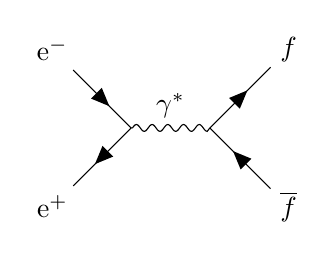
\begin{tikzpicture}
    \begin{feynman}
      \vertex (a) {$\mathrm{e^-}$};
      \vertex[below=2cm of a] (b) {$\mathrm{e^+}$};
      \vertex[right=1cm of a] (c);
      \vertex[below=1cm of c] (d);
      \vertex[right=1cm of d] (e);
      \vertex[right=3cm of a] (f) {$f$};
      \vertex[right=3cm of b] (g) {$\overline{f}$};
      \diagram* {
        (a) -- [fermion] (d) -- [fermion] (b),
        (d) -- [photon, edge label=\(\gamma^*\)] (e),
        (g) -- [fermion] (e) -- [fermion] (f),
      };
    \end{feynman}
  \end{tikzpicture}
\caption{\ee annihilation to a fermion-antifermion pair.}
  \label{fig:ee_to_ff_diagram}
\end{figure}

The ratio $R$ is given by
\begin{equation*}
    R = \frac{\sigma(e^+e^- \rightarrow \mathrm{hadrons})}{\sigma(e^+e^- \rightarrow \mu^+\mu^-)} = N_c \sum_f Q_f^2\ ,
\end{equation*}
where $N_c$ represents the number of existing colours and $Q_f$ is the electric charge of the quark flavour $f$. Notably, this ratio depends on centre-of-mass energy (\sqs) and encompasses all possible quark flavours that can be produced by the virtual photon at that specific energy level. While at low energies (few \gev) only light quarks ($u,d,s$) are produced, at higher energies, heavier quarks like charm ($c$, \mbox{$M_c=1.2730\pm0.0046~\gevcc$}~\cite{pdg}) and beauty ($b, M_b=4.183\pm0.007~\gevcc$~\cite{pdg}) can be produced as well. The experimental measurements of $R$, shown in Fig.~\ref{fig:R_vs_s}, exhibit a remarkable agreement with the predictions of the three-colour model, thereby providing compelling evidence for the existence of colour and fractional electric charge of quarks.

The final step that propelled the development of Quantum Chromodynamics (QCD) as a comprehensive theory of the strong force was the insight into the mechanism that ensured all hadron wavefunctions to be colour singlets. This emerged from the discovery of asymptotic freedom, a phenomenon observed in deep-inelastic scattering experiments. Non-Abelian gauge theories, often referred to as Yang-Mills theories, were identified as having this unique characteristic. This realisation led to the formulation of QCD by elevating the global colour $SU(3)$ symmetry to a local one, allowing the 8 quanta of the $SU(3)$ gauge field, called \emph{gluons}, to mediate the strong force, successfully describing the confinement and behavior of quarks and gluons within hadrons.

\begin{figure}[p]
    \centering
    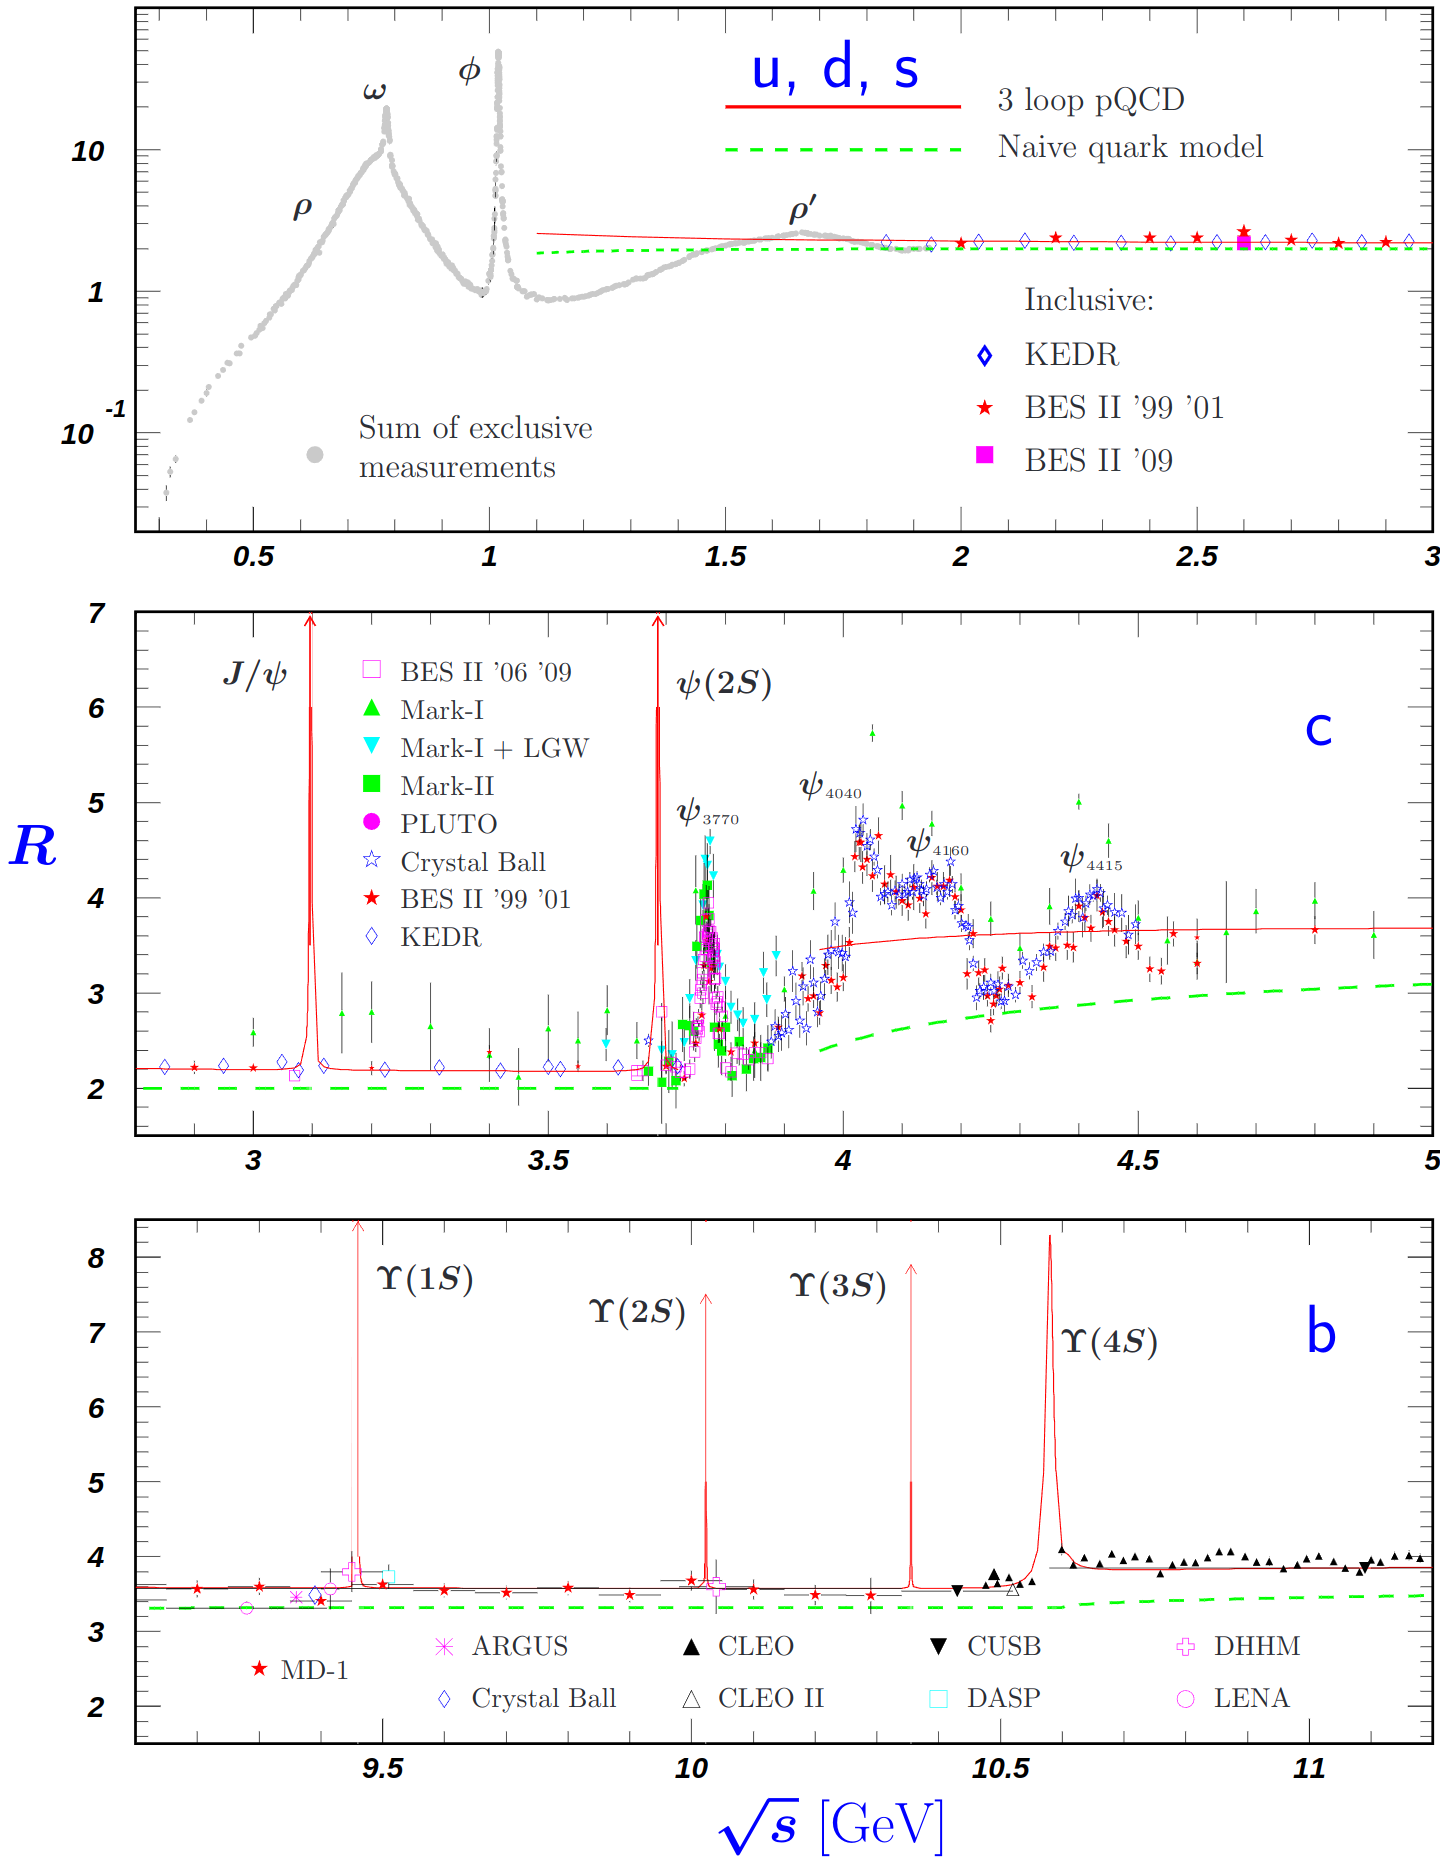
\includegraphics[width=\linewidth]{Figures/Chapter 1/rpp2022-R_udscb.png}
    \caption{$R$ as a function of $\sqrt{s}$ in the light-flavour, charm, and beauty threshold regions taken from Ref.~\cite{pdg}. The green curve is a naive quark-parton model prediction, while the red one is a 3-loops perturbative QCD prediction. Breit-Wigner parameterisations of $J/\psi$, $\psi$(2S), and $\Upsilon$(nS), n = 1,2,3,4 are also shown.}
    \label{fig:R_vs_s}
\end{figure}

The QCD Lagrangian density can be written as
\begin{equation}\label{eq:Lqcd}
    \mathcal{L}_{QCD}=-\frac{1}{4} F^a_{\mu\nu}F_a^{\mu\nu} + \sum_f \bar{q}_f^i (i\gamma^\mu(\mathcal{D}_\mu)_{ij}-m_f\delta_{ij})q_f^j\ ,
\end{equation}
where $F^a_{\mu\nu}$ is the field strength tensor defined in terms of the gluon field $A^a_\mu$ and the $SU(3)$ structure constant $f^{abc}$ as
\begin{equation} \label{eq:F}
    F^a_{\mu\nu} = \partial_\mu A^a_\nu - \partial_\nu A^a_\mu + g_s f^{abc}A^b_\mu A^c_\nu 
\end{equation}
and $(\mathcal{D}_\mu)_{ij}$ is the covariant derivative:
\begin{equation*}
    (\mathcal{D}_\mu)_{ij} = \partial_\mu \delta_{ij} - ig_s(t^a)_{ij}A_\mu^a\ ,
\end{equation*}
with $t^a$ being one of the generators of the $SU(3)$ representation.

The last term in Eq.~\ref{eq:F} is peculiar to non-Abelian theories, and gives rise to triplet and quartic gluon self-interactions illustrated in Fig.~\ref{fig:Feynman-gluons}. $g_s$ is a coupling parameter related to the strong coupling constant \als, which determines the strength of the interaction between the coloured particles.

\begin{figure}[htb]
    \centering
    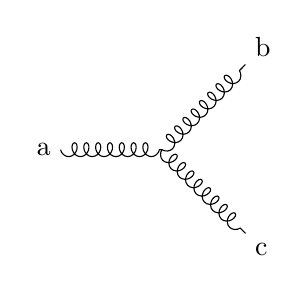
\begin{tikzpicture}
      \begin{feynman}
        \vertex (a) {a};
        \vertex [right=of a] (b);
        \vertex[above right= of b] (c) {b};
        \vertex[below right= of b] (d) {c};
        \diagram* {
          (a) -- [gluon] (b),
          (b) -- [gluon] (c),
          (b) -- [gluon] (d),
        };
      \end{feynman}
    \end{tikzpicture} \qquad
    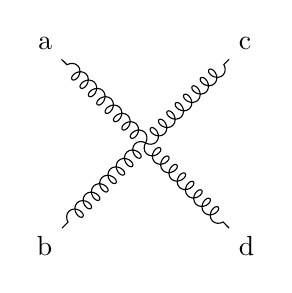
\begin{tikzpicture}
      \begin{feynman}
        \vertex (a);
        \vertex[above left=of a] (b) {a};
        \vertex[above right= of a] (c) {c};
        \vertex[below right= of a] (d) {d};
        \vertex[below left= of a] (e) {b};
        \diagram* {
          (a) -- [gluon] (b),
          (a) -- [gluon] (c),
          (a) -- [gluon] (d),
          (a) -- [gluon] (e),
        };
      \end{feynman}
    \end{tikzpicture}
    \caption{Feynman diagrams for gluon self-interactions.}
    \label{fig:Feynman-gluons}
\end{figure}

The second term of Eq.~\ref{eq:Lqcd} describes the interactions between quarks and gluons, sketched in Fig.~\ref{fig:Feynman_q_g}, and contains the mass term for the fermions. It is noteworthy to observe that the interaction between quarks and gluons is diagonal in flavour, meaning that the strong interaction conserves the flavour of quarks. In contrast, colour mixing is allowed within the framework of QCD.

\begin{figure}[htb]
    \centering
    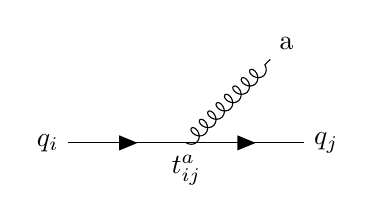
\begin{tikzpicture}
      \begin{feynman}
        \vertex (a);
        \vertex [below=0.1em of a] {$t^a_{ij}$};
        \vertex[left=of a] (b) {$q_i$};
        \vertex[right= of a] (c) {$q_j$};
        \vertex[above right= of a] (d) {a};
        \diagram* {
          (b) -- [fermion] (a),
          (a) -- [fermion] (c),
          (a) -- [gluon] (d),
        };
      \end{feynman}
    \end{tikzpicture}
    \caption{Feynman diagram for quark-gluon interaction.}
    \label{fig:Feynman_q_g}
\end{figure}

\subsection{Running coupling constant}
If one considers a dimensionless physical observable, denoted in the following as $R$, which solely depends on a single energy scale, $Q$, one might naturally expect $R$ to maintain a constant value, independent of the specific energy scale chosen. However, this does not hold true when loop diagrams are studied: the necessity of renormalisation introduces a new energy scale denoted as $\mu$. This scale, known as the renormalisation scale, is the point at which the subtraction of the ultraviolet divergences is carried out. Critically, $\mu$ is an arbitrary parameter and, as such, is non-physical. Consequently, $R$ becomes dependent on the ratio $Q^2/\mu^2$ and the renormalised coupling $\alpha_s = g_s^2/4\pi$: $R \equiv R\left(\frac{Q^2}{\mu^2},\als\right)$. The $\mu$ independence of $R$ (which is an essential requirement given $\mu$'s arbitrariness) can be expressed as
\begin{equation}\label{eq:RGE}
    \mu^2 \frac{\de R\left(\frac{Q^2}{\mu^2},\alpha_s\right)}{\de \mu^2} = \mu^2 \left[\frac{\partial}{\partial\mu^2}+\frac{\partial \alpha_s}{\partial\mu^2}\frac{\partial}{\partial\alpha_s}\right]R\left(\frac{Q^2}{\mu^2},\alpha_s\right) = 0\ , 
\end{equation}
a fundamental equation known as the renormalisation group equation. This equation is exactly true in the case of a prediction that considers all perturbative orders. If one limits the expansion at a fixed order $\als^\mathrm{N}$, then a dependence of $R$ from $\mu$ is observed at the $\als^\mathrm{N+1}$ order. By introducing
\begin{equation*}
    t\equiv \mathrm{log}(Q^2/\mu^2), \qquad \beta(\als)\equiv \mu^2 \frac{\de\als}{\mathrm{\de\mu^2}}\quad ,
\end{equation*}
Eq.~\ref{eq:RGE} can be written as
\begin{equation*}
    \left(-\frac{\partial}{\partial t} + \beta(\als)\frac{\partial}{\partial \als}\right) R(e^t,\als) = 0\quad .
\end{equation*}
This first-order partial differential equation can be solved by defining a new function: the running coupling $\als(Q^2)$, which evolves as a function of $Q$.
\begin{equation}\label{eq:t_integral}
    t = \mathrm{log}(Q^2/\mu^2) \equiv \int_{\als}^{\als(Q^2)} \frac{\de x}{\beta(x)} , \quad \mathrm{with}~\als=\als(\mu^2)\quad .
\end{equation}
By differentiating Eq.~\ref{eq:t_integral} with respect to $t$ and \als, one gets:
\begin{equation}\label{eq:beta_def}
    \beta(\als(Q^2)) = \frac{\partial\als(Q^2)}{\partial t}, \quad \frac{\de\als(Q^2)}{\de\als} = \frac{\beta(\als (Q^2))}{\beta(\als)}\quad .
\end{equation}
It results from this last set of equations that $R(1,\als(Q^2))$ satisfies Eq.~\ref{eq:RGE}; hence, the running coupling constant has absorbed the $\mu$ scale dependence of $R$. As a consequence, the knowledge of $R(1,\als)$, which can be evaluated in fixed-order perturbation theory, allows knowing the dependence of $R$ from $Q^2$, the physical scale at which the coupling is gauged, by simply substituting $\als \rightarrow \als(Q^2)$. 

\subsubsection{The \ensuremath{\beta} function}
The running of the coupling constant is determined by the $\beta(\als)$ function, which is evaluated from loop corrections to the bare vertices of QCD. As of the time of the writing of this Thesis, the $\beta$ function has been evaluated up to 5 loops~\cite{Herzog:2017ohr}. In Fig.~\ref{fig:beta_loops}, the 1-loop Feynman diagrams contributing to the $\beta$ function evaluation are reported.

\begin{figure}[htb]
    \centering
    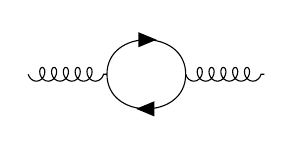
\begin{tikzpicture}
      \begin{feynman}
        \vertex (a);
        \vertex [right=1cm of a] (b);
        \vertex[right=1cm of b] (c);
        \vertex[right=1cm of c] (d);
        \diagram* {
            (a) -- [gluon] (b)
            -- [fermion, half left, looseness=1.5] (c)
            -- [fermion, half left, looseness=1.5] (b),
            (c) -- [gluon] (d),
        };
      \end{feynman}
    \end{tikzpicture}\quad
    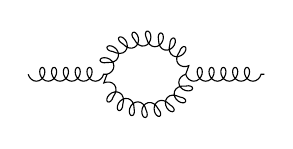
\begin{tikzpicture}
      \begin{feynman}
        \vertex (a);
        \vertex [right=1cm of a] (b);
        \vertex[right=1cm of b] (c);
        \vertex[right=1cm of c] (d);
        \diagram* {
            (a) -- [gluon] (b)
            -- [gluon, half left, looseness=1.5] (c)
            -- [gluon, half left, looseness=1.5] (b),
            (c) -- [gluon] (d),
        };
      \end{feynman}
    \end{tikzpicture}\quad
    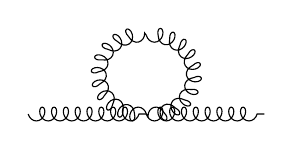
\begin{tikzpicture}
      \begin{feynman}
        \vertex (a);
        \vertex [right=of a] (b);
        \vertex[above=1cm of b] (c);
        \vertex[right=of b] (d);
        \diagram* {
            (a) -- [gluon] (b)
            -- [gluon, half left, in=90, looseness=2] (c)
            -- [gluon, half left, in=90, looseness=2] (b),
            (b) -- [gluon] (d),
        };
      \end{feynman}
    \end{tikzpicture}\quad

    \vspace{0.6cm}
    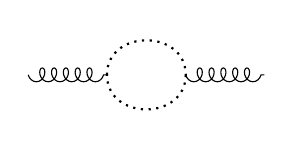
\begin{tikzpicture}
      \begin{feynman}
        \vertex (a);
        \vertex [right=1cm of a] (b);
        \vertex[right=1cm of b] (c);
        \vertex[right=1cm of c] (d);
        \diagram* {
            (a) -- [gluon] (b)
            -- [ghost, half left, looseness=1.5] (c)
            -- [ghost, half left, looseness=1.5] (b),
            (c) -- [gluon] (d),
        };
      \end{feynman}
    \end{tikzpicture}\quad
    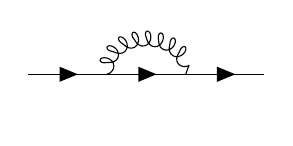
\begin{tikzpicture}
      \begin{feynman}
        \vertex (a);
        \vertex [right=1cm of a] (b);
        \vertex[right=1cm of b] (c);
        \vertex[right=1cm of c] (d);
        \vertex[below=0.31cm of c] (f) {$ $};
        \diagram* {
            (a) -- [fermion] (b) -- [fermion] (c) -- [fermion] (d),
            (b) -- [gluon, half left, looseness=1.5] (c)
            
        };
      \end{feynman}
    \end{tikzpicture}\quad
    
    \vspace{0.5cm}
    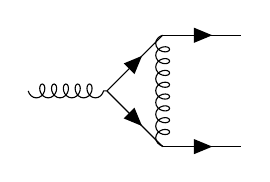
\begin{tikzpicture}
      \begin{feynman}
        \vertex (a);
        \vertex [right=1cm of a] (b);
        \vertex[above right=1cm of b] (c);
        \vertex[right=1cm of c] (d);
        \vertex[below right=1cm of b] (e);
        \vertex[right=1cm of e] (f);
        \diagram* {
            (a) -- [gluon] (b) -- [fermion] (c) -- [fermion] (d),
            (b) -- [fermion] (e) -- [fermion] (f),
            (c) -- [gluon] (e)
        };
      \end{feynman}
    \end{tikzpicture}\quad
    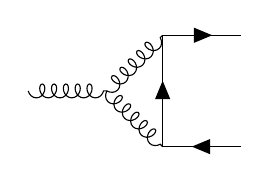
\begin{tikzpicture}
      \begin{feynman}
        \vertex (a);
        \vertex [right=1cm of a] (b);
        \vertex[above right=1cm of b] (c);
        \vertex[right=1cm of c] (d);
        \vertex[below right=1cm of b] (e);
        \vertex[right=1cm of e] (f);
        \diagram* {
            (a) -- [gluon] (b) -- [gluon] (c),
            (b) -- [gluon] (e),
            (f) -- [fermion] (e) -- [fermion] (c) -- [fermion] (d)
        };
      \end{feynman}
    \end{tikzpicture}\quad
    \caption{1-loop Feynman diagrams contributing to the $\beta$ function evaluation.}
    \label{fig:beta_loops}
\end{figure}

By limiting the calculations at the first order in the perturbative expansion, one gets:
\begin{equation}\label{eq:beta0}
    \beta(\als) = -\als^2 \frac{11 \mathrm{N_c} - 2 \mathrm{N_f}}{12\pi} + \mathcal{O}(\als^3) \equiv -\als^2 \beta_0 + \mathcal{O}(\als^3)\quad ,
\end{equation}
where $\mathrm{N_c}$ is the number of colours (3), while $\mathrm{N_f}$ is the number of quark flavours that can be considered massless at the physical scale $Q^2$ at which the coupling is being measured.
From Eqs.~\ref{eq:beta_def} and~\ref{eq:beta0}, one can extract the $Q^2$ dependency of the running coupling constant:
\begin{equation}\label{eq:alpha_s_running}
    \alpha_s(Q^2) = \frac{\alpha_s(\mu^2)}{1+\alpha_s(\mu^2)\beta_0 \mathrm{log}(Q^2/\mu^2)}\ ,
\end{equation}

Notably, since $\beta_0$ is positive in a six-quark-flavour framework, the strong coupling constant exhibits a monotonic decreasing trend as a function of $Q^2$. This behaviour differs from the one of the electromagnetic coupling constant, which increases with the energy scale due to the screening effect of vacuum polarisation. For QCD, the running of the coupling constant is a direct consequence of the non-Abelian nature of the theory, allowing for gluon self-interactions, which give rise to an anti-screening effect. The idea is that the emission of virtual gluons by static colour sources causes their colour charges to 'leak out' into the surrounding vacuum. Since the interaction between distributions of charges is weaker than the one between point-like charges when the distributions overlap, the effective coupling constant decreases at short distances. This behaviour is known as asymptotic freedom, a key feature of QCD that allows for the perturbative expansion of the theory at high energy scales, where the strong coupling constant is small. At the same time, the running of the coupling constant implies that the theory is non-perturbative at low energy scales, and phenomenological models are required to describe the strong interaction in this regime. 

Instead of using the renormalisation scale $\mu$ as a free parameter, one can use the running coupling constant to define a physical scale, $\Lambda_\mathrm{QCD}$, which is the energy scale at which the coupling constant would diverge, if extrapolated outside the perturbative regime. Using Eq.~\ref{eq:alpha_s_running}, one can write
\begin{equation*}
    \alpha_s(\Lambda_\mathrm{QCD}) = \frac{1}{\beta_0 \mathrm{log}(Q^2/\Lambda_\mathrm{QCD}^2)}\quad .
\end{equation*}
The value of $\Lambda_\mathrm{QCD}$ is determined by the specific definition being used. However, to obtain the value of the coupling constant measured at $Q^2 = M_\mathrm{Z}^2$, an approximate value of $\Lambda_\mathrm{QCD}$ of around 200~\mev can be used.

Measurements of the running of the coupling constant at different values of $Q$ are illustrated in Fig.~\ref{fig:alpha_s_running} and compared to the theoretical prediction at 5 loops. The agreement between the experimental data and the theoretical prediction is remarkable, confirming the validity of the QCD framework at high energy scales.


\begin{figure}[htb]
    \centering
    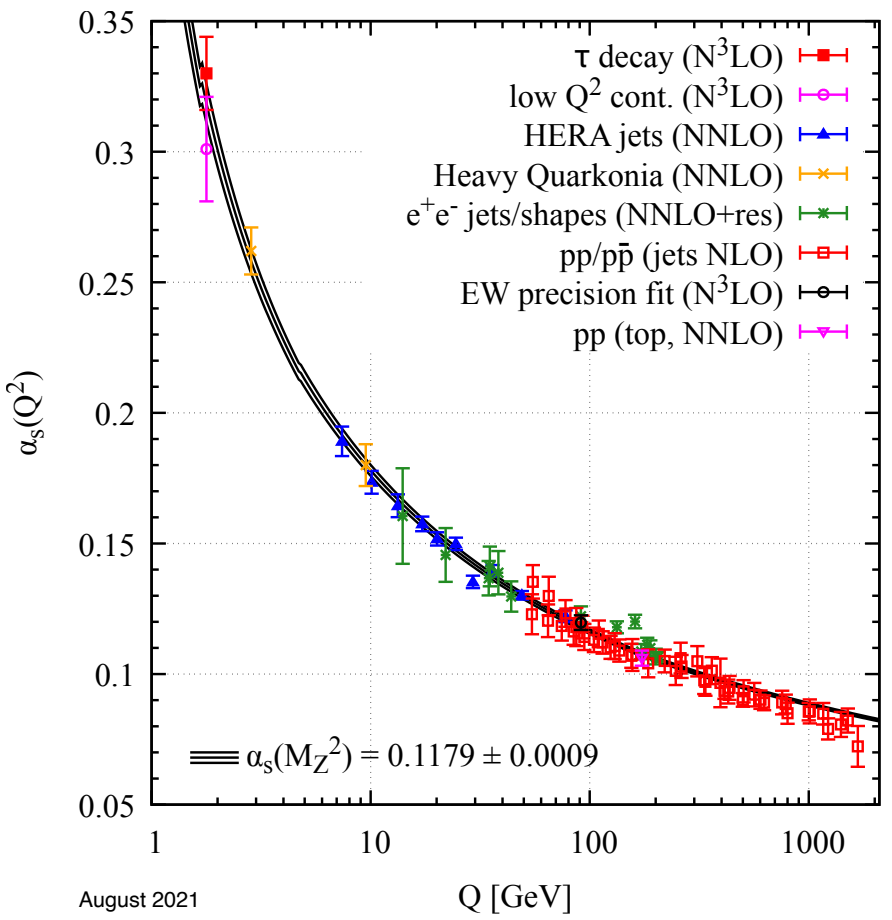
\includegraphics[width=0.7\linewidth]{Figures/Chapter 1/Alpha_s_running.png}
    \caption{Summary of measurements of \als as a function of the energy scale $Q$, compared to the running of the coupling computed at five loops, taking as an input the current PDG average, $\als(M_\mathrm{Z}^2) = 0.1180 \pm 0.0009$ \gevcc. Figure taken from Ref.~\cite{pdg}.}
    \label{fig:alpha_s_running}
\end{figure}

\section{Confinement}
The concept of confinement is one of the most intriguing aspects of QCD. It is the phenomenon by which quarks and gluons are never observed as free particles, but are always confined within colour-neutral hadrons. The confinement of quarks and gluons is a direct consequence of the non-Abelian nature of the theory, which, as described in the previous Section, is characterised by an increase in the strong coupling constant at low energy scales. The confinement of quarks and gluons is a non-perturbative effect, and despite extensive research, a comprehensive theoretical description of confinement in QCD remains elusive. Phenomenological models like the MIT bag model have been proposed, but a full comprehension of confinement is still lacking. Lattice QCD simulations are the most successful approach to study the non-perturbative regime of the theory, and they have provided a wealth of information on the properties of hadrons and the strong interaction at low energy scales.

\subsection{MIT bag model}
The MIT bag model~\cite{Johnson:1975zp} is a phenomenological model of confinement, which describes hadrons as bound states of quarks and gluons confined within a finite volume, called \emph{bag}. The model was developed in the 1970s by A. Chodos, R. L. Jaffe, K. Johnson, C. B. Thorn, and V. F. Weisskopf, and it has been widely used to study the properties of hadrons and strong interactions. In the MIT bag model, N non-interacting massless fermions are confined within a spherical cavity of radius $R$, which is the bag radius. The confinement arises from a balance between the pressure due to the kinetic energy of the fermions inside the bag and an ad hoc external pressure, which is introduced to confine the fermions within the bag. The fermions are described by the Dirac equation for massless fermions:

\begin{equation*}
    i\gamma^\mu\partial_\mu\psi = 0\quad ,
\end{equation*}
where $\psi$ is the fermion field, and $\gamma^\mu$ are the Dirac matrices. The solution to the Dirac equation is given in terms of the spherical Bessel functions of zeroth and first order, $j_0(p_0r)$ and $j_1(p_0r)$:

\begin{equation*}
    \psi = \mathcal{N} e^{-ip_0t} \begin{pmatrix} j_0(p_0r)\chi^+ \\ \vec{\sigma}\cdot\hat{r}j_1(p_0r)\chi^-\end{pmatrix}\quad ,
\end{equation*}
where $p_0$ is the energy of the fermion, $\chi^+$ and $\chi^-$ are the two components of the fermion four-dimensional spinor $\psi$, and $\vec{\sigma}$ are the Pauli matrices. The colour flux at a point $r$ inside the bag is given by

\begin{equation*}
    j_{ab}^\mu(r) = \bar{\psi_a}(r)\gamma^\mu\psi_b(r)\quad ,
\end{equation*}
where $a$ and $b$ are the colour indices of the fermions. If the quantum numbers are not to be lost through the surface of the bag, which is the definition of confinement, then, on the surface:

\begin{equation*}
  n_\mu j_{ab}^\mu(r) = \bar{\psi_a}(r)\gamma\cdot n \psi_b(r) = 0\quad ,
\end{equation*}
 where $n_\mu$ is a unit space-like vector perpendicular to the surface. Using the gamma properties, $(i\gamma\cdot n)^2 = 1$, so that by assuming that $i\gamma\cdot n = + 1$, the boundary condition on the surface of the bag is given by

\begin{equation*}
    \bar{\psi}(R)\psi(R) = 0\quad ,
\end{equation*}
leading to the solution of the Dirac equation in the bag:

\begin{equation*}
    \left[j_0\left(p_0R\right)\right]^2 - \left[j_1\left(p_0R\right)\right]^2 = 0\quad ,
\end{equation*}
with solution $p_0R = 2.04$. The total energy inside the bag is given by

\begin{equation*}
    E = \frac{2.04 \mathrm{N}}{R}(\hbar c) + \frac{4\pi}{3}R^3B\quad ,
\end{equation*}
where the first term is the kinetic energy of the fermions, and the second term is the energy due to the presence of an external pressure $B$ which keeps the fermions confined in the bag. The bag pressure is a phenomenological parameter of the model, and it is introduced to confine the fermions within the bag. It can be extracted by minimising the energy of the system with respect to the bag radius $R$, which yields $B=234$~\mev/fm$^3$ for a baryon with $R=0.8$ fm.

\subsection{Lattice QCD}
Lattice QCD is a numerical technique used to study the non-perturbative regime of QCD. The method is based on the discretisation of space-time on a four-dimensional lattice, and the evaluation of the path integral of the theory using Monte Carlo methods, i.e. by sampling possible configurations of the quark and gluon fields according to the probability distribution given by the QCD Lagrangian. The lattice spacing is a parameter of the method, and allows one to avoid the ultraviolet divergences of the theory, which are typical in perturbative QCD, by introducing a cutoff on the momenta of the quark and gluon fields. 
\begin{figure}[htb]
  \centering
  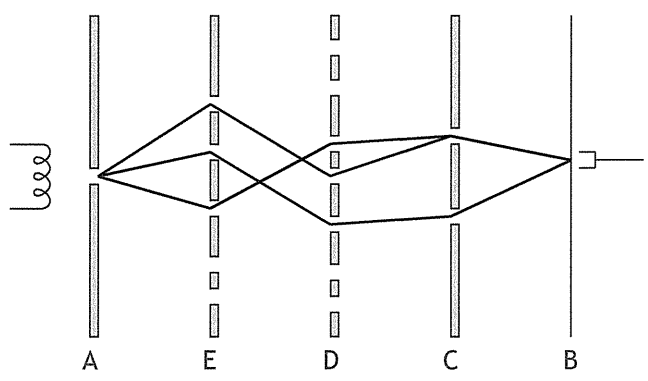
\includegraphics[width=0.7\linewidth]{Figures/Chapter 1/PathIntegrals.png}
  \caption{Feynman introduction to path integrals. Here, a particle emitted from a source at $x_a$ is detected at $x_b$. A finite number of screens, each with a finite number of holes, is placed between the source and the detector. The probability amplitude for the particle to hit the detector is given by the sum of the probabilities of moving from the source to the detector through all possible paths. By adding an infinite amount of screens with an infinite number of holes, and by also considering the time at which the particle passes through each screen, the sum becomes an integral over all possible paths, called a \emph{path integral}.}
  \label{fig:PathIntegrals}
\end{figure}

The Lattice QCD simulations are based on the path integral formalism of quantum field theory~\cite{RevModPhys.20.367}, developed by R. Feynman in the 1940s. The path integral provides a natural extension to quantum mechanics of the least action principle of classical mechanics, and it allows one to calculate the probability amplitude of a particle to move from one point to another in space-time, considering the evolution of the system over all possible paths. The transition amplitude from the state $(x_a,t_a)$ to the state $(x_b,t_b)$ is given by
\begin{equation}\label{eq:ampl_prob}
  A \left[(x_a,t_a) \rightarrow (x_b,t_b) \right] = \braket{x_b,t_b | e^{-iH(t_b-t_a)} | x_a,t_a} = \sum_\mathrm{paths} e^{iS[x(t)]}\quad , 
\end{equation}
where $H$ is the Hamiltonian of the system, $S[x(t)]$ is the action of the system for a given path $x(t)$, and the sum runs over all possible paths from $(x_a,t_a)$ to $(x_b,t_b)$. By taking the continuum limit on space-time, one obtains an integration over all the possible space-time paths of the system:
\begin{equation}\label{eq:path_integral}
  \sum_\mathrm{paths} e^{iS[x(t)]} \rightarrow \int_{x_a}^{x_b} \left[\mathcal{D}x(t)\right] e^{iS[x(t)]}\quad ,
\end{equation}
where the right-hand side term is a functional integral over all possible paths. It is interesting to note that by combining Eqs.~\ref{eq:ampl_prob} and \ref{eq:path_integral}, a quantity resembling the partition function of a statistical system is obtained:
\begin{equation*}
  \mathcal{Z} = \sum_{x_a} \braket{x_a,t_a | e^{\beta H} | x_a,t_a}\quad .
\end{equation*}
It is possible to express the partition function in terms of a path integral by applying a Wick rotation to the time variable, $t \rightarrow -i\tau$, with $\tau_a=0\leq\tau\leq\tau_b=\beta$ and considering the Euclidean action in place of the Minkowskian one, $S_\mathrm{E}=iS$. Furthermore, since the state at $\tau_a$ is the same as the one at $\tau_b$ in the partition function definition, a periodic boundary condition is imposed: $x(\tau_a) = x(\tau_b)$. With these considerations, the partition function can be expressed as
\begin{equation*}
  \mathcal{Z} = \int \left[\mathcal{D}x(\tau)\right] e^{-S_\mathrm{E}[x(\tau)]}\quad .
\end{equation*}
This formalism, which was here developed for a single particle, can be extended to a quantum field theory, and in particular to QCD.

Lattice QCD simulations are computationally intensive, and they require large supercomputers to perform the calculations. To limit the computational costs, calculations are often performed at larger up and down quark masses than in nature, drastically reducing the number of virtual quark-antiquark loops that have to be taken into account. Because of the employed Monte Carlo approach, only a finite number of configurations can be considered, leading to statistical uncertainties in the lattice QCD results. In order to obtain physical results, several limits have to be taken: i) the continuum limit, i.e. the extrapolation of the lattice spacing to zero, ii) the infinite-volume limit, i.e. the extrapolation of the lattice size to infinity, and iii) the physical quark-mass limit, i.e. the extrapolation to physical quark masses. Many present-day lattice calculations are already performed directly at, or very close to, the physical values of the quark masses~\cite{BMW:2008jgk,BMW:2014pzb,Bazavov:2017dus}, so that the latter extrapolation becomes less of an issue. 

The results of the lattice QCD simulations are in good agreement with the experimental data as shown in Fig.~\ref{fig:LQCD_hadron_mass} for the spectrum of hadron masses obtained from lattice QCD simulations, taken from Ref.~\cite{BMW:2008jgk}.
\begin{figure}[t!]
  \centering
  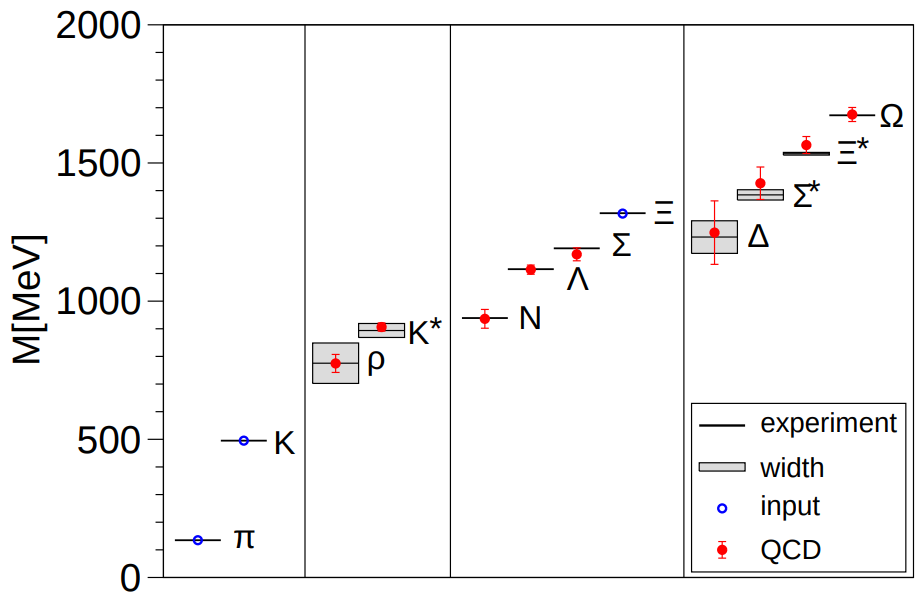
\includegraphics[width=0.7\linewidth]{Figures/Chapter 1/LQCD_hadron_mass.png}
  \caption{The light hadron mass spectrum of QCD. Horizontal lines and bands are the experimental values with their decay widths. Lattice QCD results~\cite{BMW:2008jgk} are shown by solid circles. Vertical error bars represent the combined statistical and systematic error estimates. $\pi$, K, and $\Xi$ have no error bars, because they are used to set the light quark mass, the strange quark mass, and the overall scale, respectively.}
  \label{fig:LQCD_hadron_mass}
\end{figure}

\section{Quark--Gluon Plasma}
The concept of deconfinement refers to the transition from a confined state to a state where quarks and gluons are no longer confined within colour-neutral hadrons, but can move in a larger volume. As modelled by the MIT bag model, non-perturbative QCD effects can be described in terms of an external pressure, which confines quarks and gluons within a finite volume. If the external pressure is overcome by the pressure due to the kinetic energy of the quarks and gluons, then the hadrons constituents are no longer confined, and a transition to a state called Quark-Gluon Plasma (QGP) occurs. Lattice QCD calculations are used to understand the properties of the QGP, and they predict that a strongly interacting system with zero net baryon density evolves smoothly from a confined (hadronic) towards a deconfined (partonic) state when its temperature is increased up to $\sim155$~\mev~\cite{HotQCD:2014kol, Borsanyi:2013bia} ($1.8\times 10^{12}$ K, around $10^6$ times the temperature of the core of the Sun), reaching energy densities of $\sim 0.5$~\gev/fm$^3$~\cite{Bazavov:2017dus}.

\begin{figure}
  \centering
  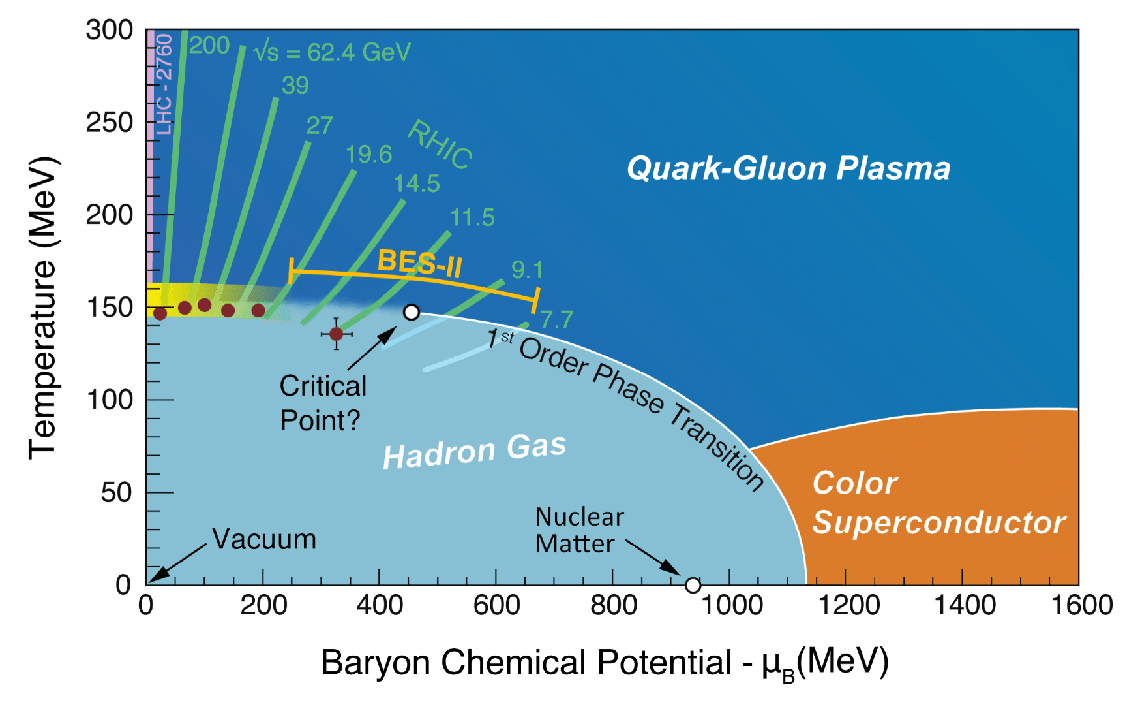
\includegraphics[width=0.7\linewidth]{Figures/Chapter 1/QCD-diagram.jpg}
  \caption{QCD phase diagram in the temperature-baryon chemical potential plane. Figure taken from Ref.~\cite{QCD_diagram}.}
  \label{fig:PhaseDiagram}
\end{figure}

It is believed that the Universe underwent a phase of deconfinement in the early stages of its evolution, few microseconds after the Big Bang~\cite{rafelski2014traveling}. Direct observation of the primordial QGP (i.e. that created just after the Big Bang) would provide a wealth of information on the early Universe; however, the Universe experienced a phase in which electrons were not bound into atoms (electromagnetic plasma), making it opaque to electromagnetic radiation, and denying us the possibility of directly observing the primordial QGP. Once the Universe cooled enough (3000~K) to allow electrons to bind to nuclei, the electromagnetic radiation decoupled with a black body spectrum of around 3000 K. Since then, as the Universe expanded, this electromagnetic radiation has redshifted to a temperature of around 2.7~K, and is denoted as the Cosmic Microwave Background (CBM). The CMB is the oldest light in the Universe and provides a snapshot of the Universe when it was 300'000 years old, long after the QGP phase. Although recent studies evidenced the presence of QGP in massive neutron star cores~\cite{Annala:2019puf}, a more controlled environment for studying the QGP is achieved by recreating it in laboratories, through the collision of heavy ions at ultra-relativistic energies. In the past decades, several experiments~\cite{ALICE:2022wpn, NA38:2000wlp, NA50:1997hlx, Nouicer:2009fy} have been carried out to study the properties of this state of matter, and the results have provided valuable insights into the properties of the strongly-interacting matter.

\subsection{High-energy heavy-ion collisions}
\begin{figure}[t]
  \centering
  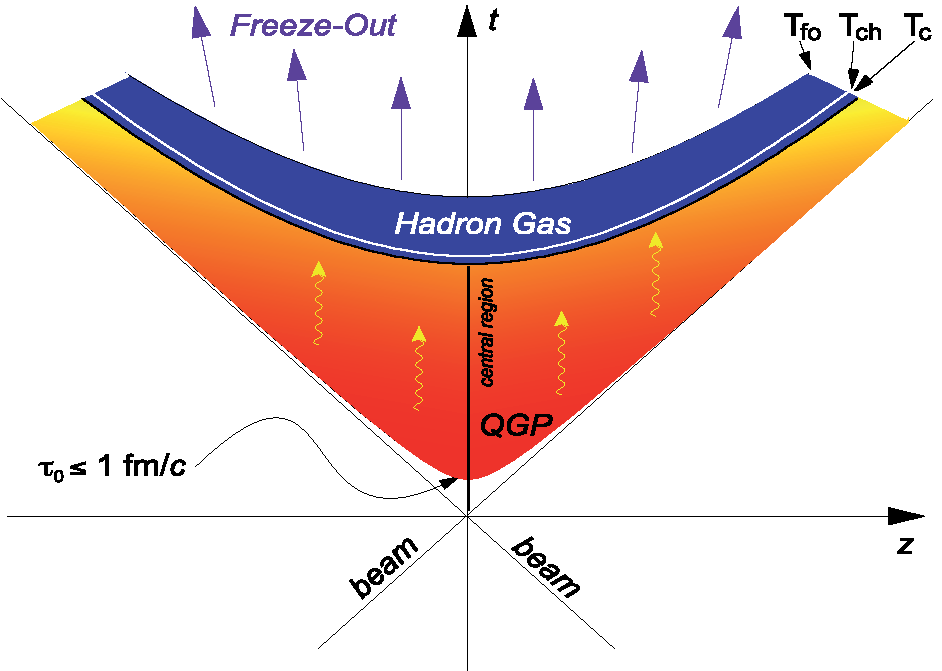
\includegraphics[width=0.7\linewidth]{Figures/Chapter 1/Bild_18.pdf}
  \caption{Space-time evolution of a heavy-ion collision. Figure taken from Ref.~\cite{Stock:2008ru}.}
  \label{fig:HeavyIonCollisions}
\end{figure}
Heavy-ion collisions are the most suitable environment to study the properties of the QGP in the laboratory. In these collisions, two heavy ions, such as lead or gold nuclei, are accelerated to ultra-relativistic energies and made to collide. Given the large amount of energy deposited in the collision, the system reaches high energy densities (of around 16 \gev/fm$^3$ after 1 fm/$c$ for central collisions at the LHC~\cite{Loizides:2011ys}), which allow for the production of the QGP for temperatures $T>T_\mathrm{pc}$, where $T_\mathrm{pc}$ is the pseudo-critical temperature for the transition to a deconfined state, as shown in Fig.~\ref{fig:PhaseDiagram}. As nuclei are objects made of many nucleons (i.e.\ protons and neutrons), the interaction volume (called \emph{fireball}) is larger and longer-lived than in proton-proton collisions, allowing the usage of thermodynamics and hydrodynamics to describe the system created in the collision. 

It is possible to distinguish between two different collision regimes, which probe different phase spaces in the QCD diagram reported in Fig.~\ref{fig:PhaseDiagram}. The ordinary nuclear matter is located at approximately $T\sim0$ and $\mu_mathrm{B}=1$~\gev, where $\mu_mathrm{B}$ is the baryo-chemical potential, expressing the energy needed to increase the baryon number of the system by one unit, as described in Sec.~\ref{subsec:SHM}. When the centre-of-mass energy per nucleon pair (\snn) is below a few \gev, the nucleons of the colliding nuclei are stopped in the collision as they lose energy and momentum. Due to conserved currents, the quantum numbers of the initial state are preserved, so that, for example, the net baryon production (i.e. the difference between the number of produced baryons and antibaryons) is positive. This regime is called \emph{stopping regime}. In this regime, the baryo-chemical potential is increased by about 5--10 times with respect to that of nuclear matter. When the \snn increases, the initial state baryon number is carried away by the receding nucleons, and the net baryon number in the fireball at midrapidity ($y\sim0$) is zero. The rapidity is defined as 
\begin{equation*}
    y = \frac{1}{2}\mathrm{log}\left(\frac{E+p_z}{E-p_z}\right)\quad ,
\end{equation*}
where $E$ is the energy and $p_z$ is the longitudinal momentum of the particle. In this regime, denoted as \emph{Bjorken regime}, or \emph{transparency regime}, high temperatures of a few hundred \mev are reached, and $\mu_\mathrm{B}$ is close to 0.   

The collision of two nuclei is a rather complex process, with a space-time evolution that can be divided into several stages, as depicted in Fig.~\ref{fig:HeavyIonCollisions}. They can be studied by measuring different final-state observables that are sensitive to such stages. One of the first descriptions of the fireball evolution was given by J. Bjorken~\cite{Bjorken:1982qr}, who proposed a simple model to describe the expansion of the system in the longitudinal direction. In this model, it is assumed that there exists a central-plateau structure in the inclusive particle productions as a function of rapidity. In other terms, the Bjorken model assumes that the system is boost-invariant, i.e. independent of the longitudinal velocity. According to this model, the evolution of the system is described by the following stages: i) collision of the two nuclei, ii) pre-equilibrium, iii) QGP formation and expansion, iv) hadronisation and hadron gas expansion, and v) freeze-out.

\subsubsection{Collision}
The two nuclei are accelerated to ultra-relativistic energies and are thus Lorentz-contracted in the direction of motion. The collision takes place in a very short time $\tau_\mathrm{coll} = 2R/\gamma$, where R is the nucleus radius and $\gamma$ the Lorentz factor. At LHC energies, the crossing time of the nuclei is of $\sim 0.005$~fm/$c$, which is much smaller than the time scale of the strong interaction $\tau_\mathrm{strong} \sim 1/\Lambda_\mathrm{QCD} \sim 1$~fm/$c$. Particles produced in the collision through parton interactions mediated by the strong force are thus created once the colliding nuclei have already passed through each other and moved away from the interaction region. During the collision, a large amount of energy is deposited in the interaction region, leading to the formation of a fireball with high energy densities.

\subsubsection{Pre-equilibrium}
After $\tau_\mathrm{coll}$, secondary particles are produced from the energy deposited in the collision. In the Bjorken regime, it is possible to evaluate the energy density of the system as a function of time by measuring the transverse energy of the particles produced at midrapidity, where the net baryon density is zero. The energy density is given by
\begin{equation*}
    \varepsilon_\mathrm{Bjorken} = \frac{\braket{m_\mathrm{T}}}{\tau A} \left. \frac{\de N}{\de y}\right\rvert_{y=0} = \frac{1}{\tau A}\left. \left\langle\frac{\de E_\mathrm{T}}{\de y}\right\rangle\right\rvert_{y=0} \quad ,
\end{equation*}
where $A$ is the transverse area collision region, $\braket{m_\mathrm{T}}$ is the mean transverse mass, defined as $m_\mathrm{T} = \sqrt{m^2 + \pt^2}$, $N$ is the number of secondary particles, and $\braket{\de E_\mathrm{T}/\de y}$ is the mean transverse energy density. It is interesting to evaluate the energy densities reached at the time of particle formation, which can be estimated using Heisemberg's uncertainty principle: $\tau = \hbar/m_\mathrm{T}$. The mean transverse mass of the particles produced in the collision at the proper time of formation $\tau_\mathrm{f}$ can be evaluated using the approximate formula:
\begin{equation*}
    \braket{\mt} = \frac{\frac{\de \et(\tau_\mathrm{f})}{\de y}}{\frac{\de N(\tau_\mathrm{f})}{\de y}}\sim \left. \frac{\frac{\de \et}{\de \eta}}{\frac{\de N}{\de \eta}}\right\rvert_\mathrm{final~state}\quad ,
\end{equation*}
leading to a formation time of $\sim 0.35$~fm/$c$ in Au--Au collisions at $\snn=200$~\gevc at RHIC~\cite{PHENIX:2004vcz}, to which corresponds an energy density of $\sim 15$~\gev/fm$^3$. Measurements at LHC energies yield a higher energy density than RHIC by about a factor of 2.3~\cite{ALICE:2016igk}.

\subsubsection{Quark-gluon plasma formation}
The system of produced particles reaches thermal equilibrium through multiple scatterings at a proper time $\tau_\mathrm{eq}$, and the QGP is formed. Its evolution can be described using relativistic hydrodynamics. Studies at RHIC allow to constrain $\tau_\mathrm{eq}$ in the range of $0.6<\tau_\mathrm{eq}<1$~fm/$c$, corresponding to energy densities of $5.4 < \varepsilon_\mathrm{Bjorken}(\tau_\mathrm{eq})< 9$~\gev/fm$^3$, well above the threshold for QGP formation.
\subsubsection{Hadronisation}
The deconfined system expands and cools down, until the temperature decreases below the pseudo-critical value for the transition crossover ($T_\mathrm{pc}\sim 155-165$~\mev). The QGP undergoes a transition and hadronises, producing an expanding gas of colour-neutral particles. At LHC energies, this is expected to happen $\sim 10$~fm/$c$~\cite{ALICE:2011dyt} after the QGP formation. This transition is associated with a sharp decrease in the entropy density of the system.

\subsubsection{Freeze-out}
During the hadron gas expansion, the particle density decreases to a point where the inelastic interactions cease. The moment in which this happens is called \emph{chemical freeze-out}, and takes place at around $T_\mathrm{chem.}\sim160$~\mev~\cite{Andronic:2017pug}. This temperature value is very close to $T_\mathrm{pc}$, suggesting that the chemical freeze-out takes place very close to, or simultaneously with, the hadronisation. The chemical composition of the hadron gas cannot vary anymore, although elastic interactions, which change the momentum spectrum of the produced particles still occur. Once the temperature decreases below $T_\mathrm{therm.}\sim 130$~\mev, the elastic interactions cease as well, and this is referred to as \emph{thermal freeze-out}. The particles then keep expanding without interactions (\emph{free-streaming}), and are detected by the experimental apparatus.

\subsection{Hadron species abundances}\label{subsec:SHM}
Measurements of the multiplicity of identified hadron species, i.e., the chemical composition of the system, allow for the investigation of various properties of the system at the time of chemical freeze-out. The relative abundances of different hadron species produced in hadronic collisions are found to be well described by the \emph{Statistical Hadronisation Model} (SHM)~\cite{Braun-Munzinger:2003pwq}. The SHM is based on the assumption that the fireball created in an ultra-relativistic heavy-ion collision is in thermal and chemical equilibrium at the time of chemical freeze-out, which is assumed to be characterised by the same temperature for all the hadronic species.

A system is in thermal equilibrium when the distribution of particle velocities follows a Maxwell-Boltzmann distribution, which depends solely on the temperature of the system. Chemical equilibrium is achieved when the relative multiplicities of the different hadron species are described by their mass, spin degeneracy, and the temperature of the system. The hypothesis of thermal and chemical equilibrium is postulated, and allows the use of statistical mechanics to describe the system by defining a partition function that characterises the statistical properties of a system in equilibrium. The validity of this assumption is then verified a posteriori by comparing the model predictions with the experimental data. The equilibrium at the chemical freeze-out is purely statistical, i.e. the particle abundances are determined through the principle of maximum entropy, which suggests that hadronisation fills the phase space in the most probable configuration. Furthermore, the SHM does not take into account the dynamics of the system, but only its state at the time of the chemical freeze-out, without any assumption on the presence of a partonic phase. 

The system is described in the SHM picture in terms of a non-interacting gas of hadrons and resonances, which corresponds, in a Yukawa approach, to a hadron gas interacting through the exchange of resonances. This framework was found to be consistent with the equation of state of strongly-interacting matter from lattice QCD for temperatures below the pseudo-critical temperature of the QCD phase transition~\cite{HotQCD:2014kol}. 

The ensemble used to describe the system is the grand canonical ensemble, which describes a system exchanging energy and particles with the environment. In a grand canonical ensemble, the energy and the quantum numbers are conserved on average, but not exactly and locally as in a micro canonical ensemble. The fireball produced in an ultra-relativistic heavy-ion collision can be described in terms of small clusters that exchange energy and particles with the rest of the system. Smaller collision systems such as pp and \ee collisions, where fewer particles are produced, are described by the canonical ensemble, where the quantum numbers are conserved exactly and locally, while the energy is conserved on average.

The density of the hadron species i in the system can be calculated from the partition function $Z_\mathrm{i}^\mathrm{GC}$ and is given by
\begin{equation*}
    n_i = \frac{1}{V} \frac{\partial(TZ_\mathrm{i}^\mathrm{GC})}{\partial\mu_\mathrm{i}} = \frac{g_\mathrm{i}T^2}{2\pi^2}\sum_\mathrm{k=1}^\infty \frac{(\pm1)^\mathrm{k+1}}{k}\lambda_\mathrm{i}^\mathrm{k}m^2_\mathrm{i} K_2\left(\frac{\mathrm{k}m_\mathrm{i}}{T}\right) \quad ,
\end{equation*}
where $V$ is the volume of the system, $g_\mathrm{i}$, $\lambda_\mathrm{i} = e^{\mu_\mathrm{i}/T}$ and $m_\mathrm{i}$ are the degeneracy factor, the fugacity, and the mass of the hadron species i, respectively. The $+$ sign holds for bosons, while the $-$ sign is for fermions. $K_2$ is the second-order modified Bessel function of the second kind. The chemical potential $\mu_\mathrm{i}$ of the hadron species i is related to the conservation (on average, on a large volume) of the quantum numbers of the system. It is given by $\mu = \sum_\mathrm{j} \mu_{Q_\mathrm{j}}  Q_\mathrm{j}$, where $Q_\mathrm{j}$ are the conserved quantum numbers (third component of isospin, strangeness, and baryon number), and $\mu_{Q_\mathrm{j}}$ are the chemical potentials, which guarantee the conservation of the conserved charges. $\mu_\mathrm{i}$ is thus the energy needed to add a particle with quantum numbers $Q_\mathrm{j}$ to the system. The obtained multiplicities of the hadron species are then corrected with a feed-down contribution from decays of short-lived particles, which cannot be detected directly.

Of the five free parameters of the SHM ($T$, $\mu_{B}$, $\mu_{s}$, $\mu_{I_\mathrm{3}}$, and $V$), two can be fixed through conservation of the initial state quantum numbers. Particle abundances are typically fitted in terms of the temperature $T$, the baryon chemical potential $\mu_{B}$ and the volume of the system $V$. 

\begin{figure}[htb]
  \centering
  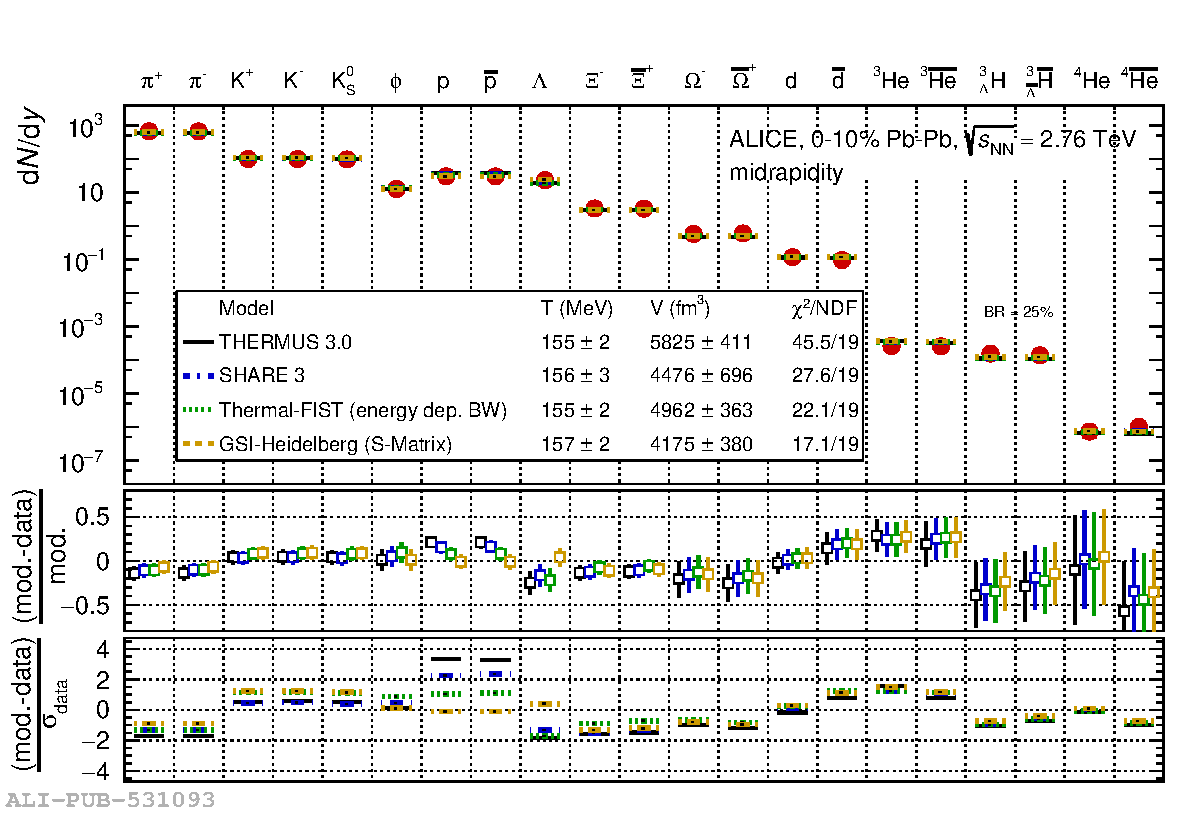
\includegraphics[width=\linewidth]{Figures/Chapter 1/SHM_fit_PbPb010_arp_all.pdf}
  \caption{Multiplicity per unit of rapidity of different hadron species and light nuclei measured by ALICE compared to SHM fits from THERMUS~\cite{Wheaton:2004qb}, SHARE~\cite{Torrieri:2004zz}, Thermal-FIST~\cite{Vovchenko:2019pjl}, and GSI-Heidelberg~\cite{Andronic:2005yp}. Differences between the model calculations and the measured yields are shown in the bottom panels. Figure taken from Ref.~\cite{ALICE:2022wpn}.}
  \label{fig:SHM_fit}
\end{figure}

\begin{sloppypar}
Figure~\ref{fig:SHM_fit} illustrates the yields of different identified hadron species measured by the ALICE Collaboration in the 10\% most central Pb--Pb collisions at \mbox{$\sqrt{s_\mathrm{NN}} = 5.02$~\tev}. They are compared to predictions from various implementations of the SHM, including THERMUS~\cite{Wheaton:2004qb}, GSI-Heidelberg~\cite{Andronic:2005yp}, SHARE~\cite{Torrieri:2004zz}, and Thermal-FIST~\cite{Vovchenko:2019pjl}. These models make different assumptions regarding the equilibrium condition and/or conservation laws at the chemical freeze-out stage. The SHM is capable of describing the different particle abundances, which span a large range of 9 orders of magnitude. The yields of exotic hadron species, such as hyperons and light nuclei are precisely described too. This confirms the assumption that the system is in thermal and chemical equilibrium at the time of the chemical freeze-out, and that the outcome of the hadronisation process is well described by a statistical approach.
\end{sloppypar}

The chemical freeze-out temperature is found to be of $\sim 155$~\mev, very close to that predicted by lattice QCD calculations for QCD phase transition. Most recent results from the ALICE Collaboration~\cite{ALICE:2023ulv} show that the measured electric charge and baryon chemical potentials at midrapidity at the LHC energies are compatible with 0, indicating that the system created in Pb--Pb collisions at the LHC is on average baryon free and electrically neutral.

\subsection{Radial flow}
After the chemical freeze-out, inelastic interactions between hadrons do not take place anymore. However, elastic interactions can still occur in the hadron gas, leading to a modification of the momentum distribution of the particles until the system reaches the thermal freeze-out. By studying the transverse momentum spectra of the particles produced in the collision, it is possible to extract information on the properties of the produced particles at the thermal freeze-out, and on the collective expansion (\emph{flow}) of the system.

For a stationary thermal source with a temperature $T$, the Lorentz-invariant momentum distribution of the particles is given by
\begin{equation*}
    E\frac{\de^3 N}{\de p^3} = \frac{\de^3 N}{\pt\de\pt\de\varphi\de y} = \frac{g_\mathrm{i}V}{(2\pi)^3} E \frac{1}{e^{(E-\mu_\mathrm{i})/T}\pm1}\quad ,
\end{equation*}
where $E$ is the energy of the particle, $g_\mathrm{i}$ and $\mu_\mathrm{i}$ are the degeneracy factor and chemical potential of the particles of species i, respectively, $V$ is the volume of the source, and the +1 term is for fermions while the $-1$ is for bosons. By using the relation
\begin{equation*}
  \frac{\de N}{\pt\de\pt} = \frac{\de N}{\mt\de\mt}\quad ,
\end{equation*}
and by assuming that $e^{(E-\mu_\mathrm{i})/T}\gg1$, the transverse momentum spectrum of particles can be obtained by integrating over the azimuthal angle $\varphi$ and the rapidity $y$, leading to
\begin{equation}\label{eq:mt_scaling}
    \frac{\de N}{\mt\de\mt} = \frac{g_\mathrm{i}V}{(2\pi)^2} \mt e^{\mu_\mathrm{i}/T} K_1\left(\frac{\mt}{T}\right) \xrightarrow[\mt\gg T]{} V'\sqrt{\mt}e^{-\mt/T}\quad .
\end{equation}
From Eq.~\ref{eq:mt_scaling} emerges that for a stationary thermal particle source with a temperature $T$, the transverse mass spectrum of the particles follows an exponential distribution with a slope parameter $T$, and is independent of the particle species. This is known as the \mt-scaling of the transverse mass spectra, and is observed in pp and small-system collisions at low \sqs, with a slope parameter of $T\sim167$~\mev~\cite{Heinz:2004qz}. However, in heavy-ion collisions, this description is not valid, as the QGP, which is a thermalised system of deconfined quarks and gluons, has a thermal pressure. The pressure difference between the QGP and the surrounding vacuum leads to a collective expansion of the fireball, which is called \emph{radial flow}. This causes the particles to be pushed in the transverse direction, causing a modification of the transverse momentum spectra of the particles, which is characterised by a shift of the spectra towards higher \pt values, with a more pronounced effect for heavier particles, as shown in Fig.~\ref{fig:RadialFlow}, where the \pt distributions measured by the ALICE Collaboration~\cite{ALICE:2022wpn} of different hadron species are shown for central (0--5\%) and peripheral (80--90\%) Pb--Pb collisions. The radial flow, as expected, is more pronounced in central collisions (due to the larger pressure gradients) which is manifest in the harder \pt spectra for central collisions as compared to peripheral ones. The radial flow is determined by a correlation between the velocity of an element of the system and its space-time position, which is superimposed on the random thermal motion of the particles.
\begin{figure}[t]
  \centering
  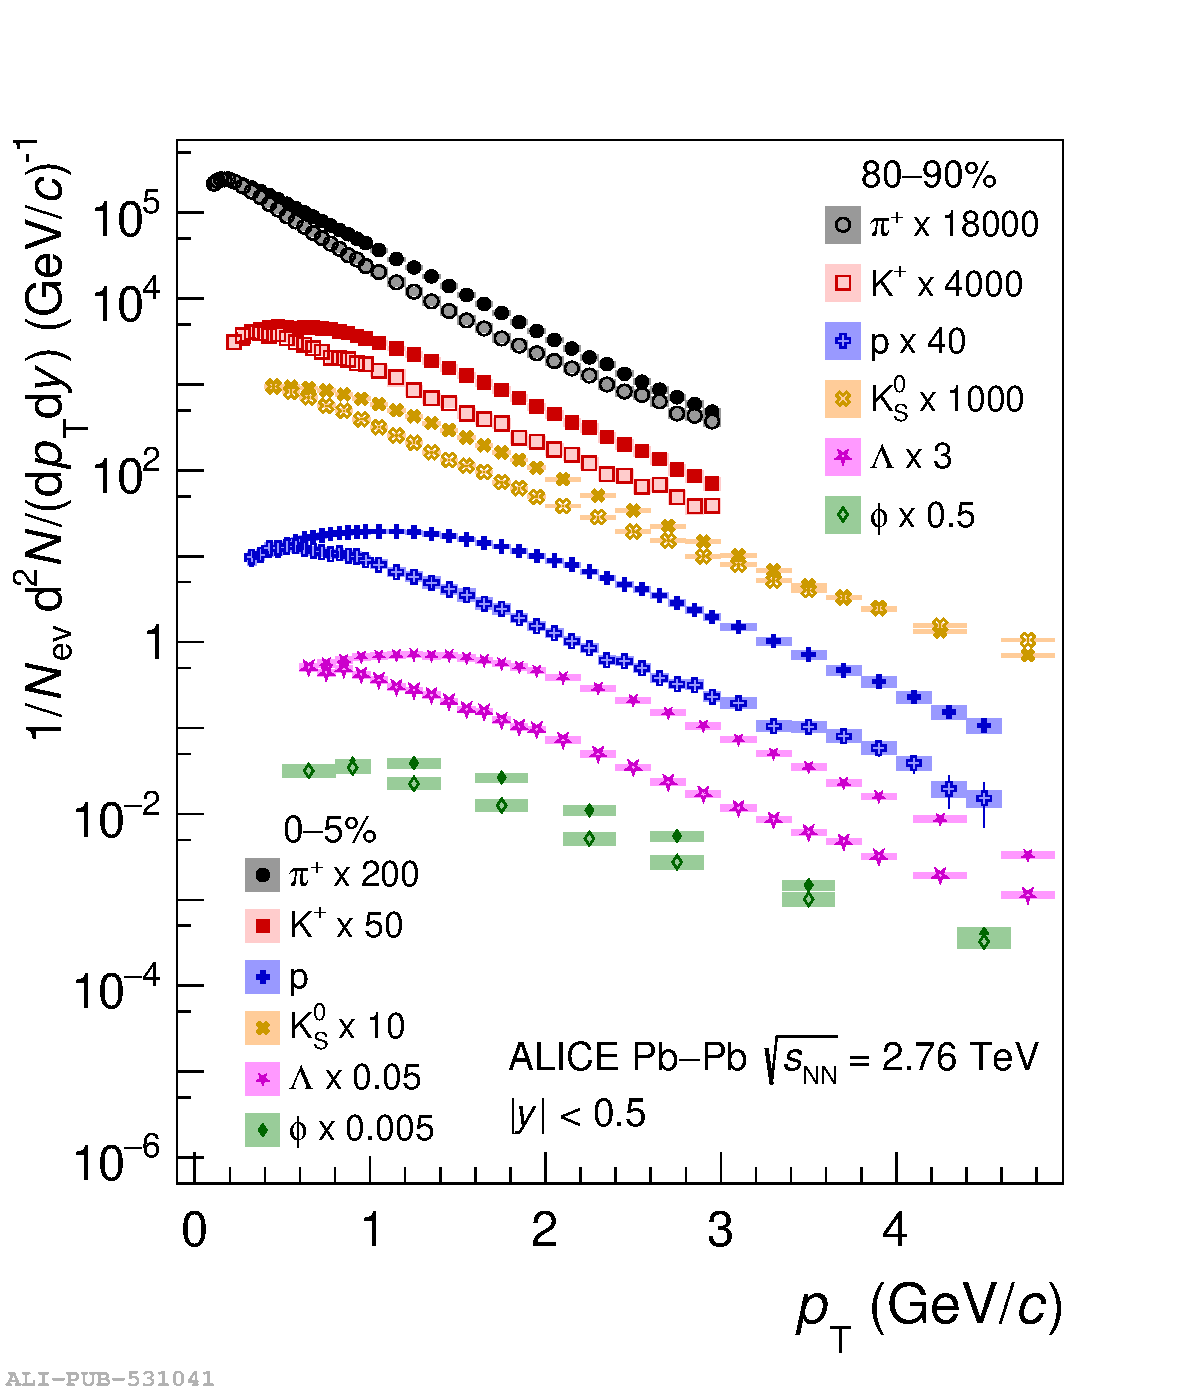
\includegraphics[width=0.7\linewidth]{Figures/Chapter 1/spectra_run1.pdf}
  \caption{Transverse momentum distributions of $\mathrm{\pi^+}$, $\mathrm{K^+}$, p, $\mathrm{K^0_s}$, $\mathrm{\Lambda}$, and $\mathrm{\phi}$ mesons for the 0--5\% and 80--90\% centrality intervals in Pb--Pb collisions at $\snn=2.76$~\tev measured by the ALICE Collaboration. The data points are scaled by various factors for better visibility. Figure taken from Ref.~\cite{ALICE:2022wpn}.}
  \label{fig:RadialFlow}
\end{figure}

\begin{figure}[htb]
  \centering
  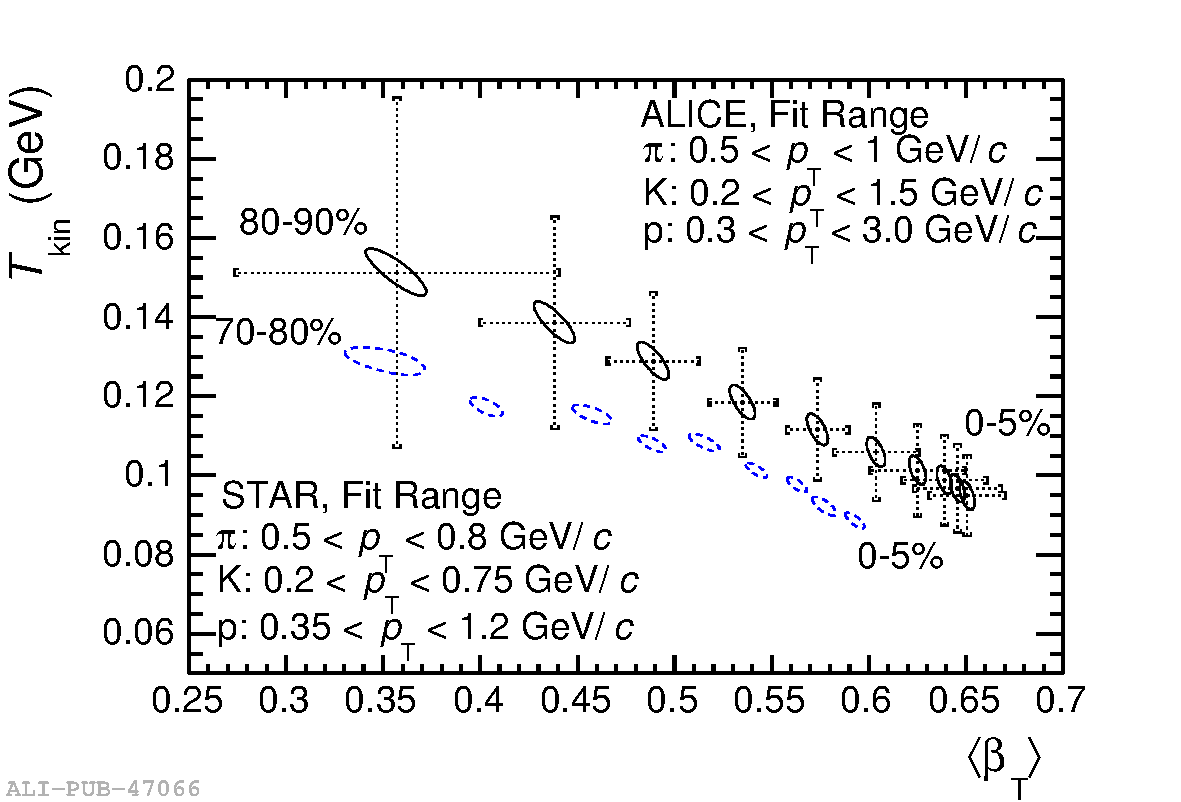
\includegraphics[width=0.7\linewidth]{Figures/Chapter 1/2014-Feb-27-cBlastWaveVsSTAR.pdf}
  \caption{Results of blast-wave fits obtained by the ALICE Collaboration at the LHC, compared to similar fits at RHIC energies from the STAR Collaboration, for different centrality intervals. Figure taken from Ref.~\cite{ALICE:2013mez}}
  \label{fig:blast_wave_fit}
\end{figure}

The radial flow can be described by using phenomenological models, such as the blast-wave model~\cite{Schnedermann:1993ws}, which assumes that the particles are emitted from a thermal source with a collective velocity field. It relies on the Cooper-Frye prescription~\cite{Cooper:1974mv}, which assumes an instantaneous freeze-out of the particles in the radial direction, to calculate the transverse momentum spectra of the particles in terms of the temperature of the source, the collective velocity field, and the transverse velocity profile. Results from SPS, RHIC, and LHC experiments show that the transverse momentum spectra of the particles produced in heavy-ion collisions can be well described by the blast-wave model, with a temperature of the source (which corresponds to the thermal freeze-out temperature $T_\mathrm{therm.}$) of around 110--120~\mev, almost independent of \snn, and a collective velocity field of around 0.5--0.6~$c$ in the most central collisions, with a growing trend with \snn, as shown in Fig.~\ref{fig:blast_wave_fit}.

Hydrodynamics-based models provided a more robust description of the system's expansion as compared to blast-wave fits. They rely on energy and momentum conservation laws, which need to be expressed in a relativistic form due to the relativistic nature of the system:
\begin{equation*}
    \partial_\mu T^{\mu\nu} = 0\quad ,~\mathrm{with}\quad T^{\mu\nu} = (\varepsilon + p)u^\mu u^\nu - p g^{\mu\nu}\quad ,
\end{equation*}
where $T^{\mu\nu}$ is the energy-momentum tensor, $\varepsilon$ is the energy density, $p$ is the pressure, $u^\mu$ is the four-velocity of the fluid element, and $g^{\mu\nu}$ is the metric tensor. An additional condition comes from the conservation of the baryon number, which is expressed as
\begin{equation*}
    \partial_\mu (n_B u^\mu) = 0\quad ,
\end{equation*}
where $n_B$ is the baryon density. A further equation is needed to close the system of equations, and is provided by the equation of state of the QGP, which relates the pressure to the energy density and the baryon density. As the fireball is in a non-equilibrium state in the early stages of the collision, the hydrodynamics equations need an initial condition to describe the system at the time $\tau_\mathrm{eq}$ in which it reaches the equilibrium and hydrodynamics can be applied. This is usually obtained via the Glauber~\cite{Miller:2007ri} or $\mathrm{T_RENTo}~\cite{Moreland:2014oya}$ models, which describe the collision of the two nuclei as a superposition of nucleon-nucleon collisions, and provide the initial energy density profile of the system. Models based on the Colour Glass Condensate framework such as IP-Glasma~\cite{Lappi:2006fp}, or Monte Carlo simulations based on the description of partonic showers such as AMPT~\cite{Lin:2004en} can also be used to provide the initial conditions for the hydrodynamics calculations. \\
The hydrodynamics calculations provide a good description of the transverse momentum spectra of the particles produced in heavy-ion collisions, and the emerging parameters (freeze-out temperature, flow velocity) are similar to those obtained with the blast-wave model. In addition, hydrodynamics calculations and their extensions, such as viscous hydrodynamics, can be used to study other observables related to the collective expansion of the system, such as the elliptic flow, which is a measure of the anisotropy of the particle emission in the transverse plane.

\subsection{\texorpdfstring{High-$p_\mathrm{T}$ hadrons and jet quenching}{High-pT hadrons and jet quenching}}\label{sec:high_pt}
\begin{figure}[htb]
  \centering
  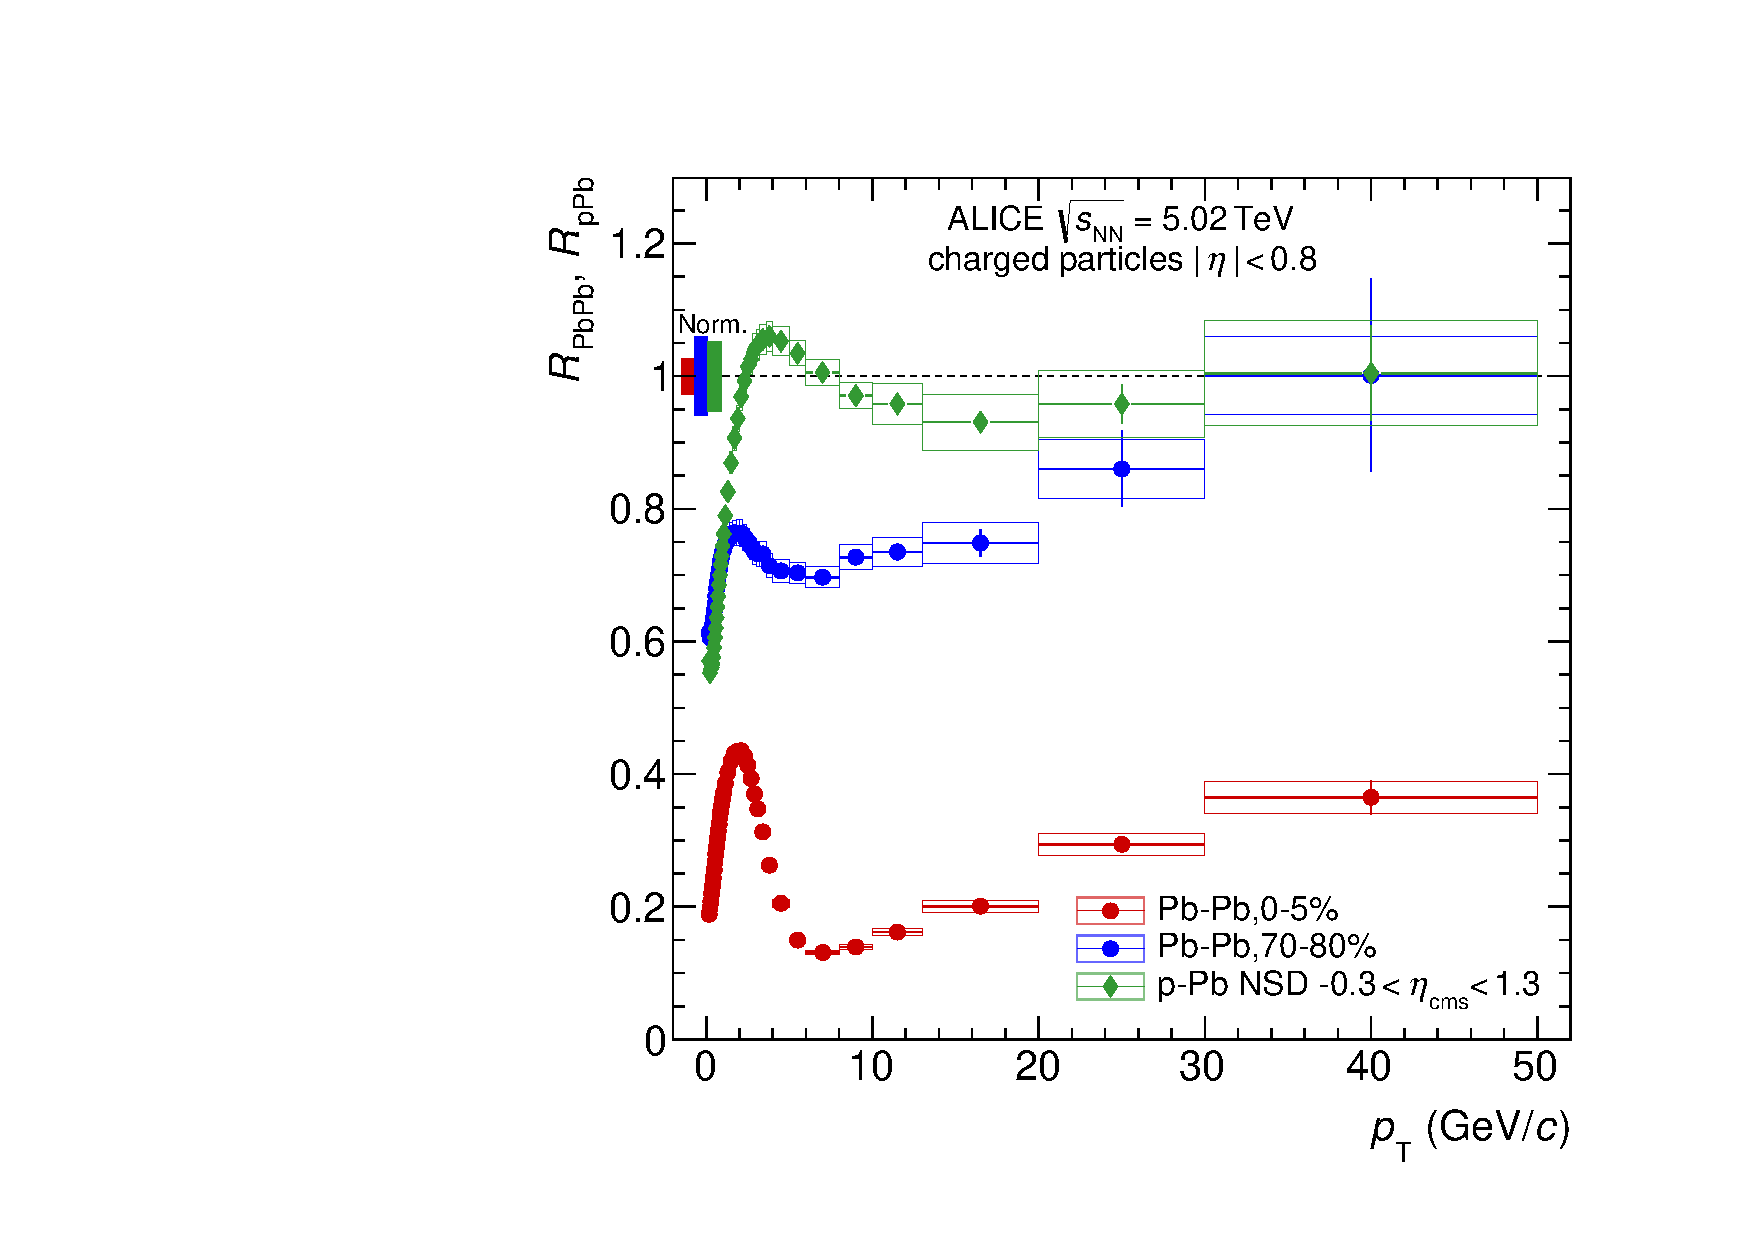
\includegraphics[width=0.7\linewidth]{Figures/Chapter 1/rAArpPb.pdf}
  \caption{Nuclear modification factors measured by ALICE in central $(0-5\%)$ and peripheral $(70-80\%)$ Pb--Pb collisions at $\snn=5.02$~\tev and in p--Pb collisions at $\snn = 5.02$~\tev. Figure taken from Ref.~\cite{ALICE:2018vuu}.}
  \label{fig:RAA}
\end{figure}

High-\pt partons are produced in hard-scattering processes, i.e., those with a high momentum transfer. As such, they are produced in the early stages of the collision and experience the whole fireball evolution. They can therefore be used to probe the properties of the earliest stages of the QGP. The Glauber model predicts the production cross-section of hard-scattering processes to scale with the number of binary nucleon-nucleon collisions. To test this prediction, the nuclear modification factor \raa is defined as the ratio of the \pt-differential hadron yield in heavy-ion collisions to the one in proton-proton collisions, scaled by the mean number of binary nucleon-nucleon collisions $\langle N_\mathrm{coll} \rangle$:
\begin{equation*}
    \raa = \frac{\de N_\mathrm{AA}/\de\pt}{\langle N_\mathrm{coll} \rangle~\de N_\mathrm{pp}/\de\pt}\quad .
\end{equation*}
The nuclear modification factor of particles produced in hard-scattering processes (jets, high \pt hadrons, heavy flavours) is expected to be equal to unity, namely \emph{binary scaling}, in the absence of nuclear effects. However, experimental results~\cite{ALICE:2018vuu} show that the \raa of charged particles measured in the most central heavy-ion collisions exhibits a suppression at low \pt, a peak at intermediate \pt ($\sim 2~\gevc$), and a significant suppression by a factor of $\sim5$ at high \pt, as shown in Fig.~\ref{fig:RAA}. The suppression at low \pt and the peak at intermediate \pt are mostly attributed to soft particle production, which dominates at low \pt and does not scale with $N_\mathrm{coll}$. In addition, other initial-state effects, such as the modification of parton distribution functions in the nucleus~\cite{Arneodo:1992wf}, and the Cronin effect~\cite{Kopeliovich:2002yh} modify the spectra in Pb--Pb (and p--Pb) collisions as compared to pp. In addition, the radial flow causes a modification of the spectral shapes at low \pt and affects the \raa. The initial-state effects can be studied in small collision systems~\cite{PHENIX:2021dod}, where the production of a QGP is not expected, or through the measurement of the \raa for colour-neutral particles, such as photons~\cite{PHENIX:2012jbv}, which are not affected by the presence of a deconfined medium. The high-\pt suppression of \raa increases with collision centrality and is related to the formation of the QGP. Partons traversing the medium lose energy through elastic scatterings with the QGP constituents and via gluon radiation, which is the dominant process for high-energy partons. This energy loss can be described in the BDMPS formalism~\cite{Baier:1996kr}, which assumes that the radiated gluon becomes de-coherent from the emitting parton through multiple soft scatterings with the medium constituents. The energy loss of the partons is quantified as
\begin{equation*}
    \Delta E = \frac{1}{4}\alpha_s C_\mathrm{R}\hat{q}L^2\quad ,
\end{equation*}
Where \als is the strong coupling constant, $C_\mathrm{R}$ is the Casimir factor, which is 3 for gluon-gluon couplings and 4/3 for quark-gluon interactions, $\hat{q}$ is the transport coefficient, and $L$ is the path length of the parton in the medium. The transport coefficient is related to the energy density of the medium, as $\hat{q} \propto \varepsilon^{3/4}$~\cite{Baier:2002tc}, so that energy loss measurements can be used to infer the properties of the QGP. Typical energy losses of high-\pt partons traversing the whole QGP are of the order of 40~\gev, which is a significant fraction of the parton energy. The energy loss of the partons leads to a suppression of high-\pt hadron yield, which consequently leads to a suppression of the nuclear modification factor at high \pt. 

\begin{figure}[htb]
  \centering
  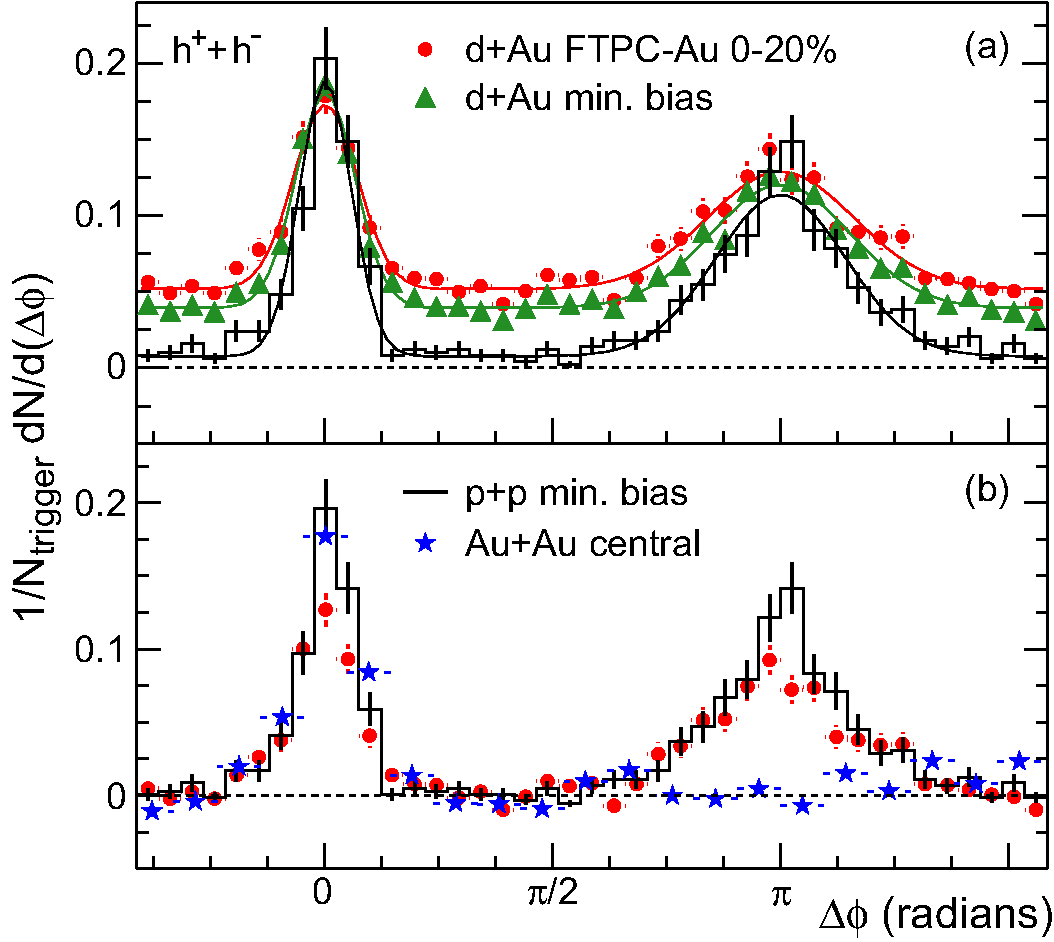
\includegraphics[width=0.7\linewidth]{Figures/Chapter 1/dAu_Fig4.pdf}
  \caption{Top: Two-particle azimuthal correlations for minimum bias and central d--Au collisions, and for proton-proton collisions at $\snn = 200$~\gev measured by the STAR Collaboration. Bottom: Comparison of pedestal-subtracted two-particle azimuthal correlations for central Au--Au collisions to those seen in proton-proton collisions. Figure taken from Ref.~\cite{STAR:2003pjh}.}
  \label{fig:azimuthal_correlations}
\end{figure}

At leading order, partons are produced in back-to-back pairs, forming what are known as di-jets. In the presence of the QGP, the jets are expected to be modified due to the interactions with the medium, an effect known as \emph{jet quenching}. For example, the opening angle of the jets is observed to be broadened~\cite{ALICE:2015tra}, and the \pt distribution of the leading hadron (i.e., the one with the highest \pt) is expected to be softer than that measured in pp collisions~\cite{ATLAS:2017xfa}, therefore yielding an \raa smaller than unity at high \pt. 

Further insights into the jet quenching mechanism can be obtained by measuring two-particle azimuthal correlations. For each event, the particle with the highest \pt above a certain threshold is selected as the trigger particle, and the azimuthal angle of other high-\pt particles is measured with respect to the first one. For proton-proton and proton-nucleus collisions, the azimuthal distribution presents two peaks: the \emph{near-side peak}, which is found at $\varphi=0$ and is due to the hadrons produced in the same jet as the trigger particle, and the \emph{away-side peak}, which is found at $\varphi=\pi$ and is due to the hadrons produced in the opposite jet. In heavy-ion collisions, the away-side peak is suppressed due to the energy loss in the QGP, as shown in Fig.~\ref{fig:azimuthal_correlations}. In fact, for a di-jet surface emission, the parton shower generated by the jet pointing in the direction of the medium is expected to lose more energy than the one pointing in the opposite direction, yielding the suppression of the away-side peak.

%In addition, the QGP can also affect the hadronisation process. In small collision systems, such as pp and p--Pb collisions, hadronisation occurs via fragmentation, where the colour string holding together a quark-antiquark pair breaks, producing another quark-antiquark pair. This process leads to the production of a collimated jet of hadrons with \pt lower than the one of the first quark-antiquark pair. When the QGP is produced, another hadronisation mechanism becomes available, as the QGP is a thermalised system: the coalescence (or recombination) mechanism. Low \pt partons close in the velocity-space phase space can bind together to form a higher-\pt hadron. This enhances the production of baryons, as the \pt-distribution of partons inside the QGP follows a rapidly decreasing trend.

\subsection{Strangenness enhancement}\label{subsec:StrangenessEnhancement}
One of the first proposed signatures of the QGP formation is the strangeness enhancement~\cite{Rafelski:1982pu}, which refers to the observation of an increased production of strange hadrons in heavy-ion collisions compared to proton-proton collisions. At a microscopic level, the enhancement of strange hadrons is a direct consequence of the high temperatures reached in the QGP, which allow for the thermal production of strange quarks and antiquarks. Strange quarks are not present as valence quarks in the initial state, and can be produced in hard $2\rightarrow 2$ scatterings ($gg\rightarrow s\overline{s},~q\overline{q}\rightarrow s\overline{s}$), or via gluon splitting ($g\rightarrow s\overline{s}$) during the evolution of the system. While these processes are dominant for the production of strange hadrons with high \pt, at low \pt the production of strangeness is dominated by non-perturbative processes. At a macroscopic level, the enhancement of the production of strange hadrons in the presence of QGP can be explained using the statistical approach of the SHM. The description of hadron production in smaller colliding systems, such as $\mathrm{e^+e^-}$ and pp collisions, requires the use of a canonical ensemble, which is used to describe a system that exchanges only energy with a reservoir, and requires the exact (local) conservation of quantum numbers. This reduces the phase space available for strange particle production~\cite{Redlich:2001kb}, leading to a suppression of strange quark production as compared to the grand canonical ensemble, called \emph{canonical suppression}. 

The strangeness enhancement in heavy-ion collisions has been observed by several Collaborations, such as the WA97~\cite{WA97:1999uwz} and NA57~\cite{NA57:2010tnk} at the SPS, STAR at RHIC~\cite{STAR:2007cqw}, and ALICE at the LHC~\cite{ALICE:2013xmt}. In addition, an enhancement of strange hadrons has been observed in small systems, such as pp~\cite{ALICE:2016fzo} and p-Pb~\cite{ALICE:2013wgn, ALICE:2015mpp} collisions, in high-multiplicity events, and follows a hierarchy determined by the hadron strangeness. This observation is intriguing, as QGP production is not expected in such systems. Furthermore, several effects such as azimuthal correlations and mass-dependent hardening of \pt distributions, which are typically associated with QGP formation in nuclear collisions, have been observed in these systems. Could small droplets of QGP be formed in these collisions? Could other mechanisms explain the observed effects? These are still open questions in the field of high-energy nuclear physics, and they are the subjects of ongoing research.

\begin{figure}[htb]
  \centering
  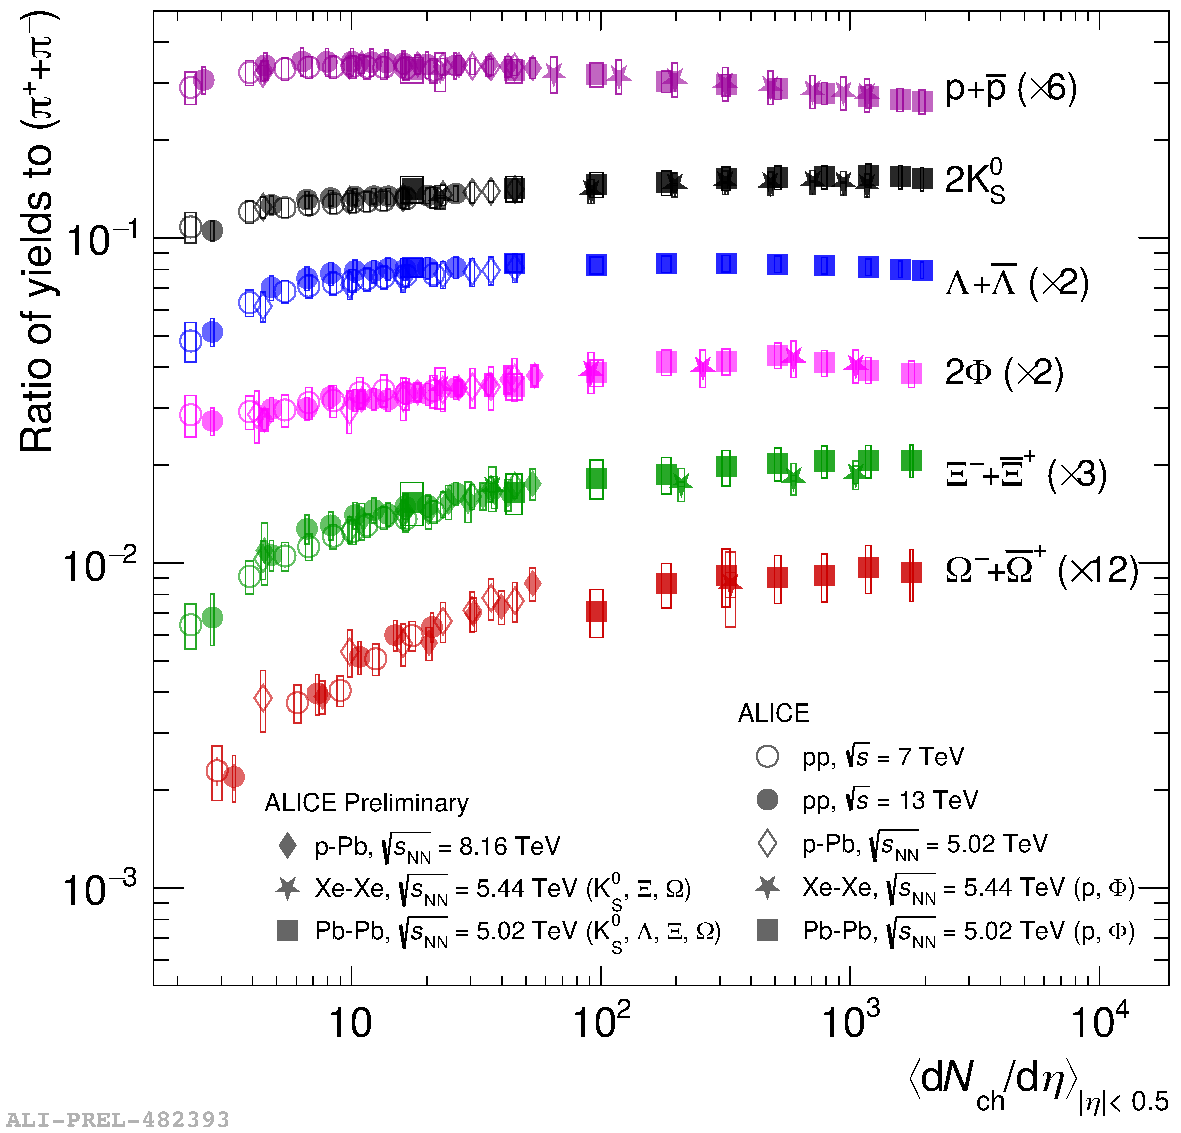
\includegraphics[width=0.7\linewidth]{Figures/Chapter 1/img_ToPionRatios_1.pdf}
  \caption{\pt--integrated yield ratios of strange (\kzs, $\Lambda$) and multi-strange ($\Xi^\pm, \Omega^\pm$) hadrons to pions ($\pi^++\pi^-$) as a function of $\braket{\de N_\mathrm{ch}/\de\eta}$ measured in pp, p--Pb and Pb--Pb collisions at midrapidity$(\lvert y\rvert<0.5)$. Figure taken from Ref.~\cite{ALICE_figures}.}
  \label{fig:StrangenessEnhancement}
\end{figure}

Figure~\ref{fig:StrangenessEnhancement} shows the \pt-integrated yield ratios of strange (\kzs, $\Lambda$) and multi-strange ($\Xi^\pm, \Omega^\pm$) hadrons to pions ($\pi^++\pi^-$) as a function of the charged particle multiplicity density, $\braket{\de N_\mathrm{ch}/\de\eta}$, measured in $\lvert y\rvert<0.5$ in different collision systems (pp, p--Pb and Pb--Pb) by the ALICE Collaboration at the LHC~\cite{ALICE:2016fzo}. The data show a clear enhancement of strange to non-strange hadron production with a smooth trend with increasing multiplicity. At the highest multiplicities of Pb--Pb collisions, the yield ratios saturate at values that are described by SHM calculations with a grand canonical ensemble. This can be interpreted as a consequence of the formation of a QGP in Pb-Pb collisions, where the $\mathrm{s\overline{s}}$ is expected to rapidly reach its equilibrium value.


%In the QGP, strange quarks are produced through the interactions between the quarks and gluons, and they can form strange hadrons, such as the $\Lambda$, $\Xi$, and $\Omega$ baryons. The production of strange hadrons in heavy-ion collisions is a key signature of the QGP, and it has been observed in several experiments, such as the ALICE experiment at the LHC~\cite{ALICE:2022wpn}. The strangeness enhancement is a direct consequence of the high energy densities reached in the collisions, which allow for the production of strange quarks and antiquarks. In the QGP, strange quarks are produced through the interactions between the quarks and gluons, and they can form strange hadrons, such as the $\Lambda$, $\Xi$, and $\Omega$ baryons. The production of strange hadrons in heavy-ion collisions is a key signature of the QGP, and it has been observed in several experiments, such as the ALICE experiment at the LHC~\cite{ALICE:2022wpn}.
\setcounter{chapter}{1}
%\chapter{Open heavy-flavour production in proton-proton collisions}\label{ch:openHF}

Open heavy-flavour hadrons, composed of a heavy quark (charm or beauty) along with lighter quarks, are exclusively formed in high-momentum transfer processes due to the large masses of approximately 1.3 \gevcc and 4.2 \gevcc~\cite{pdg} for charm and beauty quarks, respectively. As a result, heavy quarks are created in the early stages of the collision, and their production cross-section in the partonic interaction can be evaluated perturbatively using QCD. Studying the production of open heavy-flavour hadrons in proton-proton (pp) collisions not only provides a crucial test of the perturbative QCD framework, but also allows to set constraints on heavy-quark hadronisation models. Furthermore, measurements in proton-proton collisions, where the production of an extended deconfined medium is not expected, are a necessary reference for the study of heavy-ion collisions, where the properties of the QGP can be investigated. 

\section{Factorisation theorem}
The production of open heavy-flavour hadrons in proton-proton collisions can be described using the factorisation theorem~\cite{Collins:1989gx}, which allows for the separation of short-distance, perturbative behaviour from long-distance, non-perturbative phenomena. The total production cross-section can be expressed as
\begin{equation}\label{eq:pp_xsec}
    \sigma_{\text{pp}}^\mathrm{H} = \sum_\mathrm{a,b = g, q, \overline{q}} \int \de x_1 \de x_2 f_\mathrm{a/A}(x_1,\mu_\mathrm{F}^2) f_\mathrm{b/B}(x_2,\mu_\mathrm{F}^2) \hat{\sigma}_\mathrm{ab \rightarrow Q\overline{Q}} (x_1,x_2,\mu_\mathrm{F}^2,\mu_\mathrm{R}^2) D_\mathrm{Q\rightarrow H_Q}(z,\mu_\mathrm{F}^2) \quad ,
\end{equation}
i.e., the convolution of: i) the Parton Distribution Functions (PDFs) $f_\mathrm{a/A}(x_1,\mu_\mathrm{F}^2)$ and $f_\mathrm{b/B}(x_2,\mu_\mathrm{F}^2)$, describing the initial-state probability of finding a parton a in the proton A carrying a fraction $x_1$ of the proton's momentum, and a parton b in the proton B carrying a fraction $x_2$ of its momentum, respectively; ii) the hard partonic scattering cross-section $\hat{\sigma}_\mathrm{ab \rightarrow Q\overline{Q}} (x_1,x_2,\mu_\mathrm{F}^2,\mu_\mathrm{R}^2)$, defining the probability of producing the $\mathrm{Q\overline{Q}}$ final state from the collision of partons a and b, where Q is either a charm or beauty quark; and iii) the Fragmentation Functions (FFs) $D_\mathrm{Q\rightarrow H_Q}(z,\mu_\mathrm{F}^2)$, which describe the probability of the heavy quark Q to fragment into a heavy-flavour hadron $\mathrm{H_Q}$ carrying a fraction of the parent parton momentum $z$. $\mu_\mathrm{F}$ and $\mu_\mathrm{R}$ are the factorisation and renormalisation scales, respectively. The former is the scale at which the non-perturbative processes are separated from the perturbative ones, while the latter is the scale at which the ultraviolet divergences, emerging from the calculations of scattering amplitudes involving loop diagrams, are subtracted. While the PDFs and FFs are non-perturbative quantities, parametrised from experimental data and regarded as universal across different collision systems, the hard partonic scattering cross-section can be perturbatively calculated using QCD, but needs specific evaluations for each process. 

The factorisation theorem has been widely employed to describe the production of open heavy-flavour hadrons in proton-proton collisions, and has proven to be successful in modeling experimental data. Figure~\ref{fig:ppDmeson} shows the production cross-section of prompt and non-prompt $\mathrm{D^0}$-mesons in proton-proton collisions at $\sqrt{s} = 5.02$~\tev measured at midrapidity ($\lvert y\rvert<0.5$) as a function of the transverse momentum (\pt) by the ALICE Collaboration~\cite{ALICE:2021mgk}, compared to Fixed-Order plus Next-to-Leading Logarithms (FONLL) perturbative QCD predictions~\cite{Cacciari:1998it} combined with the \textsc{Pythia}~8~\cite{Sjostrand:2014zea} event generator for the $\mathrm{H_b \rightarrow D^0+X}$ decay kinematics. The calculation is performed at next-to-leading order, including all the $\als^2$ and $\als^3$ terms, with the resummation of the next-to-leading logarithmic terms. These include terms of the form $\alpha_s^2\alpha_s^k\log^k(\pt/m)$ and $\alpha_s^3\alpha_s^k\log^k(\pt/m)$, where $m$ is the heavy-quark mass. The term \emph{prompt} refers to charm-hadrons directly produced in the hadronisation of a charm quark or through the strong decay of a directly produced excited charm-hadron or charmonium state, while \emph{non-prompt} charm hadrons are produced in the decay of a hadron containing a beauty quark. The FONLL predictions are in good agreement with the non-prompt $\mathrm{D^0}$-meson production cross-section, whereas the prompt contribution lies at the upper edge of the theoretical uncertainty band, albeit being described within the uncertainties. Similar trends are observed in the production of other open heavy-flavour hadrons across different experimental facilities, such as the Tevatron~\cite{CDF:2003vmf}, RHIC~\cite{STAR:2012nbd}, and LHC~\cite{ALICE:2021mgk}.

\begin{figure}[htb]
    \centering
    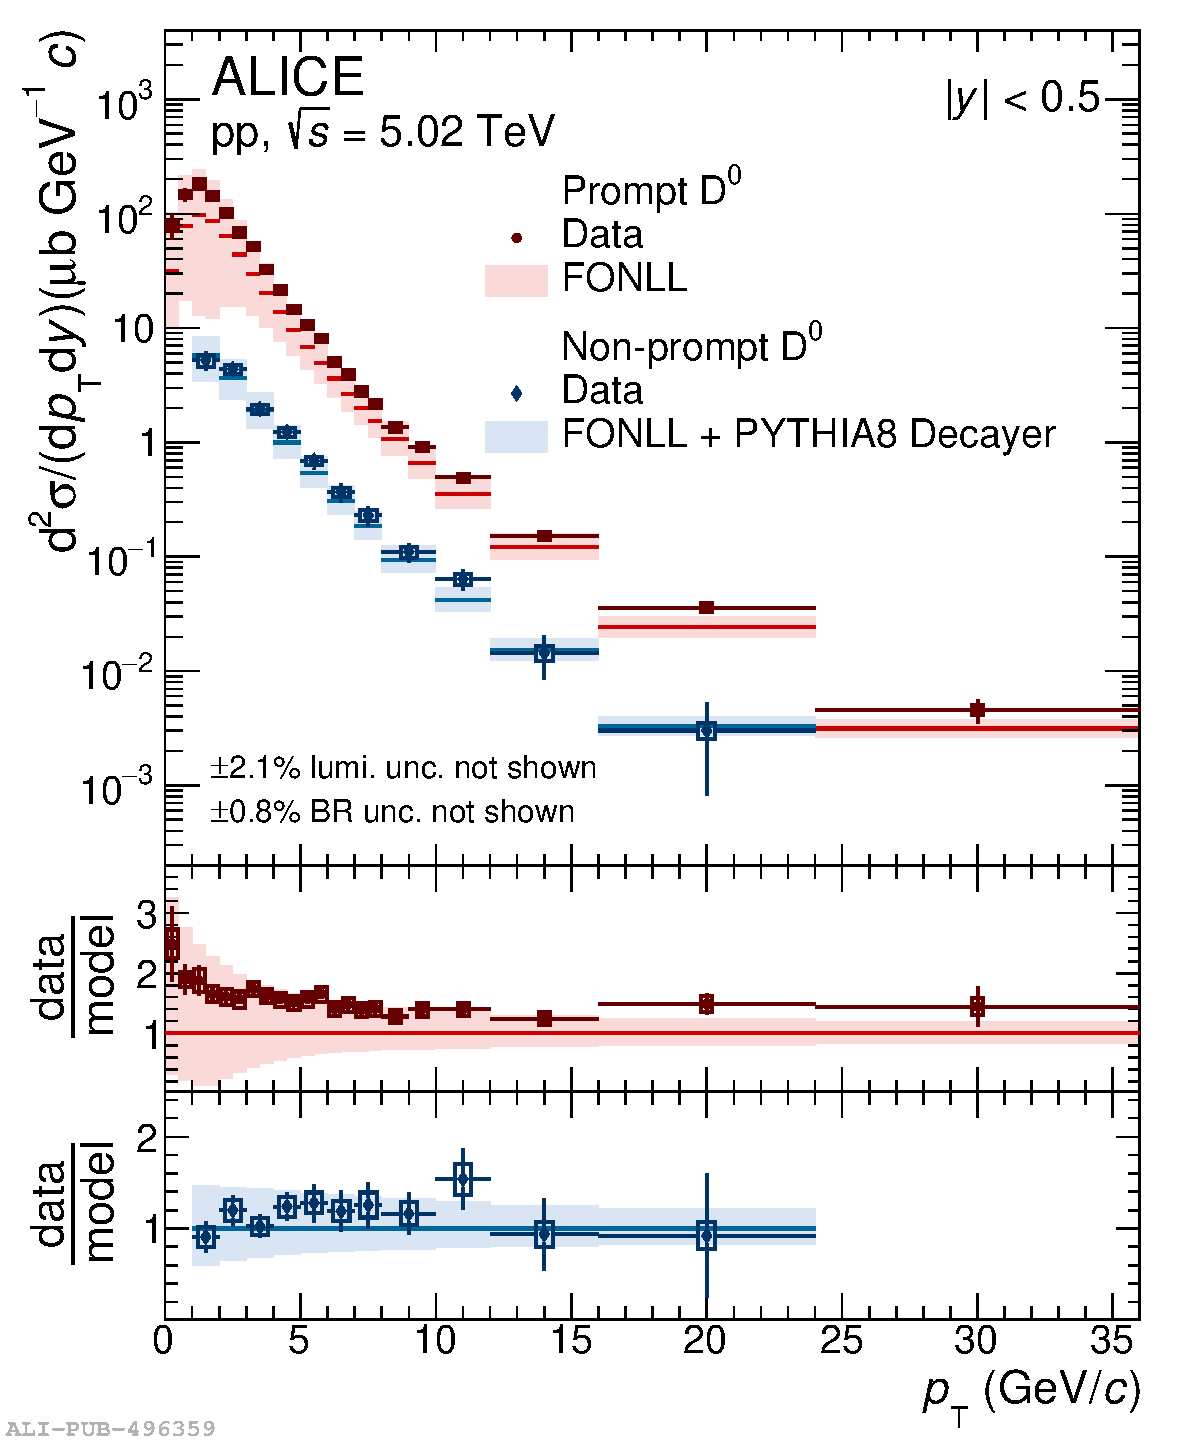
\includegraphics[width=0.6\linewidth]{Figures/Chapter 2/CrossSectionD0_Prompt_NonPrompt_pp5TeV_vsFONLL_Pythia8_BRnative_1.pdf}
    \caption{\pt-differential production cross-section of prompt and non-prompt $\mathrm{D^0}$-mesons measured at midrapidity ($\lvert y\rvert<0.5$) in pp collisions by the ALICE Collaboration at $\sqs=5.02$~\tev~\cite{ALICE:2021mgk} compared to predictions obtained with FONLL calculations~\cite{Cacciari:1998it} combined with \textsc{Pythia}~8~\cite{Sjostrand:2014zea} for the $\mathrm{H_b \rightarrow D^0+X}$ decay kinematics. Figure taken from Ref.~\cite{ALICE:2021mgk}}
    \label{fig:ppDmeson}
\end{figure}

\subsection{Parton Distribution Functions}
\subsubsection{Deep inelastic scattering}
The PDFs are non-perturbative quantities describing the probability of finding a parton carrying a fraction $x$ of the proton's momentum in the initial state of a process. The first experimental evidence revealing the partonic structure of the proton emerged from deep inelastic scattering experiments carried out at the Stanford Linear Accelerator Center (SLAC) in the 1960s~\cite{Friedman:1972sy}, where an electron was scattered off a proton with momentum $P$
, and the transferred momentum $q$ was measured. The cross-section for deep inelastic scattering can be defined in terms of the Lorentz invariant variables $Q^2 = -q^2$ and $x = \frac{Q^2}{2P\cdot q}$, yielding
\begin{equation*}
    \frac{\de^2\sigma}{\de x \de Q^2} = \frac{4\pi\alpha^2}{xQ^4} \left[ \left(1-y\right)F_2(x,Q^2) - xy^2F_1(x,Q^2) \right]\quad ,
\end{equation*}
where $y=Q^2/(sx)$, $s = (P+p_\mathrm{e})^2$ denotes the centre-of-mass energy of the electron-proton system, and the structure functions $F_1(x,Q^2)$ and $F_2(x,Q^2)$ represent an extension of the form factors for elastic scattering.
The first measurements of high-energy inclusive inelastic scattering experiments were performed using a 20~GeV linear accelerator at SLAC, and showed that the structure functions $F_1(x,Q^2)$ and $F_2(x,Q^2)$ were independent of $Q^2$ at fixed $x$ within the studied $1<~Q^2~<~10$~\gevcc range. This was in contrast with the behavior observed for the proton elastic form factors, where a decrease of two orders of magnitude was observed within the same $Q^2$ interval. This independence of the structure functions from $Q^2$ in deep inelastic scatterings was predicted by Bjorken in 1968 for $Q^2 \rightarrow \infty$~\cite{Bjorken:1968dy}, and is known as \emph{Bjorken scaling}. A physical interpretation of this phenomenon arrived just one year later, in 1969, with Feynman's parton model~\cite{Feynman:1969ej}, which described the interaction in terms of elastic scattering of the probe off a point-like constituent (parton) within the proton. This model explains the scale-invariance property of the proton structure functions, as the scattering centres are assumed to be structure-less. In this picture, the Bjorken variable $x$ acquires a new interpretation as the fraction of the proton momentum carried by the struck parton. The parton model also offers a straightforward definition of the structure functions in terms of the parton distribution functions $f_\mathrm{a}(x)$:
\begin{equation*}
    F_2(x,Q^2) = \sum_\mathrm{a} e_\mathrm{a}^2 x f_\mathrm{a}(x)\quad ,
\end{equation*}
where the sum is over partons with electric charge $e_\mathrm{a}$, and $f_\mathrm{a}$ are unknown, but universal functions for a given hadron, describing the probability of finding a parton of type a with a fraction $x$ of the proton's momentum. 

To explore the spin properties of the partons, the structure functions $F_1$ and $F_2$ were studied at different centre-of-mass energies. By investigating the relationship between the two structure functions, it was established that the partons have spin 1/2, as the Callan-Gross relation~\cite{Callan:1969uq}, which holds true for point-like Dirac particles, was found to be satisfied:
\begin{equation*}
    F_2(x,Q^2) = 2x F_1(x,Q^2)\quad .
\end{equation*}

In the next years, it became clear that additional constituents within the proton carry momentum but lack electric or weak charge, as the so-called momentum sum rule was not saturated by the measured PDFs in electron and neutrino scatterings. This missing momentum was attributed to gluons, which were discovered in the 1970s and are the field quanta of the strong force.

\subsubsection{Bjorken scaling violation}
\begin{figure}[htb]
    \centering
    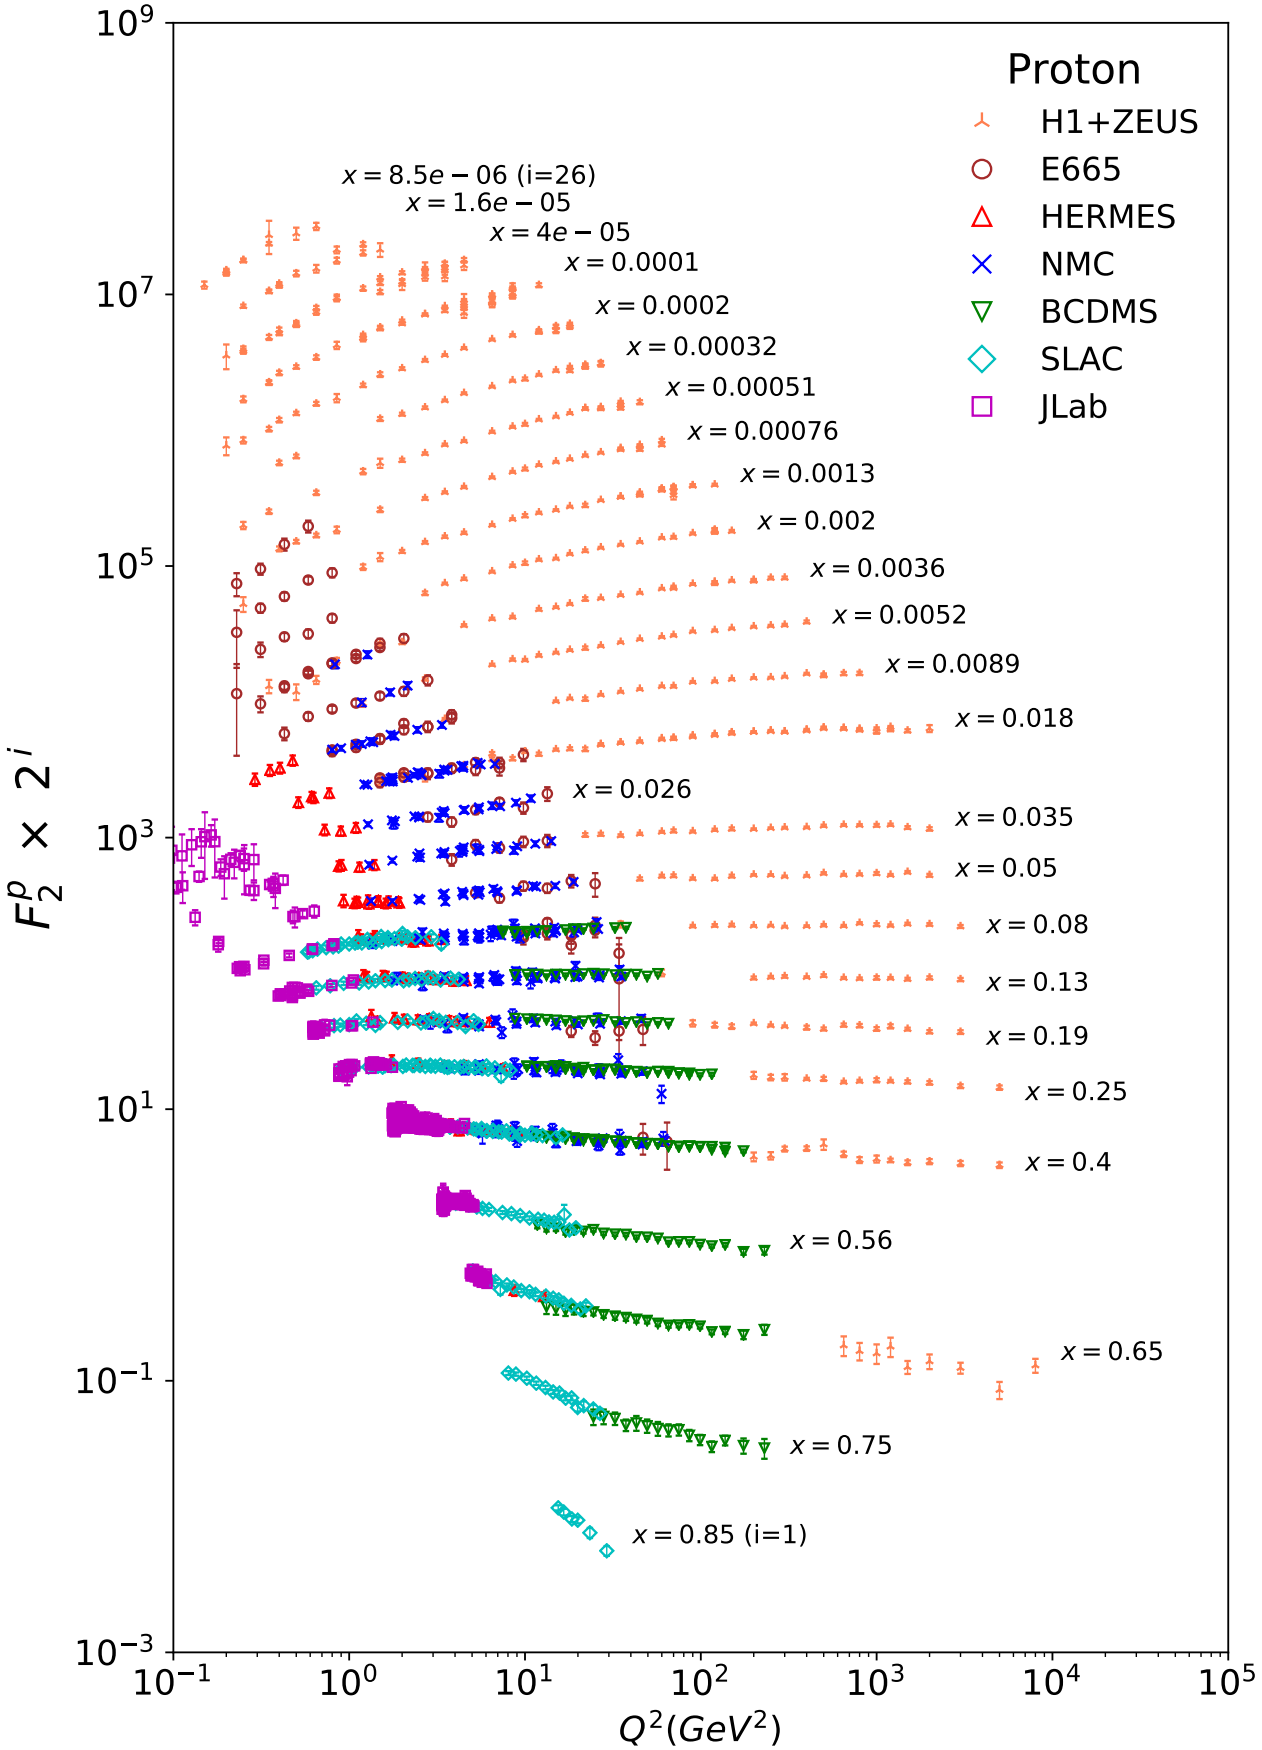
\includegraphics[width=0.6\linewidth]{Figures/Chapter 2/F2Results.png}
    \caption{The proton structure function $F^p_2$ measured in electromagnetic scattering of electrons and positrons on protons, and for electrons/positrons and muons on a fixed target~\cite{pdg}.}
    \label{fig:scaling_violation}
\end{figure}
By the late 1970s, measurements of the structure functions at larger $Q^2$ values taken at CERN and DESY revealed that Bjorken scaling was violated, i.e., the structure functions were not $Q^2$ independent. Figure~\ref{fig:scaling_violation} shows measurements of the proton structure functions $F_2(x,Q^2)$ as a function of $Q^2$ for various values of $x$ taken from different experiments~\cite{pdg}. It is clear from the plot that structure functions present an increasing trend as a function of $Q^2$ at low $x$, and a decreasing trend as a function of $Q^2$ at high $x$. 

The parton model fails to explain this behaviour, as it relies on the assumption that the transferred energy is sufficiently large to neglect the proton and its constituents' masses, as well as the interactions among partons. In particular, the partons' transverse momentum with respect to the proton momentum is neglected. The key to understanding Bjorken scaling violation comes from QCD and the realisation that the parton's transverse momentum is not necessarily restricted to be small. A quark, for instance, can emit a gluon and acquire large transverse momentum $k_T$ with a probability proportional to $\als \de k_T/k_T^2$ at large $k_T$. The integral extends up to the kinematic limit $k_T\sim Q^2$, giving rise to contributions proportional to $\als\mathrm{log}Q^2$, which break the scaling. The evolution of PDFs with $Q^2$ from a parametrisation at a given $Q^2_0$ can be perturbatively described using the Dokshitzer-Gribov-Lipatov-Altarelli-Parisi (DGLAP) evolution equations~\cite{Gribov:1972ri,Dokshitzer:1977sg,Altarelli:1977zs}, which require the introduction of a new arbitrary scale, at which the factorisation of the non-perturbative processes happens: the factorisation scale $\mu_\mathrm{F}$. There exists a wide range of PDF parametrisations, such as the NNPDF~\cite{NNPDF:2021njg}, CTEQ~\cite{Dulat:2015mca}, and MMHT~\cite{Harland-Lang:2014zoa}, which are determined from global fits to a wide range of experimental data, including deep inelastic scattering, Drell-Yan, and jet production.
\subsection{Partonic cross-section}\label{sec:partonic_cross_section}
\begin{figure}[htb]
    \centering
    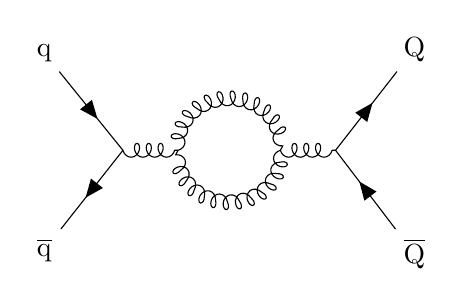
\begin{tikzpicture}
      \begin{feynman}
        \vertex (a);
        \vertex [above=1cm of a] (b) {q};
        \vertex[below=1cm of a] (c) {$\overline{\mathrm{q}}$};
        \vertex[right=1cm of a] (d);
        \vertex[right=0.7cm of d] (e);
        \vertex[right=1.3cm of e] (f);
        \vertex[right=0.7cm of f] (g);
        \vertex[right=1cm of g] (h);
        \vertex[above=1cm of h] (i) {Q};
        \vertex[below=1cm of h] (j) {$\overline{\mathrm{Q}}$};
        \diagram* {
            (b) -- [fermion] (d) -- [fermion] (c),
            (d) -- [gluon] (e),
            (e) -- [gluon,  in=90, out=90, looseness=1.7] (f) -- [gluon,  in=-90, out=-90, looseness=1.7] (e),
            (f) -- [gluon] (g),
            (j) -- [fermion] (g) -- [fermion] (i),
        };
      \end{feynman}
    \end{tikzpicture}\quad
    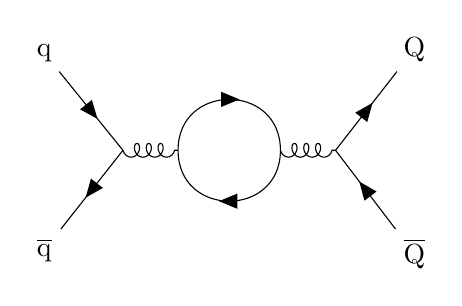
\begin{tikzpicture}
        \begin{feynman}
          \vertex (a);
          \vertex [above=1cm of a] (b) {q};
          \vertex[below=1cm of a] (c) {$\overline{\mathrm{q}}$};
          \vertex[right=1cm of a] (d);
          \vertex[right=0.7cm of d] (e);
          \vertex[right=1.3cm of e] (f);
          \vertex[right=0.7cm of f] (g);
          \vertex[right=1cm of g] (h);
          \vertex[above=1cm of h] (i) {Q};
          \vertex[below=1cm of h] (j) {$\overline{\mathrm{Q}}$};
          \diagram* {
              (b) -- [fermion] (d) -- [fermion] (c),
              (d) -- [gluon] (e),
              (e) -- [fermion,  in=90, out=90, looseness=1.7] (f) -- [fermion,  in=-90, out=-90, looseness=1.7] (e),
              (f) -- [gluon] (g),
              (j) -- [fermion] (g) -- [fermion] (i),
          };
        \end{feynman}
      \end{tikzpicture}

    \vspace*{0.5cm}
    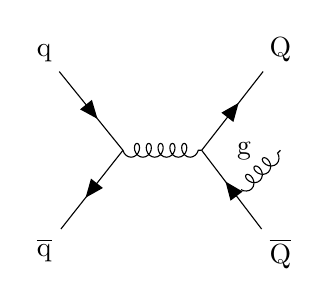
\begin{tikzpicture}
        \begin{feynman}
          \vertex (a);
          \vertex [above=1cm of a] (b) {q};
          \vertex[below=1cm of a] (c) {$\overline{\mathrm{q}}$};
          \vertex[right=1cm of a] (d);
          \vertex[right=1cm of d] (e);
          \vertex[right=1cm of e] (f);
          \vertex[above=1cm of f] (g) {Q};
          \vertex[below=1cm of f] (h) {$\overline{\mathrm{Q}}$};
          \vertex[right=0.5cm of e] (i);
          \vertex[below=0.5cm of i] (j);
          \diagram* {
              (b) -- [fermion] (d) -- [fermion] (c),
              (d) -- [gluon] (e),
              (h) -- [fermion] (e) -- [fermion] (g),
              (j) -- [gluon, edge label = g] (f),

          };
        \end{feynman}
      \end{tikzpicture}\quad
      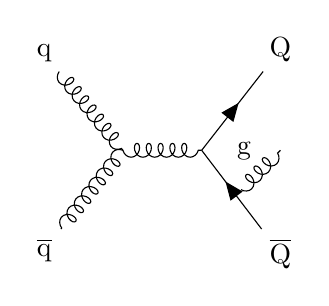
\begin{tikzpicture}
        \begin{feynman}
            \vertex (a);
            \vertex [above=1cm of a] (b) {q};
            \vertex[below=1cm of a] (c) {$\overline{\mathrm{q}}$};
            \vertex[right=1cm of a] (d);
            \vertex[right=1cm of d] (e);
            \vertex[right=1cm of e] (f) ;
            \vertex[above=1cm of f] (g) {Q};
            \vertex[below=1cm of f] (h) {$\overline{\mathrm{Q}}$};
            \vertex[right=0.5cm of e] (i);
            \vertex[below=0.5cm of i] (j);
          \diagram* {
              (b) -- [gluon] (d) -- [gluon] (c),
              (d) -- [gluon] (e),
              (h) -- [fermion] (e) -- [fermion] (g),
              (j) -- [gluon, edge label = g] (f),

          };
        \end{feynman}
      \end{tikzpicture}\quad
      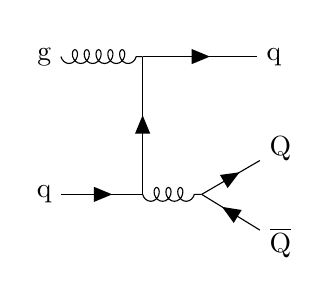
\begin{tikzpicture}
        \begin{feynman}
          \vertex (a) {g};
          \vertex[above=0.25cm of a] (spacing) {$ $  }; 
          \vertex[right=1.25cm of a] (b);
          \vertex[right=1.45cm of b] (c) {q};
          \vertex[below=1.75cm of a] (d) {q};
          \vertex[right=1.25cm of d] (e);
          \vertex[right=0.75cm of e] (f);
          \vertex[right=1cm of f] (g);
          \vertex[above=0.3cm of g] (h) {Q};
          \vertex[below=0.3cm of g] (j) {$\overline{\mathrm{Q}}$};
          \diagram* {
                (a) -- [gluon] (b),
                (d) -- [fermion] (e) -- [fermion] (b) -- [fermion] (c),
                (e) -- [gluon] (f),
                (j) -- [fermion] (f) -- [fermion] (h),
          };
        \end{feynman}
      \end{tikzpicture}\quad
    \caption{Feynman diagrams contributing to the first order corrections of the heavy-flavour production cross-section calculations.}
    \label{fig:NLO_diagrams}
\end{figure}

\begin{sloppypar}
Because of their large masses, heavy quarks can only be produced through hard-scattering processes, characterised by momentum transfers of the order of \mbox{$Q^2 \geq 4m^2_\mathrm{b,c}$}. In this regime, the strong coupling constant is significantly smaller than unity, allowing for the perturbative calculation of the heavy quark production cross-section from partonic scattering using QCD. While predictions at next-to-next-to-next-to-leading order (N$^3$LO) are available for certain processes, such as Higgs production~\cite{Anastasiou:2015vya, Anastasiou:2016cez}, the current state-of-the-art calculations for charm-quark production are at next-to-leading order (NLO) with all-order resummation to next-to-leading logarithmic (NLL) accuracy in the limit where the \pt of a heavy quark is much larger than its mass~\cite{Cacciari:1998it}. The contributions arising at the NLO include 1-loop virtual corrections to the Born process and real emission of a gluon or a quark-antiquark pair, and are depicted in Fig~\ref{fig:NLO_diagrams}. Next-to-next-to-leading order (NNLO) QCD radiative corrections to the production of bottom-quark pairs have also been computed~\cite{Catani:2020kkl}.
\end{sloppypar}

\subsection{Fragmentation Functions}
\begin{sloppypar}
Quarks and gluons produced in hard-scattering processes ultimately give rise to colourless observable hadrons. The associated process, known as hadronisation, is non-perturbative since the partonic processes involved are characterised by relatively small energy scales ($\sim\Lambda_\mathrm{QCD}$), where the strong coupling constant is large. The hadronisation process is described by the Fragmentation Functions (FFs) $D_\mathrm{Q\rightarrow H_Q}(z,\mu_\mathrm{F}^2)$, which parametrise the probability of the heavy quark Q to fragment into a heavy-flavour hadron $\mathrm{H_Q}$ with a fraction of the parent parton momentum $z$. They provide a simple ``effective" description of the parton-to-hadron transition by mapping the quark-momentum-differential cross-section into the hadron-momentum differential one. FFs are typically determined from experimental data, usually by analyzing the final-state hadrons produced in electron-positron collisions where the initial momenta are well-known. These FFs are then applied in the evaluation of cross-sections in other colliding systems, assuming that the relevant hadronisation processes are “universal”, i.e., independent of the collision energy and system. This assumption implies the hypothesis of \emph{independent fragmentation}, which states that the hadronisation of the parton produced in the hard-scattering process is independent of the production mechanism and the partonic environment which surrounds it. Differently from the fragmentation of light quarks and gluons, kinematic considerations on heavy-quark fragmentation~\cite{Bjorken:1977md,Suzuki:1977km} suggest that heavy hadrons tend to carry a larger fraction of the parent parton momentum. Fragmentation functions for heavy quarks are therefore shifted towards higher values of $z$ compared to those of light quarks and gluons~\cite{Peterson:1982ak}. Many FFs have been determined from global fits to data, such as the NNFF1.1h~\cite{Bertone:2018ecm}, DSS~\cite{deFlorian:2007aj}, and KKP~\cite{Kniehl:2000fe} parametrisations for light flavours, and typically differ in the data sets used for the fit, the treatment of the data, and the functional form of the FFs. Parametrisations for heavy quark fragmentation include that of Peterson et al.~\cite{Peterson:1982ak}, Kartvelishvili et al.~\cite{Kartvelishvili:1977pi}, and Breetan et al.~\cite{Braaten:1994bz}. Similarly to PDFs, FFs also evolve with the energy scale of the interaction, and this evolution is described perturbatively by the DGLAP equations. 
\end{sloppypar}

\section{Hadronisation: microscopic and macroscopic descriptions}\label{sec:hadronisation}
Despite being a very powerful effective tool for describing heavy-flavour hadron production, the parametrisation of fragmentation functions used in a factorisation-theorem approach is not the only method used to describe the hadronisation of energetic quarks in high-energy collisions. Over the years, other models have been developed to describe hadron production starting from a partonic stage (e.g., quarks and gluons from the initial hard-scattering process, and those being radiated from the initial partons) and implementing a colour neutralisation procedure that groups quarks and gluons into hadrons.

The standard approach for describing the complex event topologies in these models, which are typically implemented in Monte Carlo event generators, begins with a matrix-element calculation for the production of a few well-separated partons, followed by the application of a parton shower. The \emph{parton shower} provides an approximate perturbative treatment of QCD dynamics, which is then combined with a non-perturbative model for the hadronisation process at a certain infrared cut-off scale, typically taken to be of the order of 1~\gev. The basic idea of the parton shower relies on the Sudakov form factor~\cite{Sudakov:1954sw}, which expresses the probability of a parton not radiating another parton in a given phase space region. If a parton does radiate, the newly-produced parton becomes the source of a new cascade, continuing until the parton shower terminates at the hadronisation scale. At this point, partons are allowed to fragment into hadrons through hadronisation models. 

Although several hadronisation models have been developed, each implementing a different approach to the description of this non-perturbative process, a common feature is the hypothesis of local parton-hadron duality~\cite{Azimov:1984np}, which states that the flow of momentum and quantum numbers at the hadron level tends to follow the flow established at the parton level.

\subsection{Independent fragmentation}\label{sec:independent_fragmentation}
The description of the hadronisation process using FFs relies on the assumption of \emph{independent fragmentation}, i.e., the probability of a parton fragmenting into a hadron is considered independent of the other partons produced in the same collision, effectively considering the hadronisation process as universal, i.e., independent of the collision energy and system. In the original scheme proposed by R. Field and R. Feynman~\cite{Field:1976ve}, the fragmenting quark combines with an antiquark from a $\mathrm{q\overline{q}}$ pair produced from the vacuum to create a meson with energy fraction $z$. The remaining quark, with energy fraction $(1-z)$, fragments in the same way, continuing until an energy cut-off is reached. The probability distribution of $z$ is the fragmentation function. The assumption of independent fragmentation is valid in the case of low-multiplicity \ee collision events, where the number of produced partons is small and no hadronic remnants are present.

However, recent results on the production of strange and heavy-flavour baryons in proton-proton and proton-lead collisions at the LHC~\cite{ALICE:2020wla,ALICE:2024ozd} show that a description of the hadronisation process based on independent fragmentation is not sufficient to describe the data, as it significantly underestimates the baryon production. Figure~\ref{fig:Lambda_c_D0_ee} shows the $\mathrm{\lc/D^0}$ production-yield ratio measured at midrapidity ($\lvert y\rvert<0.5$) in pp collisions at $\sqrt{s} = 5.02$~\tev by the ALICE Collaboration~\cite{ALICE:2020wla} as a function of \pt, compared to theoretical predictions. The predictions are obtained from: i) \textsc{Pythia}~8 with Monash tune~\cite{Skands:2014pea}; ii) HERWIG~7~\cite{Bellm:2015jjp}; iii) POWHEG~\cite{Frixione:2007nw} NLO pQCD calculations, matched with \textsc{Pythia}~6 to generate the parton shower; iv) General-Mass Variable-Flavour-Number Scheme~\cite{Kniehl:2005mk} (GM-VFNS) NLO pQCD calculation with next-to-leading-log resummation. All these models, whose details are described in the following sections, implement fragmentation processes tuned on results of charm production measurements is \ee collisions, and predict an almost \pt-independent $\mathrm{\lc/D^0}$ ratio of around 0.1, significantly underestimating the values measured in pp collisions by a factor of about 5 at low \pt.

\begin{figure}[htb]
  \centering
  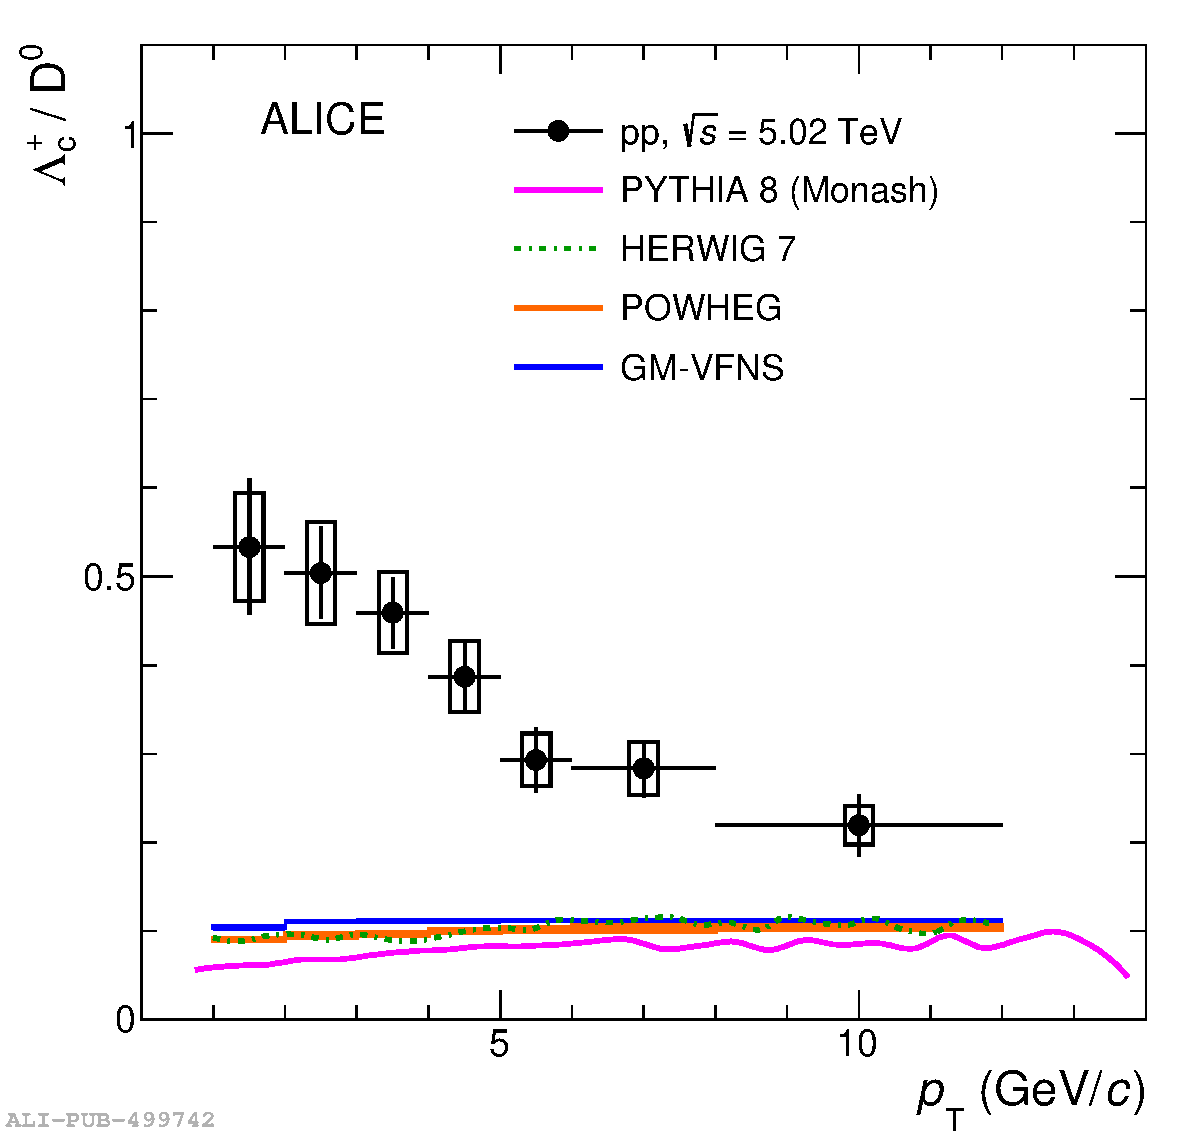
\includegraphics[width=0.7\linewidth]{Figures/Chapter 2/LcD_models_withFFModels_ropes_2.pdf}
  \caption{$\mathrm{\lc/D^0}$ production-yield ratio measured at $\sqrt{s} = 5.02$~\tev by the ALICE Collaboration as a function of \pt, compared to theoretical predictions. Figure taken from Ref.~\cite{ALICE:2020wla}.}
  \label{fig:Lambda_c_D0_ee}
\end{figure}


\subsection{String model}
\begin{figure}[htb]
    \centering
    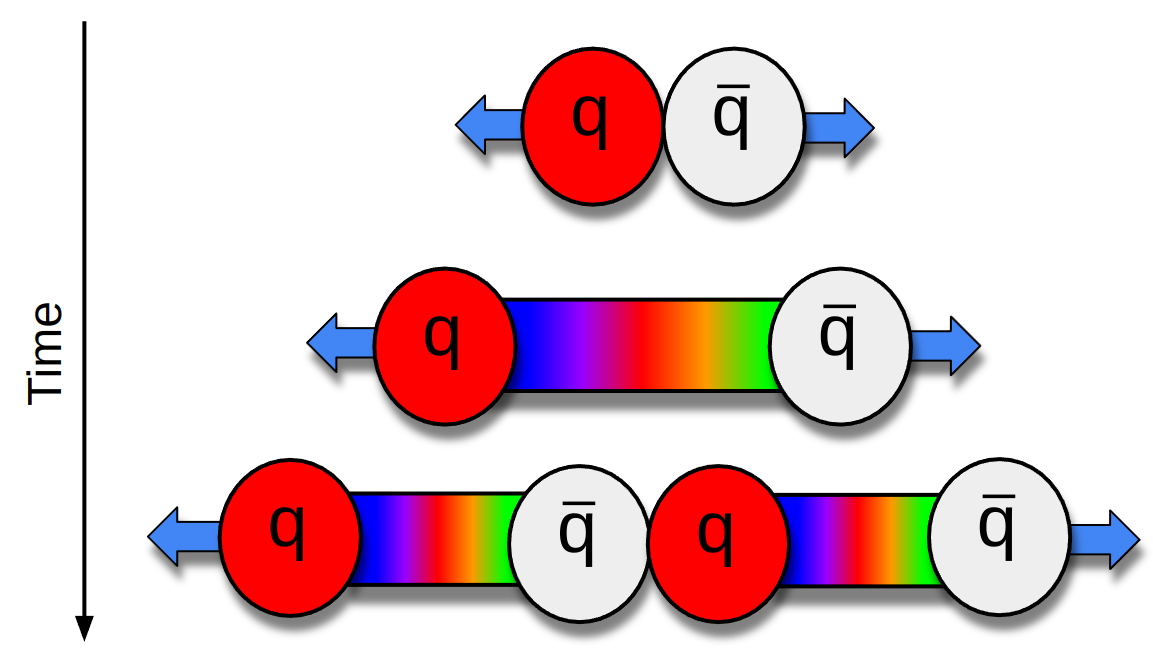
\includegraphics[width=0.7\linewidth]{Figures/Chapter 2/Lund.png}
    \caption{Schematic representation of the Lund string model hadronisation process.}
    \label{fig:Lund}
\end{figure}
The most widely used model for the description of the hadronisation process in Monte Carlo event generators is the Lund string model~\cite{Andersson:1983ia}, employed in the \textsc{Pythia} event generator~\cite{Bierlich:2022pfr}. In this model, the strong force between quarks and gluons is modelled in terms of a colour string with energy given by the Cornell potential~\cite{Eichten:1974af},
\begin{equation*}
    V(r) = -\frac{A(r)}{r} + \kappa r\quad .
\end{equation*}
Since the linear term is dominant, the Cornell potential is typically approximated as $V(r) = \kappa r$, with $\kappa\sim1$~\gev/fm. This implies that a constant force is exerted between the quarks, leading to a linear increase in the potential energy with increasing distance between the quarks. When back-to-back quarks are produced in a hard-scattering process, they move apart, causing the string to stretch and accumulate energy. When the energy stored in the string becomes large enough, it becomes energetically convenient to materialise a quark-antiquark pair with mass $m_\mathrm{q}$ from the colour flux tube, making the string break. The probability of string breaking is given by~\cite{Andersson:1983jt}
\begin{equation}\label{eq:P_string_breaking}
    P \propto \mathrm{exp}\left(-\frac{\pi m_\mathrm{T,q}^2}{\kappa}\right) = \mathrm{exp}\left(-\frac{\pi m_\mathrm{q}^2}{\kappa}\right) \mathrm{exp}\left(-\frac{\pi p_\mathrm{T,q}^2}{\kappa}\right)\quad .
\end{equation}
This string-braking process continues until the energy of the string is below the threshold for producing new quark-antiquark pairs, effectively modelling the parton fragmentation mechanism and applying the infrared cut-off introduced in Sec.~\ref{sec:hadronisation}.

The mass dependence of Eq.~\ref{eq:P_string_breaking} leads to a Gaussian suppression factor that limits the probability for the colour field to produce quark-antiquark pairs for heavier flavours. The $\mathrm{s\overline{s}}$ and $\mathrm{c\overline{c}}$ pair production probability can be estimated with respect to that for $\mathrm{u\overline{u}}$ and $\mathrm{d\overline{d}}$ pairs~\cite{Ferreres-Sole:2018vgo}, yielding
\begin{equation*}
    \mathrm{u : d : s : c} \sim 1 : 1 : 1/3 : 10^{-11}\quad .
\end{equation*}
The production of $\mathrm{c\overline{c}}$ pairs in string-breaking (non-perturbative) processes results significantly suppressed, by a factor of $10^{-11}$, compared to $\mathrm{u\overline{u}}$ pairs. Such quarks are therefore almost exclusively produced in hard-scattering processes, quantitatively confirming the qualitative discussion in Sec.~\ref{sec:partonic_cross_section} on the feasibility of using perturbative QCD to describe the production of heavy-flavour quarks.

The fragmentation model described above shares many similarities with the independent fragmentation model discussed in Sec.~\ref{sec:independent_fragmentation}, with the main difference being the pictorial description of interactions with a colour string connecting the quarks. However, the gluon radiation has been neglected until now. A significant difference emerges once the gluon bremstrahlung is considered~\cite{Sjostrand:1984ic}. 

In this framework, gluons are represented as carrying both a colour and an anticolour charge. Therefore, in a three-parton system ($\mathrm{qg\overline{q}}$), the quark is colour-connected to the anticolour index of the gluon, and the colour index of the gluon is connected to the antiquark. The interaction between the quark-antiquark pair is suppressed by a factor 1/$\mathrm{N_c}$, where $\mathrm{N_c}$ is the number of colours, and can be neglected in a leading-colour approximation ($\mathrm{N_c} \rightarrow\infty$). The presence of the gluon produces a corner, or “kink”, on the string. The Lorentz boost of a string causes the hadrons formed through its breaking to go preferentially in the direction of its motion. Most hadrons that the q-g string segment produces will go between the quark and the gluon, while hadrons from the $\mathrm{\overline{q}\text{-}g}$ string will go between the gluon and the antiquark. Only very few hadrons will go between the quark and the antiquark. This behaviour leads to an angular distribution of hadrons in \ee three-jet final states which differs from that predicted by independent fragmentation and is found to be in better agreement with experimental results. 

\subsubsection{Non-independent fragmentation and multiple parton interactions}
To fully describe hadron production in high-energy collisions, the description of the fragmentation process through colour-string breaking in a parton shower, coupled with a hadronisation step, is not sufficient. A definition of the ways in which the partons produced in the hard-scattering process can be connected to hadronise is also needed. At leading-colour approximation, in the partonic final states, each quark is colour-connected to a single other parton in the event. Since gluons carry both a colour and an anticolour charge, they are connected to two other partons. With this approximation, the Lund model provides a good description of measurements in \ee collisions, where a parton-rich environment is not produced. However, recent results on the production of strange and heavy-flavour baryons in proton-proton and proton-lead collisions at the LHC~\cite{ALICE:2022exq,ALICE:2024ozd} show that a description of the hadronisation process based on independent fragmentation is not sufficient to describe the data, as it significantly underestimates the charm-baryon production.

In hadronic collisions, one must consider that to achieve a comprehensive description of a given process, a description of coloured initial-state partons and the associated beam remnants should be taken into account, as they hadronise and may potentially interact with each other. Furthermore, new insights on the underlying event and soft-physics processes occurring in a hadronic collision suggest that such events are dominated by Multiple Parton Interactions (MPI), where two or more distinct hard parton interactions occur in a single hadron-hadron collision. MPI produce densely-populated partonic environments in which colour string can be formed between partons from different hard-scattering processes. Phase-space overlaps among the partons produced in the MPIs become more likely as the number of MPI increases, and are expected to play a more important role in pp collisions with higher particle multiplicities. Their non-independent hadronisation should be considered for a more complete description of the process. 

New models based on colour-reconnection beyond the leading-colour approximation~\cite{Christiansen:2015yqa} have been developed, where the leading-colour connections produced in the partonic showers are rearranged to form new subleading topologies that would have been present in a full-colour treatment. New string configurations emerge in the beyond-leading-colour picture, as junction topologies and gluon loops are formed in addition to the standard $\mathrm{q\overline{q}}$ and q-g strings. In particular, junctions allow for an enhanced production of baryons, to account for the observed enhancement in the production of baryons in proton-proton and proton-lead collisions. Different configurations for the colour reconnections (\emph{CR modes}) are implemented in the \textsc{Pythia} event generator, applying different constraints on the possible colour reconnections.

\subsection{Cluster model}
A different approach to the description of the hadronisation process is the cluster model~\cite{Webber:1983if}, which is implemented in the HERWIG event generator~\cite{Bahr:2008pv}. It is based on the \emph{preconfinement} of colour~\cite{Amati:1979fg}, which arises from the observation that by following the colour structure of the parton shower and studying the colour-singlet pairs of colour-connected quark-antiquark states, one finds that they tend to end up close in phase space. This suggests that quarks and gluons produced in this evolution become organised in clusters of colour singlets with finite masses, i.e., the mass distribution of these clusters is independent of the hard scattering process and its centre-of-mass energy. The confinement can then convert these singlets of small mass into hadrons. 

The first step of the cluster hadronisation model is to non-perturbatively split the gluons left at the end of the parton shower into quark-antiquark pairs. Each gluon is allowed to decay into any of the accessible quark flavours with a probability given by the available phase space for the decay. 

Then, the hadronisation process takes place. The key idea is based on the ansatz that the cluster mass spectrum is both universal and steeply falling at high masses. Therefore, the clusters can be regarded as highly excited hadron resonances and decayed, according to phase space, into the observed hadrons. Before the actual cluster decays, a few heavier clusters are split into lighter clusters (\emph{cluster fission}), for a more reasonable agreement with experimental results. A cluster is split into two clusters if its mass, $M$, is such that
\begin{equation*}
    M^{\mathrm{Cl_{pow}}} \geq \mathrm{Cl_{max} {}^{Cl_{pow}}} + (m_1+m_2)^{\mathrm{Cl_{pow}}}\quad ,
\end{equation*}
where $\mathrm{Cl_{max}}$ and $\mathrm{Cl_{pow}}$ are parameters of the model, and $m_{1,2}$ are the masses of the constituent partons of the cluster. For clusters that need to be split, a $\mathrm{q\overline{q}}$ pair is produced from the vacuum. Only up, down, and strange quarks are chosen with probabilities given by other model parameters. Once a $\mathrm{q\overline{q}}$ pair is produced, the cluster is split into two new clusters with one of the original partons in each cluster. 

Finally, the cluster is decayed into a pair of hadrons. For a cluster of a given flavour ($\mathrm{q_1, \overline{q}_2}$), a quark-antiquark or diquark-antidiquark pair is extracted from the vacuum and a pair of hadrons with flavours $\mathrm{q_1}$ and $\mathrm{q_2}$ is formed. The hadrons are selected from all the possible hadrons with the appropriate flavour based on the available phase space, spin and flavour. As a consequence, heavier hadrons are suppressed, leading to a natural description of the baryon and strangeness suppression. The cluster model was found to describe data reasonably well, with far fewer parameters than the string model~\cite{Seymour:2013ega}.

\subsection{Coalescence model}
\begin{figure}[htb]
    \centering
    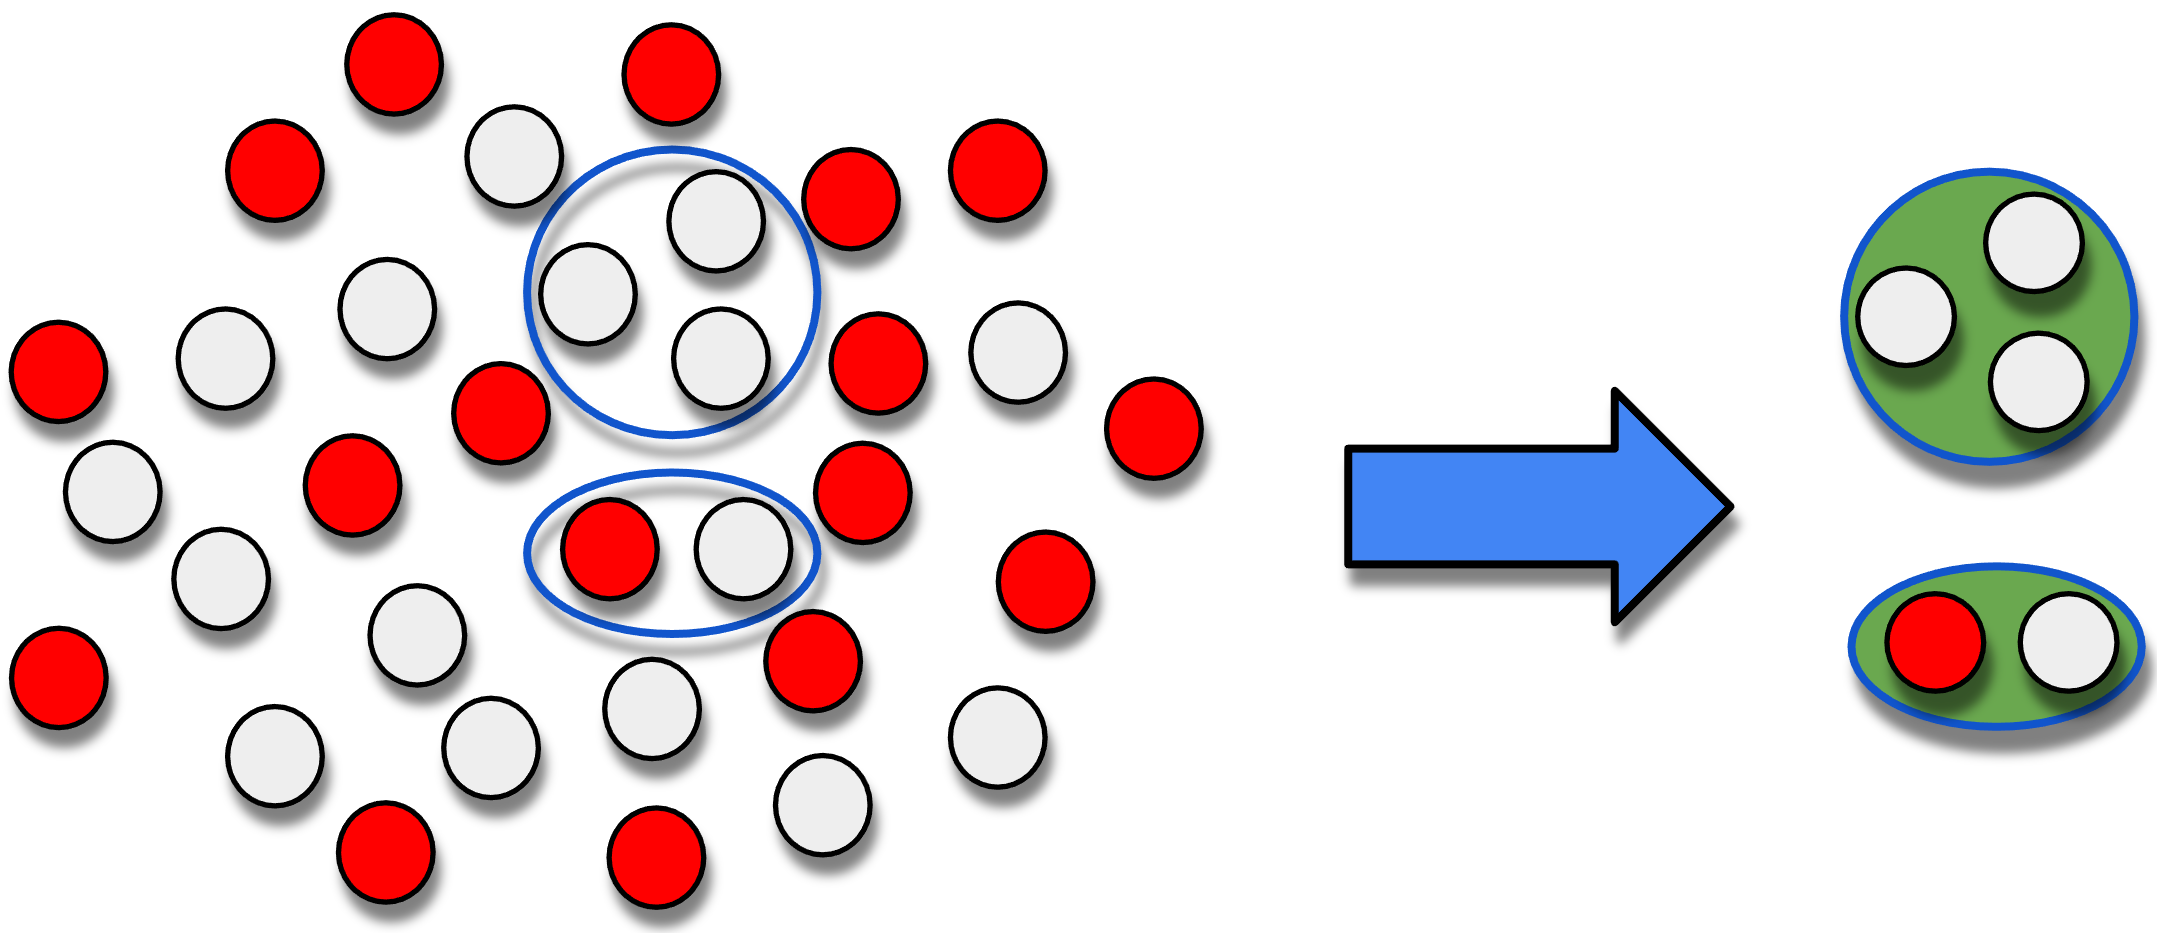
\includegraphics[width=0.7\linewidth]{Figures/Chapter 2/Coalescence.png}
    \caption{Representation of hadron production via recombination.}
\end{figure}

As outlined in Sec.~\ref{sec:high_pt}, the hadronisation process can be modified in the presence of a strongly-interacting deconfined medium. A novel mechanism for the production of hadrons, the recombination (also called coalescence), can take place in a thermalised system such as the QGP. When recombination occurs, two or three quarks close in the space-velocity phase space can bind together to form a hadron, which will have a higher (transverse-) momentum than the quarks that combined to form the hadron. This is different from the case of fragmentation, in which an energetic parton produces hadrons with lower momentum than the parent quark. As a consequence, the \pt distribution of hadrons formed by coalescence differs from the one expected from fragmentation. In particular, the hadron \pt is shifted to larger values as compared to fragmentation. Due to the steeply-falling quark \pt spectrum, this leads to a depletion of the low-\pt hadron yield, and an enhancement of the intermediate-\pt hadron yield. In addition, due to the relatively high abundance of low-\pt quarks and the sparsity of high-\pt partons, an enhancement of baryon-to-meson production-yield ratios at intermediate \pt is expected in proton-proton collisions when compared to \ee collisions as a natural consequence of the recombination mechanism. 

Models implementing the coalescence mechanism can effectively describe the production of hadrons in heavy-ion collisions. Intriguingly, models implementing recombination that successfully describe the production and azimuthal anisotropy of charm hadrons in these collisions, fail in doing so when this process is de-activated, as shown in Fig.~\ref{fig:D_recombination} for the case of prompt D mesons in the heavy-flavour sector. The D-meson \raa measured in the 0--10\% centrality interval and the second coefficient $v_2$ of the Fourier transform of the azimuthal distribution of D mesons in the 30--50\% centrality range measured by the ALICE Collaboration at midrapidity ($\lvert y\lvert<0.5$ for the \raa measurement and $\lvert y\lvert<0.8$ for that of the $v_2$ coefficients) at $\snn=5.02$~\tev~\cite{ALICE:2021rxa} are illustrated in the left and right panels, respectively. The measurements are compared to the Parton-Hadron-String Dynamics~\cite{Cassing:2008sv} (PHSD), POWLANG~\cite{Beraudo:2014boa}, and DAB-MOD~\cite{Katz:2019fkc} predictions, which are provided with (solid line) and without (dashed line) the implementation of the recombination process in the hadronisation mechanism. The calculations performed including the recombination of charm quarks with light quarks provide a good description of the experimental results, while they fail to reproduce the data when recombination is turned off. This suggests that the recombination mechanism plays a relevant role in the description of heavy-flavour hadron production in heavy-ion collisions.
\begin{figure}[htb]
  \centering
  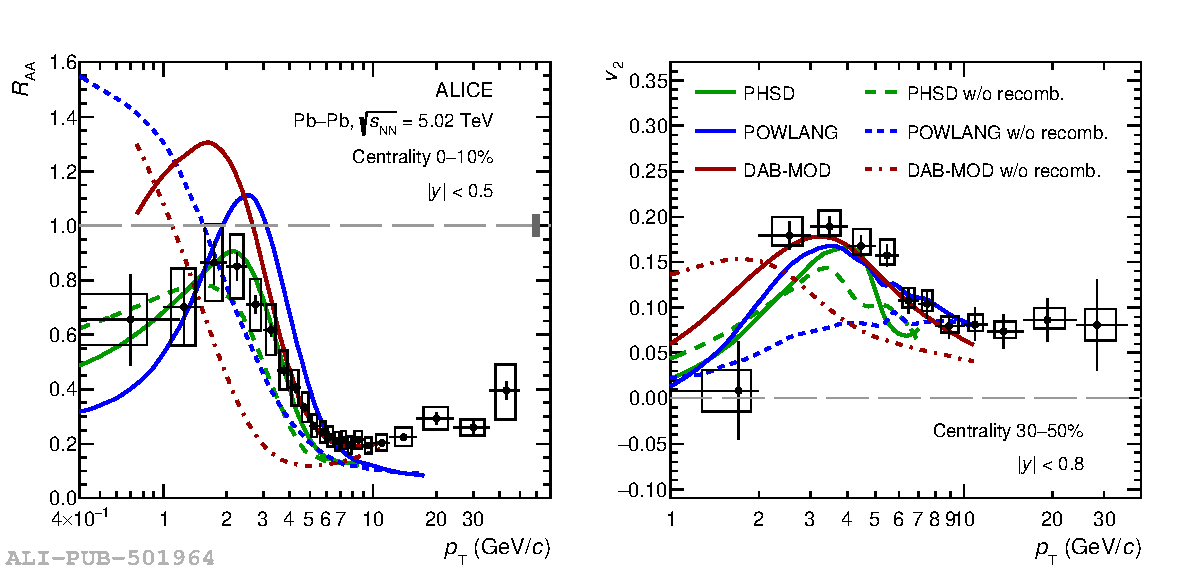
\includegraphics[width=\linewidth]{Figures/Chapter 2/D_Raa010_V23050_FragCoal_3models_1.pdf}
  \caption{Prompt D-meson $R_\mathrm{AA}$ in the 0--10\% centrality class (left panel) and $v_2$ in the 30--50\% centrality class (right panel) compared with predictions obtained with and without including hadronisation via recombination. Figure taken from Ref.~\cite{ALICE:2021rxa}.}
  \label{fig:D_recombination}
\end{figure}

New experimental measurements in pp and p--Pb collisions at the LHC~\cite{ALICE:2024ozd,ALICE:2016fzo,ALICE:2020wla,ALICE:2020wfu,ALICE:2021bli,CMS:2015fgy} provided a wealth of results suggesting that certain phenomena that are observed in nuclear collisions, such as strangeness enhancement and flow, may also occur in smaller collision systems. These effects are typically related to the presence of an expanding medium, thus raising the question of whether the coalescence hadronisation mechanism could also play a role in small collision systems. A hint that this could be the case comes from the observation that the production of charm baryons in pp and p--Pb collisions~\cite{ALICE:2022exq,ALICE:2024ozd} is significantly larger than expected from models based on a fragmentation tuned on \ee collisions. 

Various models have been developed in order to describe the observed charm-baryon enhancement in proton-proton and proton-lead collisions with the assumption of a recombination mechanism. These include the Quark (re-)Combination Mechanism~\cite{Song:2018tpv} (QCM) model, where coalescence between a charm quark and equal-velocity light quarks takes place at all momenta, and thermal weights are applied to account for relative production of scalar and vector mesons. In this model, the quark spectra are parametrised based on measurements of light-flavour hadrons and D-mesons. Other models adopt a description of the expanding system using a hydrodynamic approach and implementing hadronisation of the medium via a combination of coalescence and independent fragmentation. The Catania coalescence model~\cite{Minissale:2020bif} describes a thermalised system of u, d, s quarks, and gluons, where the charm quark can hadronise via either fragmentation or coalescence with light quarks from the bulk. The POWLANG model~\cite{Beraudo:2023nlq} predicts the formation of a small, deconfined, and expanding fireball in proton-proton collisions, where charm quarks are subject to rescattering and hadronisation, and can recombine with light quarks as in heavy-ion collisions. 

Each of these models provides a different hadronisation mechanism in proton-proton collisions compared to \ee ones, and independent hadronisation is no longer assumed. They improve the description of the data, achieving a better agreement with experimental results such as the \pt dependence of $\Lambda_\mathrm{c}^+/\mathrm{D}^0$ and $\Xi_\mathrm{c}^0/\mathrm{D}^0$ baryon-to-meson production-yield ratios.

\subsection{Core-corona model}
Core-corona models~\cite{Werner:2007bf} offer an intermediate approach between the two presented above. In these models, the fireball is divided into a high-density core part, treated with hydrodynamics and thermal modelling of particle production, similarly to that implemented in the SHM introduced in Sec.~\ref{subsec:SHM}, and a corona part, described using the Lund string model. This framework is based on the assumption that small QGP droplets may only be produced once the density is high enough. The EPOS Monte Carlo event generator~\cite{Porteboeuf:2008fgf} implements such a picture, and provides a very competitive description of data.

\subsection{Statistical hadronisation model}
The last model presented in this section exploits the idea of a thermalised system, which is by definition in thermal equilibrium. A macroscopic approach to hadronisation, based on a statistical model, can be used to describe the charm-hadron production in hadronic collisions. The principles of thermodynamics can be applied to the hadronisation process, where the hadron yields are determined by the hadron's mass and the temperature and baryon chemical potential of the system. As described in Sec.~\ref{subsec:SHM}, this approach has been successfully adopted to describe the light and strange hadron production in heavy-ion collisions and smaller systems. 

Different approaches are used to predict the production of light- and heavy-flavour hadrons with the SHM. Due to the large masses of charm and beauty quarks, which are significantly larger than the temperature of the QGP, their thermal production in the medium is strongly suppressed. Therefore, the production of charm and beauty quarks is determined by their initial production in the hard-scattering processes. Their distribution into hadrons is then predicted with thermal weights. A charm balance equation is used to ensure the conservation of the initially produced charm quarks into the final-state hadrons via a fugacity factor $g_\mathrm{c}$, which accounts for the absence of chemical equilibrium for heavy quarks. In addition, the description of heavy-flavour hadron production and the baryon enhancement in this framework requires the inclusion of a strong feed-down from an augmented set of excited charm- or beauty-baryon states, not included in the PDG~\cite{pdg}. Recent model developments~\cite{He:2019tik,He:2022tod} have extended the Statistical Hadronisation Model (SHM) to include a set of 18 $\mathrm{\Lambda_c}$'s, 42 $\mathrm{\Sigma_c}$'s, 62 $\mathrm{\Xi_c}$'s, and 34 $\mathrm{\Omega_c}$'s excited states up to a mass of 3.5~\gev, predicted by the Relativistic Quark Model~\cite{Ebert:2011kk}. Such models provide a good description of the measured $\mathrm{\lc/D^0}$ production yield ratio and the \pt spectra of D mesons and \lc at midrapidity.

\subsection{Baryon enhancement: \texorpdfstring{$\mathrm{\lc/D^0}$}{Lc/D0} ratio}
\begin{figure}[htb]
    \centering
    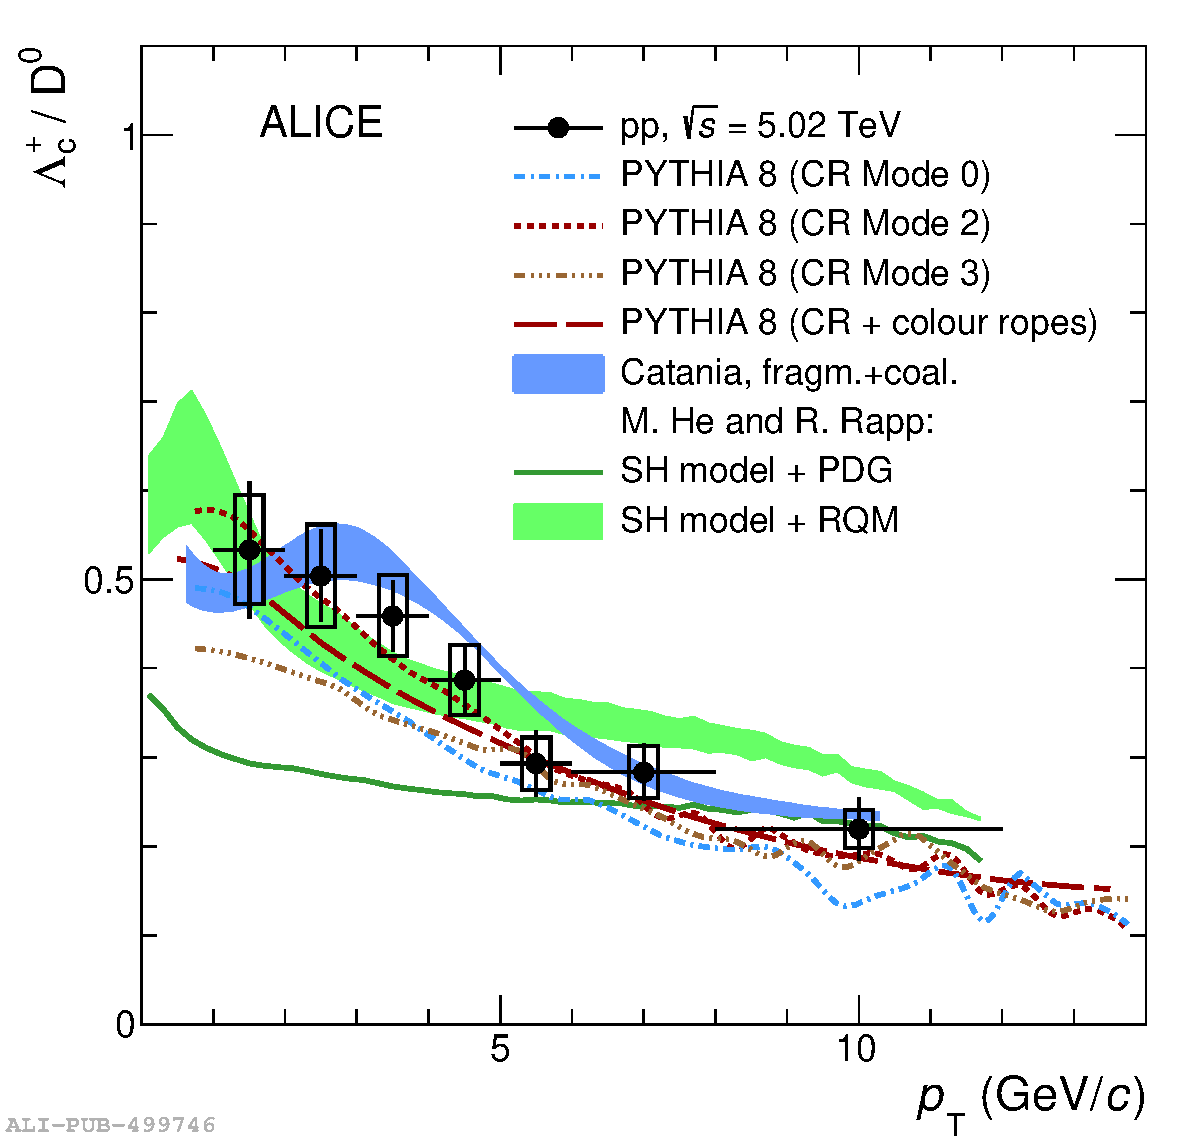
\includegraphics[width=0.48\linewidth]{Figures/Chapter 2/LcD_models_withModifiedModels_ropes_coal_2.pdf}
    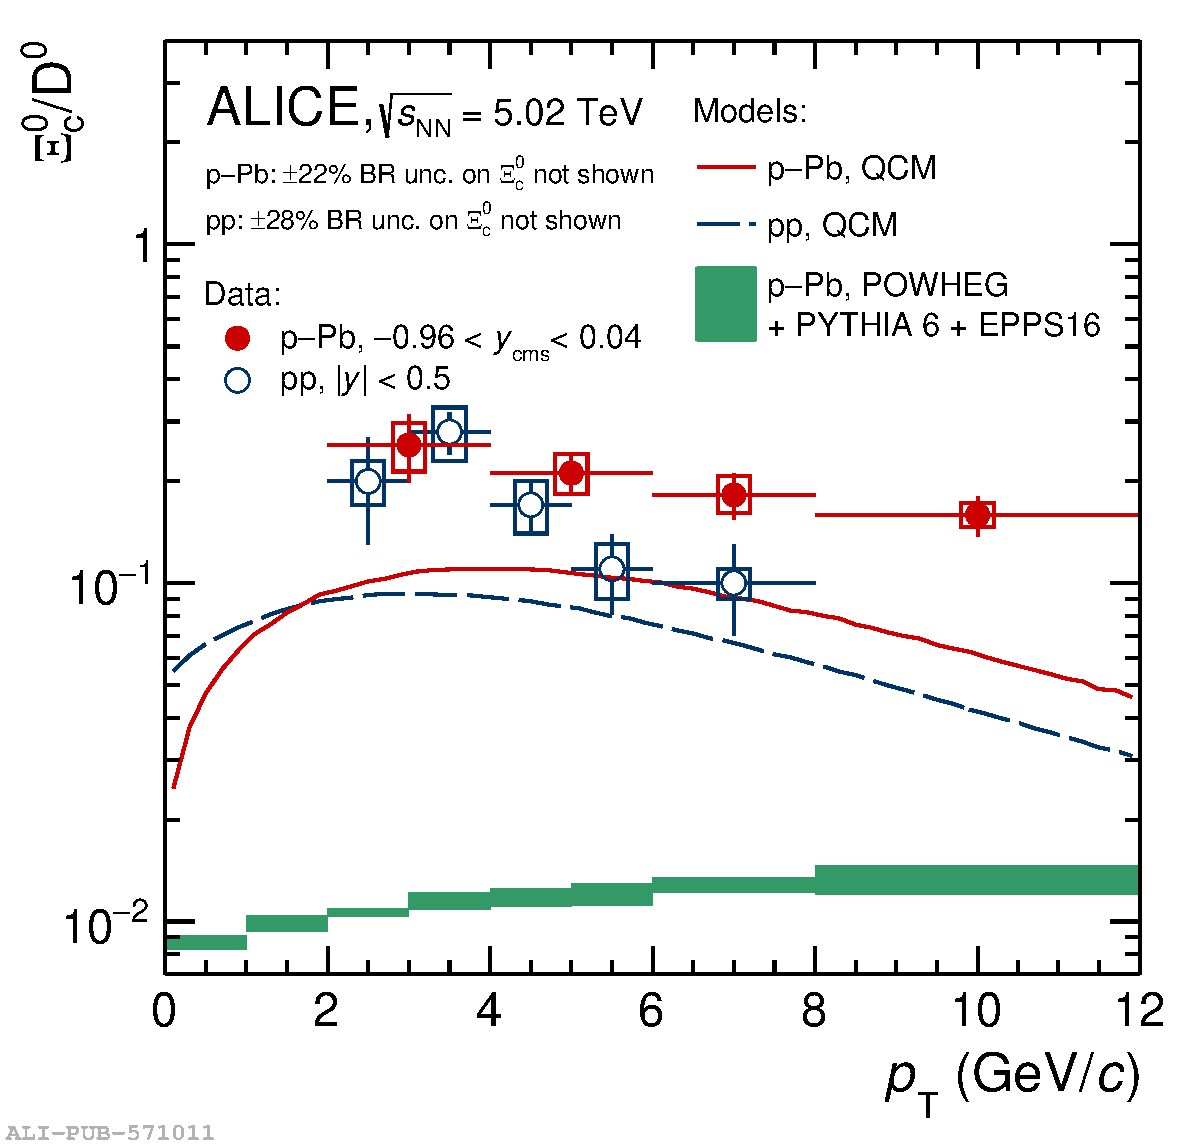
\includegraphics[width=0.48\linewidth]{Figures/Chapter 2/Xic0_D0_Ratio.pdf}
    \caption{Left panel: $\mathrm{\lc/D^0}$ production-yield ratio measured at midrapidity ($\lvert y\rvert < 0.5$) in pp collisions at $\sqrt{s} = 5.02$~\tev by the ALICE Collaboration~\cite{ALICE:2020wla} as a function of \pt, compared to theoretical predictions. Right panel: $\mathrm{\Xi_c^0/D^0}$ production-yield ratio measured at midrapidity ($-0.96 < y < 0.05$) in p--Pb collisions at $\snn = 5.02$~\tev by the ALICE Collaboration~\cite{ALICE:2020wla} as a function of \pt, compared to theoretical predictions. Figures taken from Refs.~\cite{ALICE:2020wla} and~\cite{ALICE:2024ozd}.}
    \label{fig:Lambda_c_D0}
\end{figure}
The hadronisation process can be experimentally studied through the measurement of production-yield ratios of hadrons. Since the initial state of the collision and the charm production cross-section is the same for all charm hadrons, the measurement of the production-yield ratio of different charm hadrons can be expressed, using the factorisation theorem, as the ratio of the fragmentation functions of the hadrons, which describe the hadronisation process. 

The left panel of Fig.~\ref{fig:Lambda_c_D0} shows the $\mathrm{\lc/D^0}$ baryon-to-meson production-yield ratio measured at midrapidity ($\lvert y\rvert < 0.5$) in pp collisions at $\sqs = 5.02$~\tev by the ALICE Collaboration as a function of \pt, compared to models that include mechanisms to enhance baryon production compared to those in which the hadronisation is implemented through independent fragmentation and parametrised on results from \ee collisions, already presented in Fig.~\ref{fig:Lambda_c_D0_ee}. They include i) \textsc{Pythia}~8 simulations with colour-reconnection beyond the leading-colour approximation~\cite{Christiansen:2015yqa} (three colour reconnection modes (0,2,3), which apply different constraints on the allowed reconnection are considered); ii) \textsc{Pythia}~8 with colour-reconnection plus rope hadronisation~\cite{Bierlich:2014xba} where colour charges can act coherently to form a rope, increasing the effective string tension; iii) Catania coalescence model~\cite{Minissale:2020bif}, where a QGP is formed in pp collisions and hadronisation occurs through both recombination and fragmentation; iv) SHM~\cite{Braun-Munzinger:2003pwq} where the underlying charm baryon spectrum is either taken from the PDG~\cite{pdg}, or augmented to include additional excited baryon states, which have not yet been observed but are predicted by the RQM~\cite{Ebert:2011kk}. These models are capable of describing both the magnitude and the \pt dependence of the $\mathrm{\lc/D^0}$ ratio, suggesting that the hadronisation process in proton-proton collisions might differ from that in \ee collisions. This conclusion is also confirmed by the measurement of the $\mathrm{\Xi_c^0/D^0}$ baryon-to-meson production-yield ratio at midrapidity ($-0.96<y<0.04$) in p--Pb collisions at $\snn = 5.02$~\tev performed by the ALICE Collaboration~\cite{ALICE:2024ozd}, shown in the right panel of Fig.~\ref{fig:Lambda_c_D0}. The measured ratio is compared to POWHEG~\cite{Frixione:2007nw} NLO pQCD calculations, matched with \textsc{Pythia}~6~\cite{Sjostrand:2006za} to generate the parton shower and fragmentation, which is tuned on \ee collisions, and to the EPPS16  parametrisation of the modification of the PDFs in the nuclear environment of the lead ion~\cite{Eskola:2016oht}. It predicts a slightly increasing trend with \pt, and undershoots the measured $\mathrm{\Xi_c^0/D^0}$ by a large factor of around 20. Predictions from the QCM model~\cite{Song:2018tpv} implementing a coalescence hadronisation mechanism provide a better description of both the \pt dependence and the magnitude of the data. 

The influence of the surrounding environment in the hadronisation of the charm quark could also potentially affect the relative abundances of strange and non-strange charm hadrons with increasing multiplicity from  \ee collisions to high multiplicity proton-proton and proton-nucleus collisions. Enhanced production of charm-strange hadrons may result from the coexistence of numerous strange quarks (which could be thermally produced in an environment with $T \gg m_\mathrm{s}$, as explained in Sec.~\ref{subsec:StrangenessEnhancement}) within the same region as the charm quark, thereby increasing the probability of recombination between them. This phenomenon can be studied through the measurement of the production-yield ratio of charm-strange hadrons to non-strange charm hadrons, such as the $\mathrm{D_s^+}$-meson to $\mathrm{D^+}$-meson ratio, which constitutes the primary focus of this Thesis.
\setcounter{chapter}{2}
%\chapter{A Large Ion Collider Experiment}

\lettrine[lines=6,findent=0.pt]{A}{LICE}  (A Large Ion Collider Experiment) is a general-purpose detector at the CERN LHC~\cite{ALICE:2008ngc}. It was conceived and built to focus on the study of QCD and heavy-ion collisions. It is designed to address the physics of strongly interacting matter and the quark-gluon plasma at extreme values of energy density and temperature in nucleus-nucleus collisions. Nonetheless, its physics programme also includes proton-proton and proton-nucleus collisions, which provide reference data for the heavy-ion programme and address a number of specific strong-interaction topics for which ALICE is complementary to the other LHC detectors. During the LHC Long Shutdown 2, between 2019 and 2021, ALICE underwent a major upgrade to improve its capabilities to probe the QGP with heavy-flavour quarks, and to enable completely new measurements of the thermal emission of dielectron pairs~\cite{ALICE:2023udb}.


\section{The Large Hadron Collider}
The Large Hadron Collider (LHC) is a two-ring superconducting hadron accelerator and collider based at CERN~\cite{Evans:2008zzb}, near Geneva in Switzerland. The LHC is the world's largest circular particle accelerator with a 26.7-kilometer circumference housed in a 3.8-meter-wide tunnel buried 50 to 175 meters underground, capable of accelerating protons up to energies of $\sqrt{s} = 14$~\tev and heavy ions $({}^{208}\mathrm{Pb}^{82+})$ up to $\sqrt{s_\mathrm{NN}}~=~5.5$~\tev. 
The LHC, which was used to host the Large Electron-Positron Collider (LEP), is the final stage of a chain of accelerators that provide protons and heavy ions with sufficient energy to be injected into the LHC, illustrated in Fig.~\ref{fig:LHC}. Protons are firstly collected by stripping electrons from a gaseous hydrogen source with an electric field and then grouped into bunches. The Linear accelerator 2 (Linac~2), the first linear accelerator in the LHC injection chain, accelerates the protons to 50~\mev. The protons are then injected into the Proton Synchrotron Booster (PSB), which accelerates them to 1.4~\gev, and then into the Proton Synchrotron (PS) and the Super Proton Synchrotron (SPS), reaching 25~\gev and 450~\gev, respectively. The protons are finally injected in the LHC, where they are accelerated up to a maximum energy of 7~\tev. In the LHC, the beams are forced to follow the circular path of the ring by strong magnetic fields $(\sim 8~\mathrm{T})$ produced by superconducting dipole magnets. Other magnets are used to steer and focus the beams in the interaction points. 

\begin{figure}[htb]
    \centering
    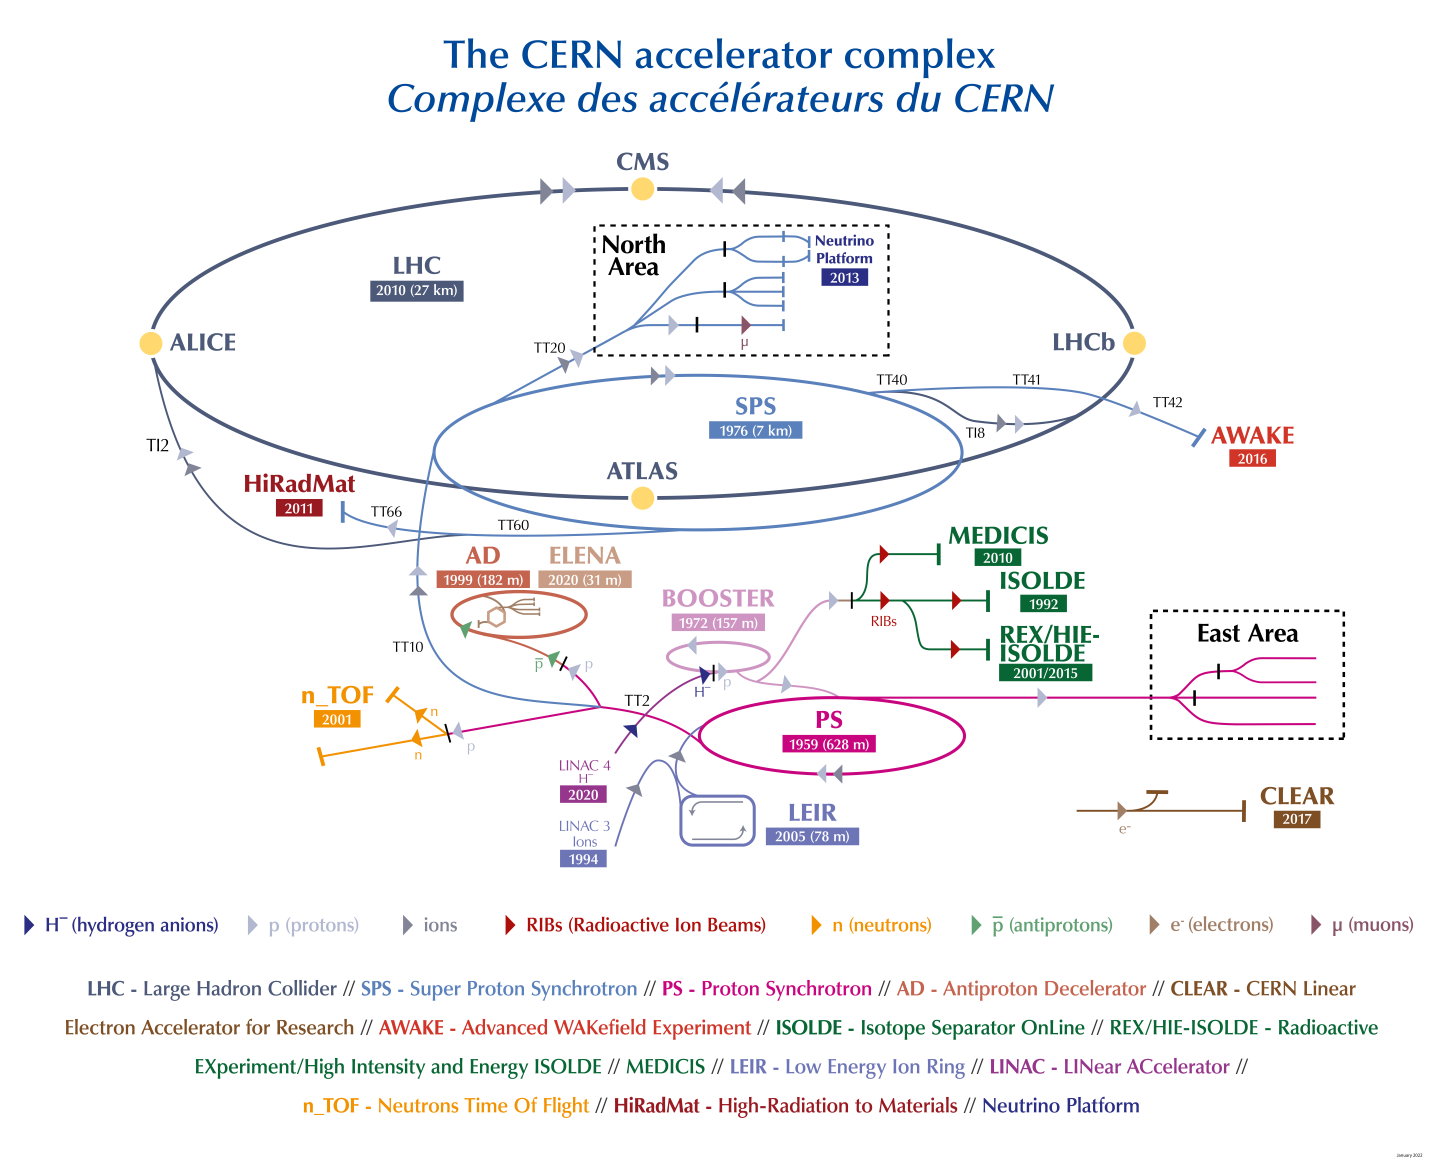
\includegraphics[width=\textwidth]{Figures/Chapter 3/LHC_Scheme.png}
    \caption{The Large Hadron Collider (LHC) accelerator complex at CERN.}
    \label{fig:LHC}
\end{figure}

Heavy-ion acceleration follows a similar path. The Pb ions (Pb$^{25+}$ -- Pb$^{28+}$) are extracted in the Electron-Cyclotron Resonance (ECR), and are focused in a Radio-Frequency Quadrupole (RFQ) using only electric fields. Pb$^{28+}$ ions with momentum of 2.5~\kevc are selected with a spectrometer, and are accelerated to 4.2~\mevc in the Linear accelerator 3 (Linac~3). A first \SI{0.5}{\micro\meter} copper stripping foil is then used to increase the charge state of the ions to Pb$^{53+}$. The PSB and PS accelerate the ions to 95.4~\mev A and 5.09~\gev. After the PS, a copper stripper ($\sim 1~\mathrm{mm}$) is used to further ionise the Pb ions to Pb$^{82+}$, which are then accelerated to 158~\gev in the SPS. The ions are finally injected into the LHC, where they are accelerated to 2.76~\tev per nucleon.

The LHC can collide protons with protons, protons with heavy ions, and heavy ions with heavy ions. The LHC has four main interaction points, where the four main detectors are located: A Large Ion Collider Experiment (ALICE), A Toroidal LHC ApparatuS (ATLAS), Compact Muon Solenoid (CMS), and LHC-beauty (LHCb). The four experiments were conceived and built to address different physics topics: ATLAS and CMS are general-purpose detectors designed to study the Higgs boson, which they discovered in 2012~\cite{ATLAS:2012yve,CMS:2012qbp} and to search for physics beyond the Standard Model; LHCb is dedicated to the measurement of beauty quarks as proxy for CP violation studies, and to the study of matter-antimatter asymmetry. ALICE is the only detector at the LHC that is dedicated to the study of QCD rather than the electroweak sector of the Standard Model. A more detailed description of the ALICE detector is given in the following sections.

\textcolor{red}{aggiungere luminosità istantanea}

\section{The ALICE experiment}
The physics programme of ALICE revolves around the study of the properties of strongly interacting matter at the extreme values of energy density and temperature reached in ultra-relativistic heavy-ion collisions. This unique environment poses several challenges, the most stringent one being the need to carry out measurements in a very high multiplicity environment. Originally, estimates for the charged particle multiplicity density at mid-rapidity in central Pb--Pb collisions ranged from $\de N/\de\eta = 2000$ up to almost $\de N/\de\eta = 8000$. Detectors with high granularity, fast readout capabilities, and highly radiation hardness were thus needed. The ALICE detector was designed to meet these requirements, and to provide a comprehensive set of measurements to study the properties of the QGP. The ALICE apparatus is shown in Fig.~\ref{fig:ALICE}. It is based on a central barrel, covering full azimuth ($0 < \varphi < 2\pi$) and the pseudorapidity region $\lvert \eta\rvert <0.9$ and a forward muon system with a dipole magnet providing a total bending power of 3~Tm, covering full azimuth and the pseudorapidity interval $-4.0 < \eta < -2.5$.

\begin{figure}
    \centering
    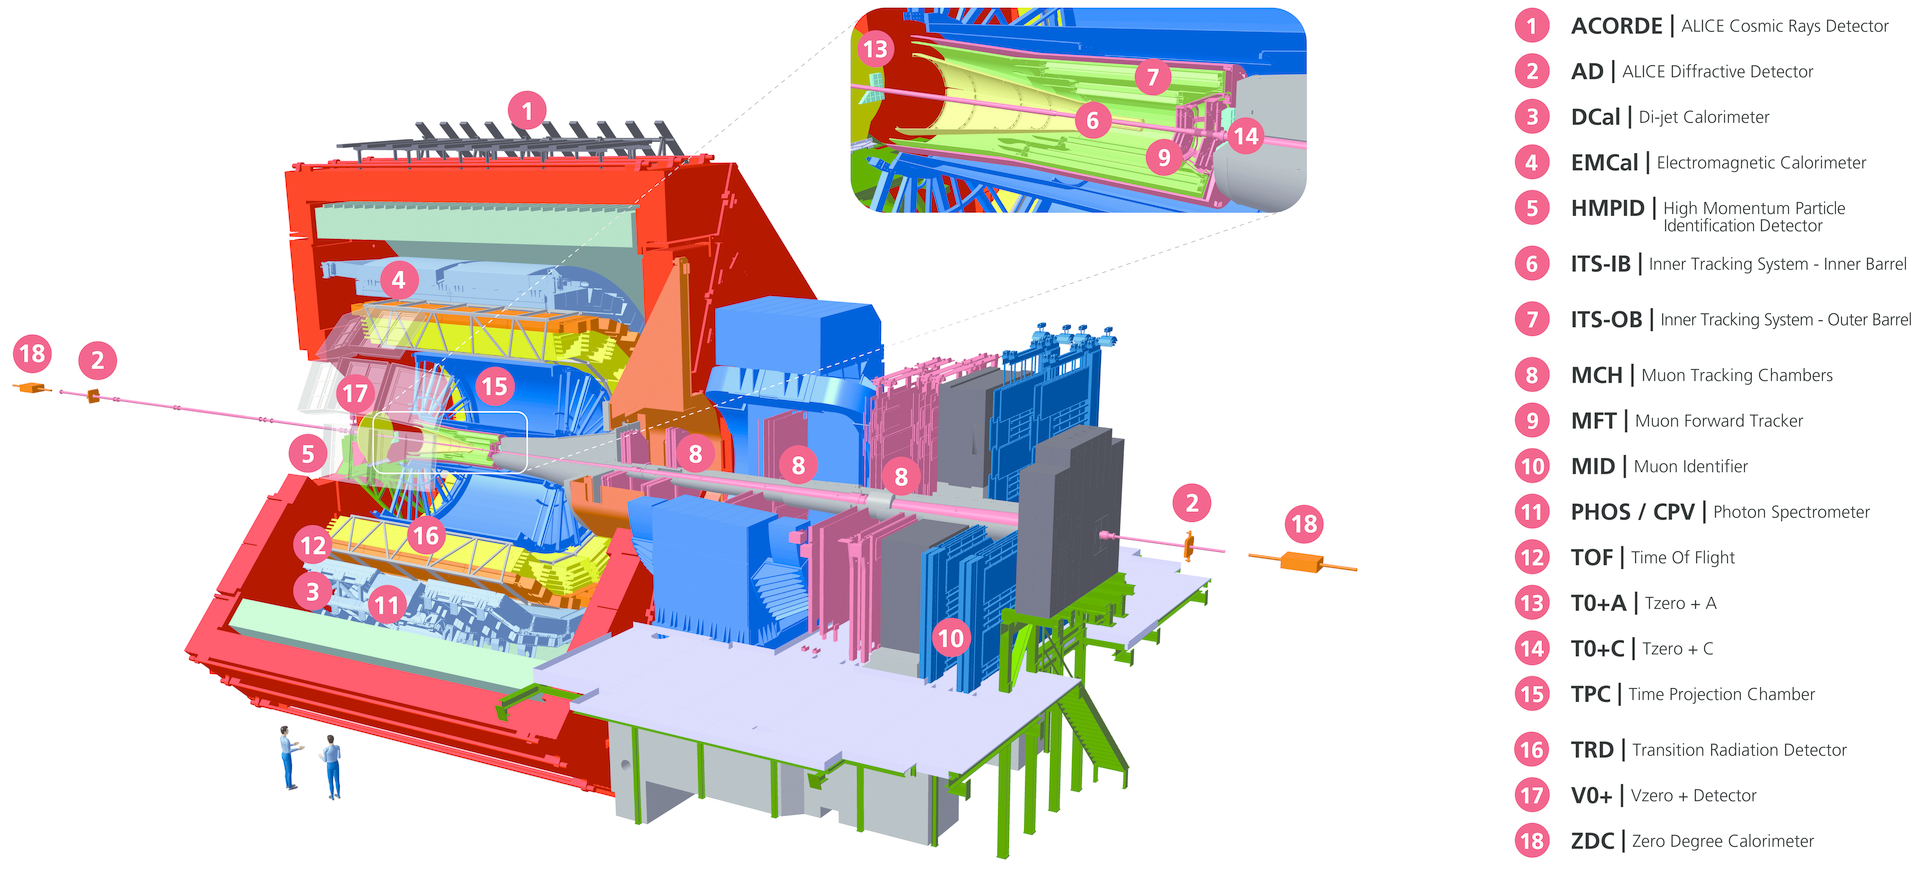
\includegraphics[width=\textwidth]{Figures/Chapter 3/ALICE_Scheme.png}
    \caption{The ALICE experimental apparatus. The top right panel shows a zoom of the ITS, T0-A, T0-C and MFT detectors. Figure from ALICE figure repository~\cite{ALICE_figures}.}
    \label{fig:ALICE}
\end{figure}

The ALICE coordinate system is a right-handed system with the $z$-axis pointing along the beam direction, in the direction away from the muon arm, the $y$-axis pointing vertically up, and the $x$-axis pointing horizontally towards the center of the LHC. The nominal interaction point is the origin of the coordinate system. The two sides of the detector along the beam axis are referred to as the C-side, where the muon arm is positioned, and the A-side, where the FV0 is positioned. The polar angle $\theta$ is defined with respect to the $z$-direction and $\varphi$, the azimuthal angle, increases counter-clockwise
starting from the $x$-axis towards the CMS side.


The central barrel is enclosed in the L3 solenoid, which has an internal length of 12.1~m and a radius of 5.75~m, providing a magnetic field of 0.5~T. The L3 experiment was a detector at the Large Electron-Positron Collider (LEP) at CERN~\cite{Myers:1991ym}, which operated from 1989 to 2000, and was built in the cavern where ALICE is now located. The central barrel detector system is designed for efficient tracking in the high track-density environment of heavy-ion collisions, covering transverse momenta from $\sim100~\mevc$ to $\sim100~\gevc$ with excellent hadron and electron identification capabilities. It is also capable of the reconstruction of primary and secondary vertices with a resolution $\sim\SI{40}{\micro\meter}$. This allows for precise measurements of heavy-flavour hadrons, which typically decay at a distance of $\sim\SI{100}{\micro\meter}$ from the primary vertex. The L3 magnet hosts the Inner Tracking System (ITS), the Time Projection Chamber (TPC), the Transition Radiation Detector (TRD), the Time-Of-Flight (TOF) detector, the High-Momentum Particle Identification Detector (HMPID), and the Electromagnetic Calorimeter (EMCal). The central barrel also includes forward detectors such as the Muon Forward Tracker (MFT) and the Fast Interaction Trigger (FIT). The muon detectors cover the forward pseudorapidity range $-4.0 < \eta < -2.5$ and are made of absorbers, a large dipole magnet, planes of triggering Resistive Plate Chambers (RPC) and tracking multiwire proportional chambers (MWPC).

In the following sections, the main components of the ALICE detector are described in detail, following the path of a particle produced at mid-rapidity. The upgrades of the ALICE detectors during the LHC Long Shutdown 2 will be highlighted.

\subsection{ALICE upgrades overview}
The ALICE detector underwent a major upgrade during the LHC Long Shutdown~2, between 2019 and 2021, which renewed the experiment, now referred to as ALICE~2. The upgrade aimed at significantly improving the capabilities of ALICE to probe the QGP with heavy-flavour quarks, and enabling completely new measurements of the thermal emission of dielectron pairs. To achieve these goals, the ALICE detector was improved by enhancing the tracking capabilities of the central barrel detectors and increasing the readout rate of the detectors to expand the collected data sample. The Inner Tracking System (ITS) was replaced with a new detector, the ITS-2, a thinner and lighter detector with the first layer closer to the interaction point, which improves the pointing resolution by a factor of 3 in the transverse direction and a factor 6 in the longitudinal direction, as shown in Fig~\ref{fig:ITS_res}.

\begin{figure}[htb]
    \centering
    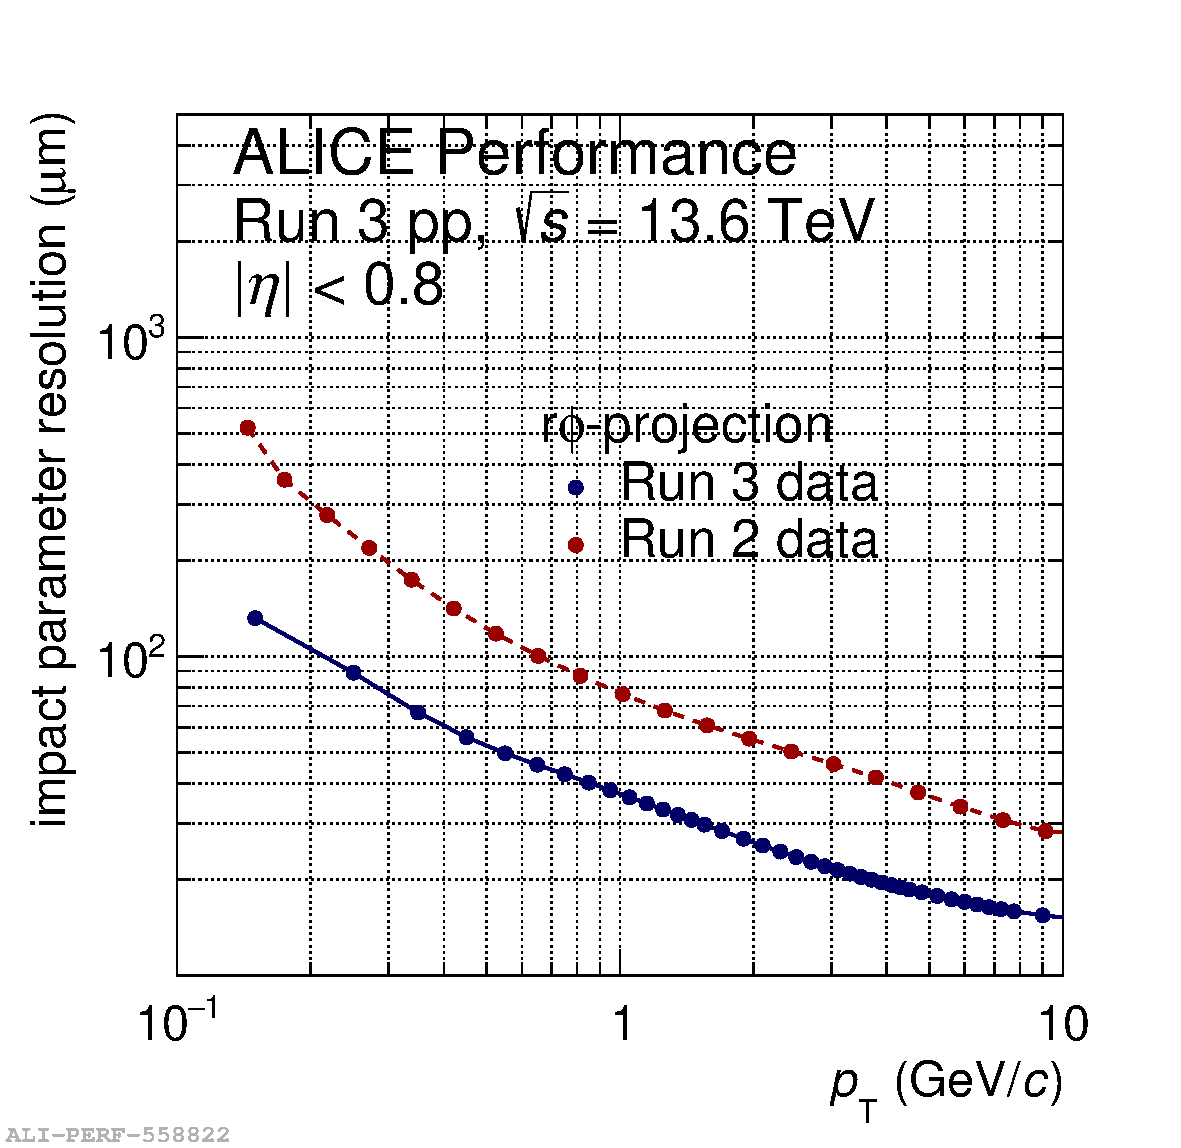
\includegraphics[width=0.7\textwidth]{Figures/Chapter 3/sigmadcaxy_run2vsrun3data_qm.pdf}
    \caption{Impact parameter resolution in $r\phi$ as a function of \pt in pp collisions at \thirteen from Run 3 data compared with the same quantity measured in collisions at $\sqrt{s} = 13$~\tev from Run 2 data. Figure taken from ALICE figure repository~\cite{ALICE_figures}.}
    \label{fig:ITS_res}
\end{figure}

The upgrade strategy for the enhanced readout rate is based on the LHC plans to increase the luminosity of Pb--Pb collisions progressively after the LHC Long Shutdown 2, eventually reaching an interaction rate of about 50~kHz (from less than 1~kHz during LHC Run~1 and 2 data-taking periods), i.e. instantaneous luminosity of $\mathcal{L} = 6\times10^{27}~\mathrm{cm}^{-2}~\mathrm{s}^{-1}$. At these high interaction rates, each TPC drift time period of $\sim\SI{100}{\micro\second}$ will contain on average 5 Pb--Pb events. It was therefore decided to use a continuous, untriggered readout strategy. With the MWPC used in ALICE~1 for the TPC readout, the ion backflow into the drift region had to be suppressed by active gating, limiting the readout rate to about 700 Hz for Pb--Pb collisions. This is overcome in ALICE~2 by using a readout based on Gas Electron Multiplier (GEM) foils, which reduce the ion backflow and resulting space charge in the TPC to a level that can be corrected for while operating the detector with Pb--Pb interaction rates up to 50 kHz. 

To synchronise the continuous data stream across all readout and processing branches, the data stream is divided into time frames (TF) of nominal length of 128 LHC orbits ($\sim11$~ms). Each TF is subdivided into heartbeat frames (HBF) with a length corresponding to an orbit of $\sim\SI{89.4}{\micro\second}$. The detector data are time stamped with a precision of an LHC bunch crossing of 25~ns. 

The Online-Offline (\osq) software framework has been developed to allow for distributed and efficient processing of this unprecedented amount of data. Because of the continuous readout in Run~3, the vertex-to-track association is no longer unambiguous. Therefore, in place of the analysis data model used in Runs~1 and 2, based on the hierarchical structure of the "event content", the analysis data model for Run~3 is based on a columnar data format, where collisions and tracks are represented as separate tables, connected by an index. This maps naturally on a "flattened" structure-of-arrays data format. Hence, the columnar data format provided by Apache Arrow~\cite{ApacheArrow} was chosen. The new framework ensures a unified and coherent computing environment from data taking up to analysis. Throughout all stages of the data processing, the timeframe represents the minimal processing unit. 

The result of asynchronous reconstruction is the Analysis Object Data (AOD) format, with the best calibration available. During processing the content of an AOD timeframe is kept contiguously in shared memory allowing efficient application of parallel execution and pipelining. AODs are stored as ROOT trees, exploiting their columnar storage format. The ROOT trees are then used to perform physics analyses. 

\subsection{Inner Tracking System}
The Inner Tracking System (ITS) is the innermost detector of the ALICE apparatus, and is designed to provide precise tracking and vertexing capabilities in the high-multiplicity environment of heavy-ion collisions. The ITS upgrade is one of the key improvements of the ALICE~2 detector. The ITS~1 was a six-layer silicon detector, with two layers of Silicon Pixel Detectors (SPD), two layers of Silicon Drift Detectors (SDD), and two layers of Silicon Strip Detectors (SSD). The ITS~1 was replaced by the ITS~2, which brought a plethora of improvements: i. a new beryllium beam pipe with an outer radius reduced from 28~mm to 18~mm allows for an innermost detector layer closer to the interaction point, from 39~mm to 22.4~mm; ii. an increased granularity for all layers, which are now silicon pixel detectors with a cell size of $\SI{29.24}{\micro\meter}\times\SI{26.88}{\micro\meter}$; iii. the number of layers for the inner barrel was increased from two to three, raising the total number of layers from six to seven; iv. the material budget was reduced to $0.36\%~X_0$ ($1.10\%~X_0$) per layer for the innermost (outer) layers. A schematic view of the ITS~2 is presented in Fig.~\ref{fig:ITS}, while the main layout parameters are summarised in Table~\ref{tab:ITS2_params}.

\begin{figure}
    \centering
    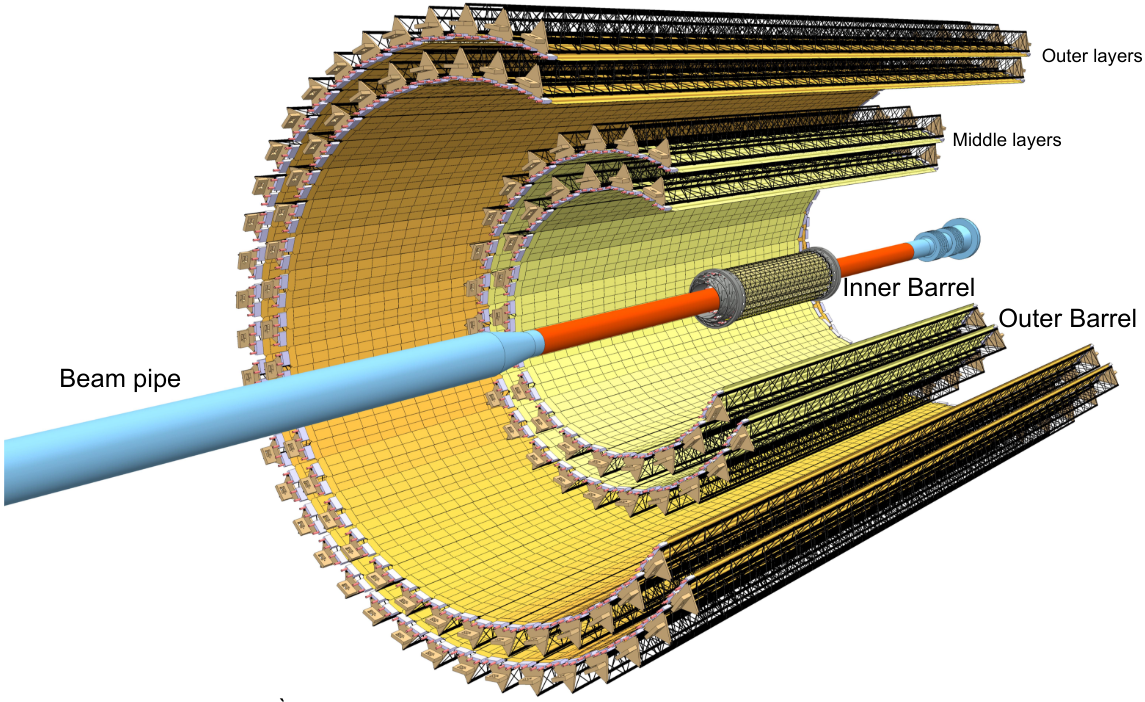
\includegraphics[width=0.7\textwidth]{Figures/Chapter 3/ITS_Scheme.png}
    \caption{Schematic view of the ALICE ITS-2. Figure taken from Ref.~\cite{ALICE:2023udb}.}
    \label{fig:ITS}
\end{figure}

\begin{table}[t]
    \centering
    \caption{Main layout parameters of the new ITS2. Taken from Ref.~\cite{ALICE:2023udb}.}
    \begin{tabular}{c|ccccc}
    \toprule
    Layer no. &	Average&	Stave&	No. of &No. of &Total no.\\
    &	radius&length&staves&HICs/	&of chips\\
    &	(mm)&(mm)& &stave	&\\
    
    \midrule
    0	&23 & 271 & 12 & 1&108\\
    1	&31 & 271 & 16	& 1&144\\
    2	&39 & 271 & 20	& 1&180\\
    3	&196 & 844 & 24 & 8	&2688\\
    4	&245 & 844 & 30 & 8	& 3360\\
    5	&344 & 1478	&42 & 14 &	8232\\
    6	&393 & 1478	& 48 & 14 &	9408\\
    
    \bottomrule
    \end{tabular}
    \label{tab:ITS2_params}
\end{table}

In addition, the ITS~2 uses ALPIDE~\cite{AglieriRinella:2017lym} chips, i.e., Monolithic Active Pixel Sensors~\cite{Snoeys:2014daa} (MAPS) implemented in a 180~nm CMOS technology for imaging sensors provided by TowerJazz~\cite{Senyukov:2013se}.

MAPS are an evolution of the hybrid pixel sensors which have been widely used in the past by several experiments~\cite{ALICE:2008ngc,CMS:1997tlf,Aad:2008zz,Bediaga:2013tje}. Hybrid pixel sensors are made of an active layer, typically made of silicon, and a readout layer, connected to the active layer by bump-bonding. On top of being expensive and complex, the bump-bonding operation introduces additional material in the detector, which increases the material budget of the detector. MAPS, on the other hand, are monolithic sensors, where the active layer and the readout layer are integrated into the same silicon wafer. This significantly reduces the material budget of the detector. The ALPIDE chip is a 15~mm$\times$30~mm chip, with a pixel size of $\SI{29.24}{\micro\meter}\times\SI{26.88}{\micro\meter}$, and a total of 512$\times$1024 pixels. Each pixel cell contains a sensing diode, a front-end amplifier and a shaping stage, a discriminator, and a digital section. The digital section includes a multi-event buffer with three hit storage registers and a pixel mask register. At the time of writing this Thesis, the ITS~2 is the largest-scale application of MAPS in a high-energy physics experiment.

\subsection{Time Projection Chamber}
\begin{figure}
    \centering
    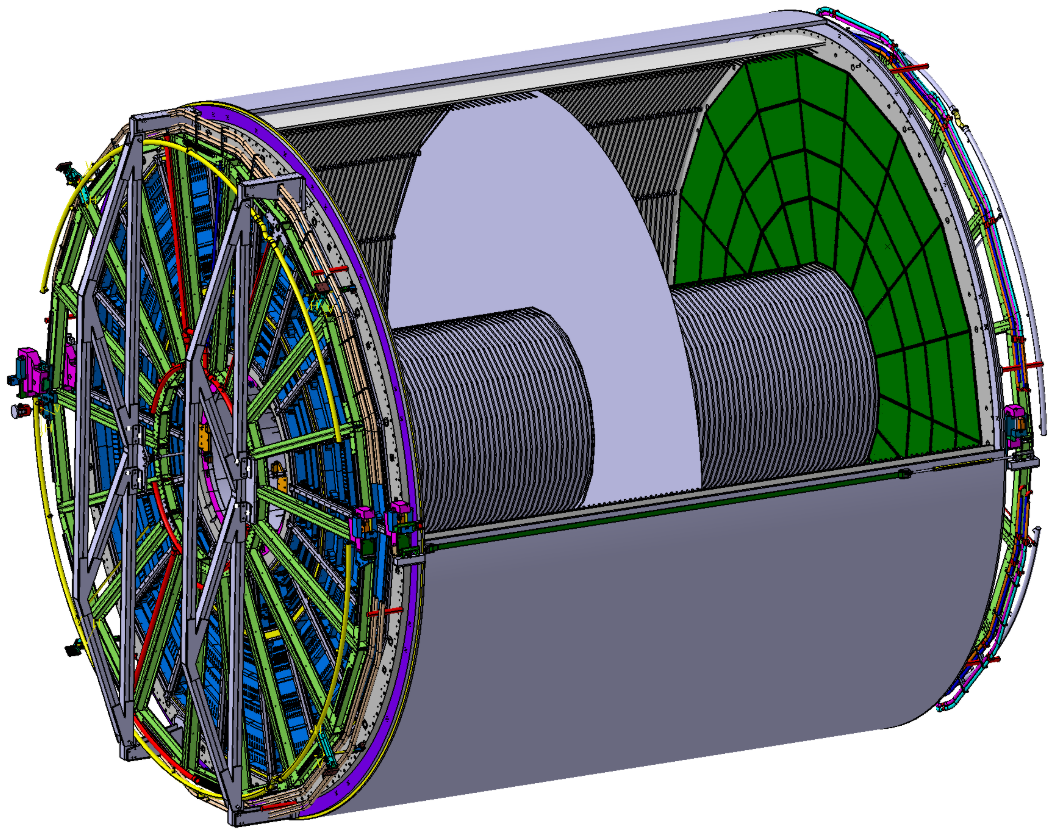
\includegraphics[width=0.7\textwidth]{Figures/Chapter 3/TPC_Scheme.png}
    \caption{Schematic view of the ALICE TPC. Figure taken from Ref.~\cite{ALICE:2023udb}.}
    \label{fig:TPC}
\end{figure}
The Time Projection Chamber is the main tracking detector of the ALICE experiment, and is designed to provide precise \pt measurements and particle identification via $\de E/\de x$ of charged particles. The TPC is a large cylindrical detector with a length and outer diameter of about 5 m, resulting in a volume of 88~m$^3$ filled with a gas mixture of Ne-CO$_2$-N$_2$ (90-10-5). It covers a symmetric pseudorapidity interval around midrapidity ($\lvert\eta\rvert < 0.9$) at full azimuth. The field cage has a high-voltage (100~kV) electrode in its center, which divides the active volume into two halves. The inner diameter of the central field cage drum is 114~cm, providing the necessary space for the installation of the ITS.  Each of the two endplates houses 18 inner and outer readout chambers (IROCs and OROCs), which are arranged in pairs to form 18 equal azimuthal sectors.

During Runs~1 and 2, the readout chambers were based on MWPCs, which have to be operated with an active ion gating grid in order to prevent the ions produced in the amplification region from reaching the active drift volume, which could lead to space-charge distortions. The ambitious physics program of the ALICE experiment requires the elimination of the intrinsic trigger rate limitation to about 3 kHz of the original MWPC-based TPC, imposed by the operation of the active ion gating grid.

Operating the TPC at a collision rate of 50 kHz implies that on average five collision events pile up within the TPC readout time window of about $\sim\SI{100}{\micro\second}$. This excludes triggered operation and defines the need for continuous readout, requiring the exploitation of gas amplification techniques capable of providing sufficient ion blocking without an active gate. At the same time, the readout system must ensure that the $\de E/\de x$ resolution of the TPC is preserved.

GEMs~\cite{Sauli:1997qp} represent a valid solution to overcome the limitations of MWPCs. Sufficient ion blocking can be achieved by stacking four GEMs using standard (S, \SI{140}{\micro\meter}) and large (LP, \SI{250}{\micro\meter}) hole pitch in an S-LP-LP-S configuration and by adjusting the gain share among the four layers. The latter optimisation allows for efficiently blocking the ions, most of which are produced in the last amplification step, i.e. the closest to the readout pad. A careful choice of hole patterns is made to avoid the accidental alignment of holes in subsequent layers. 

Thanks to this design, the detector is capable of satisfying the requirements for Run~3 operation, with an ion backflow below 2\% and a local energy resolution at the $^{55}$Fe-peak below 14\%.

\subsection{Time-of-Flight}
The TOF detector is a large area detector covering the central pseudo-rapidity region ($\lvert\eta\rvert < 0.9$), extending from an inner radius of 370~cm to an external one of 399~cm. Its main purpose is the particle identification in the intermediate momentum range, achieving a $\pi$/K and K/p separation better than 3 times the time-of-flight resolution below about 2.5~\gevc for pions, and up to 4~\gevc for protons. The TOF detector is built with a modular structure corresponding to 18 sectors in $\varphi$ and five modules along the beam direction. It is based on Multi-gap Resistive Plate Chambers (MRPCs)~\cite{Wang:2020iwn}, which are capable of providing a time resolution of about 40~ps~\cite{ALICE:2008ngc}. The gas mixture used in the MRPCs is $\mathrm{C_2H_2F_4 (90\%), i\text{-}C_4H_{10} (10\%), SF_6 (5\%)}$, which proved to be a good solution as no significant ageing effects were observed after 3.5 times the dose foreseen in the first 10 years of operation.

Together with the ITS and TPC, the TOF is the detector in charge of providing event-by-event identification of large samples of pions, kaons, and protons. The mass of a given particle is estimated from the measurement of its time-of-flight:
\begin{equation}
    m = p \cdot \sqrt{\left(\frac{t_\mathrm{flight}}{L}\right)^2 - 1}\quad ,
\end{equation} 
where $p$ is the particle's momentum, measured from the curvature of its trajectory, $t_\mathrm{flight}$ is the time-of-flight, and $L$ is the track length. \textcolor{red}{si trascura la curvatura?} The time-of-flight is evaluated as the difference between the time of arrival of the particle at the TOF $t_\mathrm{hit}$ and the time of the collision $t_0$, estimated using a timing signal from the FT0 detector, which is described in Sec.~\ref{subsec:FIT}: $t_\mathrm{flight} = t_\mathrm{hit} - t_0$.

\subsection{Fast Interaction Trigger}\label{subsec:FIT}
The Fast Interaction Trigger (FIT) serves as the main forward trigger, luminometer, and interaction-time detector. It also provides an initial indication of the vertex position and determines the multiplicity, centrality, and reaction plane of heavy-ion collisions. The FIT consists of five distinct detector stations, positioned at different locations along the beam line: the FT0 (-A and -C), the FV0, and the FDD (-A and -C). An illustration of the FIT is shown in Fig.~\ref{fig:FIT}.

\begin{figure}[htb]
    \centering
    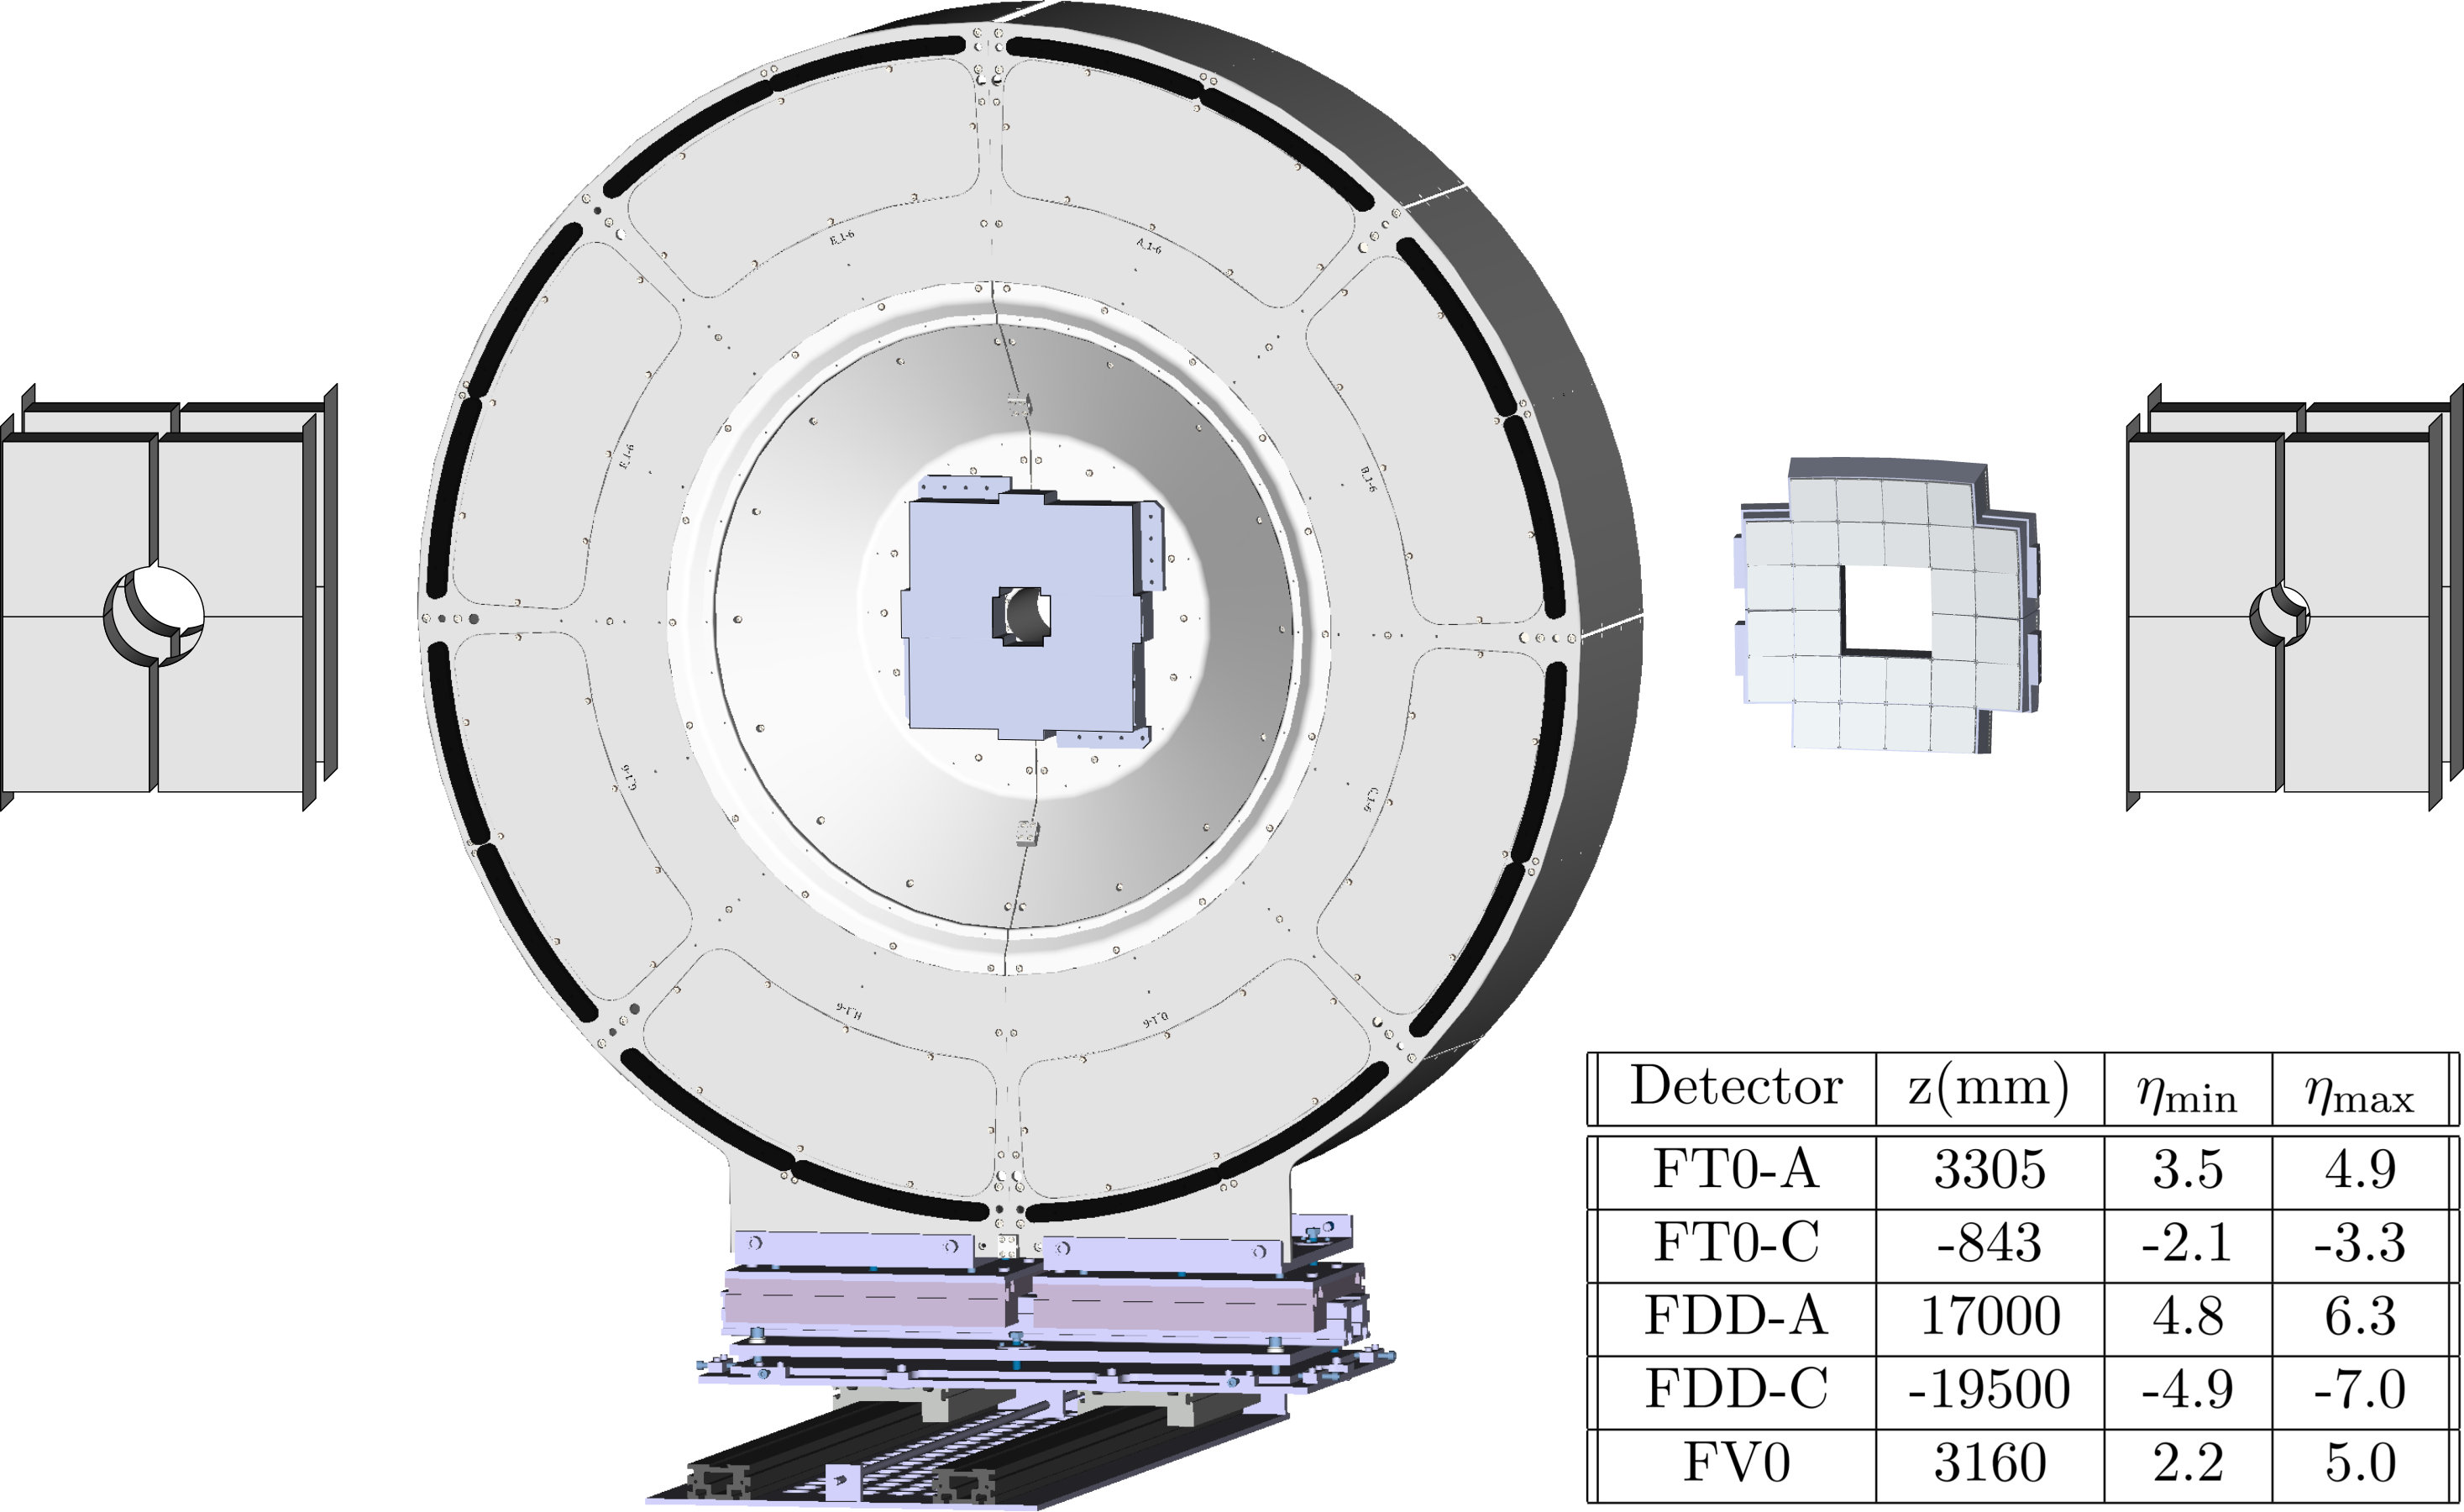
\includegraphics[width=0.7\textwidth]{Figures/Chapter 3/FIT_Scheme.png}
    \caption{View of the FIT detectors illustrating the relative sizes of each component. From left to right, the FDD-A, FT0-A, FV0, FT0-C, and FDD-C are shown. The FT0-A and FV0 systems have a common mechanical support: the former is the small quadrangular structure in the centre of the large, circular FV0 support. The inset table lists the distance from the interaction point and the pseudorapidity coverage for each component. Figure taken from Ref.~\cite{ALICE:2023udb}.}
    \label{fig:FIT}
\end{figure}

\subsubsection{FT0}

The FT0 is made of two arrays of quartz Cherenkov radiators, FT0-A and FT0-C, coupled to MicroChannel Plate-based photomultipliers (MCP). Its main task is to determine the vertex position with an accuracy of a few centimeters, and to provide the interaction time with the precision needed by the TOF system for event-by-event particle identification. An optimal time resolution ($<50$~ps) is therefore required. The FT0-A is located at 3.3~m from the nominal interaction point, while the FT0-C is only 84~cm from the interaction point. To provide a reliable indication of the time of a collision, the FT0-C support has a convex shape, to ensure that each of the 112 quartz radiators is positioned at a distance of 84 cm from the nominal interaction point. On the contrary, the FT0-A is characterised by a planar geometry, made of 96 quartz radiators. To achieve the best possible timing resolution, the signal path from each MCP anode to the front-end electronics has the same length. The intrinsic time resolution of each quadrant is $\sigma_t \sim 13$~ps

\subsubsection{FV0}
The FV0 is a large, segmented scintillator disk. It achieves a single MIP time resolution of about 200~ps with a very uniform response across the entire detection surface thanks to its light collection scheme, shown in Fig.~\ref{fig:FV0}. The active element of FV0 is a 4~cm-thick plastic scintillator divided into five concentric rings of equal pseudorapidity coverage. The outer diameter of the largest ring is 144~cm and the inner diameter of the smallest is 8~cm. The four inner rings are subdivided into eight sectors of 45 degrees each, while the outermost ring, due to its large area, has 16 sectors. A grid of equal-length fibers is attached to the back side of the scintillator, where they are attached to the photomultiplier tubes (PMTs). Each sector is read out by an independent PMT to provide a minimum bias and multiplicity trigger, when coupled to the FT0 information.

\begin{figure}[htb]
    \centering
    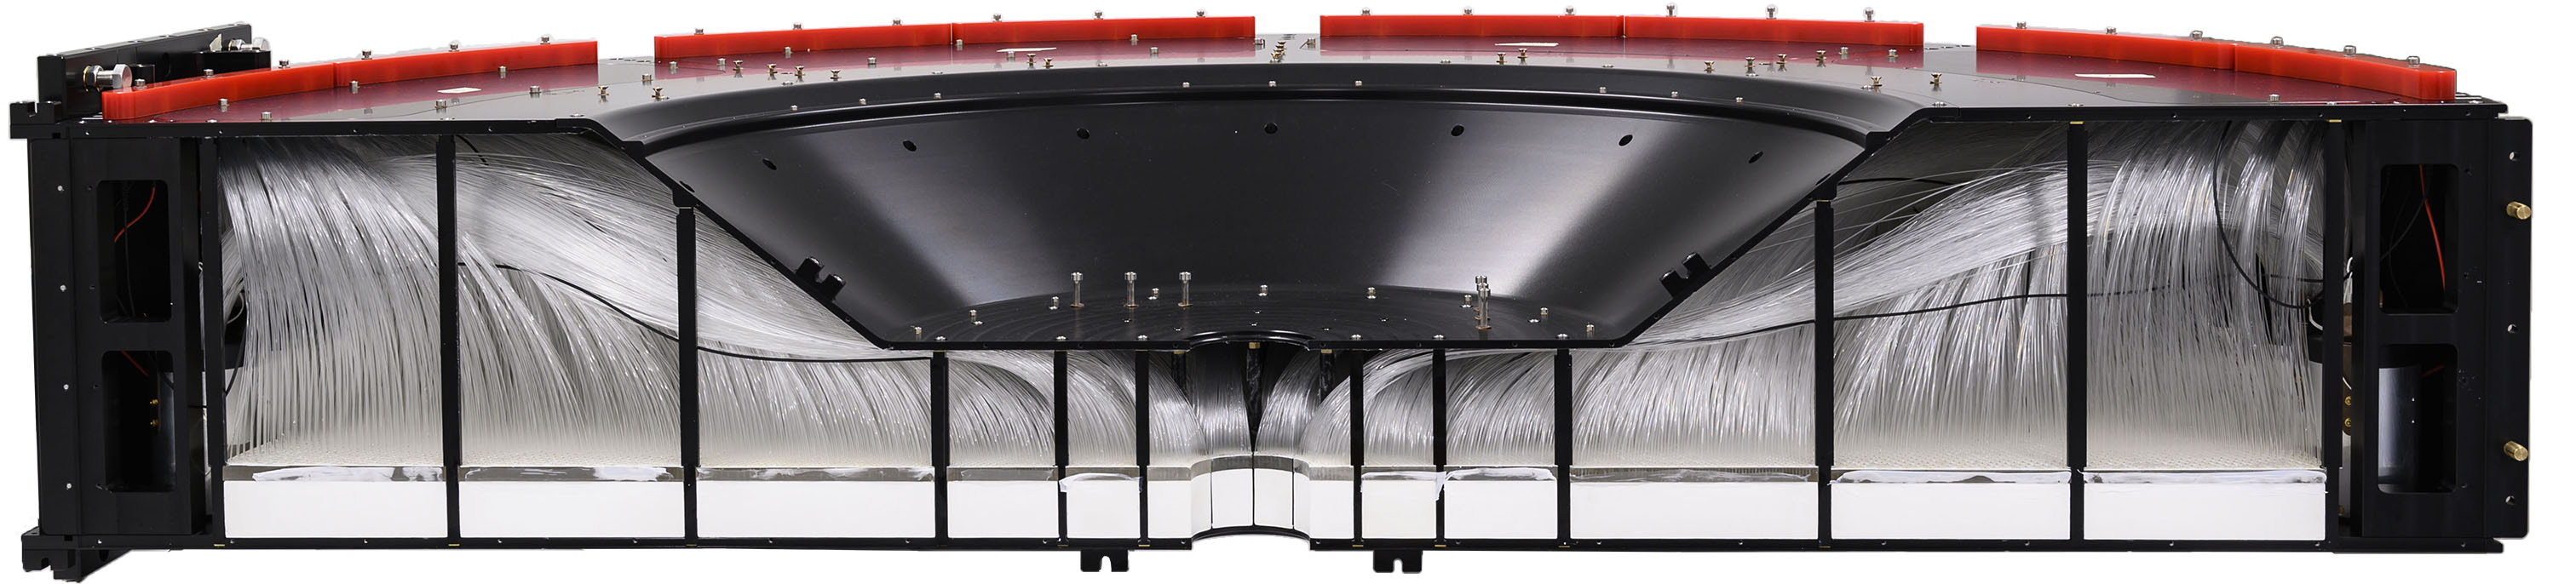
\includegraphics[width=0.7\textwidth]{Figures/Chapter 3/FV0_Scheme.jpg}
    \caption{Photograph of one half of the FV0 detector. Figure taken from Ref.~\cite{ALICE:2023udb}.}
    \label{fig:FV0}
\end{figure}

\subsubsection{FDD}
The FDD is made of two similar arrays, FDD-A and FDD-C, surrounding the beam pipe on opposite sides of the nominal interaction point, and consisting of eight rectangular scintillator pads each, arranged into two overlapping layers of four sectors. A quadrant was removed from the innermost corner of each scintillator plate to allow for the passage of the beam pipe. Since the FDD covers a large pseudorapidity interval, and is sensitive to the presence of even a single MIP, it is an ideal system to tag interactions characterised by large rapidity gaps as those from photon-induced ultra-peripheral collisions or diffractive processes.
\setcounter{chapter}{3}
%\chapter{\texorpdfstring{\dpl\ and \ds\ reconstruction strategy in proton-proton collisions}{D+ and Ds+ reconstruction strategy in proton-proton collisions}}\label{chap:reconstruction}

\textcolor{red}{Aggiungere disegno decadimento}

Due to their mean proper decay lengths (\ct) of \SI{151.2}{\micro\meter} and \SI{309.8}{\micro\meter} respectively~\cite{pdg}, \ds\ and \dpl\ mesons and their charge conjugate cannot be directly detected by the ALICE detector, as they typically decay before reaching the detector. Consequently, their production is inferred through the reconstruction of their decay products. This analysis exploits their hadronic decays into $\ds (\dpl) \rightarrow \mathrm{\phi\pi^+ \rightarrow K^+K^-\pi^+}$ and their charge conjugates, with a branching ratio of $2.21\times10^{-2}$ ($2.69\times10^{-3}$)~\cite{pdg}. An additional hadronic decay channel of the \dpl meson with a larger BR of $9.38\times10^{-2}$~\cite{pdg} could be exploited~\cite{ALICE:2017olh}, but the reconstruction of the two D-mesons species in the same decay channel allows for the cancellation of many of the systematic uncertainties affecting the measurement, leading to a more precise \ds/\dpl production yield ratio measurement. The choice of reconstructing D mesons through their decays into an hadronic final state allows for the full reconstruction of the decay topology, therefore providing a more precise measurement, as semileptonic decays are affected by larger uncertainties due to the presence of neutrinos in the final state, which are not detected. In addition, the decay into the resonant $\phi(1020)$ state opens up the possibility of exploiting the invariant mass of the $\phi$ meson for the selection of the D-meson candidates.

\ds\ and \dpl\ mesons (and their charge conjugates) are reconstructed in three different steps: i. firstly, charged tracks are reconstructed at midrapidity ($\lvert\eta\rvert < 0.8$) exploiting the ITS and TPC detectors; ii. \ds\ and \dpl\ candidates are constructed by combining triplets of tracks with the appropriate charge signs, i.e., (+, --, +) for \ds\ and \dpl\ mesons, and (--, +, --) for their antiparticles; iii. finally, the \ds\ and \dpl\ candidates are selected by applying a set of topological, kinematical, and Particle-IDentification (PID)  selections. Given the large number of tracks produced in a pp collision, the vast majority of the constructed \ds\ and \dpl\ candidates are obtained from the combination of uncorrelated tracks, which do not originate from the same decay vertex. This results in a large \emph{combinatorial background}, which has to be suppressed in order to extract the signal of the D mesons. 

The spatial resolution capabilities of the ALICE detector described in Chapter~\ref{chap:ALICE} enable the separation of the secondary decay vertices of D mesons from the primary interaction vertex, which consents the development of an analysis based on the reconstruction and selection of secondary-vertex topologies characterised by relatively large separations from the primary interaction vertex. Furthermore, PID information can be exploited to improve the selection of the D mesons and their decay products and reduce the background.

Two distinct categories of D mesons emerge based on their production mechanisms: \emph{prompt} and \emph{non-prompt} (also referred to as \emph{feed-down}) D mesons. Decay vertices of feed-down D mesons are on average more displaced from the interaction vertex with respect to promptly-produced ones, due to the larger mean proper decay lengths of beauty hadrons (\ct $\sim$ 500 µm~\cite{pdg}) as compared to charm hadrons. Therefore, by exploiting selection criteria based on displaced decay-vertex topologies, it is possible not only to separate D mesons from the combinatorial background, but also enables the discrimination between feed-down and prompt D mesons.

\section{Data sample and event selection}
The analysis reported in this Thesis is performed on a dataset of pp collisions at a centre-of-mass energy of \thirteen, collected by the ALICE detector during the 2022 data-taking period. The data sample is collected using a Minimum-Bias trigger (the ``Sel8" trigger), which selects events which satisfy the requirement of having a signal coincidence in the FT0-A and FT0-C detectors. Furthermore, because it is observed that the readout of the TPC (which happens at the end of each TF) causes a drop in the track reconstruction efficiency, it was decided to exclude the collisions read out during the TPC readout (\emph{TF border} selection). An additional requirement is imposed on the vertex position along the beam axis, $\lvert z_{\mathrm{vtx}}\rvert<10$~cm, to ensure that the primary vertex is located within the region of the detector where the tracking efficiency is optimal. Of the total 59.2 billion collected events, only 54.7 billion have been analysed. Around 3\% of the events are rejected due to the minimum bias trigger, about 1\% due to the TF border selection, and 4\% of the events are rejected due to the requirement on the $z_{\mathrm{vtx}}$ position. A summary of the event selection is shown in Fig.~\ref{fig:EvSel}.


\begin{figure}[htb]
    \centering
    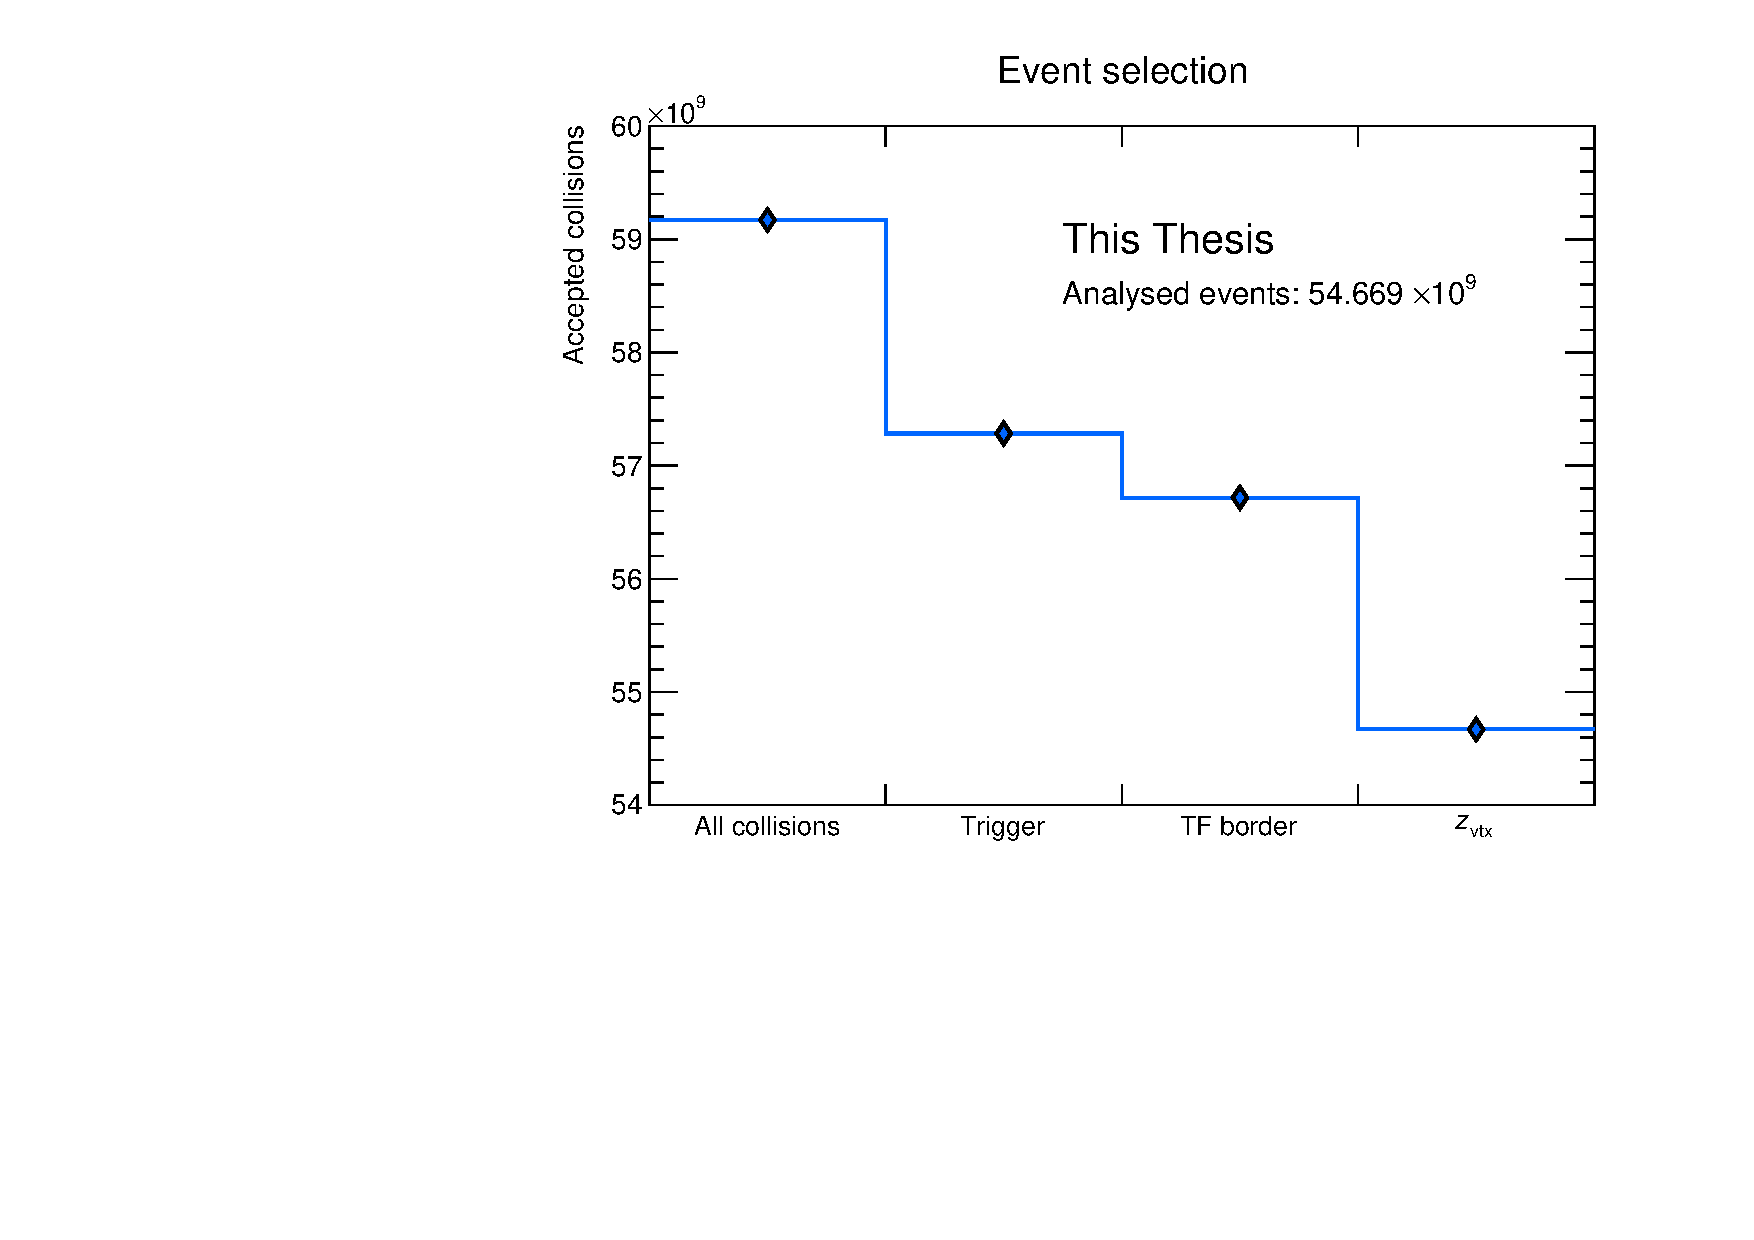
\includegraphics[width=0.7\linewidth]{Figures/Chapter 4/EventSelection.pdf}
    \caption{Summary of the event selection criteria applied to the data sample.}
    \label{fig:EvSel}
\end{figure}

\section{\texorpdfstring{\ds and \dpl reconstruction workflow}{Ds+ and D+ reconstruction workflow}}
The reconstruction of \ds and \dpl mesons is a complex process performed in many subsequent steps. As stated in Chapter~\ref{chap:ALICE}, the reconstructed data are stored in AOD format. This format contains essential information about the reconstructed tracks, which are parameterised at the innermost update point, i.e., the closest point to the primary vertex with a detected track signal. Since the track parametrisation is not the same for each track, as missing hits in the ITS can lead to different radii of the innermost update point, the tracks are propagated to the point of closest approach to the primary vertex, and their parameters are updated accordingly. Tracks are propagated in the \code{track-propagator} workflow, and only those passing a set of quality requirements are selected. 

Because of continuous readout, there exists the possibility that a single track is found to be compatible with multiple collisions (these tracks are named \emph{ambiguous tracks}). In the AOD files, the track is only associated with the first compatible collision. In order to increase the reconstruction efficiency, the \code{track-to-collision associator} workflow associates each track with all compatible collisions. This process significantly increases the reconstruction efficiency, especially for 2- or 3-body decaying particles.

For each considered collision, combinations of two or three tracks are built in the \code{track-index-skim-creator} workflow, which produces a table of track indices for combinations passing a set of loose selection criteria, which depend on the considered hadron species. Candidates for each particle species and their decay vertices are created in the \code{candidate-creator} workflow, and those passing the more stringent analysis selection criteria are flagged in the \code{candidate-selector} workflow. The \code{tree-creator} (\code{analysis-task}) workflow produces the final output of the analysis, which consists of a ROOT tree (several ROOT histograms) containing the properties of selected candidates.

\section{\texorpdfstring{\ds and \dpl decay-vertex reconstruction and selection}{Ds+ and D+ decay-vertex reconstruction and selection}}
 The decay vertex of the candidate is reconstructed through a minimisation of a $\chi^2$-like quantity, denoted as D:
\begin{equation*}
    D = \sqrt{\sum_{i=1}^3 \left[\left(\frac{x_i-x_0}{\sigma_{x_i}}\right)^2 + \left(\frac{y_i-y_0}{\sigma_{y_i}}\right)^2 +\left(\frac{z_i-z_0}{\sigma_{z_i}}\right)^2\right]}\quad ,
\end{equation*}
where ($x_i,y_i,z_i$) and ($\sigma_{x_i},\sigma_{y_i},\sigma_{z_i}$) represent the position and the uncertainty of the i-th track at the point of closest approach, respectively, while ($x_0,y_0,z_0$) denotes the position of the reconstructed vertex. The invariant mass and momentum of the \ds\ and \dpl\ candidates are computed from the energy and momentum of the measured tracks evaluated at the point of closest approach to the decay vertex. The momentum of the candidate is defined as the sum of the momenta of the three tracks. For the invariant mass computation, the kaon mass is always assigned to the track with opposite charge sign with respect to the D-meson candidate (\emph{opposite-sign track}). For the two \emph{like-sign tracks}, the two pion-kaon mass hypothesis combinations \big(i.e. ($\mathrm{K^+K^-\pi^+}$) and ($\mathrm{\pi^+K^-K^+}$) for positively charged candidates\big) are considered. 

A lot of triplets can be built from the tracks produced in a pp collision, and this number grows even more in a Pb--Pb collision, where the charged-particles multiplicity is much larger. Thus, many \ds- and \dpl-meson candidates are created, the vast majority of them being combinatorial background. To increase the signal-over-background ratio and the statistical significance of the measurement, tight selections are required. The analyses presented in this Thesis exploit several selection criteria, which can be divided into:
\begin{enumerate}[i]
    \item Track-quality selections
    \item Selections based on the decay topology and kinematics
    \item Particle identification of the decay products
\end{enumerate}
In the following, the applied selections are described in more detalis

\subsection{Track-quality selections}
Only tracks that successfully pass strict quality and kinematic requirements are considered eligible for inclusion in the construction of \ds- and \dpl-meson candidates. In particular, only ITS-TPC tracks with at least 70 (out of a maximum of 159) track-associated space points in the TPC, and a crossed rows (i.e., total number of hit TPC pad rows) over findable clusters (i.e., pad rows which could potentially be hit, given the track's trajectory) ratio of at least 0.8 are selected. To improve the vertex reconstruction procedure, at least one hit in the 3 innermost layers of the ITS, which compose the ITS inner barrel, was required.

Secondary vertices of \ds- and \dpl-meson candidates are constructed using tracks having $\lvert\eta\rvert < 0.8$ and $\pt > 0.3$~\gevc. A track-quality requirement of $\chi^2$ per TPC cluster smaller than 4 has been applied. A cut on the daughter-track transverse impact parameter projection in the transverse plane $d_0^{xy}$ was applied, requiring $d_0^{xy} > \SI{25}{\micro\meter}$ for tracks with $\pt < 2~\gevc $. These selections limit the rapidity acceptance of D mesons, which steeply decreases for $\lvert y\rvert > 0.5$ at low \pt and for $\lvert y\rvert > 0.8$ for $\pt \gtrsim 5~\gevc$, as shown in Fig.~\ref{fig:RapidityAcceptance}. The applied track-quality selections criteria are summarised in Table~\ref{tab:trackSel}.

\begin{figure}[htb]
    \centering
    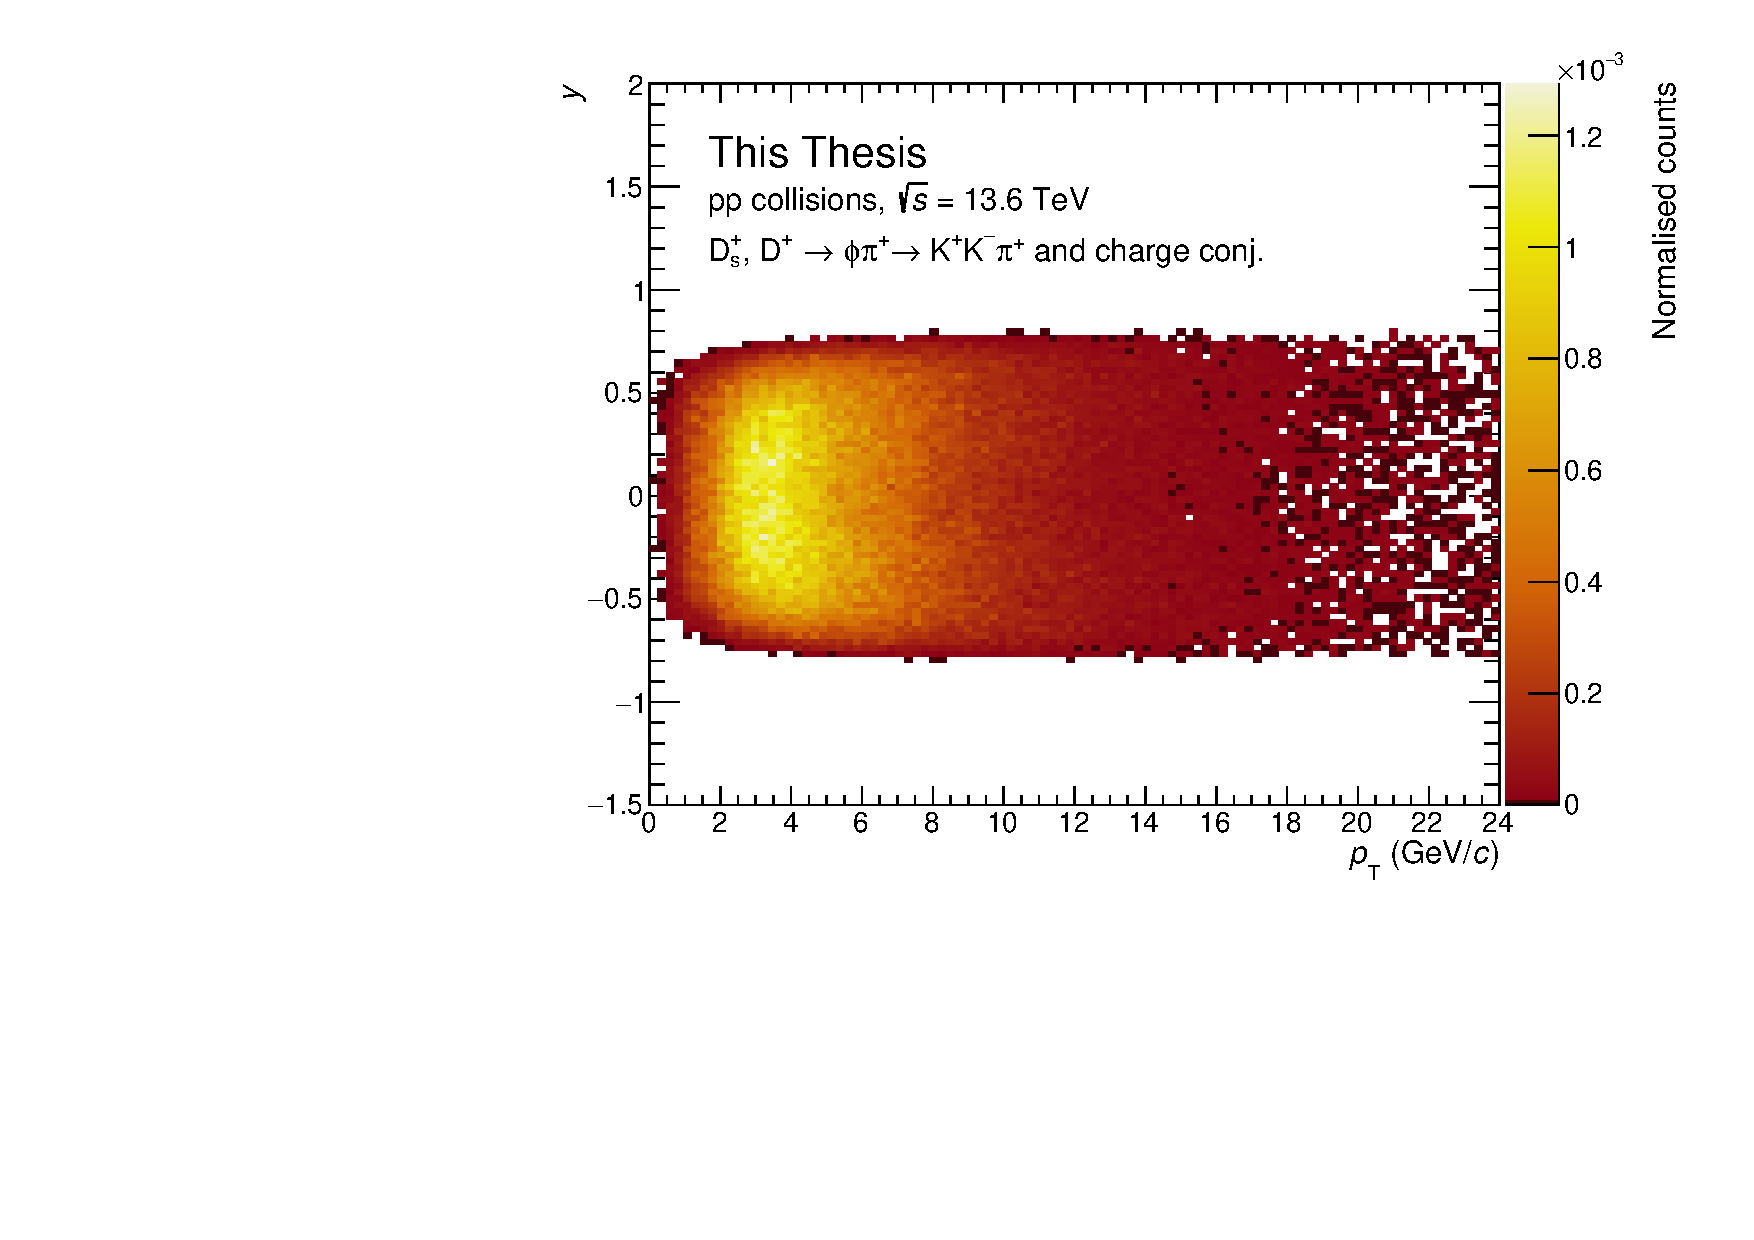
\includegraphics[width=0.7\linewidth]{Figures/Chapter 4/PtVsY.pdf}
    \caption{Rapidity and transverse momentum distribution of reconstructed \ds and \dpl mesons in pp collisions at \thirteen. \textcolor{red}{Sostituire con i dati.}}
    \label{fig:RapidityAcceptance}
\end{figure}

\begin{table}[htb]
  \begin{center}
    \begin{tabular}{c|c}
        \toprule
      Single-track selection & Value\\
      \midrule
      Number of TPC crossed-rows $>$  & 70 \\
      $\lvert\eta\rvert <$                         & 0.8\\
      $\pt >$                                       & 0.1 \gevc\\
      $\chi^2_\mathrm{TPC}$/TPC clusters $<$                     & 4\\
      $\chi^2_\mathrm{ITS}$/ITS clusters $<$                     & 36\\
      ITS matching & At least 1 cluster in L0, L1, L2\\
      \bottomrule
    \end{tabular}
    \caption{Applied single-track selection criteria }
    \label{tab:trackSel}
  \end{center}
\end{table}


\subsection{Topological selections}
\ds\ and \dpl\ mesons exhibit a displaced decay vertex topology, which can be used to separate the signal from the uninteresting combinatorial background. Moreover, promptly produced D mesons exhibit different topological features compared to feed-down D mesons, enabling further discrimination between the two production mechanisms. This differentiation potentially offers insights into beauty-quark production through the measurement of open-charm states. 

The topological selections are tuned as a function of the \pt\ in order to increase the signal-over-backroung and the statistical significance of the measurement. The different selections are presented herein. The corresponding distributions of variables are shown for the signal, which is divided into prompt and feed-down contributions and obtained from Monte Carlo simulations, as well as the combinatorial background, which is obtained from real data in a invariant-mass region away from the signal region, denoted as \emph{sidebands}.

\subsubsection{Decay Length}
\begin{figure}
    \centering
    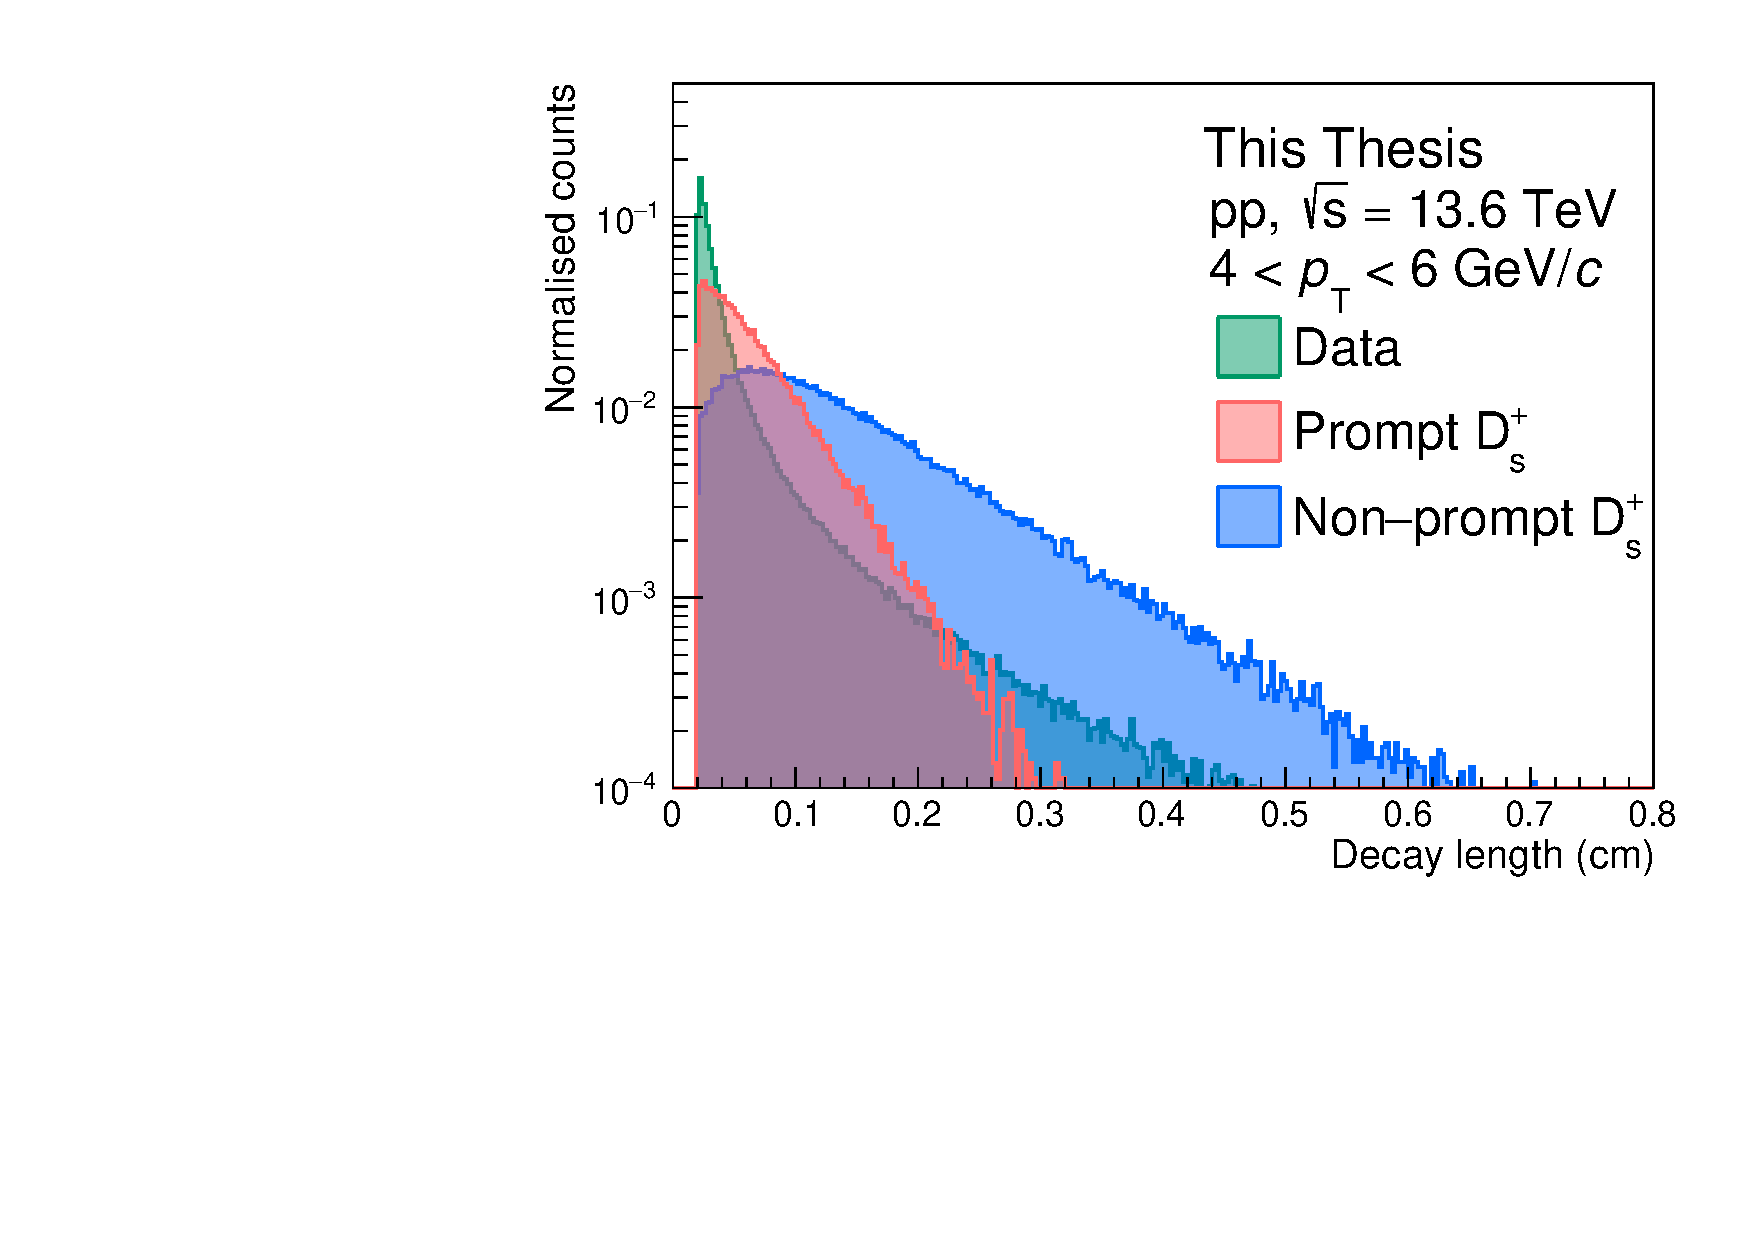
\includegraphics[width=0.48\linewidth]{Figures/Chapter 4/DecayLength.pdf}
    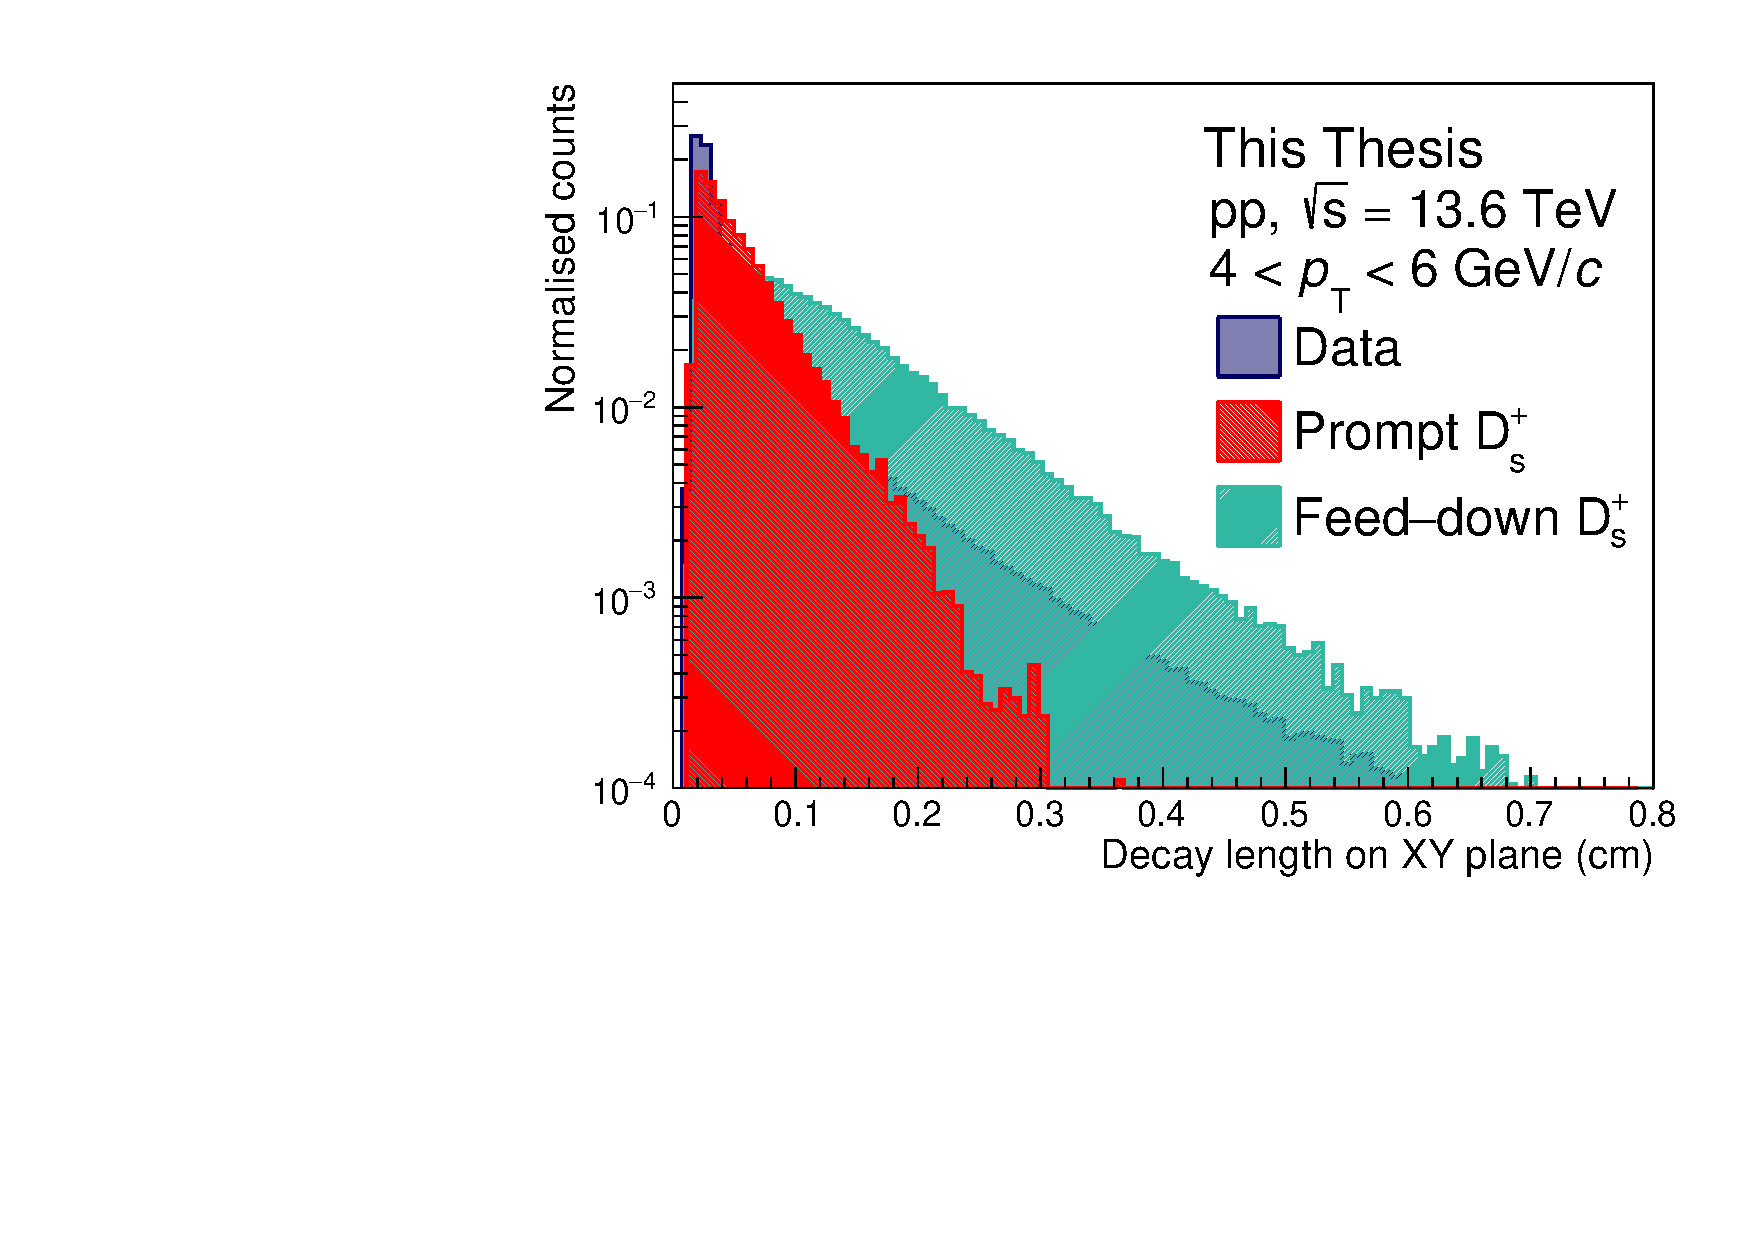
\includegraphics[width=0.48\linewidth]{Figures/Chapter 4/DecayLengthXY.pdf}
    \caption{Distributions of decay length (left panel) and its projection on the transverse plane (right panel)  for \ds mesons in pp collisions at \thirteen in the $4 < \pt < 6$~\gevc interval. The distributions
    are shown for prompt \ds mesons (blue), non-prompt \ds mesons (orange), and combinatorial background
    (green). For prompt and non-prompt \ds mesons, the distributions are taken from Monte Carlo
    simulations, whereas for combinatorial background they are taken from the data sidebands.}
    \label{fig:DecayLength}
\end{figure}
The decay length $L$ is defined as the distance between the primary and secondary vertices. It provides an approximation of the actual decay length of \ds\ and \dpl\ mesons, as the particle's curvature resulting from the motion in the presence of a magnetic field is not considered. However, given the small mean proper decay length of $\sim 150~(310)$ µm of \ds\ (\dpl) mesons, this effect can be neglected. 

This is one of the most important variables to distinguish between the signal and the combinatorial background, since the displaced topology of the signal shifts the decay length distribution towards greater values. Furthermore, since beauty-hadron decay verexes are not reconstructed, the measured decay lenght of non-prompt D-mesons also accounts for the decay lenght of their parent hadrons. As a consequence, the resulting decay lenght distribution for feed-down D-mesons is particularly shifted towards larger values, allowing for an easier separation of this production mechanism from the background. The distribution of the decay length also depends on the \pt\ of the D meson, because of the Lorentz boost which contributes to an increase in the travelled distance measured in the laboratory reference frame. Moreover, since the mean proper decay length of \dpl meson is about twice as large as that of the \ds meson, the decay length distribution of the former is shifted towards larger values. This allows for the discrimination of the two D-meson species.

In addition to the decay length, the projection of the decay length on the transverse plane can also be used to select \ds or \dpl signal. This variable is particularly useful as it exploits the better resolution of the transverse plane with respect to the longitudinal one of the ALICE experiment. Previous measurements of D mesons also leveraged the normalised decay length, defined as the ratio between the decay length and its uncertainty, to further improve the signal extraction. Although this variable demonstrated a good separation power, it was not used in this analysis, due to possible biases introduced by the uncertainty description in the Monte Carlo simulations.

The distributions of decay length and its projection on the trasverse plane are shown in Fig.~\ref{fig:DecayLength} for signal and combinatorial background candidates reconstructed in the $4 < \pt < 6$~\gevc interval. 

\subsubsection{Cosine of pointing angle}
\begin{figure}[tb]
    \centering
    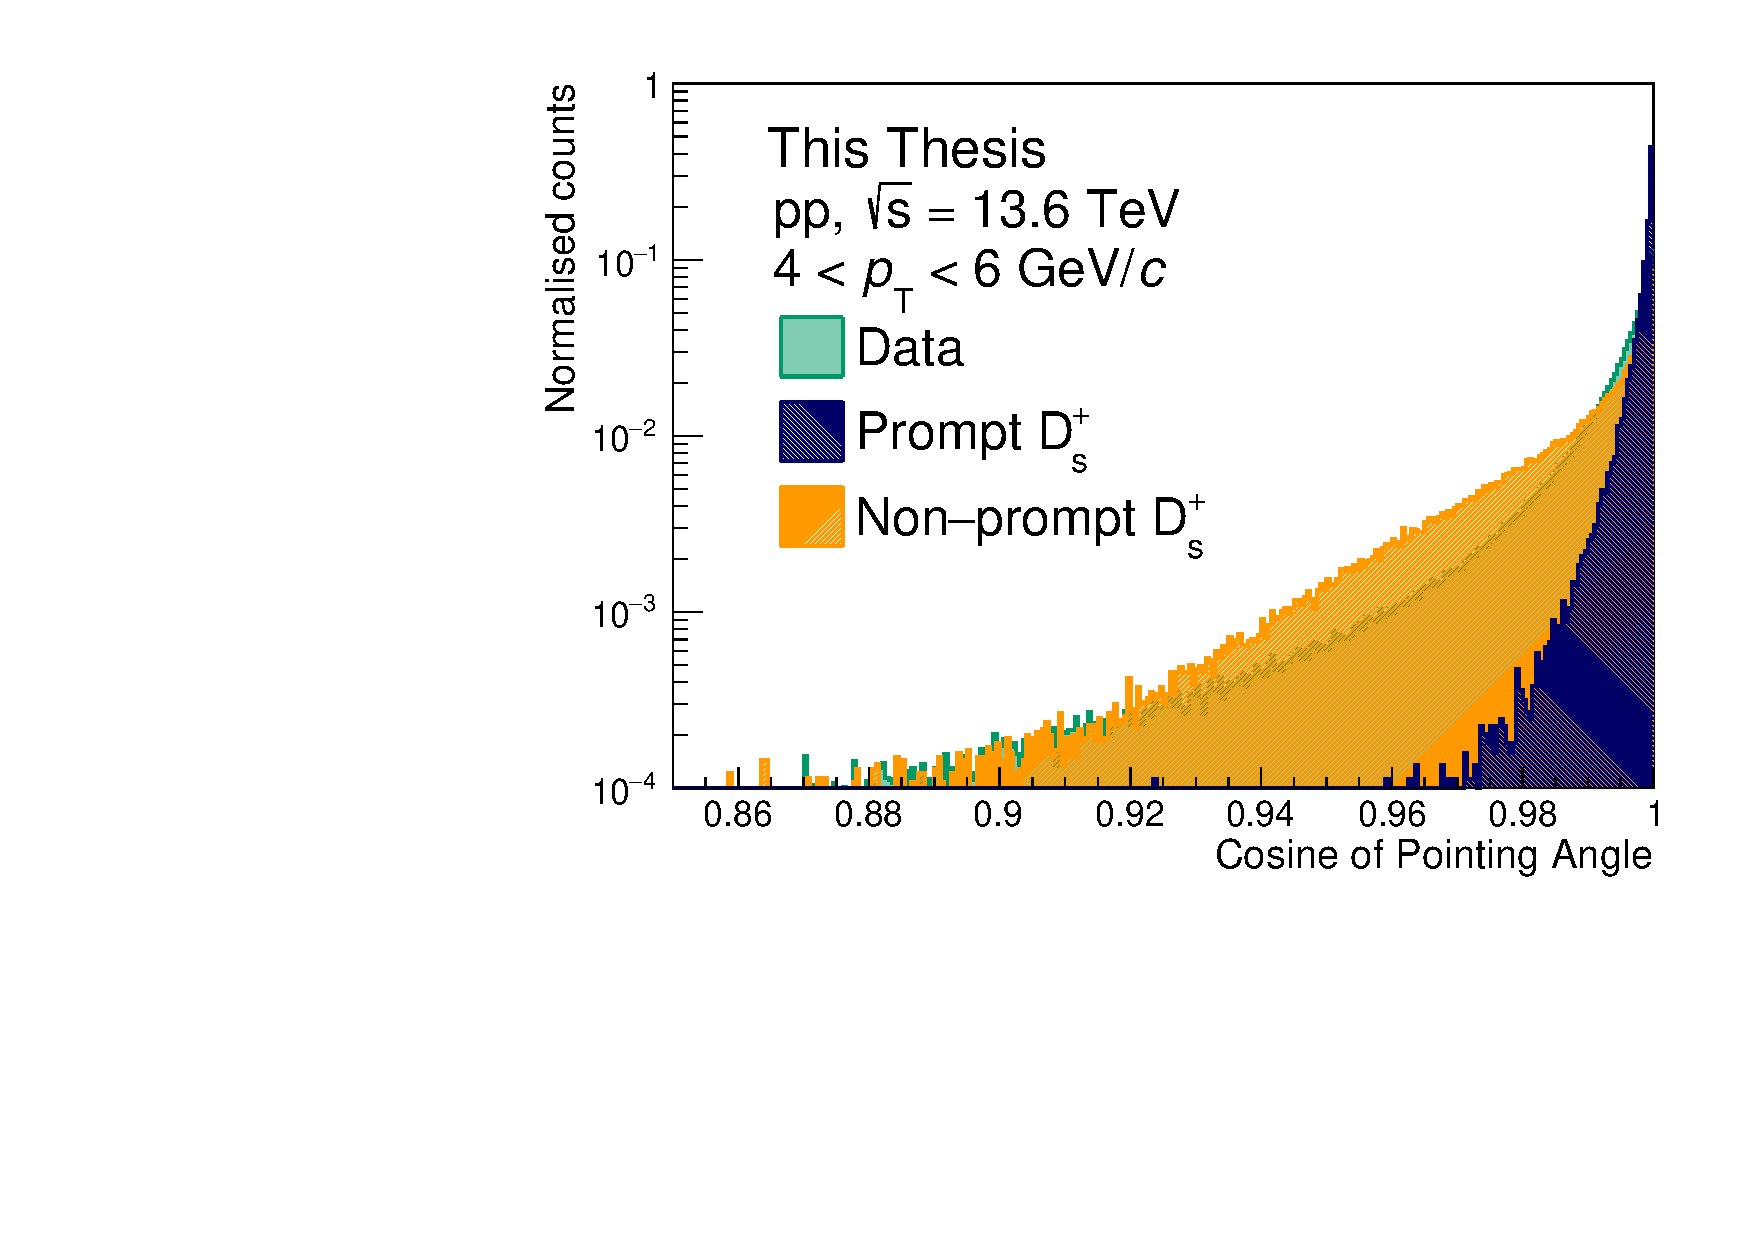
\includegraphics[width=0.48\linewidth]{Figures/Chapter 4/Cpa.pdf}
    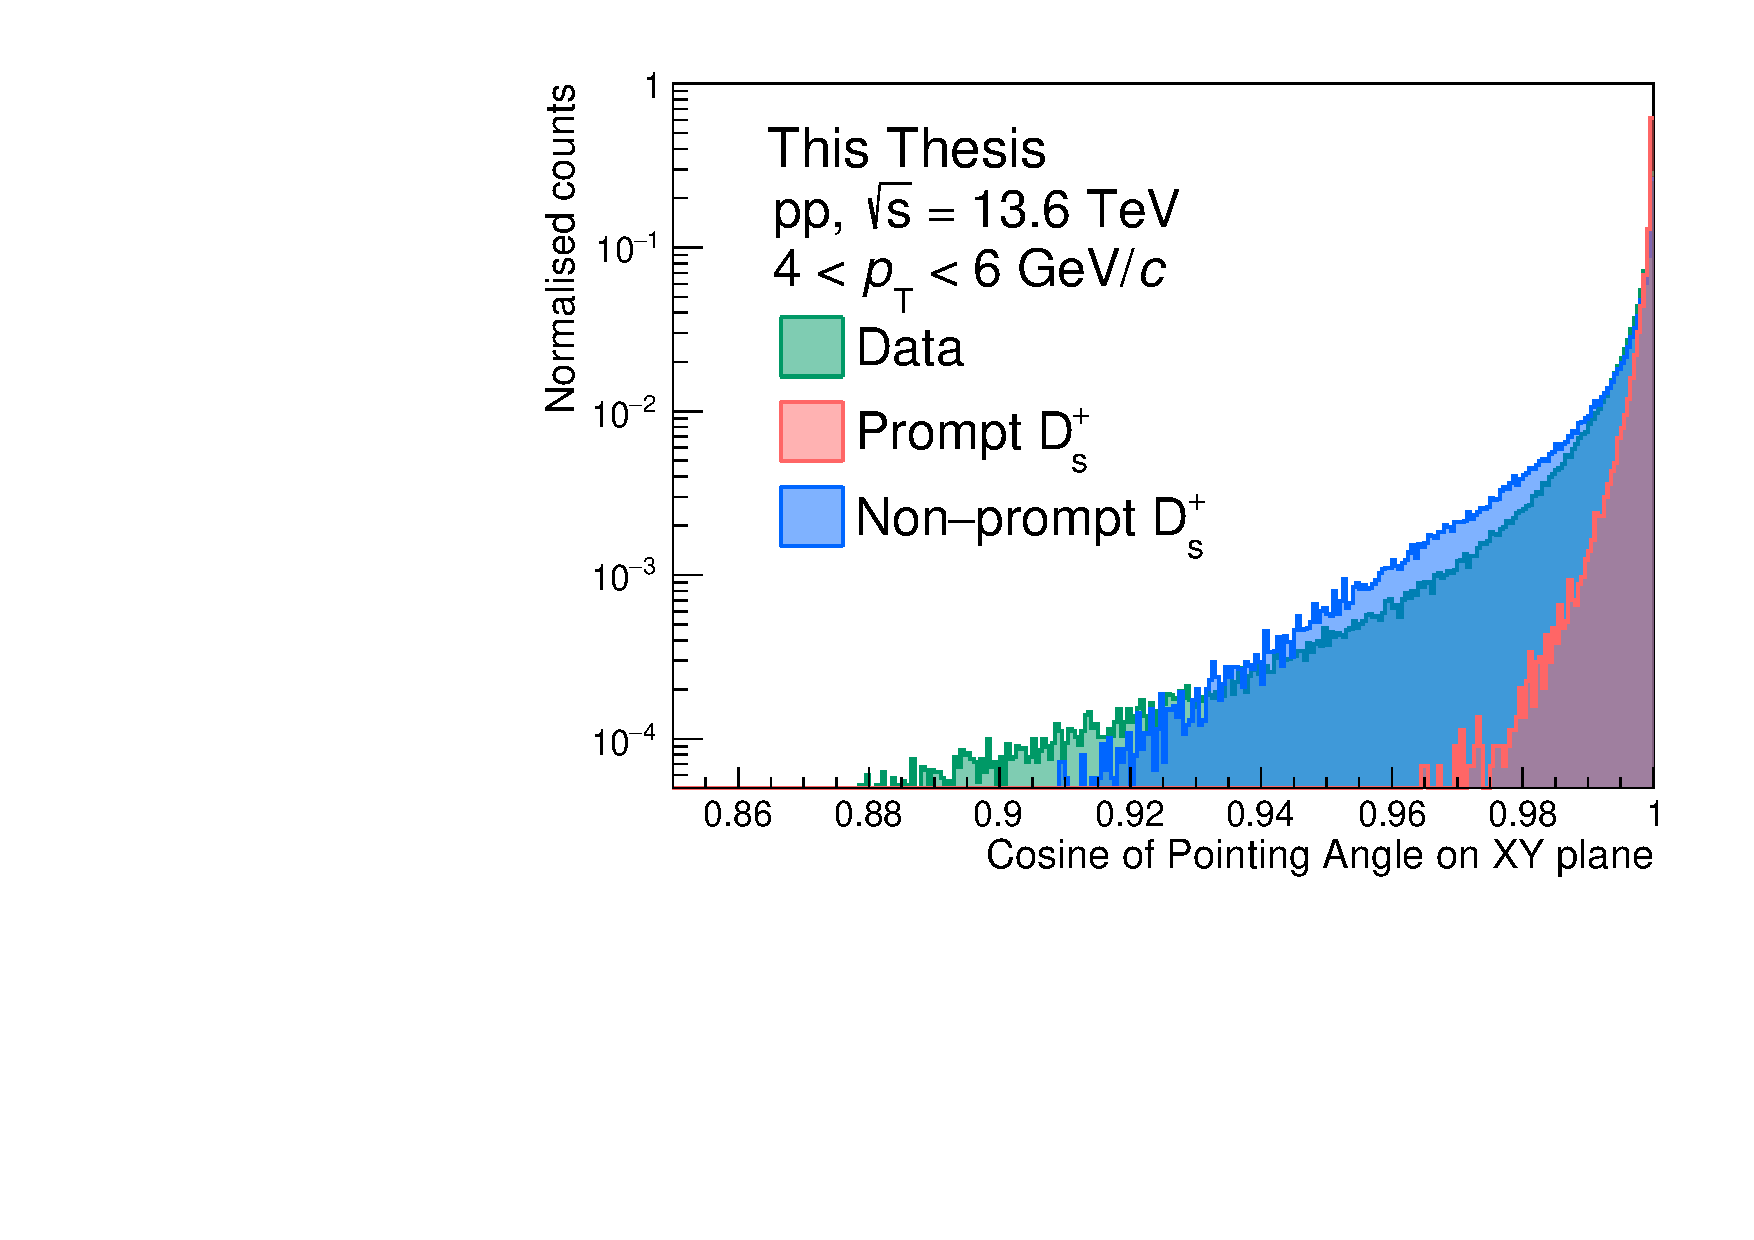
\includegraphics[width=0.48\linewidth]{Figures/Chapter 4/CpaXY.pdf}
    \caption{Distributions of the cosine of the pointing angle (left panel) and its
    projection on the transverse plane (right panel) for \ds mesons in pp collisions at \thirteen in the $4 < \pt < 6$~\gevc interval. The distributions are shown for prompt \ds mesons (blue), non-prompt \ds mesons (orange), and combinatorial background (green). For prompt and non-prompt \ds mesons, the distributions are taken from Monte Carlo simulations, whereas for combinatorial background they are taken from the data sidebands.}
    \label{fig:PointingAngle}
\end{figure}

The pointing angle $\theta_\mathrm{p}$ is defined as the angle between the flight direction of the D meson, obtained from the line connecting the primary and secondary vertices, and the direction of the reconstructed D meson momentum. This variable is also defined using only the transverse components of these quantities ($\theta_\mathrm{p}^{\mathrm{xy}}$), to exploit the better resolution in the $x$ and $y$ coordinates than in the $z$ coordinate. In an ideal scenario where particles' momentum is perfectly reconstructed, the cosine of the pointing angle for promptly-produced D mesons would be equal to 1, while that of feed-down D mesons would be distributed around 1, but with a tail towards lower values as the flight direction of the D meson is not equal to that of the parent beauty hadron. The pointing angle for the combinatorial background, on the other hand, could assume any value with the same probability. The pointing angle is therefore particularly useful to separate the signal from the combinatorial background. The distributions of the cosine of the pointing angle and its projection in the transverse plane are shown in Fig.~\ref{fig:PointingAngle} for signal and combinatorial background candidates reconstructed in the $4 < \pt < 6$~\gevc interval. Due to the finite resolution of the tracking detectors, the pointing angle is not perfectly reconstructed, leading to a distribution of the cosine of the pointing angle for prompt \ds that is peaked at 1, but with a tail towards lower values.

Similarly to the decay length, also $\theta_\mathrm{p}$ evolves with the D-meson transverse momentum. Because of the Lorentz boost, the direction of the daughter particles of the D meson is more collimated with the D-meson flight direction at higher \pt. This results in a distribution of the cosine of the pointing angle that is more peaked at 1 for higher \pt values.

\subsubsection{Impact parameter in the transverse plane}
\begin{figure}[tb]
    \centering
    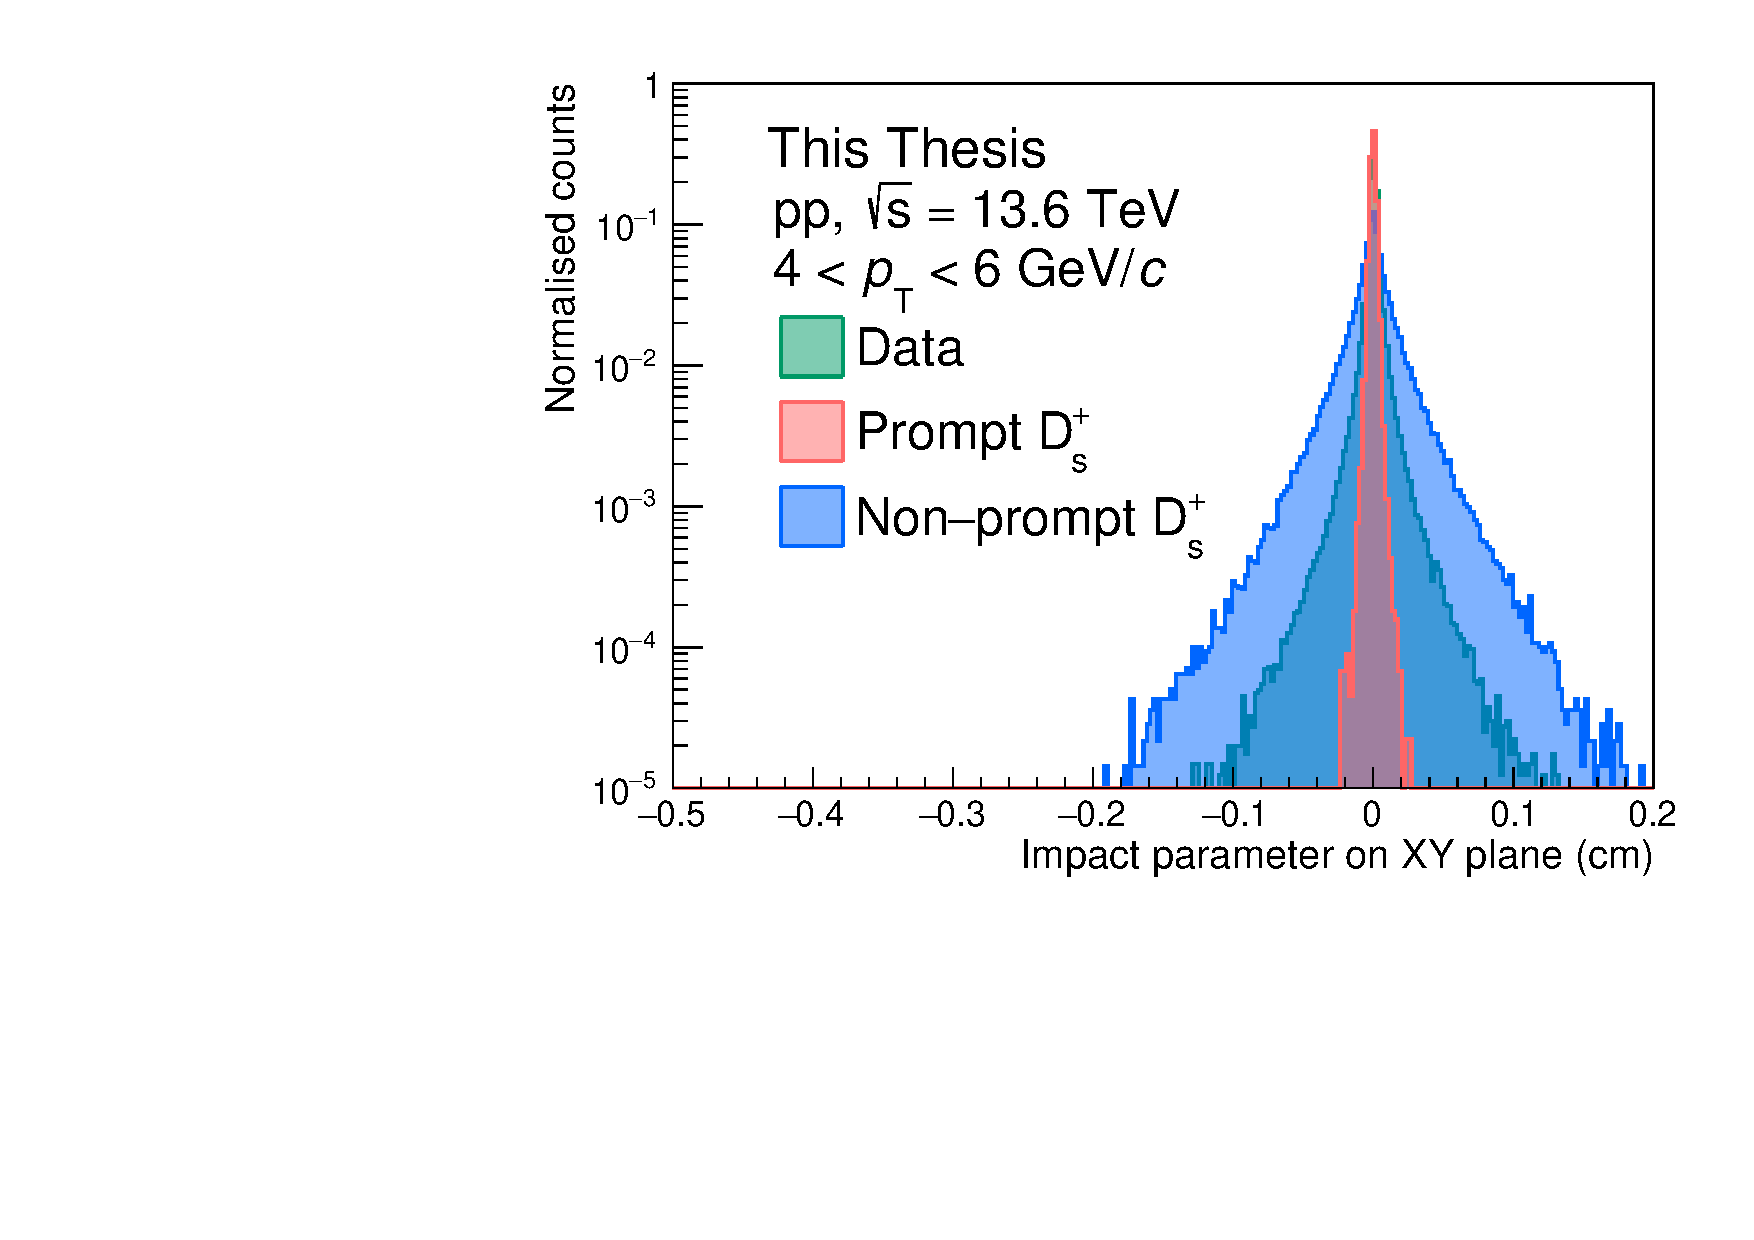
\includegraphics[width=0.48\linewidth]{Figures/Chapter 4/ImpactParameterXY.pdf}
    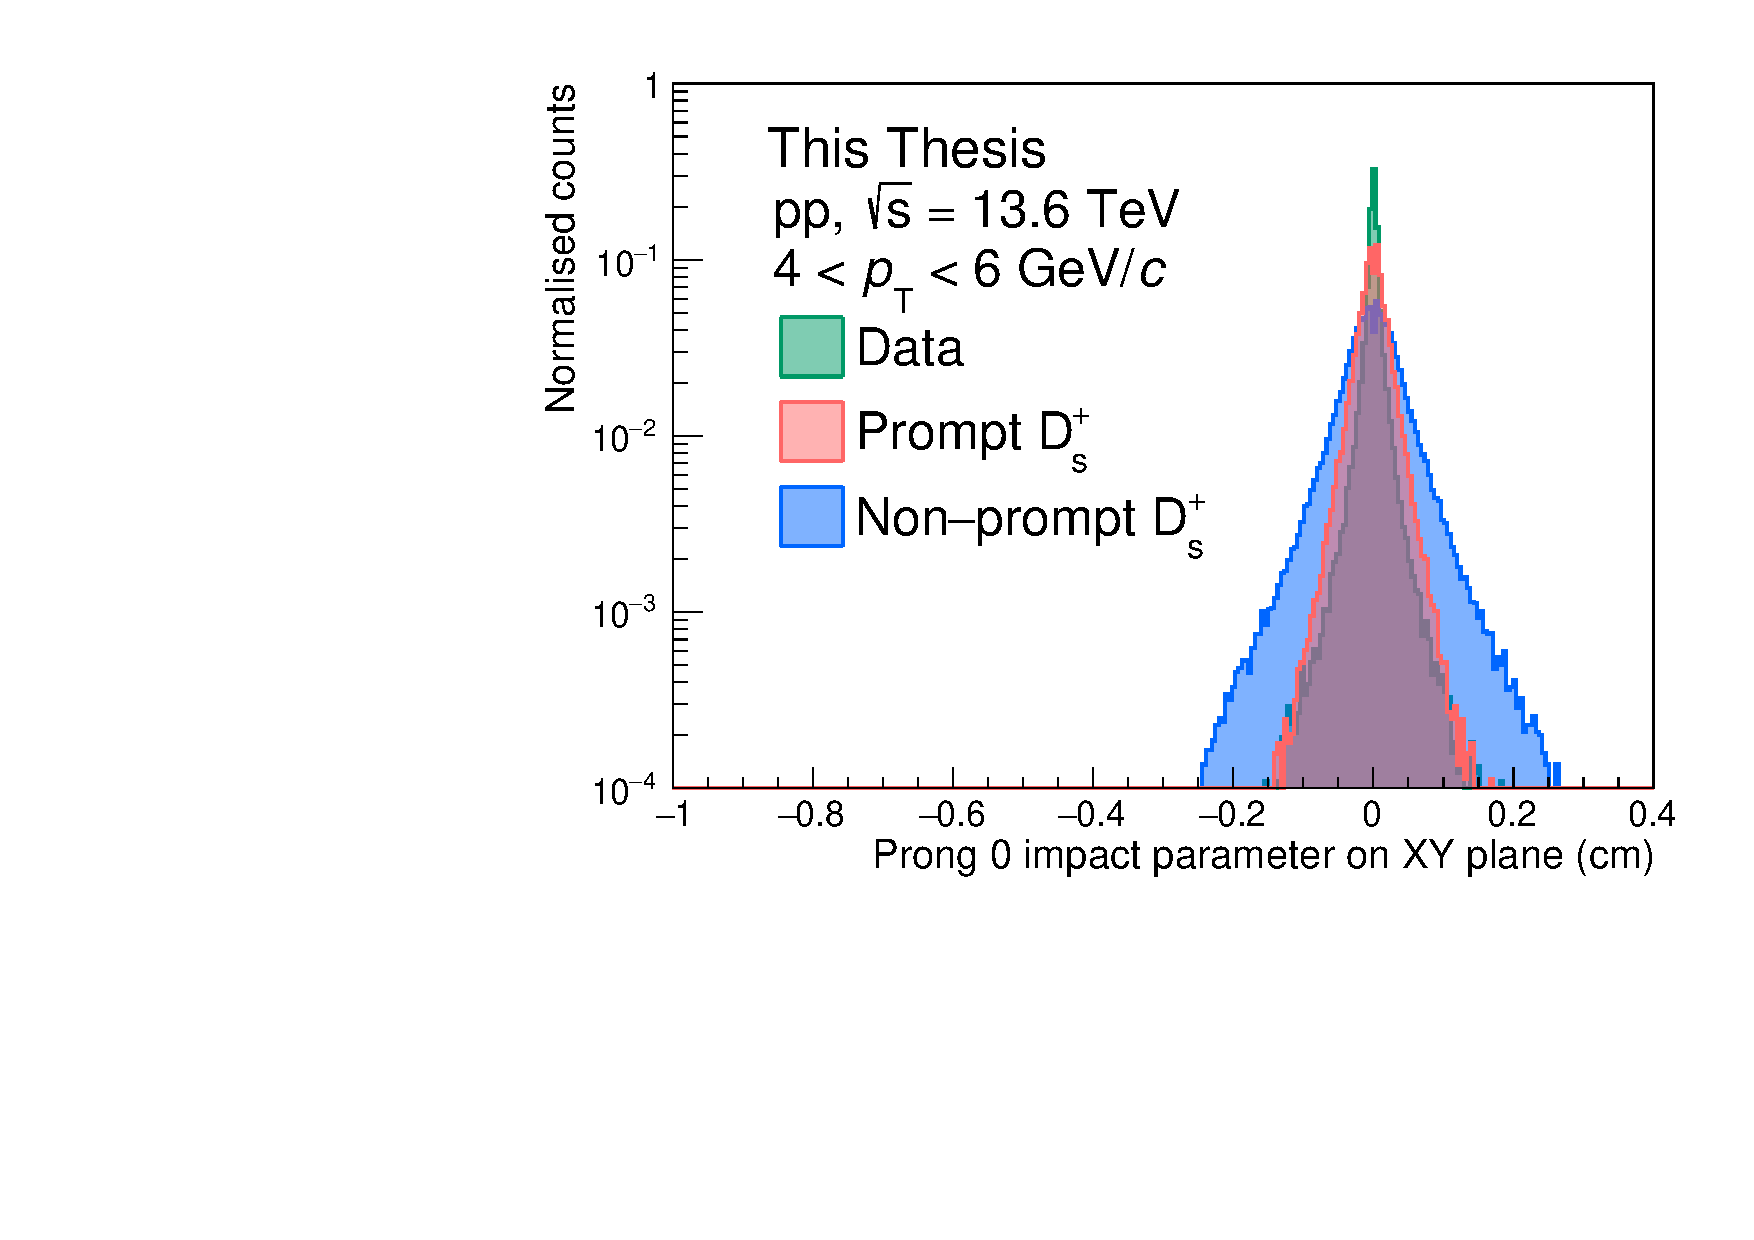
\includegraphics[width=0.48\linewidth]{Figures/Chapter 4/ImpactParameter0.pdf}
    \caption{Distributions of the projection of the impact parameter on the transverse plane for \ds mesons (left panel) and for one of the opposite-sign daughter tracks (right panel) in pp collisions at \thirteen in the $4 < \pt < 6$~\gevc interval. The distributions are shown for prompt \ds mesons (blue), non-prompt \ds mesons (orange), and combinatorial background (green). For prompt and non-prompt \ds mesons, the distributions are taken from Monte Carlo simulations, whereas for combinatorial background they are taken from the data sidebands. }
    \label{fig:ImpactParameter}
\end{figure}
The projection of the impact parameter on the transverse plane $d_0^{xy}$ is defined as the distance of closest approach between the reconstructed flight line of the D-meson and the primary vertex, projected in the $xy$ plane. It is expected to be very close to zero for promptly-produced D mesons, with any deviation due to the detector resolution. Thanks to the better momentum and vertexing resolution, its distribution becomes narrower at high \pt. It is a powerful variable not only to separate the signal from the combinatorial background, but also to discriminate between prompt and feed-down D mesons, as the latter have a much broader impact parameter distribution, as shown in the left panel of Fig~\ref{fig:ImpactParameter}. In addition, also the projection of the daughter tracks' impact parameter to the primary vertex projected on the transverse plane is used to select the signal. Since the combinatorial background does not have a secondary vertex, many of the tracks used to construct such candidates are produced directly in the primary vertex. This results in a narrow distribution of the prongs' impact parameters for such candidates. On the contrary, the displaced decay vertex of the signal candidates leads to a broader distribution of the impact parameter for prompt D-meson candidates, and to an even broader one for the non-prompt contribution to the signal, as shown in the right panel of Fig.~\ref{fig:ImpactParameter}.

\subsection{Kinematic selections}
In addition to the selections based on the decay topology, kinematic selections are also applied to increase the signal-over-background ratio and the statistical significance of the measurement.
\begin{figure}[tb]
    \centering
    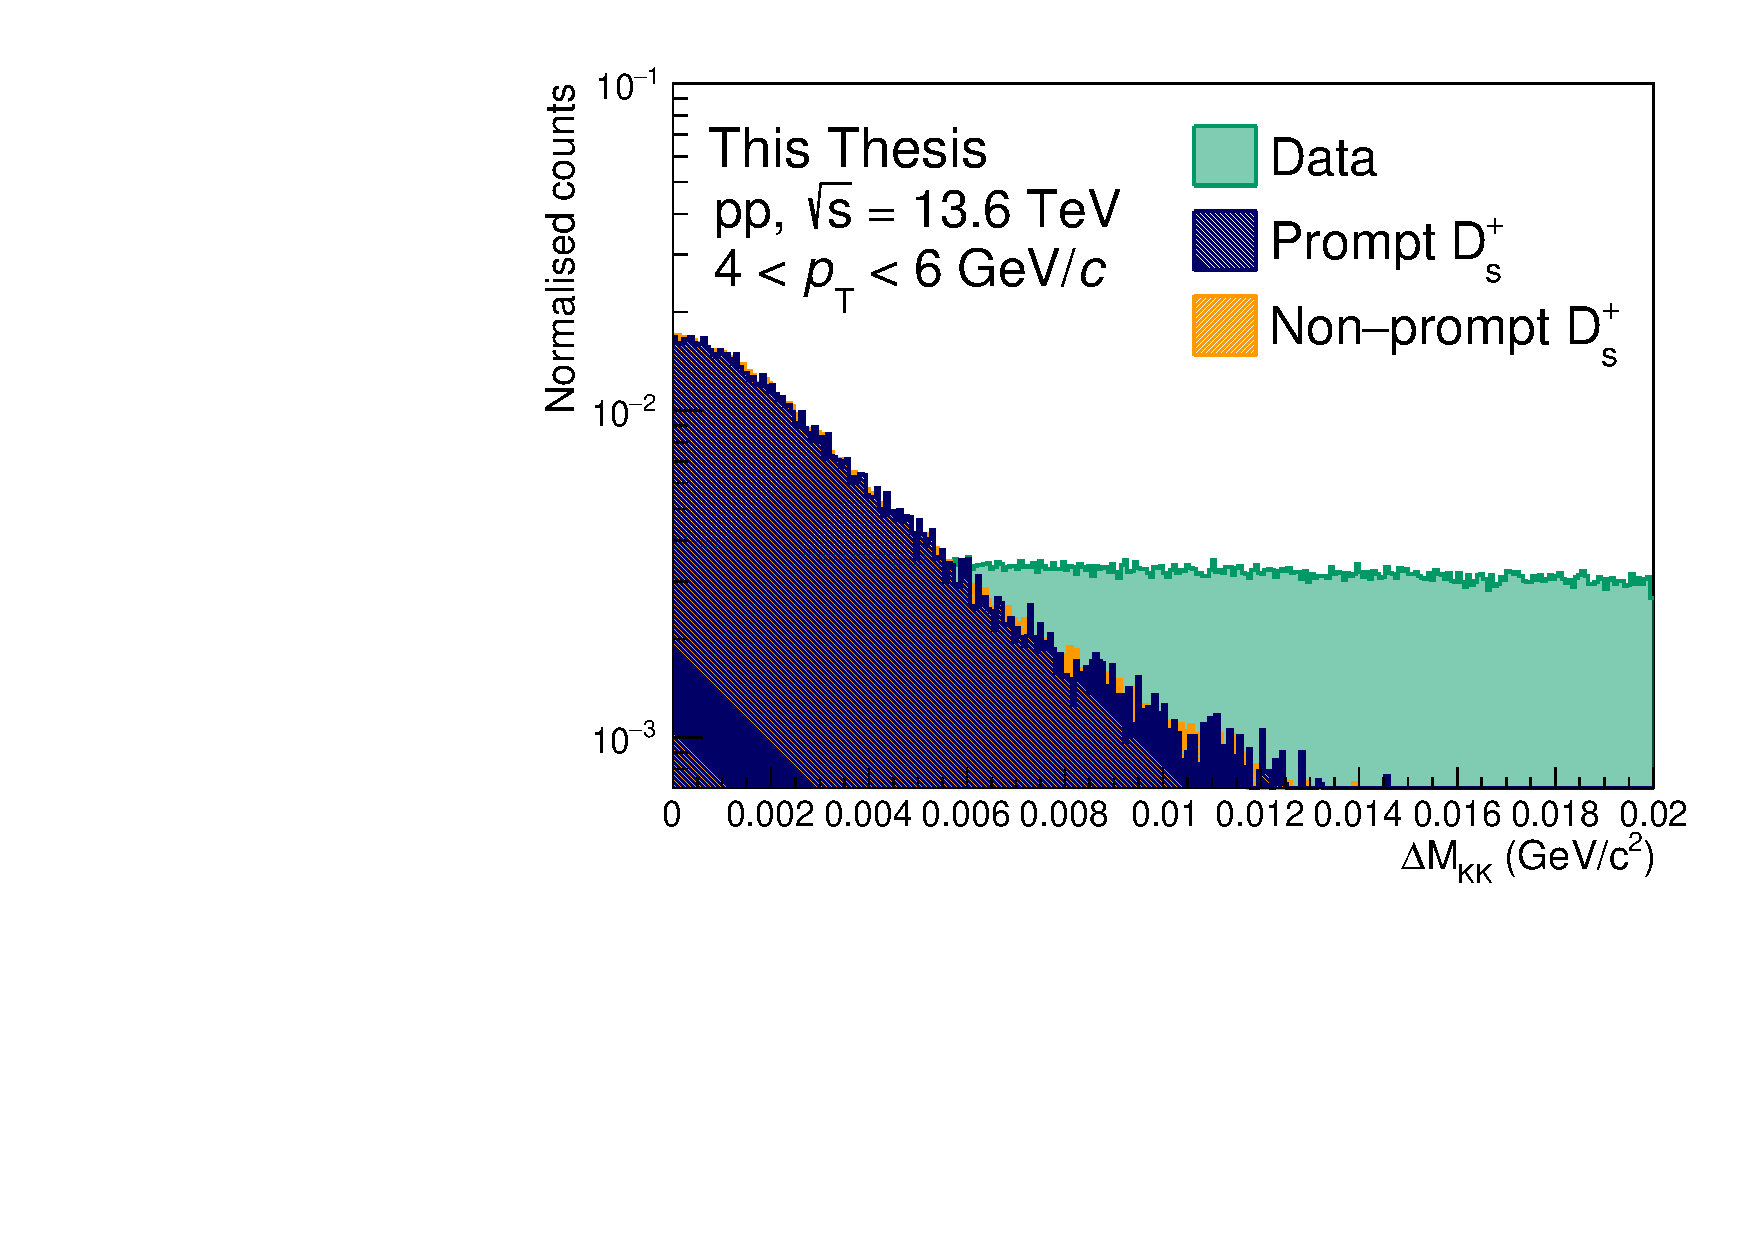
\includegraphics[width=0.48\linewidth]{Figures/Chapter 4/DeltaMassKK.pdf}
    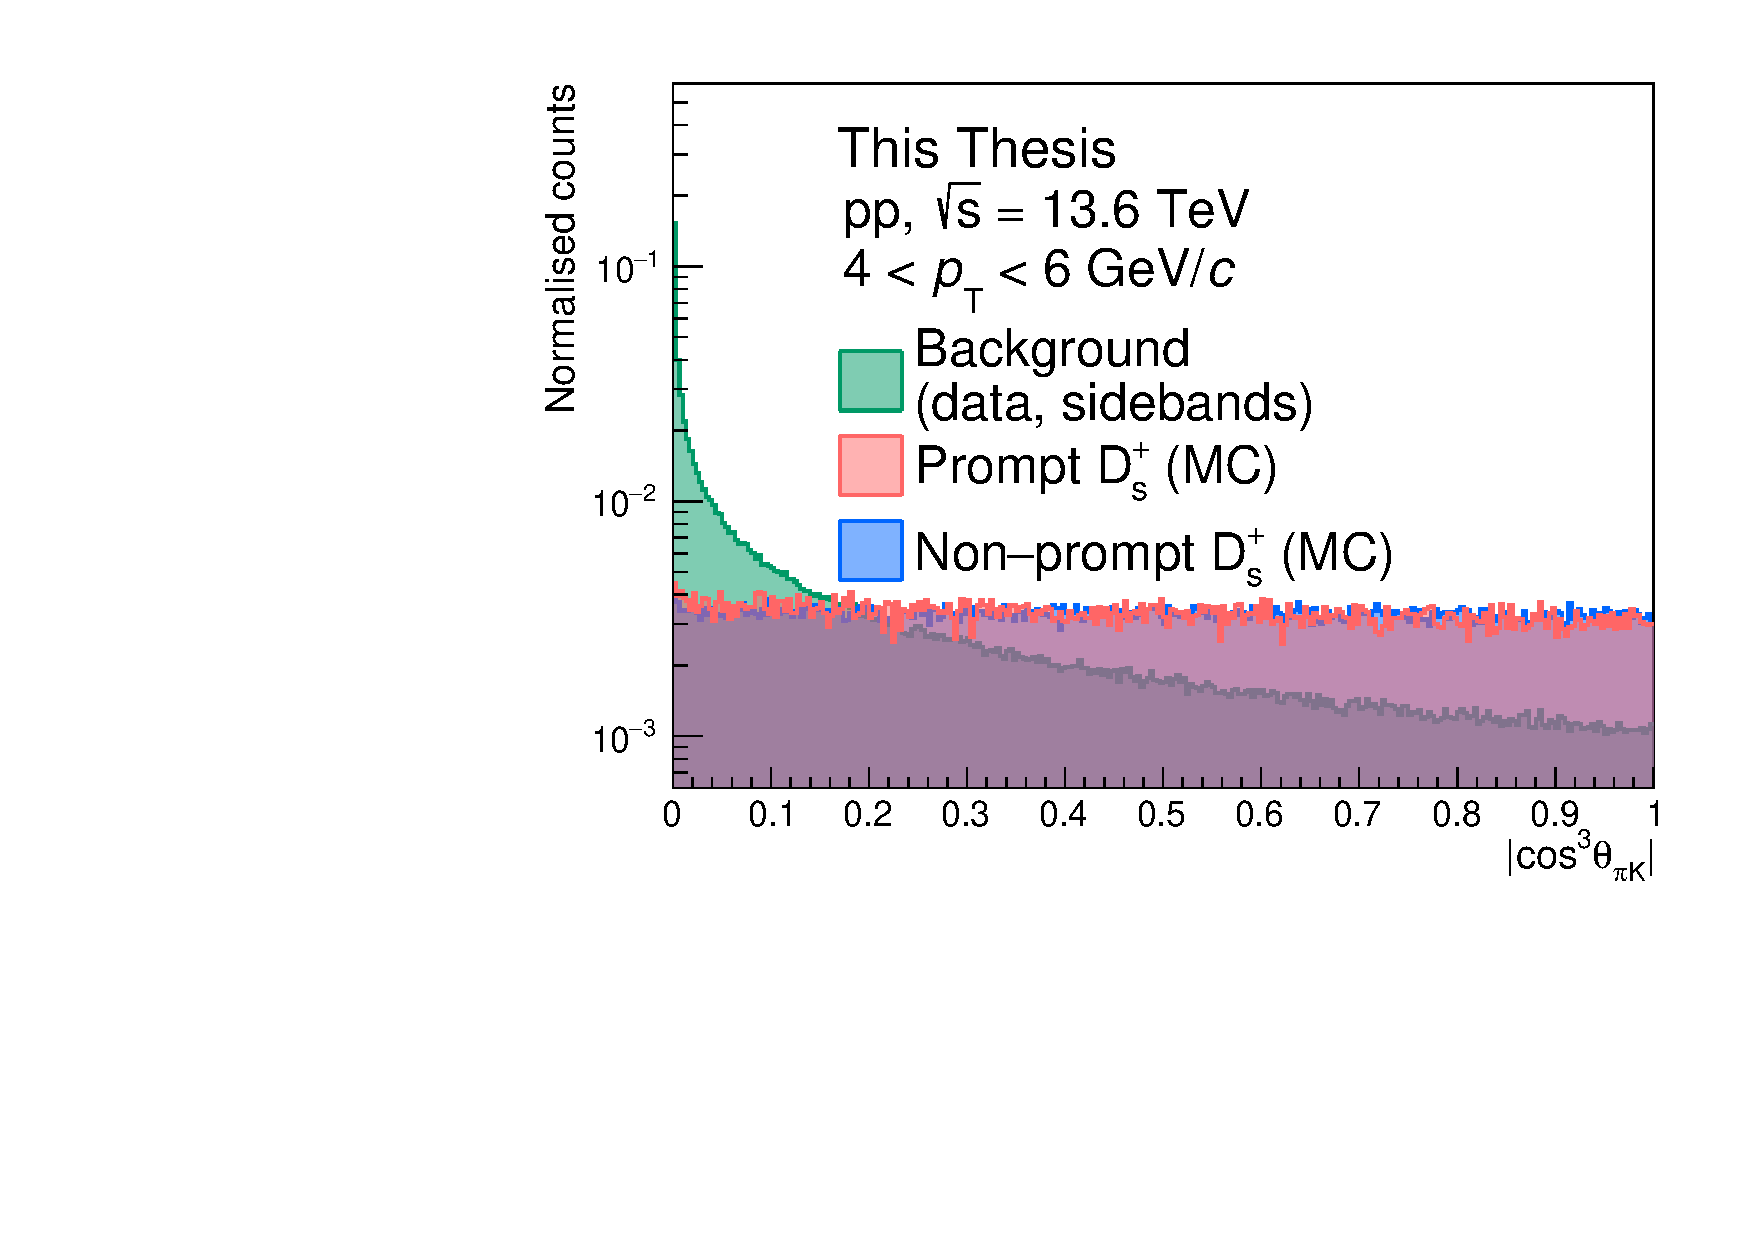
\includegraphics[width=0.48\linewidth]{Figures/Chapter 4/AbsCos3PiK.pdf}
    \caption{Distributions of the difference between the reconstructed and PDG mass of the $\phi$ meson (left panel) and the cosine cubed of the K-$\pi$ angle in the KK rest frame (right panel) for \ds mesons in pp collisions at \thirteen in the $4 < \pt < 6$~\gevc interval. The distributions are shown for prompt \ds mesons (blue), non-prompt \ds mesons (orange), and combinatorial background (green). For prompt and non-prompt \ds mesons, the distributions are taken from Monte Carlo simulations, whereas for combinatorial background they are taken from the data sidebands.}
    \label{fig:DeltaMassPhi}
\end{figure}

\subsubsection{Difference between reconstructed and PDG mass of the \boldmath$\phi$ meson}
\begin{sloppypar}
This selection exploits the production of an intermediate resonant $\phi(1020)$-meson state in the considered decay channel of the D mesons, whose invariant mass of \mbox{$M_\phi = (1019.461\pm0.016)$}~\mevcc~\cite{pdg} is well known. The $\mathrm{K^+K^-}$ pair produced in the $\phi$-meson decay is expected to have an invariant mass very close to the PDG value, as the $\phi$ resonance is narrow ($\Gamma_\phi = 4.249\pm0.013$~\mevcc~\cite{pdg}). Therefore, the difference between the reconstructed and the PDG mass of the $\phi$ meson $\lvert\Delta M(\mathrm{KK})\rvert$ is expected to be close to zero for signal candidates, while the distribution for combinatorial background is expected to be uniformly distributed.
\end{sloppypar}
Moreover, two possible $\mathrm{K^+K^-}$ pairs can be built for each triplet of tracks, depending on the mass hypothesis assigned to the like-sign tracks (e.g., for a \ds decay, both the $\mathrm{K^+K^-\pi^+}$ and $\mathrm{\pi^+K^-K^+}$ mass hypotheses can be considered). Both hypotheses are considered in the reconstruction, and the selection on $\lvert\Delta M(\mathrm{KK})\rvert$  results extremely helpful not only in rejecting the combinatorial background, but also the reflections, i.e., D mesons with the wrongly-assigned mass hypothesis.


The distribution of this variable is shown in the left panel of Fig.~\ref{fig:DeltaMassPhi} for signal and combinatorial background candidates reconstructed in the $4 < \pt < 6$~\gevc interval.

\subsubsection{Cosine cubed of the K-\boldmath$\pi$ angle in the KK rest frame}
The decay of a (pseudoscalar) D-meson to a (vector) $\phi$-meson and a (pseudoscalar) $\pi^+$ final state results in an alignment of the spin of the $\phi$ meson transverse to the direction of motion of the $\phi$ relative to the D-meson, due to elicity conservation~\cite{ATLAS:2015igt}. As a consequence, the distribution of $\mathrm{cos}\left(\theta'(\mathrm K)\right)$, where $\theta'(\mathrm K)$ is the angle between one of the kaons and the pion in the $\mathrm{K^+K^-}$
rest frame, follows a $\mathrm{cos}^2\left(\theta'(\mathrm K)\right)$ shape, which in turn implies a flat distribution for the $\mathrm{cos}^3\left(\theta'(\mathrm K)\right)$ variable, in case of signal. In contrast, the combinatorial background has a flat distribution for $\mathrm{cos}\left(\theta'(\mathrm K)\right)$, and its $\mathrm{cos}^3\left(\theta'(\mathrm K)\right)$ distribution peaks at zero. This variable is particularly useful to separate the signal from the combinatorial background, as shown in the right panel of Fig.~\ref{fig:DeltaMassPhi}.

\subsection{Particle identification selections}
One of the distinctive features of the ALICE detector are the excellent PID capabilities in a wide range of momentum, achieved by combining the information from different detectors. 

The ITS was used for its PID information during the LHC data-taking Runs~1 and 2, when the analogue readout of the SDD and SSD layers allowed for the measurement of the specific energy loss \dedx of charged particles from the charge deposited in the detector. The upgraded ITS~2 is not capable of providing such information, as the readout is now fully digital. Nonetheless, new PID techniques based on ML algorithms exploiting information such as the cluster shape and size are being developed and tested for the ITS~2. Preliminary results show that the ITS~2 PID is capable of achieving a good separation between protons and other particles, as shown in the left panel of Fig.~\ref{fig:ITSTPCPID}.

\begin{figure}[htb]
    \centering
    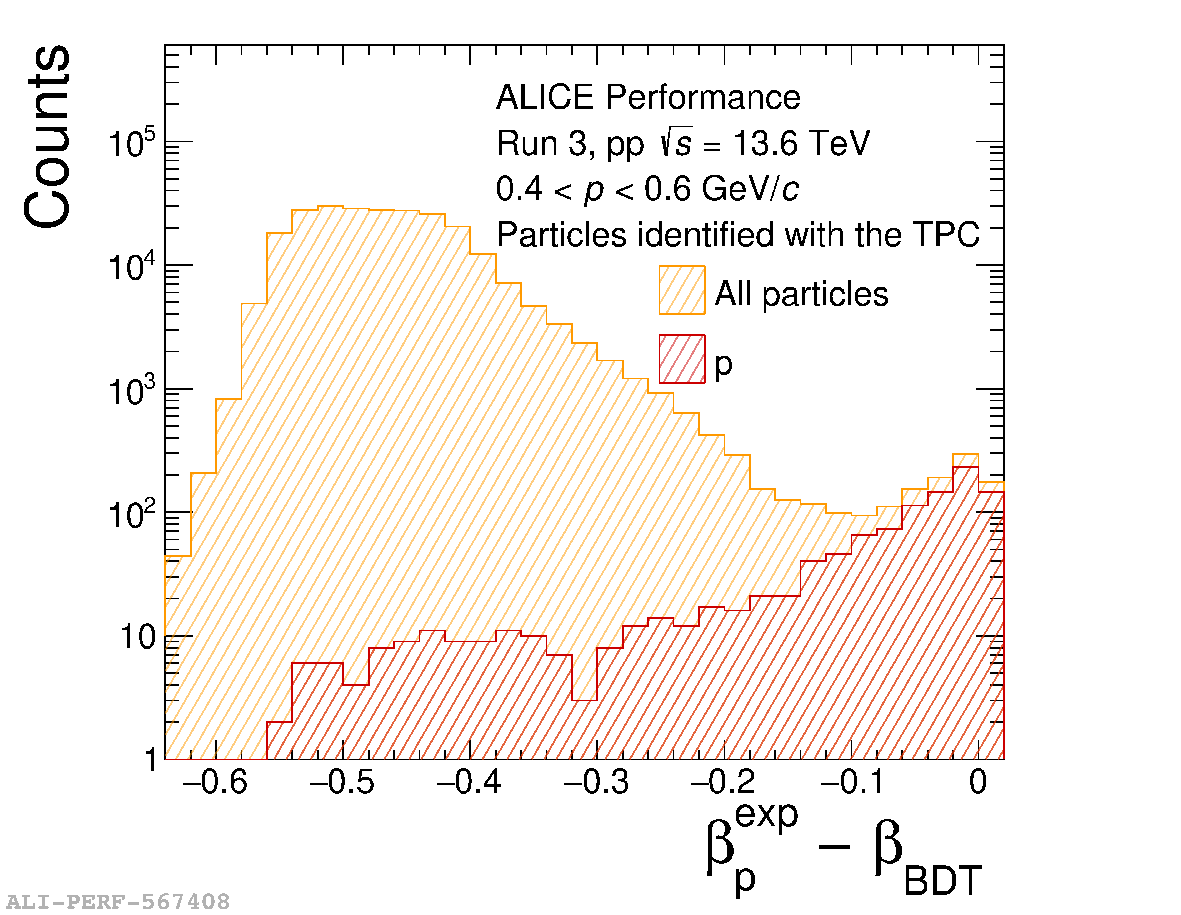
\includegraphics[width=0.48\linewidth]{Figures/Chapter 4/deltabetap-tpctagged.pdf}
    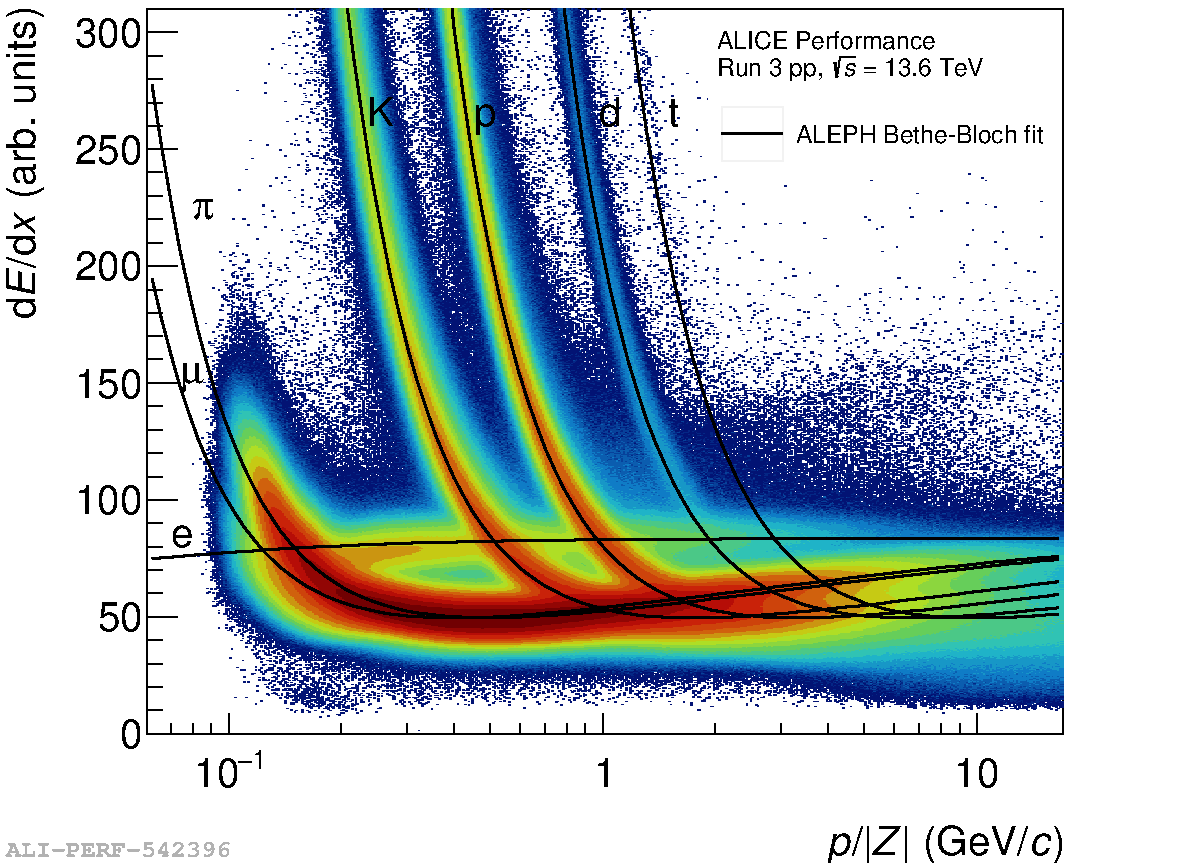
\includegraphics[width=0.48\linewidth]{Figures/Chapter 4/tpcdedx_1.pdf}
    \caption{Left: ITS 2 particle identification performance in pp collisions at \mbox{\thirteen} using a Boosted Decision Tree (BDT) regressor. From the cluster size, the regressor predicts the velocity $\beta$ ($\beta_\mathrm{BDT}$) of particles. The regressor performance is evaluated for $0.4 < p < 0.6$~\gevc, through the difference between $\beta_\mathrm{BDT}$ and $\beta\mathrm{_p^{exp}} = \frac{p}{\sqrt{p^2 + m_\mathrm{p}^2}}$. Right: Specific energy loss distribution \dedx in the TPC for pp collisions at \thirteen. The curves obtained with a fit using the ALEPH parametrisation of the Bethe-Bloch formula for electrons, muons, pions, kaons, protons, deuterium and tritium are also shown. Figures taken from the ALICE figure repository~\cite{ALICE_figures}.}
    \label{fig:ITSTPCPID}
\end{figure}

The TPC is the main PID detector in the ALICE experiment, as it provides a simultaneous measure of the specific energy loss via the charge produced in the drift voume and deposited in its 159 pad rows, the charge, and the momentum of each particle traversing the detector gas. A truncated mean of the \dedx samples is calculated discarding the 40\% highest-charge clusters, which ensures the removal of the Landau tail of the \dedx distribution caused by $\delta$-rays, which are produced from the ionisation of the gas by the electrons produced in the primary ionisation. The particle identification is based on the comparison of the measured \dedx with the expectation for a specific particle species with a certain momentum $p$. The expected \dedx is described by the Bethe-Bloch formula, and is typically parametrised with a function originally proposed by the ALEPH collaboration~\cite{Blum:2008nqe}:
\begin{equation*}
    f(\beta\gamma) = \frac{P_1}{\beta^{P_4}}\left[P_2 - \beta^{P_4} - \log\left(P_3 + \frac{1}{(\beta\gamma)^{P_5}}\right)\right]\quad .
\end{equation*}
In this parametrisation, $\beta$ and $\gamma$ are the particle velocity and Lorentz factor, respectively, and $P_{1-5}$ are the parameters of the fit function. The \dedx distribution in the TPC is shown in the right panel of Fig.~\ref{fig:ITSTPCPID} for pp collisions at \thirteen. The curves obtained with a fit using the ALEPH parametrisation of the Bethe-Bloch formula for electrons, muons, pions, kaons, protons, deuterium and tritium are also shown. While in the non-relativistic low momentum region ($p \leq 1$~\gevc) p, K and $\mathrm{\pi}$ can be separated on a track-by-track basis, at higher momenta, in the relativistic rise region, particles can still be identified on a statistical basis via multi-Gaussian fits. This is possible because the truncated-mean method produces a \dedx peak with a gaussian shape down to three orders of magnitude for long tracks (at least 130 clusters)~\cite{ALICE:2014sbx}.

The TOF detector is dedicated to PID in the intermediate momentum range, up to 2.5~\gevc for pions and kaons, and up to 4~\gevc for protons. In this region, the TPC is not able to provide a sufficient separation between the different particle species. The TOF detector is based on the measurement of the time of flight of charged particles between the interaction point and the detector. The start time is provided by the FT0 forward-rapidity detectors, and a total time resolution of the 80~ps is achieved, allowing for a separation of the different particle species based on the time of flight. The TOF PID performance is shown in Fig.~\ref{fig:TOFPID} for \pbpb collisions at $\sqrt{s_\mathrm{NN}} = 5.02$~\tev. The large background is due to tracks that are incorrectly matched to TOF hits in high-multiplicity \pbpb collisions.

\begin{figure}
    \centering
    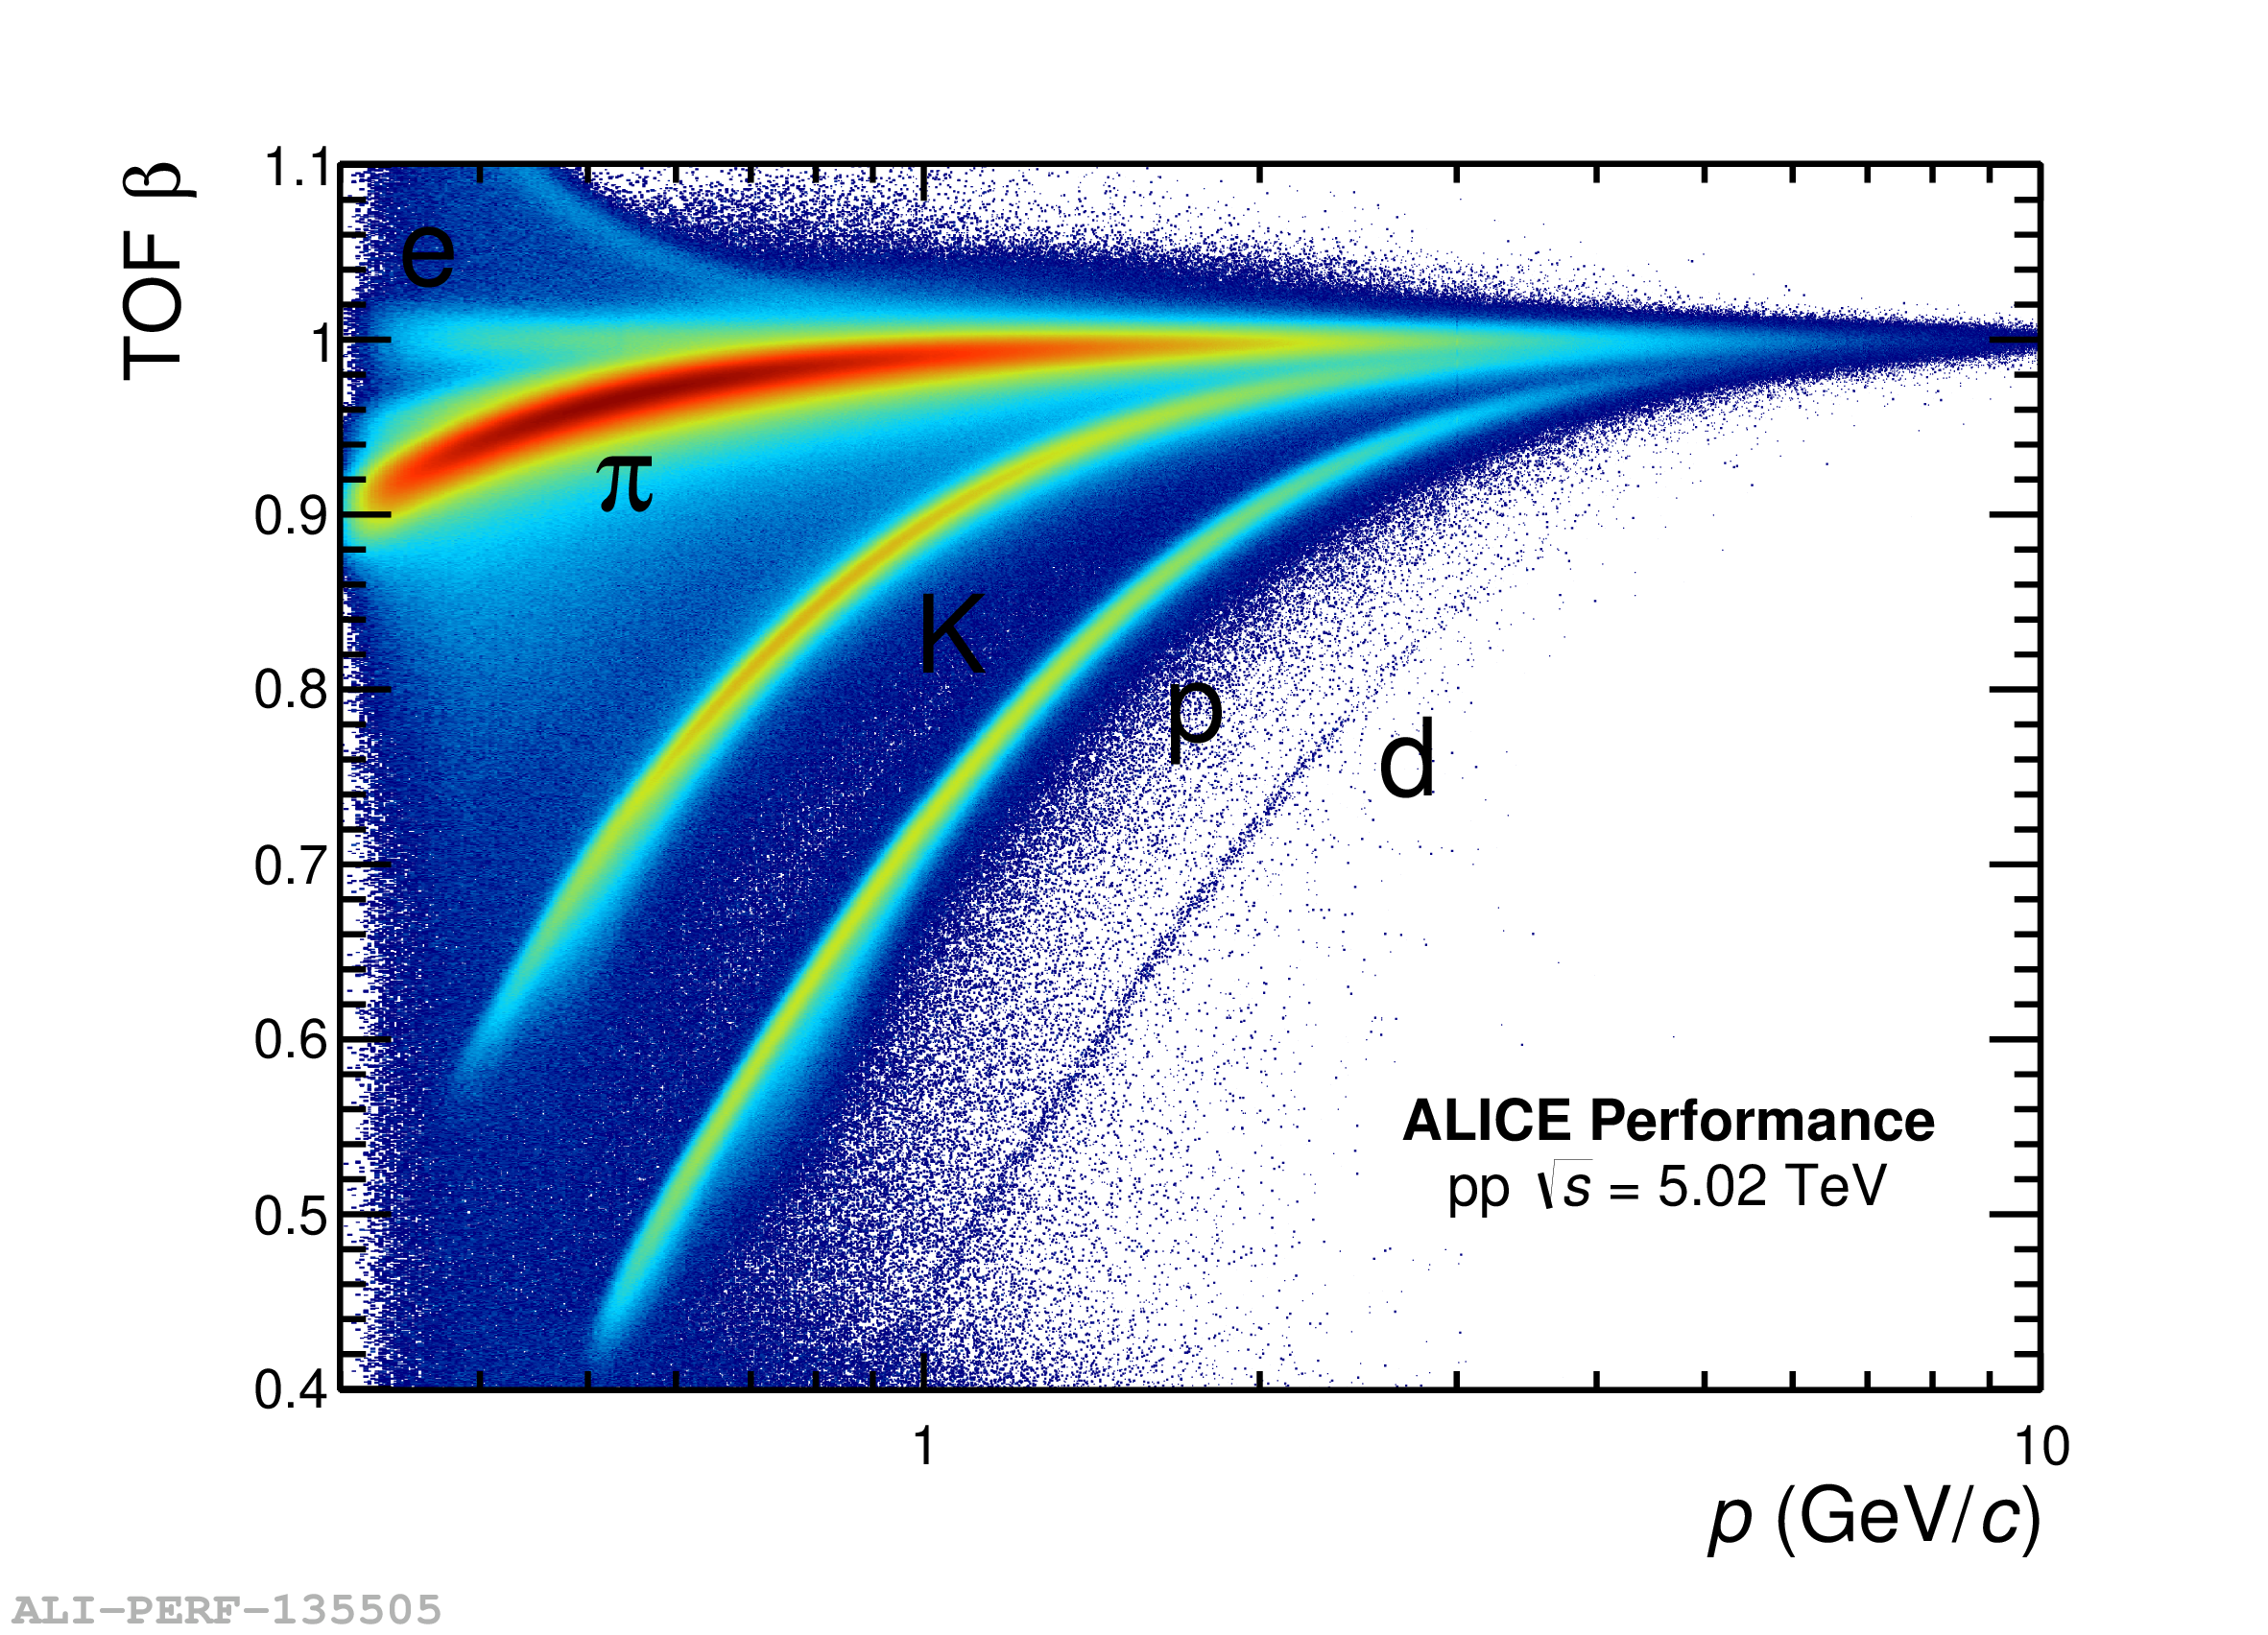
\includegraphics[width=0.7\linewidth]{Figures/Chapter 4/TOFBeta_pp.png}
    \caption{$\beta$ parameter measured with the TOF detector as a function of the momentum $p$ measured by the TPC detector in \pbpb collisions at $\sqrt{s_\mathrm{NN}} = 5.02$~\tev. Figure taken from the ALICE figure repository~\cite{ALICE_figures}.}
    \label{fig:TOFPID}
\end{figure}

Other detectors, such as the High Momentum Particle Identification Detector (HMPID) or the Transition Radiation Detector (TRD), complement the PID capabilities of the ALICE experiment. The HMPID is dedicated to the identification of particles with momenta above 2~\gevc, and is based on the detection of Cherenkov radiation emitted by charged particles traversing a radiator. The TRD is used for the identification of electrons and positrons, and is based on the detection of transition radiation emitted by charged particles traversing a radiator with a change in the dielectric constant. The TRD is particularly useful for the identification of electrons and positrons in the high-multiplicity environment of heavy-ion collisions, where the TPC and TOF detectors are not able to provide a sufficient separation between electrons and pions. 

The PID infromation on the decay tracks can be exploited to improve the background rejection and thereby the signal extraction. For this analysis, only the inforamation from the TPC and TOF detector is used, as the ITS PID capabilities are still under development, and the final state particles of the D mesons are pions and kaons, which can be well identified with the TPC and TOF detectors. A track is considered compatible with a mass hypothesis (i.e. a hadron species) depending on the difference between the measured signal $S_\mathrm{meas}^\mathrm{TPC,TOF}$ and the expected signal $S_\mathrm{exp (\pi, K, p)}^\mathrm{TPC,TOF}$ for the given hypothesis. The measured signal is the truncated mean of the \dedx distribution for the TPC detecotr, and the time of flight for the TOF detector. The expected signal is extracted from the ALEPH parametrisation of the Bethe-Bloch formula described above for the TPC, and from a parametrisation of the distribution of $\beta$ as a function of $p$ for the TOF. The difference between the measured and expected signals is then usually normalised by the uncertainty on the measured signal $\sigma_\mathrm{TPC, TOF}$:
\begin{equation*}
    \mathrm{n}\sigma_\mathrm{\pi, K, p}^\mathrm{TPC, TOF} = \frac{\lvert S_\mathrm{meas}^\mathrm{TPC, TOF} - S_\mathrm{exp (\pi, K, p)}^\mathrm{TPC, TOF}\rvert}{\sigma_\mathrm{TPC, TOF}}\quad .
\end{equation*}
Tracks are considered if at least one PID signal is available from one of the two detectors. A loose preselection is applied to the candidates based on PID information, requiring the three tracks to have a $\mathrm{n}\sigma^\mathrm{TPC} < 5$, or $\mathrm{n}\sigma^\mathrm{TOF} < 5$ for the considered mass hypothesis. This selection effectively reduces the amount of reflections in the data sample, as the wrongly-assigned mass hypothesis are often rejected.

Due to a TPC--TOF matching efficiency which is significantly lower than unity, the PID information from the two detectors is typically combined to obtain a single PID variable $\mathrm{n}\sigma^\mathrm{comb}_\mathrm{\pi, K, p}$, which is used in the final selection. The PID information is combined as
\begin{equation*}
    \mathrm{n}\sigma^\mathrm{comb}_\mathrm{\pi, K, p} = 
    \begin{cases}
        \mathrm{n}\sigma^\mathrm{TOF}_\mathrm{\pi, K, p} & \text{only TOF information is available}\\
        \mathrm{n}\sigma^\mathrm{TPC}_\mathrm{\pi, K, p} & \text{only TPC information is available}\\
        \frac{1}{\sqrt{2}}\sqrt{(\mathrm{n}\sigma^\mathrm{TPC}_\mathrm{\pi, K, p})^2 + (\mathrm{n}\sigma^\mathrm{TOF}_\mathrm{\pi, K, p})^2} & \text{otherwise}\\
    \end{cases}
\end{equation*}
This reduces the number of features used for the Machine Learning analysis described in the following Chapters, and ensures a proper handling of sparse data.



\setcounter{chapter}{4}
%\chapter{\texorpdfstring{\ds and \dpl signal extraction}{Ds+ and D+ signal extraction}}\label{chap:RY}

The main ingredient for the evaluation of the \ds/\dpl production-yield ratio are the \ds- and \dpl-meson raw yields, i.e., the number of reconstructed and selected \ds and \dpl mesons. Due to the vast amount of combinatorial background, the extraction of the raw yields through a simple candidate counting method is not feasible. Instead, the raw yield is obtained on a statistical basis by fitting the invariant-mass distribution of the \ds- and \dpl-meson candidates passing tight selection criteria. To reduce the combinatorial background and preserve the highest possible efficiency of D-meson selection, Machine Learning algorithms have been employed. The following sections describe the procedure for the extraction of the raw yield of \ds and \dpl mesons. 


\section{Machine Learning}
The term \emph{Machine Learning} (ML) is a broad and versatile concept, encompassing a wide range of algorithms that grant computers the capacity to learn and adapt without being explicitly programmed to do so~\cite{5392560}. A more comprehensive definition characterises ML as the study of algorithms that enhance their performance at a specific task through the accumulation of experience~\cite{mitchell1997machine}. In recent years, ML techniques have witnessed widespread adoption across diverse fields, with significant impacts realised especially with the emergence of generative models such as GPT~\cite{openai2023gpt4}. ML algorithms have found extensive applications in the high-energy physics field, primarily for the task of distinguishing interesting signals from the vast background present in particle-collision data. Furthermore, these algorithms have been employed as triggers, aiding in the rapid identification of events of interest, and have also been instrumental in event reconstruction. Notably, ML algorithms were used in the discovery of the Higgs boson~\cite{CMS:2012qbp}, one of the most significant achievements in the field of particle physics of the last decades.



\subsection{Supervised learning}
Supervised learning is one of the main branches of machine learning, along with unsupervised and reinforcement learning. Machine learning tasks are usually described in terms of how the machine learning system should process an example, which is a collection of features $\mathbf{x}$ that have been quantitatively measured from some object or event that one wants the machine learning system to process. In the case of supervised learning, each example is coupled with a corresponding label or target, $\mathbf{y}$. The objective of supervised learning is to learn to predict or infer $\mathbf{y}$ based on the associated features, $\mathbf{x}$, assuming that there exists a functional relationship $\mathbf{y} = f(\mathbf{x})$ between the two. The goal of the ML system is to produce an approximation $\widehat{f}(\mathbf{x})$ of the true function $f(\mathbf{x})$ by minimising a given loss function, which quantifies the discrepancy between the predicted and true labels. Supervised learning problems are further segmented into two distinct sub-categories: classification and regression. In the former, the label $\mathbf{y}$ assumes values from a finite and discrete set of categories, often representing distinct classes or groups. In the latter, the label $\mathbf{y}$ takes the form of one or more continuous variables, necessitating the learning system to deduce a continuous function or mapping between $\mathbf{x}$ and $\mathbf{y}$.

The usage of ML algorithms in classification problems, such as the one presented in this Thesis, allows for the definition of multi-dimensional non-linear decision boundaries, which are not available with traditional selection methods based on linear selections on some cut variables. This is particularly important as it provides more efficient selections and a larger purity of the selected data sample.

The application of a supervised learning algorithm to a dataset involves the following steps: i) the model's hyperparameters are optimised through reduced training phases; ii) the optimised model is trained on a set of labelled data, i.e., the value of $\mathbf{y}$ is known for each example in the training set; iii) the model is tested on a separate set of labelled data, known as the test set, to evaluate its performance; iv) the model is then used to make predictions on new, unseen data.

\subsubsection{Hyperparameters tuning}
Before the training phase, hyperparameter tuning is performed to optimise the model's performance. \emph{Hyperparameters} are parameters that are not learned during the training process, but rather define the model's architecture and the training process itself. Hyperparameter tuning is usually performed through a grid search, random search, or with a more efficient bayesian optimisation~\cite{frazier2018tutorial,snoek2012practical,mockus2005bayesian}. Several combinations of hyperparameters are tested on a dedicated labelled dataset: the validation set. Models with different hyperparameter sets are trained with a reduced training phase, and the one yielding the best performance is then selected for a full training phase.

\subsubsection{Training}
During the training process, the model learns (i.e., adjusts its internal parameters) to map the input features $\mathbf{x}$ to the corresponding labels $\mathbf{y}$ by minimizing a given loss function. Typically used loss functions include the Mean Squared Error (MSE) for regression tasks and the Cross-Entropy loss~\cite{mao2023cross} for classification tasks. The loss function is minimised through an optimisation algorithm, usually stochastic gradient descent~\cite{10.1214/aoms/1177729392}, which iteratively updates the model parameters to reduce the loss. Since an over-optimisation of the model on the training data can lead to poor generalisation on unseen data (the model is said to be \emph{overfitting}), a regularisation term is often added to the loss function to penalise overly complex models. The training process continues until the model reaches a satisfactory level of performance on the training data, or until its performance does not improve further. 

\subsubsection{Cross-validation}

With the strategy defined above to optimise the hyperparameters and train the model, the training dataset is divided into two subsets: the validation set and the training set, which are used for hyperparameter tuning and training, respectively. When small datasets are involved, this division can lead to a suboptimal model, as the model's performance can be highly dependent on the specific examples in the training and validation sets. Furthermore, this approach limits the amount of data available for training the model, which can lead to poor generalisation. To mitigate this issue, cross-validation~\cite{stone1974cross} is often employed. This term refers to a set of techniques that allow for a more robust estimate of the model's generalisation performance by using the entire dataset for training and validation. The most common cross-validation technique is the $k$-fold cross-validation. It consists in dividing the training sample into $k$ subsets of equal size, called \emph{folds}. Then, the ML algorithm is trained $k$ times, each time using $k-1$ folds as training set, while the remaining fold is used as validation set. The model's performance is then averaged over the $k$ folds to obtain a more robust estimate of this quantity. This operation is repeated for each hyperparameter configuration to be considered. The hyperparameter configuration minimising the loss function or other metrics used to evaluate the model's performance is then chosen as the optimal configuration.


\subsubsection{Testing}
After the model has been trained, its performance is evaluated on a dataset that was not used during the training process, known as the test set. Like the training and validation sets, also the test set contains labelled examples, but the labels are not provided to the model. While the model is optimised to minimise the loss function during the training phase, the test set is used to estimate the model's generalisation error, i.e., how well the model performs on unseen data. The model's performance is evaluated using metrics that are specific to the task at hand, such as accuracy for classification tasks, or Mean Squared Error (MSE) for regression tasks. Once the model achieves satisfactory performance on the test set, it is ready to be used for making predictions on unlabelled data.


\section{\texorpdfstring{\ds and \dpl selection using Machine Learning}{Ds+ and D+ selection using Machine Learning}}

The task of extracting \ds- and \dpl-meson signals from the vast combinatorial background is a challenging one, due to the large amount of background compared to signal. It is however an excellent example of classification problem, and ML algorithms can therefore be exploited to enhance the efficiency of the selection. 

\subsection{Data preparation}\label{sec:ml_data_preparation}
In order to train a ML model, a labelled dataset with a well-defined set of features is required. The dataset used for training the ML algorithms employed in this Thesis is composed of a number of signal and background examples. To obtain a pure sample of signal candidates, Monte Carlo (MC) simulations are used to generate \ds and \dpl mesons and transport their decay products through a simulation of the ALICE apparatus. Proton-proton collisions are simulated using the \textsc{Pythia~8} event generator~\cite{Bierlich:2022pfr} with colour-reconnection Mode~2~\cite{Christiansen:2015yqa}, and the generated particles are propagated through the ALICE detector using the \textsc{Geant4} transport simulation toolkit~\cite{GEANT4:2002zbu}. A dataset enriched of heavy-flavour hadrons is obtained by only selecting (\emph{triggering}) events where at least a $\mathrm{c\overline{c}}$ or $\mathrm{b\overline{b}}$ pair is produced. The produced \ds and \dpl mesons are then forced to decay into the studied decay channels, i.e.: \mbox{$\ds \rightarrow \phi \pi \rightarrow \mathrm{K^+K^-\pi^+}$}, $\ds \rightarrow \mathrm{K^+K^{*0}}\rightarrow \mathrm{K^+K^-\pi^+}$, characterised by the same $\mathrm{K^+K^-\pi^+}$ final state, $\dpl \rightarrow \mathrm{\pi^+K^-\pi^+}$, and $\dpl \rightarrow \phi \pi \rightarrow \mathrm{K^+K^-\pi^+}$. 

%Due to the displaced topology of heavy-flavour decays and the continuous readout employed by the ALICE detector, the selection of events with charm or beauty hadrons produces ``fake'' vertices arising from the association of displaced decay tracks, affecting the reconstruction of heavy-flavour hadrons. To overcome this problem, minimum bias events are generated between charm or beauty enriched ones (\emph{gap-triggered} approach). Studies performed using different gap sizes have shown that a gap of 5 minimum bias events reduces the fake-vertex rate to an acceptable level, while keeping the simulation time reasonable. 

Only prompt and non-prompt \mbox{$\ds \rightarrow \phi \pi \rightarrow \mathrm{K^+K^-\pi^+}$} decays are used to train the model, as \dpl mesons decay into the same final state as \ds mesons, and selections optimised to reconstruct \ds mesons are also effective for \dpl mesons. 

Background candidates are obtained from real data, as MC simulations may not be able to reproduce the complexity of the jet fragmentation and soft processes occurring in the underlying event, therefore limiting the dependence on MC simulations. Background examples are obtained by selecting candidates from a subsample of the full data sample (corresponding to its 3\%) in an invariant-mass region away from both the \ds- and \dpl-meson mass peaks, where $1.7 < M < 1.75$~\gevcc or \mbox{$2.1 < M < 2.15$~\gevcc}, as shown in Fig.~\ref{fig:ml_training_mass}. 
\begin{figure}[htb]
    \centering
    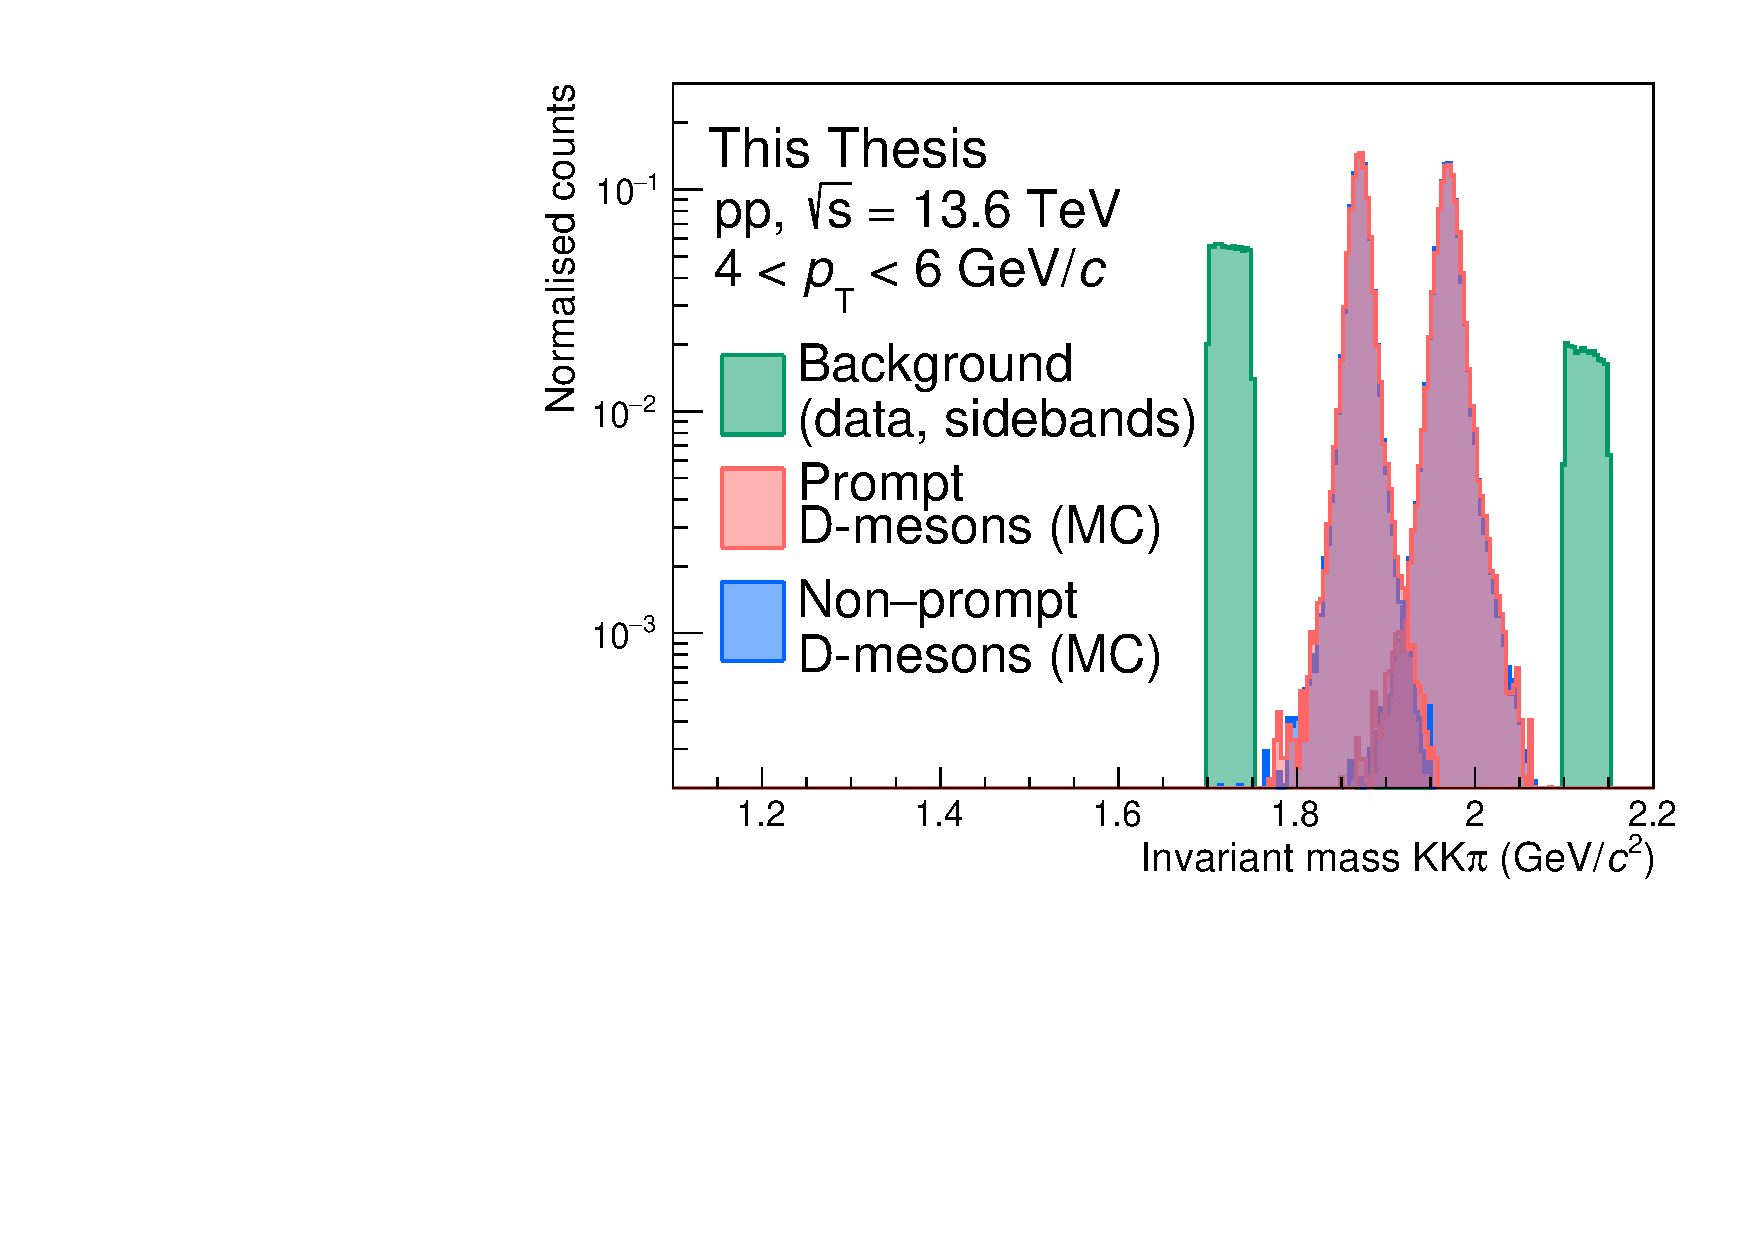
\includegraphics[width=0.7\textwidth]{Figures/Chapter 5/Mass.pdf}
    \caption{Invariant mass distribution of prompt and non-prompt D mesons (red and blue, respectively), taken from MC simulations, and of the background candidates taken from real data used to train the ML model (green) in the \mbox{$4<\pt<6$~\gevc} interval. Background candidates are selected in the \mbox{$1.7 < M < 1.75$~\gevcc} or \mbox{$2.1 < M < 2.15$~\gevcc} invariant-mass interval.}
    \label{fig:ml_training_mass}
\end{figure}

To reduce the amount of combinatorial background in the data samples prior to the application of ML-based selections, some loose selections were applied. These pre-selections are very effective at rejecting the combinatorial background, while preserving the selection efficiency for \ds and \dpl mesons, and are reported in Table~\ref{tab:presel}. These criteria include selections on the invariant mass of the $\mathrm{KK\pi}$ triplet to reduce the number of candidates to those necessary for the invariant mass analysis. To separate signal and background, topological variables such as the decay length $L$ and the cosine of the pointing angle $\cos\theta_\mathrm{p}$, introduced in Sec.~\ref{sec:topologicalSelections}, and PID variables, introduced in Sec.~\ref{sec:PIDselections} were applied. The selection criterion on the $n\sigma_\mathrm{TOF}$ variable is applied only when a TOF cluster is matched to the track, i.e., tracks with no TOF signal are not rejected. In addition, a logical \code{OR} is applied to the conditions on the PID variables, meaning that a candidate is accepted if, for all daughter tracks, at least one of the conditions on the $n\sigma_\mathrm{TOF}$ and $n\sigma_\mathrm{TPC}$ is satisfied. A selection is also applied to the $\chi^2_\mathrm{PCA}$ variable, quantifying the dispersion of the decay tracks around the secondary vertex, normalised to their uncertainty.

\begin{table}[h!]
  \begin{center}
    \caption{Topological and kinematical pre-selections applied to the \ds- and \dpl-mesons candidates. The selection criterion on the $n\sigma_\mathrm{TOF}$ variable is applied only when a TOF cluster is matched to the track, i.e., tracks with no TOF signal are not rejected. In addition, a logical \code{OR} is applied to the conditions on the $n\sigma_\mathrm{TOF}$ and $n\sigma_\mathrm{TPC}$ PID variables, meaning that a candidate is accepted if, for all daughter tracks, at least one of the conditions is satisfied.}
    \vspace*{0.3cm}
    \label{tab:presel}
    \begin{tabular}{c|ccc}
        \toprule
        & \multicolumn{3}{c}{\pt interval~(\gevc)}\\
        \midrule
       Variable & 0.0$-$1.5 & 1.5$-$12 &  12$-$24\\
        \midrule
      $\lvert M - M_\ds^\mathrm{PDG} \rvert~(\mevcc) <$ & 400 & 400 & 400\\
      $\pt(\pi, \mathrm{K})~(\gevc) >$  & 0.3   & 0.4   & 0.4\\
      Decay length (cm) $>$             & 0.02  & 0.02  & 0.03\\
      Normalized decay length XY $>$      &2     & 2     & 2\\
      $\cos\theta_\mathrm{p}>$        & 0.85  & 0.85  & 0.85\\
      $\cos\theta_\mathrm{p}^{xy}>$            & 0.85  & 0.85  & 0.85\\
      $M^{\phi}_\mathrm{inv}$ - $M^{\phi~\mathrm{PDG}}_\mathrm{inv}~(\mevcc) <$ & 20 & 20 & 20\\
      $\chi^2_\mathrm{PCA} < $          & 10    & 10    & 10\\
      $\lvert n\sigma_\mathrm{TPC}\rvert <$                   & 5     & 5     & 5\\
      $\lvert n\sigma_\mathrm{TOF}\rvert <$                   & 5     & 5     & 5\\
      \bottomrule
    \end{tabular}
  \end{center}
\end{table}

Labels are assigned as a numerical value to each candidate, with 0 indicating a background candidate, 1 a prompt \ds meson, and 2 a non-prompt \ds meson.

The dataset is then divided into two different subsamples. The first comprehends 80\% of the data, and is used to train the model, while the remaining 20\% is used to test its performance. In addition, since the D-meson decay topology can significantly differ depending on the \pt of the meson due to different Lorentz boosts, the dataset is divided into several \pt intervals, and the model is trained and tested separately for each of them. To achieve a better performance of the ML models, they are trained in broader \pt intervals than those used for the analysis, to ensure that enough data is available to train a well-performing model. The total number of candidates available for training and testing the model is reported in Table~\ref{tab:training_sample} for the considered \pt intervals.


\begin{table}[tb]
    \begin{center}
    \caption{Number of candidates within the \pt intervals used to train and test the model.}
    \label{tab:training_sample}
    \vspace*{0.3cm}
    \begin{tabular}{c|c}
         \toprule
         \pt (\gevc) & Candidates\\
         \midrule         
         0--1.5     & $\sim 4.6 \times 10^{3}$  \\
         1.5--2     & $\sim 6.1 \times 10^{3}$ \\
         2--3       & $\sim 26  \times 10^{3}$  \\
         3--4       & $\sim 34  \times 10^{3}$  \\
         4--5       & $\sim 31  \times 10^{3}$ \\
         5--6       & $\sim 24  \times 10^{3}$ \\
         6--8       &  $\sim 22   \times 10^{3}$\\
         8--12      & $\sim 10   \times 10^{3}$\\
         12--24     & $\sim 2.6  \times 10^{3}$ \\
         \bottomrule
    \end{tabular}
    \end{center}
\end{table}

\begin{sloppypar}
To produce a balanced dataset, the number of candidates in each class is equalised to the number of examples in the minority class. This is achieved by randomly selecting a subset of the majority classes. The balanced dataset is then used to train the model.
\end{sloppypar}

The choice of features used to separate signal from background is crucial, as they must be able to discriminate between signal and background candidates, and must be chosen in such a way that no bias is introduced in the final result. The variables used to train the model were introduced in Chapter~\ref{chap:reconstruction}, and are a mixture of topological, kinematical, and PID variables. The key idea is to exploit the displaced topology of the D-meson decay, which is a distinctive feature of the signal candidates, the kinematic properties of the D-meson decay, and the PID information of the daughter tracks to discriminate between signal and background candidates. The features used to train the model are reported in Table~\ref{tab:ml_training_vars}. The number in parenthesis after $n\sigma$ indicates the prong identification number. The tracks are ordered based on their charge sign, so that the first and third prongs (prongs 0 and 2) are the like-sign tracks (i.e., their charge sign is the same as that of the D meson), while the second prong (prong 1) is the opposite-sign track.

\begin{table}[tb]
    \begin{center}
    \caption{Candidate features used to train the ML model.}
    \label{tab:ml_training_vars}
    \vspace*{0.3cm}
    \begin{tabular}{c}
         \toprule
         Variable\\
         \midrule         
         Cosine of pointing angle ($\cos\theta_\mathrm{p}$)\\
         Cosine of pointing angle XY ($\cos\theta_\mathrm{p}^{xy}$)\\
         Decay length ($L$)\\
         Decay length XY ($L^{xy}$)\\
         Candidate impact parameter XY ($d^{xy}$)\\
         $\lvert \cos^{3}\theta'(\mathrm K)\rvert$\\
         Prong 0 impact parameter XY ($d_{0}^{xy}$)\\
         Prong 1 impact parameter XY ($d_{1}^{xy}$)\\
         Prong 2 impact parameter XY ($d_{2}^{xy}$)\\
         $n\sigma_\mathrm{comb}^{\pi}(0)$\\         
         $n\sigma_\mathrm{comb}^{\pi}(1)$\\
         $n\sigma_\mathrm{comb}^{\pi}(2)$\\
         $n\sigma_\mathrm{comb}^{\mathrm K}(0)$\\
         $n\sigma_\mathrm{comb}^{\mathrm K}(1)$\\
         $n\sigma_\mathrm{comb}^{\mathrm K}(2)$\\
         \bottomrule
    \end{tabular}
    \end{center}
\end{table}

The invariant mass of the candidate and its \pt are excluded from the model training to prevent any bias in the final results. Including these variables would cause the model to preferentially select candidates within a specific invariant mass range (corresponding to that of \ds and \dpl mesons) or \pt, thereby skewing both candidate selection and the \pt distribution of the final sample, resulting in a biased \pt-differential yield. While it is possible to correct for a \pt-dependent selection using MC simulations, this approach is not taken here to avoid biases from any inaccuracies in the \pt distribution of the D mesons in the simulations. 

Some of the variables used to train the model may be correlated with the invariant mass of the candidate, and the ML may learn to discriminate the signal from the background by exploiting this correlation with the \ds meson mass and transverse momentum, rather than the physical properties of the signal and background. To exclude this possibility, the correlation between the features used to train the model is studied. To quantitatively describe the correlation between the variables, the Pearson correlation coefficient $\rho$ is evaluated for each pair of variables. It is defined as the ratio between the covariance of two variables $x$ and $y$ and the product of their standard deviations, $\rho(x,y) = \mathrm{cov}(x,y)/(\sigma_{x}\sigma_{y})$. It expresses the strength and direction of a linear correlation between two variables, ranging from $\rho = 1$ (perfect positive linear correlation) to $\rho = -1$ (perfect negative linear relationship). $\rho = 0$ indicates the absence of linear correlation.


\begin{sloppypar}
The correlation matrix of the features used to train the model is shown in Fig.~\ref{fig:ml_training_vars} for the prompt \ds, non-prompt \ds and background classes, in the \mbox{$2<\pt<3$~\gevc} interval of D-meson transverse momentum. The correlation with the invariant mass and the transverse momentum is also reported. The Pearson coefficient is encoded in the colour of the cell, with red indicating a positive correlation, blue a negative correlation, and grey no linear correlation. The correlation matrix shows that the variables used to train the model are not linearly correlated with the invariant mass of the candidate, suggesting that a ML model should not modify the invariant-mass distribution of the selected candidates.
\end{sloppypar}

Variables carrying similar physical information, such as those related to the candidate decay length, pointing angle, and impact parameter, are strongly correlated among each other, as expected. Different degrees of correlation between the same variable pairs are observed for the different classes. The ML model can exploit these differences to discriminate between the three classes of candidates.

\begin{figure}[p]
    \centering
    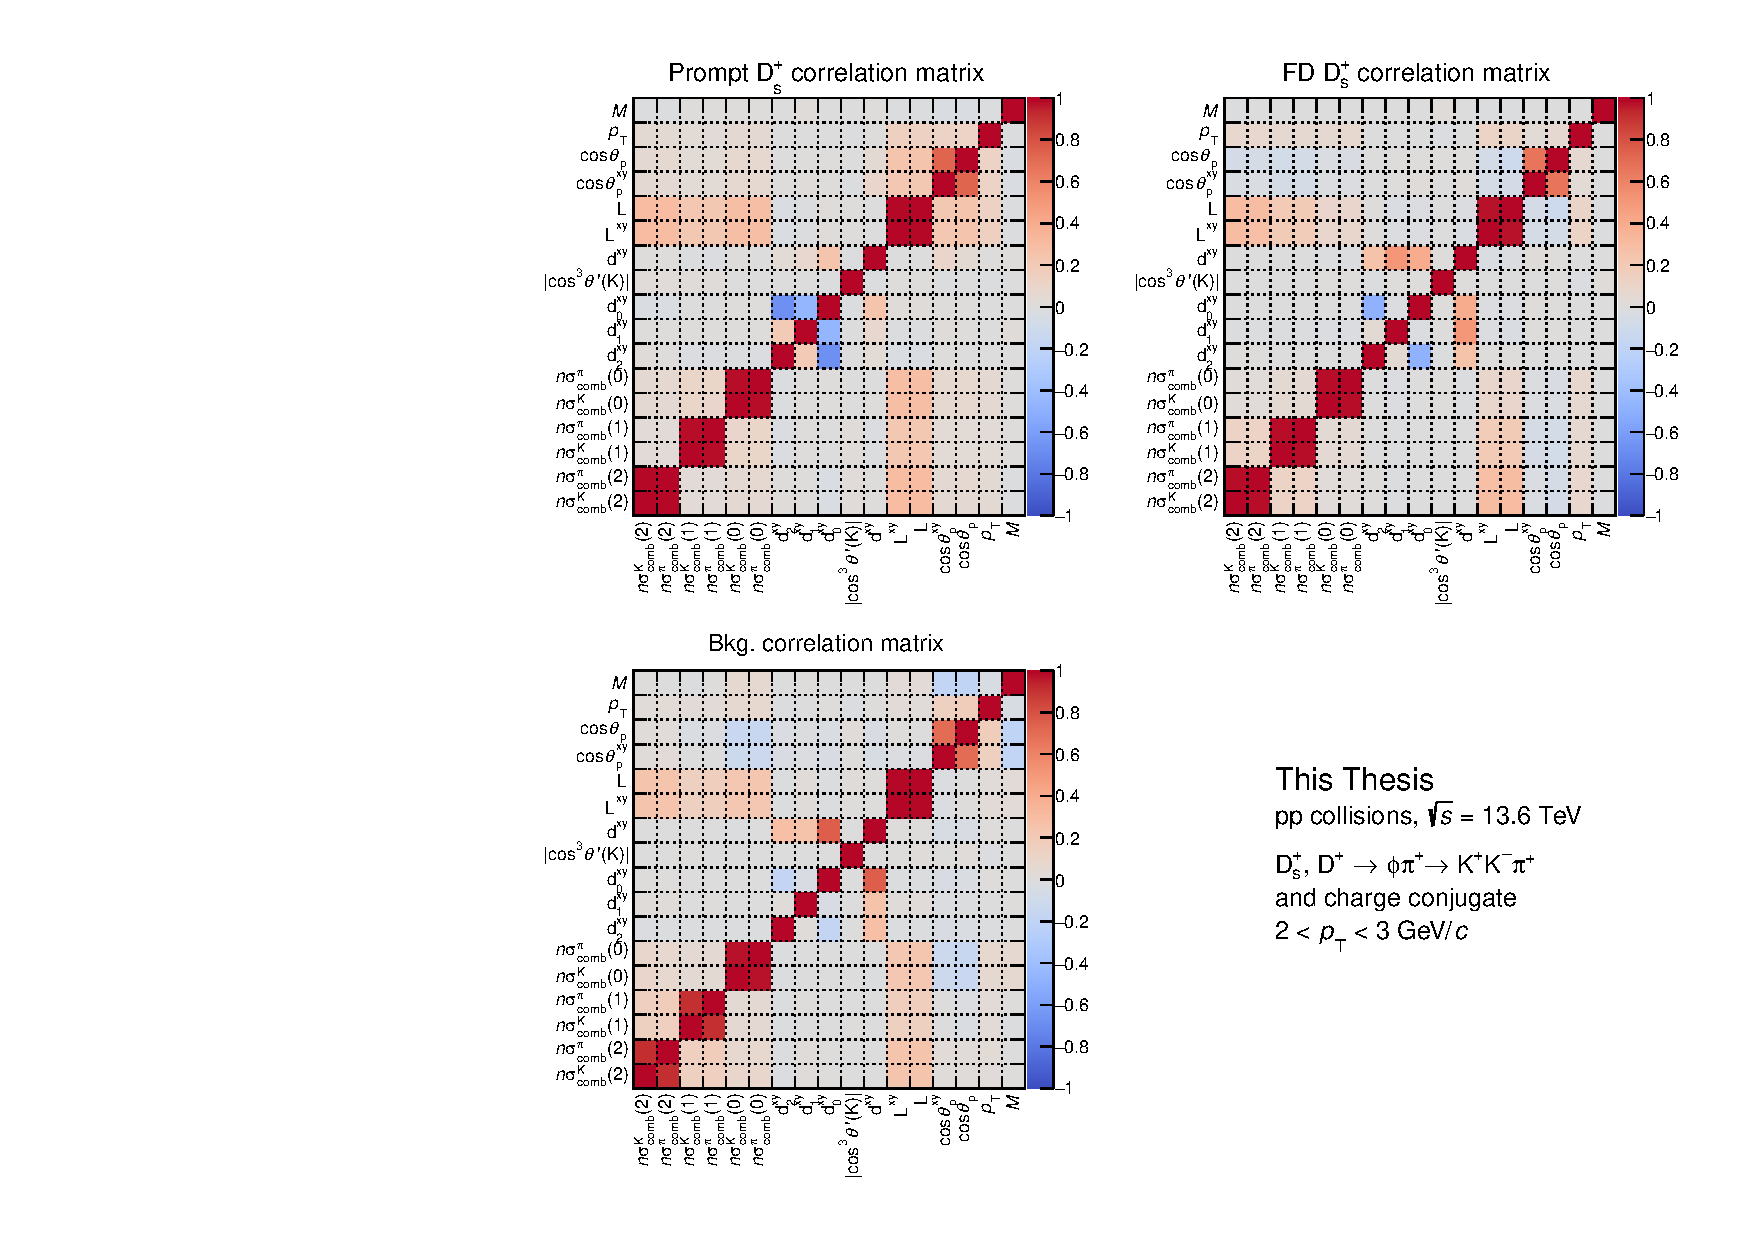
\includegraphics[width=\textwidth]{Figures/Chapter 5/CorrelationMatrix.pdf}
    \caption{Correlation matrices of the features used to train the ML model for prompt \ds (top-left), non-prompt \ds (top-right), and background (bottom-left) candidates in the $2<\pt<3$~\gevc interval. The correlation with the invariant mass and the transverse momentum is also reported. The Pearson coefficient is encoded in the colour of the cell, with red indicating a positive correlation, blue a negative correlation, and grey no linear correlation.}
    \label{fig:ml_training_vars}
\end{figure}

\subsection{Boosted Decision Trees}
Once the training dataset has been composed and the features have been selected, the ML architecture has to be chosen. Several algorithms are available, each with its own strengths and weaknesses. The choice of the algorithm depends on the specific problem to solve, the size of the dataset, and the computational resources available. 

Boosted decision trees~\cite{friedman2001greedy,freund1997decision} (BDTs) are a family of machine learning algorithms employed in different fields, including high-energy physics. Their building blocks are decision trees, which are a versatile type of supervised learning algorithm that can be used for both classification and regression tasks. A decision tree is made of many \emph{nodes}, each containing conditions that split the data into two~\cite{breiman2017classification} or more~\cite{quinlan1986induction} children nodes. The first node of the tree, which receives all the data, is called \emph{root} node, while nodes that do not further split the data are called \emph{leaves}, and contain the output of the tree. The model is trained by considering the Gini index, which measures the impurity of the node:
\begin{equation*}
    G = 1 - \sum_{i=1}^{n} p_{i}^{2}\quad ,
\end{equation*}
where $p_{i}$ is the fraction of samples in the node that belong to the class $i$. The Gini index therefore provides an indication of the quality of the split, with $G=0$ indicating a perfect split. A commonly used algorithm to build \emph{binary} decision trees (i.e., each node contains binary-output conditions, and is split into two children nodes) is the \emph{Classification And Regression Tree} (CART) algorithm~\cite{breiman2017classification}, which recursively splits the dataset into subsets based on a single feature $k$ and a threshold $t_k$ that minimises the impurity of the subsets (weighted by their size). The cost function that the algorithm tries to minimise is given by
\begin{equation*}
    J(k,t_k) = \frac{m_{\mathrm{left}}}{m}G_{\mathrm{left}} + \frac{m_{\mathrm{right}}}{m}G_{\mathrm{right}}\quad ,
\end{equation*}
where $m_{\mathrm{left}}$ and $m_{\mathrm{right}}$ are the number of samples in the left and right nodes, respectively, summing up to the total number of samples $m$, and $G_{\mathrm{left}}$ and $G_{\mathrm{right}}$ are the Gini indices of the left and right nodes. The tree is grown until a stopping criterion is met, such as a maximum depth, a minimum number of samples in a node, or a minimum impurity decrease. These are all hyperparameters that can be tuned to optimise the model's performance.

Given their simplicity, decision trees are fairly easy to interpret, and are often called \emph{white-box} models (in contrast to BDTs and neural networks, where the decision-making process is less transparent, therefore called \emph{black-box} models). An additional strength of decision trees is that they require
very little data preparation, e.g., they do not require feature scaling or centering, making them a very powerful yet simple tool for data analysis. However, they are prone to overfitting, as they can grow to a large depth, capturing the noise in the training data. To mitigate this issue, their depth can be constrained, but this may lead to a model with limited discrimination power. To build a robust model with a good discrimination power, ensemble methods may be used. Several decision trees can be trained, and the final prediction is obtained by combining the outcome of all the trees. 

\subsubsection{XGBoost}
In this work, the Extreme Gradient Boosting~\cite{DBLP:xgboost} (XGBoost) Boosted Decision Trees (BDT) algorithm is used. It has achieved state-of-the-art results in a number of machine learning and data mining challenges (for example in Ref.~\cite{kaggle:higgs}). In addition, this algorithm, which is available as an open-source package, can be easily parallelised on CPUs and GPUs~\cite{mitchell2017accelerating}, thereby reducing the training and application time.

The term \emph{boosting} refers to any ensemble method combining several weak learners into a strong learner. The general idea of most boosting methods is to train many predictors sequentially, each trying to correct its predecessor~\cite{geron2022hands}. The function estimate $\widehat{f}(x)$ is parametrised with an additive functional form:
\begin{equation*}
    \widehat{f}(x) = \sum_{\mathrm{k}=0}^{\mathrm{M}} \widehat{f}_\mathrm{k}(x)\quad ,
\end{equation*}
where M is the number of iterations, $\widehat{f}_\mathrm{0}(x)$ is the initial prediction, and $\widehat{f}_\mathrm{i}(x)$ is the function increment at the $i$-th iteration, also called \emph{boost}. To reduce the loss function, a new weak learner, whose functional form is parametrised as $h(x,\theta)$, can be added to the ensemble:
\begin{equation*}
    \widehat{f}_\mathrm{t}(x) \leftarrow \widehat{f}_{\mathrm{t}-1}(x) + \rho_\mathrm{t} h(x,\theta_\mathrm{t})\quad .
\end{equation*}
$\rho_t$ is the step size, which is optimised for each iteration t, together with the parameters $\theta_\mathrm{t}$ of the weak learner:
\begin{equation*}
    (\rho_\mathrm{t}, \theta_\mathrm{t}) = \arg\min_{\rho,\theta} \sum_{{i}=1}^{\mathrm{N}} L\left(y_i, \widehat{f}_{\mathrm{t}-1}(x_i) + \rho h(x_i,\theta)\right)\quad ,
\end{equation*}
where $L$ is the loss function, and $y_i$ is the true label of the i-th example. Despite having a well-defined set of equations for minimising the loss function, the optimisation of the parameters is not trivial, as the loss function is non-convex and the search space is high-dimensional. Therefore, the optimisation is usually performed using a gradient-based algorithm~\cite{friedman2001greedy,natekin2013gradient}, where $h(x,\theta_\mathrm{t})$ is chosen as the most parallel function to the negative gradient of the loss function with respect to the previous prediction $g_\mathrm{t}(x)$:
\begin{equation*}
    g_\mathrm{t}(x) = E_{\mathbf{y}}\left[ \frac{\partial L(\mathbf{y},\widehat{f}_{\mathrm{t}-1}(x))}{\partial \widehat{f}_{\mathrm{t}-1}(x)} \Bigg{|} x \right] \quad ,
\end{equation*}
where $E_{\mathbf{y}}$ is the expectation over the true labels. The parameters are then optimised by minimising the difference between the negative gradient and the weak learner prediction:
\begin{equation*}
    (\rho_\mathrm{t}, \theta_\mathrm{t}) = \arg\min_{\rho,\theta} \sum_{\mathrm{i}=1}^{\mathrm{N}} \left[-g_\mathrm{t} - \rho h(x_\mathrm{i},\theta)\right]^{2}\quad .
\end{equation*}

Through the iterative addition of weak learners, the loss function is reduced and the model learns the complex patterns of data. The final prediction is obtained by summing the predictions of all the weak learners. In the XGBoost algorithm, the weak learners are decision trees. The output consists of a numerical score for each class, ranging from 0 to 1 and summing up to unity. Each score represents the confidence of the model in the prediction, which can be interpreted as the probability of the example belonging to that class.
\subsection{Tuning the model's hyperparameters}
The XGBoost algorithm has several hyperparameters~\cite{XGBoost_parameters} that can be tuned to optimise the model's performance. The most important hyperparameters are:
\begin{itemize}
    \item \code{eta} or \code{learning\_rate}, which is the step size shrinkage of the gradient descent algorithm. To reduce the risk of overfitting, this factor multiplies the weak-learner prediction ($\rho_\mathrm{t} h(x_\mathrm{i},\theta) \rightarrow \code{eta} \cdot \rho_\mathrm{t} h(x_\mathrm{i},\theta)$), and is usually set to a small value, such as 0.1;
    \item \code{max\_depth}, which is the maximum depth of a single decision tree. A large depth can lead to overfitting, while a small depth can lead to a model with limited discrimination power. Usually, this parameter is set to around 5;
    \item \code{n\_estimators}, which defines the number of trees to train. A large number of weak learners can lead to overfitting, while a small number can lead to a model with limited discrimination power. Usually, the number of weak learners is set to around 1000;
    \item \code{subsample}, which is the fraction of the training data to be used to train each tree at each iteration;
    \item \code{min\_child\_weight}, which is the minimum sum of instance weight needed in a child. It is related to the purity in a node, and it is used to stop the tree growth;
    \item \code{colsample\_bytree}, which is the fraction of features to be used to train each tree at each iteration;
    \item \code{tree\_method}, which defines the algorithm used to build the trees. The \code{hist} option uses an optimised histogram-based algorithm and is usually the fastest.
\end{itemize}

The hyperparameters are optimised using the Optuna framework~\cite{akiba2019optuna}, which proved to be a powerful tool thanks to its state-of-the-art algorithms for sampling the hyperparameter space and for efficiently pruning unpromising trials. The Tree-Structured Parzen Estimator~\cite{bergstra2011algorithms}, is used in this Thesis. It is a Bayesian optimisation algorithm able to explore the hyperparameter space efficiently. The aim of a Bayesian optimisation is to maximise (or minimise, depending on the task) an objective function $f(\mathbf{x})$ by iteratively sampling a bounded hyperparameter space, $\chi$. The algorithm builds a probabilistic model of the objective function, and uses it to decide which hyperparameters to sample next. The model is updated at each iteration, and the hyperparameters that are most likely to improve the model's performance are sampled. The Optuna algorithm is also able to prune unpromising trials, reducing the computational cost of the optimisation. The optimisation is performed using a 5-fold cross-validation, and the hyperparameters that maximise the macro-averaged one-vs-one Receiver Operating Characteristic Area Under the Curve (ROC AUC) metric (described in detail in Sec.~\ref{sec:ml_performance}) are chosen as the optimal configuration. The hyperparameters optimised for the XGBoost model are reported in Table~\ref{tab:ml_hyperparameters} for some representative \pt intervals considered in the model training. An additional hyperparameter, \code{lambda}, which is the $\mathrm{L_2}$ regularisation term, is also optimised. It helps to prevent overfitting by penalising overly complex models. The optimal hyperparameters are then used to train the model on the full training dataset.

\begin{table}[tb!]
    \centering
    \caption{Optimised hyperparameter configuration for some representative \pt intervals considered in the model training.}
    \label{tab:ml_hyperparameters}
    \vspace*{0.3cm}
    \resizebox{\columnwidth}{!}{%
    \begin{tabular}{c|cccccc}
         \toprule
         Hyper-parameter & \multicolumn{6}{c}{$\pt$ interval (\gevc)} \\
         \midrule
            & 0--1.5 & 1.5--2 & 2--3 & 4--5 & 6--8 & 12--24 \\
        \midrule
         \code{max\textunderscore depth} & 3 & 3 & 3 & 3 & 3 & 3\\

         \code{learning\textunderscore rate} & 0.04 & 0.068 & 0.065 & 0.091 & 0.070 & 0.030\\
         
         \code{n\textunderscore estimators} & 473 & 339 & 1352 & 1256 & 1142 & 1188\\ 
         
         \code{min\textunderscore child\textunderscore weight} & 1 & 3 & 10 & 10 & 3 & 5\\
         
         \code{subsample} & 0.87 & 0.95 & 0.84 & 0.95 & 0.81 & 0.88\\
         
         \code{colsample\textunderscore bytree} & 0.91 & 0.98 & 0.90 & 0.96 & 0.88 & 0.89\\

         \code{lambda} & $8.0\times10^{-4}$ & $4.8\times10^{-4}$ & $9.1\times10^{-4}$ &  $3.0\times10^{-4}$ & $1.9\times10^{-4}$ & $6.7\times10^{-4}$\\
         $\code{tree\textunderscore method}$ & $\code{hist}$& $\code{hist}$& $\code{hist}$ & $\code{hist}$ & $\code{hist}$& $\code{hist}$\\
         \bottomrule
    \end{tabular}%
}
\end{table}

\subsection{Evaluation of the model's performance}\label{sec:ml_performance}
After training the model, its performance is evaluated on the test dataset. The model's performance can be assessed using a \emph{confusion matrix}, which summarises the number of examples for a given class (the true label) that are classified by the model as belonging to any of the available classes (the predicted label). A good model should provide a high number of correctly-classified examples (reported on the diagonal of the confusion matrix), and a low number of misclassified examples (off-diagonal elements of the confusion matrix). The confusion matrix also allows an understanding of which classes are more difficult to classify, and which classes are more likely to be confused with each other. An example of a confusion matrix is shown in Fig.~\ref{fig:ml_confusion_matrix} for the XGBoost model trained on the $2<\pt<3$~\gevc interval.

\begin{figure}
    \centering
    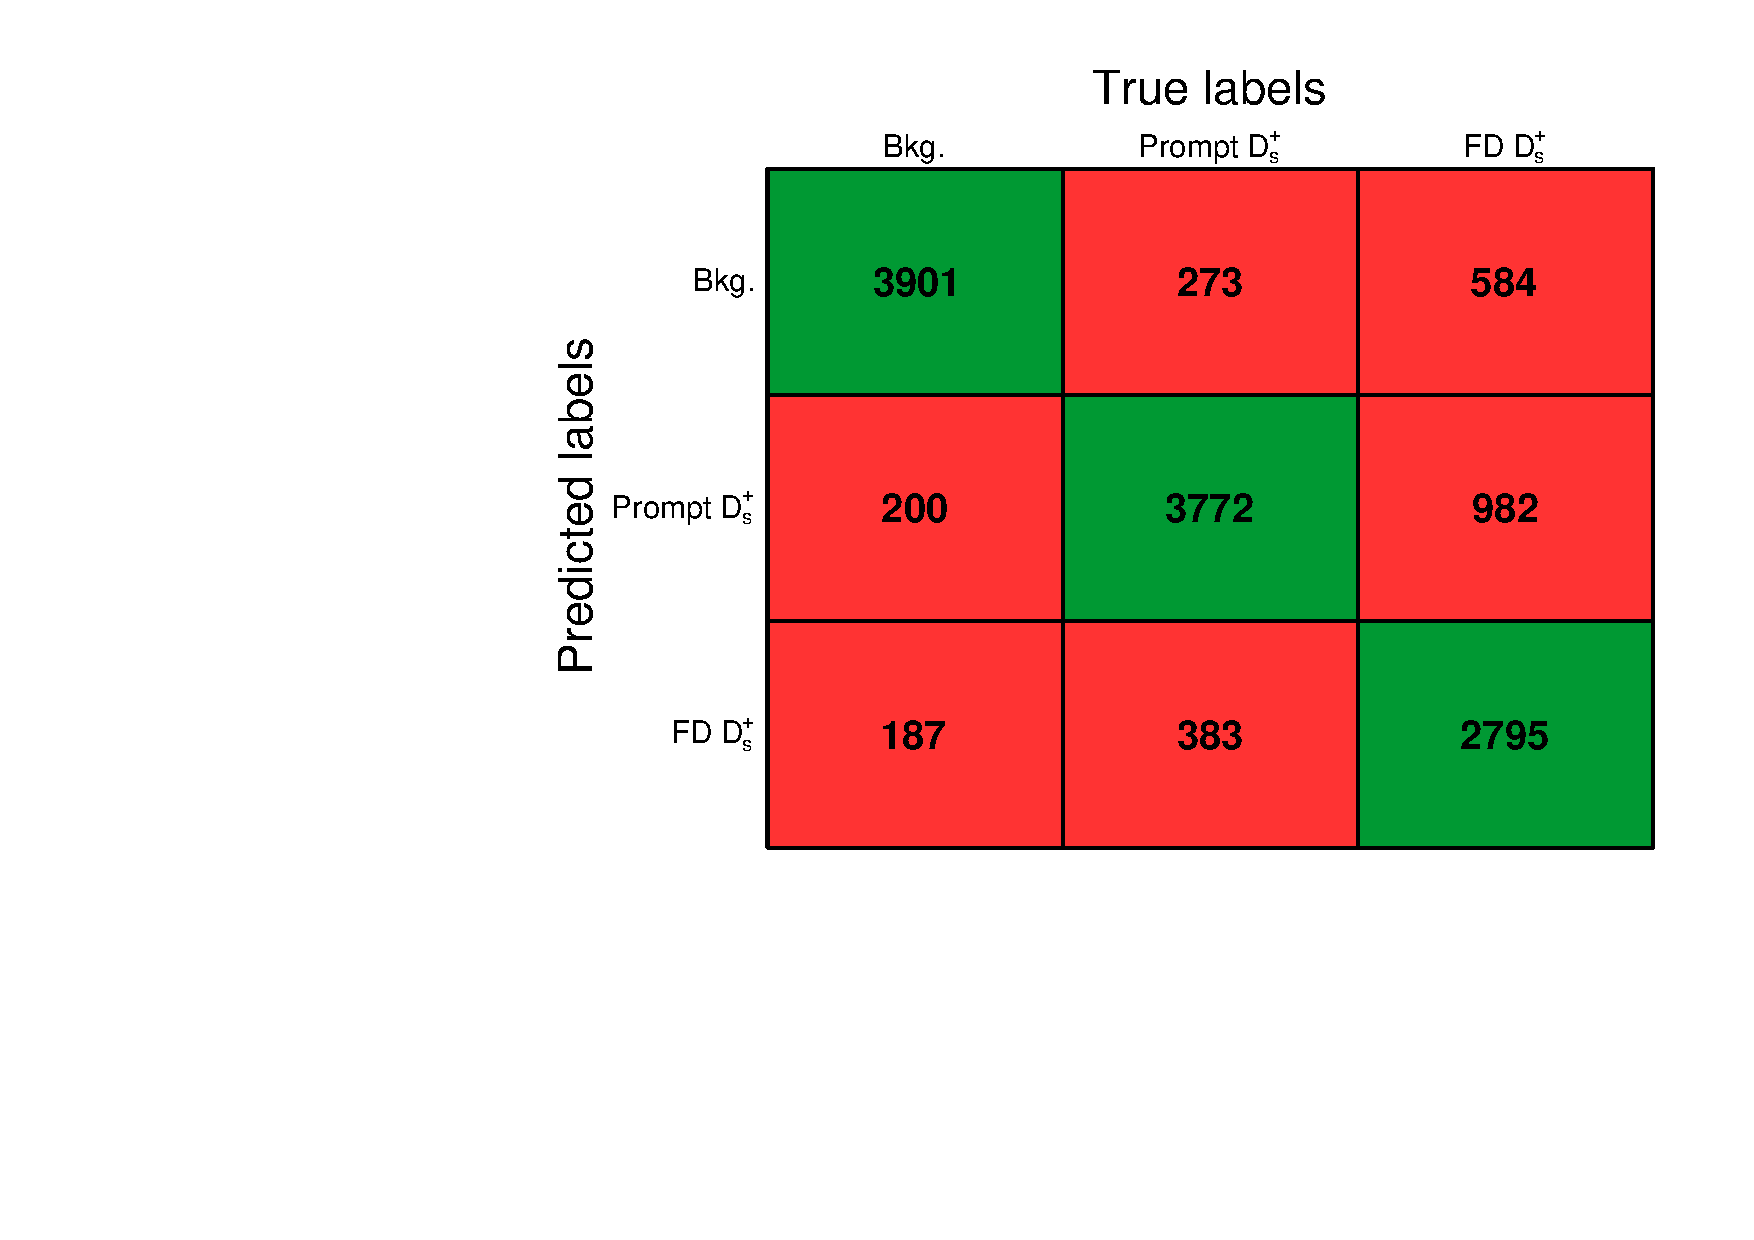
\includegraphics[width=0.7\textwidth]{Figures/Chapter 5/ConfusionMatrix.pdf}
    \caption{Confusion matrix for the BDT model trained in the \mbox{$2<\pt<3$~\gevc} interval. Candidates are classified as the class with the highest score.}
    \label{fig:ml_confusion_matrix}
\end{figure}

Despite providing a lot of information on the model's performance, more concise metrics of the model's performance are usually used, for a more direct comparison between different models. In addition, the confusion matrix provides a threshold-dependent measure of the model's performance, as the classification threshold (i.e., the threshold on the model output that defines the separation between the different classes) can be varied to increase the number of correctly classified signal candidates at the expense of the number of correctly classified background candidates, and vice versa. 

In binary classification tasks, where only two classes are available (a positive and a negative class), several metrics can be defined from the elements of the confusion matrix. The $2\mkern-2mu\times\mkern-2mu2$ confusion matrix contains four entries: the true positives (TP), which are the number of correctly classified positive candidates, the false positives (FP), which are the number of negative candidates being mistakenly classified as positives, and the analogously defined true negatives (TN) and false negatives (FN). One of the most used tools for binary classifiers is the \emph{Receiver Operating Characteristic} (ROC) curve, which represents the true positive rate (TPR) against the false positive rate (FPR) for different threshold values. The TPR is the fraction of correctly classified positive candidates ($\mathrm{TPR = TP/(TP+FN)}$), while the FPR is the fraction of incorrectly classified negative candidates ($\mathrm{FPR = FP/(FP+TN)}$). 

The output of the ML model is a single value ranging from 0 to 1 for a binary classification task, and can be interpreted as the probability of the candidate belonging to the positive class. If positive candidates are selected as those with a score greater than a certain threshold $t$, when $t=0$ all candidates are classified as positive, and both the TPR and FPR will be equal to 1. On the other hand, if $t=1$, no candidate is classified as positive, and the TPR and FPR will both equal 0. Therefore, the different values of $t$ between 0 and 1, which yield different TPR and FPR values, will trace the ROC curve, going from the point (1,1) to (0,0) as $t$ increases. The ROC \emph{Area Under the Curve} (AUC), is used to measure the model's ability to discriminate between positive and negative candidates, for any given threshold. The ROC AUC ranges from 0 to 1. A random classifier has a ROC AUC of 0.5, while a perfect classifier has a ROC AUC of 1. The ROC AUC is a threshold-independent measure of the model's performance, and is often used to compare different models. 

In a multiclass classification task, where more than two classes are available, a generalisation of the ROC curve and the ROC AUC metric is required. In this case, the \emph{One-vs-One} ROC curve~\cite{hand2001simple} can be defined as a plot of the TPR against the FPR for a given pair of classes. The One-vs-One ROC AUC can be averaged to the \emph{macro-averaged} One-vs-One ROC AUC, which is the average of the ROC AUC for each pair of classes and can provide a measurement of the model's ability to discriminate between all the classes. For a classification problem with N classes, there are $\mathrm{N(N-1)}$ possible pairs of ordered classes, and therefore of One-vs-One ROC curves. 


The One-vs-One ROC curves for the model trained on the $2<\pt<3$~\gevc interval are shown in Fig.~\ref{fig:ml_roc_curve}. The ROC AUC is calculated for each class pair, and is reported in the legend. Given that the classification task is a three-class problem, the One-vs-One ROC AUC is calculated for the three possible pairs of classes. Furthermore, despite showing an approximate symmetry around the line $\mathrm{TPR=1-FPR}$, the ROC curve for the A-vs-B pair is not exactly the symmetrical curve of the ROC curve of the B-vs-A pair when more than two classes are considered, due to the different probability of misclassification with the remaining classes. Therefore, two curves are shown for each pair of classes, and present different ROC AUC values. The metric is evaluated on both the training and test sets to test the model's generalisation power. The model's performance is excellent, with a macro-averaged One-vs-One ROC AUC value of 0.965, very close to that of an ideal classifier of 1. In addition, little overfitting is observed, as the ROC AUC values for the training and test sets are similar. The macro-averaged One-vs-One ROC AUC presents similar values in the other \pt intervals, indicating that the model's performance is stable across the studied \pt range. A slight increase in the ROC AUC of a few percent is observed for increasing \pt, due to the more displaced decay topology, which facilitates the separation of the three classes. In the highest \pt intervals the ROC AUC decreases due to the limited number of candidates in the training sample, which can lead to a less performant model. The model is then used to select \ds- and \dpl-meson candidates from the full dataset. 

\begin{figure}[htb]
    \centering
    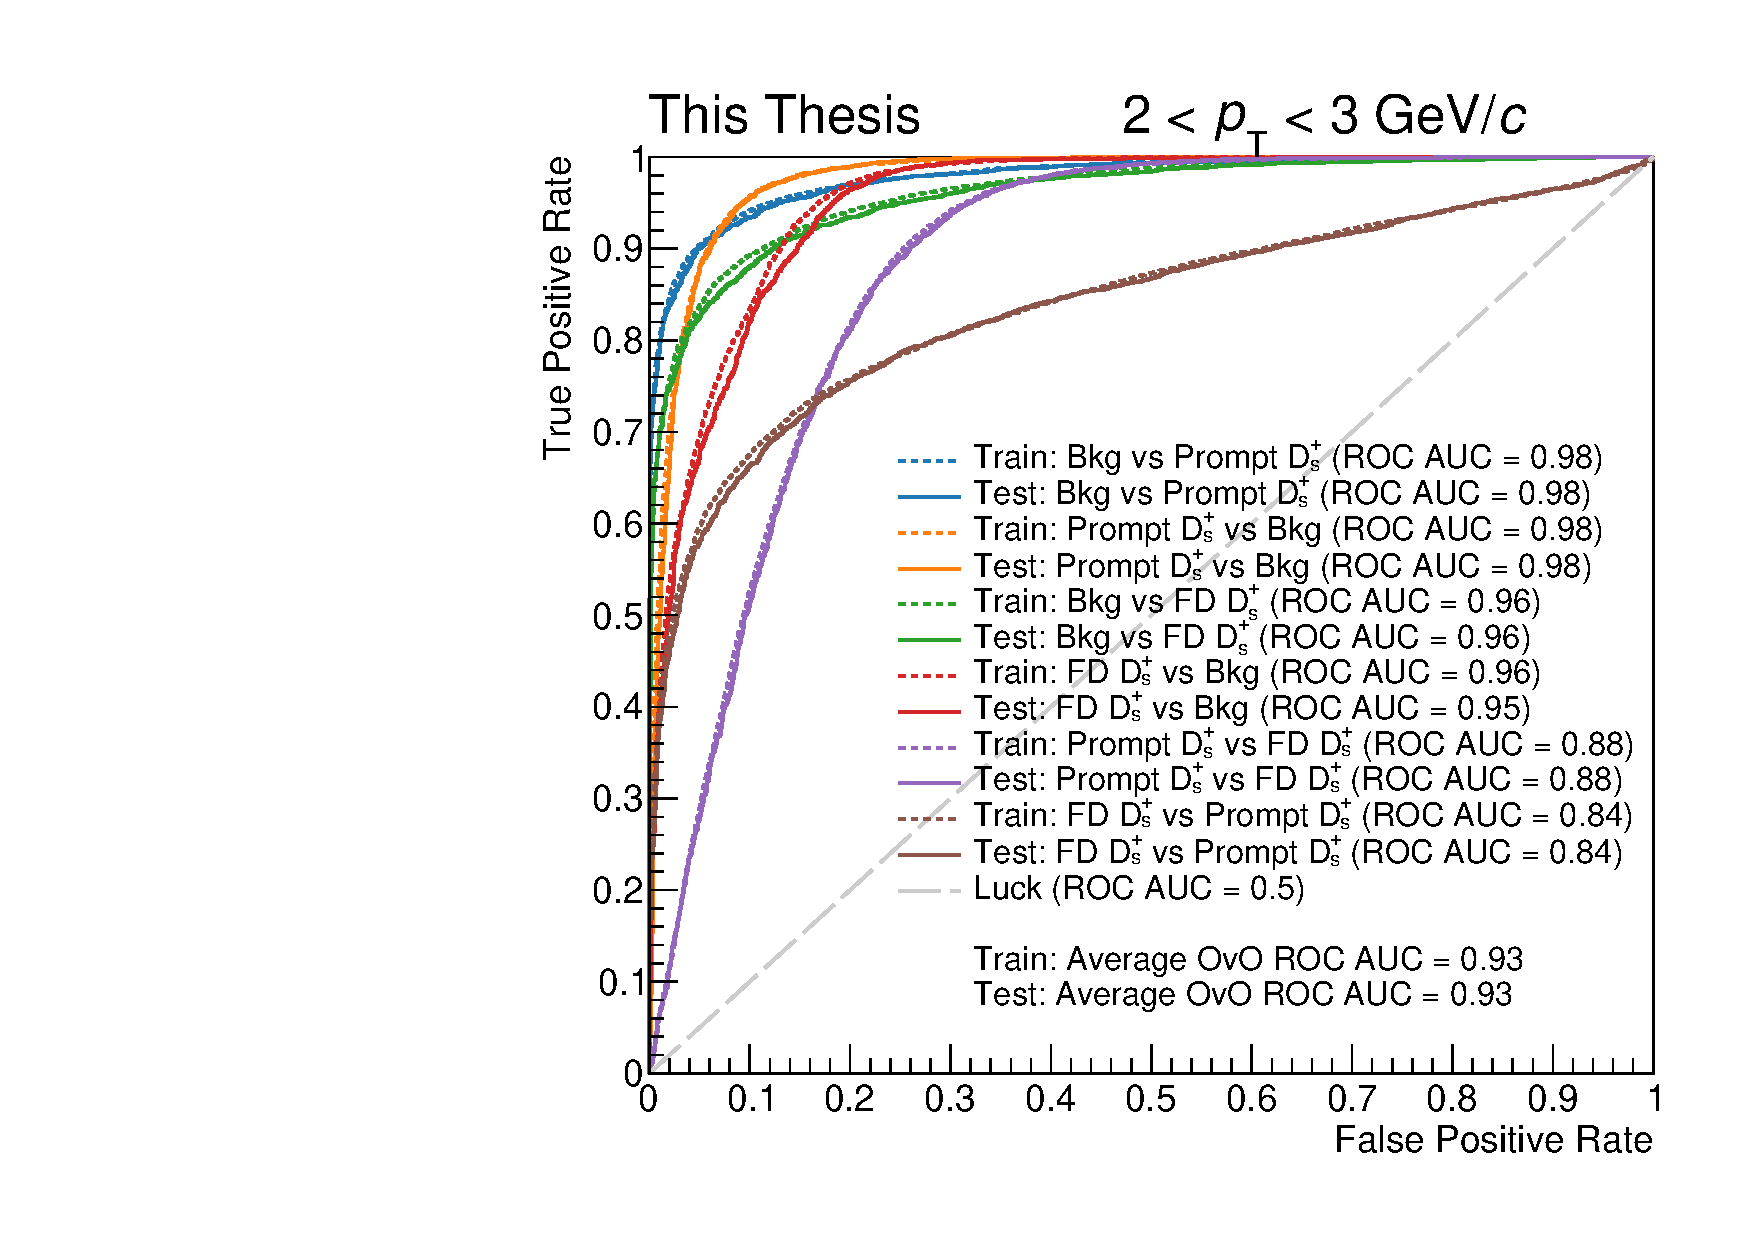
\includegraphics[width=0.7\textwidth]{Figures/Chapter 5/ROC.pdf}
    \caption{ROC curves for the model trained on the $2<\pt<3$~\gevc interval. The One-vs-One ROC AUC metric is calculated for each class pair and reported in the legend.}
    \label{fig:ml_roc_curve}
\end{figure}

\begin{sloppypar}
In addition to the ROC AUC, the model's performance can be evaluated by studying the distribution of the probability of belonging to a given class assigned to labelleled candidates. The score distributions for the model trained on the \mbox{$2<\pt<3$~\gevc} interval are shown in the three panels of Fig.~\ref{fig:ml_score} for the background, prompt \ds-meson, and non-prompt \ds-meson classes. For each class, the score distribution is shown for candidates belonging to the three different classes and to both the training and test sets. The distribution of the true background score provides interesting information on the model's performance. The score distribution for the background candidates peaks at high values, while the score distribution for the signal candidates (both prompt and non-prompt \ds meson) peaks at low values. This highlights that the model has effectively learned to discriminate between signal and background candidates, with good separation power. Furthermore, the score distributions for the training and test sets are fairly similar, indicating that the model generalises well to unseen data. Since non-prompt \ds mesons present a more displaced topology than promptly produced ones, due to the large lifetime of beauty-hadrons, the separation between non-prompt \ds mesons and background is noticeable in the non-prompt \ds-meson score distribution, where the score of true background candidates peaks at zero and the one of non-prompt \ds-meson candidates peaks at one. The distribution of prompt \ds mesons, which have a smaller displacement as compared to non-prompt ones falls in between those of background and non-prompt \ds mesons. Lastly, the separation between the three classes is less pronounced in the prompt \ds-meson score distribution, where the prompt \ds-meson distribution peaks at values significantly lower than one. Similar trends are observed in the other studied \pt intervals. 
\end{sloppypar}

\begin{figure}[p]
    \centering
    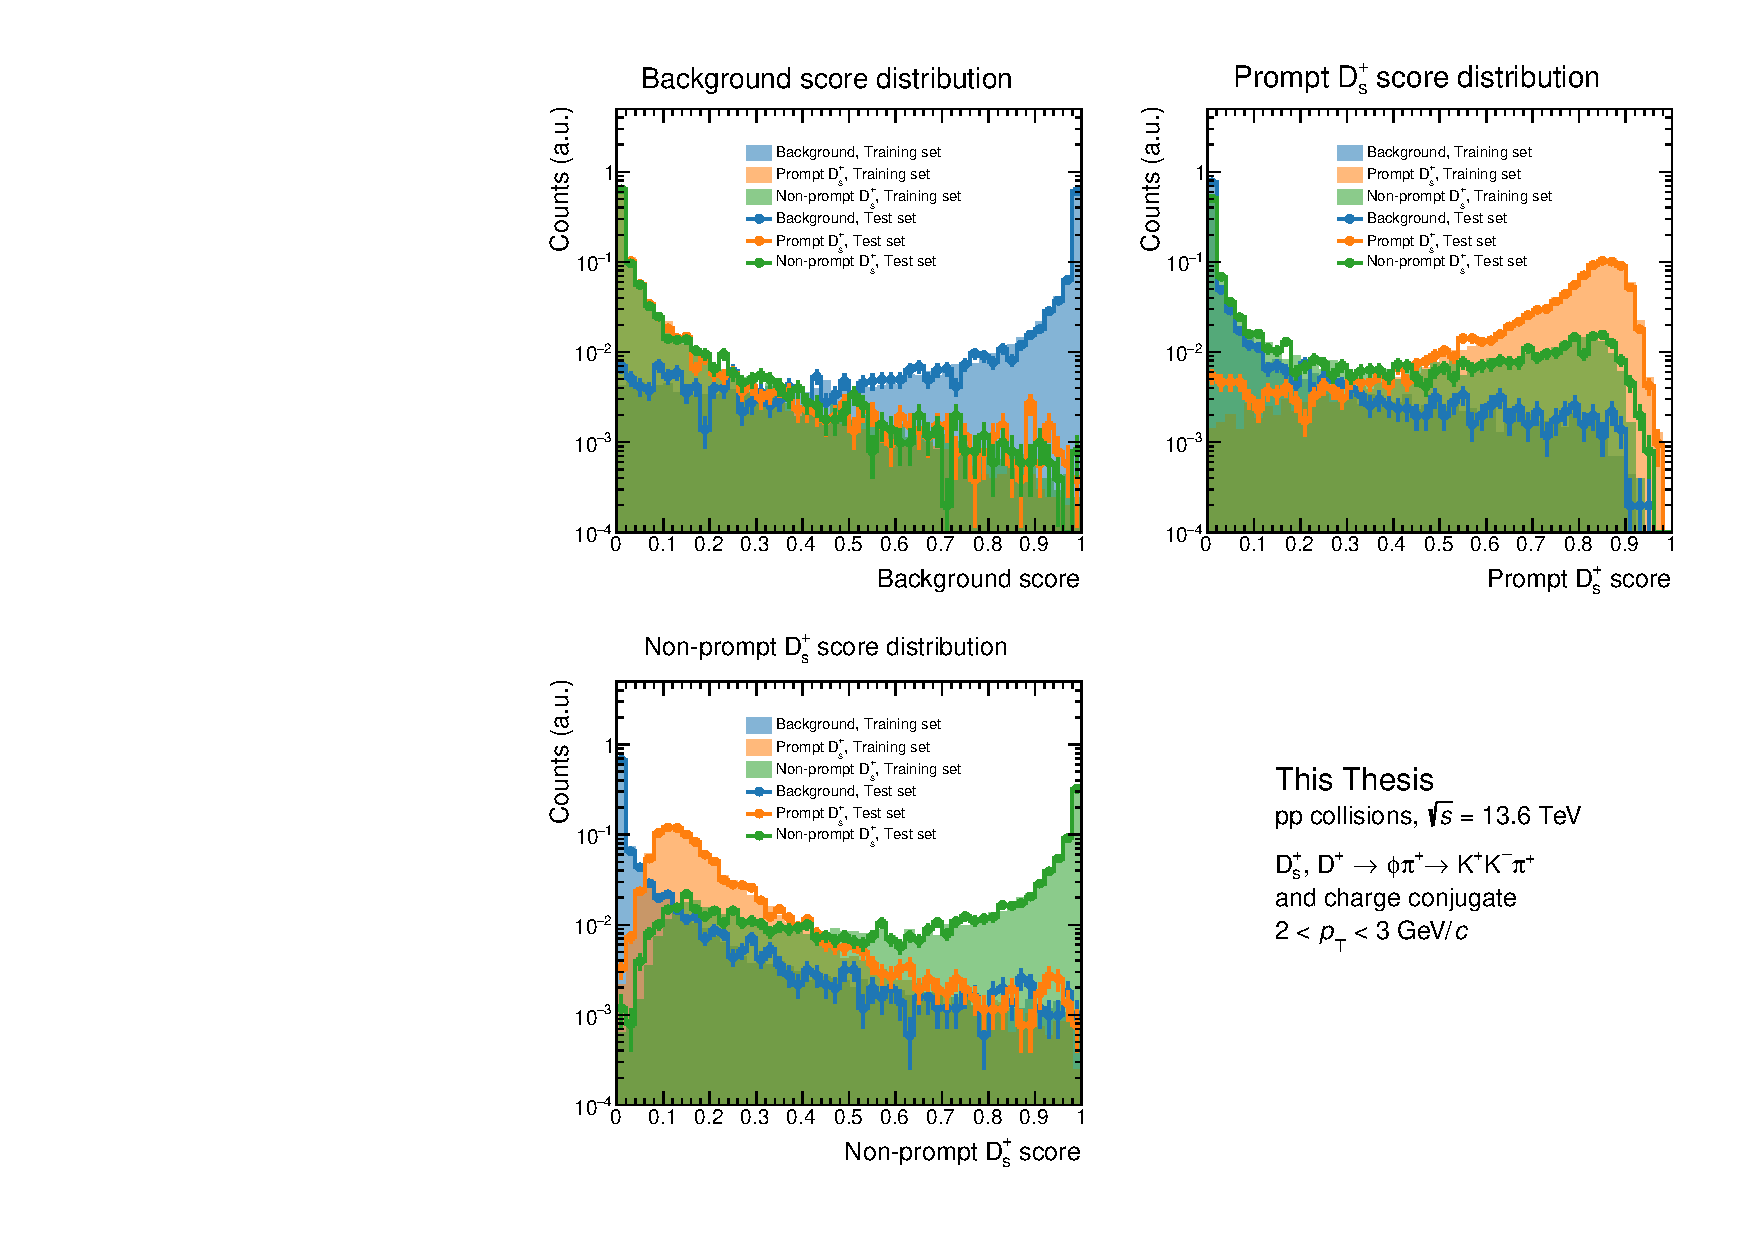
\includegraphics[width=\textwidth]{Figures/Chapter 5/Distributions.pdf}
    \caption{Score distributions for the model trained on the $2<\pt<3$~\gevc interval. The score distributions related to the probability of belonging to the background (top-left panel), prompt \ds-meson (top-right panel), and non-prompt \ds-meson (bottom-left panel) classes are shown. For each class, the score distribution is shown for candidates belonging to the different classes and to both the training (filled area) and test sets (markers).}
    \label{fig:ml_score}
\end{figure}

\subsection{Interpretation of the model's output: Feature importance}
The usage of ML algorithms usually provides a better performance in terms of signal-to-background separation as compared to approaches based on ``rectangular'' cuts, but it also introduces a level of complexity in the selection process. One of the most difficult aspects of using ML models is the interpretation of their output. To understand how the model makes its decisions, the feature importance can be studied. This allows the understanding of which features are more important for the model's decision-making process, and the optimisation of the feature selection. In addition, the feature importance can be used to check whether the model is learning on the correct features in terms of the physics of the problem.

One of the most used algorithms for feature importance studies is the SHapley Additive exPlanations~\cite{lundberg2017unified} (SHAP) algorithm. SHAP is a game-theoretic approach to explain the output of any machine learning model. It is based on the Shapley value~\cite{lipovetsky2001analysis} from cooperative game theory, which requires retraining the model on all feature subsets $\mathcal{S}\subseteq \mathcal{F}$, where $\mathcal{F}$ is the set of all features. An importance value is assigned to each feature i, representing the effect on the model prediction of including that feature. To compute this effect, a model $\widehat{f}_{\mathcal{S}\cup\{i\}}$ is trained with that feature present, and another model $\widehat{f}_\mathcal{S}$ is trained with the feature withheld. Then, predictions from the two
models are compared on the current input \mbox{$\widehat{f}_{\mathcal{S}\cup\{i\}} (x) - \widehat{f}_\mathcal{S}$}. The Shapley values are then computed as the weighted average of all possible differences:
\begin{equation*}
    \phi_\mathrm{i} = \sum_{\mathcal{S}\subseteq \mathcal{F}\setminus\{i\}} \frac{|\mathcal{S}|!(|\mathcal{F}|-|\mathcal{S}|-1)!}{|\mathcal{F}|!} \left[\widehat{f}_{\mathcal{S}\cup\{i\}}(x) - \widehat{f}_\mathcal{S}(x)\right]\quad .
\end{equation*}
Since most models cannot handle arbitrary patterns of missing input values, $\widehat{f} (z_\mathcal{S})$ is approximated with $E[\widehat{f}(z) | z_\mathcal{S}]$, where $z_\mathcal{S}$ is the input missing the features in $\mathcal{S}$. SHAP values therefore explain how to get from the base value $E[\widehat{f}(z)]$, which would be predicted if no features were known, to the output $\widehat{f}(x)$.

A beeswarm-style SHAP feature importance plot for the prompt \ds-meson probability predicted by the model trained in the $2<\pt<3$~\gevc interval is shown in Fig.~\ref{fig:ml_feature_importance}. In this plot, each instance is represented by a single dot on each feature row. The position of the dot along the horizontal axis is determined by the SHAP value of that feature, and the dots ``pile up'' along each feature row, to provide information on the distribution of the SHAP values. The colour of the dot represents the value of the feature, with blue indicating a low value and red a high value. Positive values indicate that the feature is pushing the model's prediction towards the prompt \ds-meson class, while negative values indicate that the model is less likely to classify the candidate as a prompt \ds meson. Feature rows are ordered from top to bottom based on the mean absolute value of the SHAP values for that feature, with the most important features, i.e., those with the highest impact on the model's decision, at the top. The most important features are the cosine of pointing angle $\cos\theta_\mathrm{p}$, the decay length $L$, the decay length in the XY plane $L^{xy}$, the absolute value of the cosine cubed of the K-$\pi$ angle in the KK rest frame $\lvert\cos^3\theta'(\mathrm{K})\rvert$, and the PID information on the prong 1. As discussed in Chapter~\ref{chap:reconstruction}, the first three features are related to the displaced decay topology of \ds mesons, and are therefore expected to be the most important variables in the model decisions. It is also expected that the prong 1 PID information resulted as the most important PID variable, as this is the opposite sign track, which is always a kaon in the considered decay channel. On the contrary, prongs 0 and 2 could be either kaons or pions, resulting in a lower importance of the PID information for these prongs. This check provides a good indication that the model is making decisions based on features that are expected to be relevant for the analysed physics process. 

\begin{figure}[htb]
    \centering
    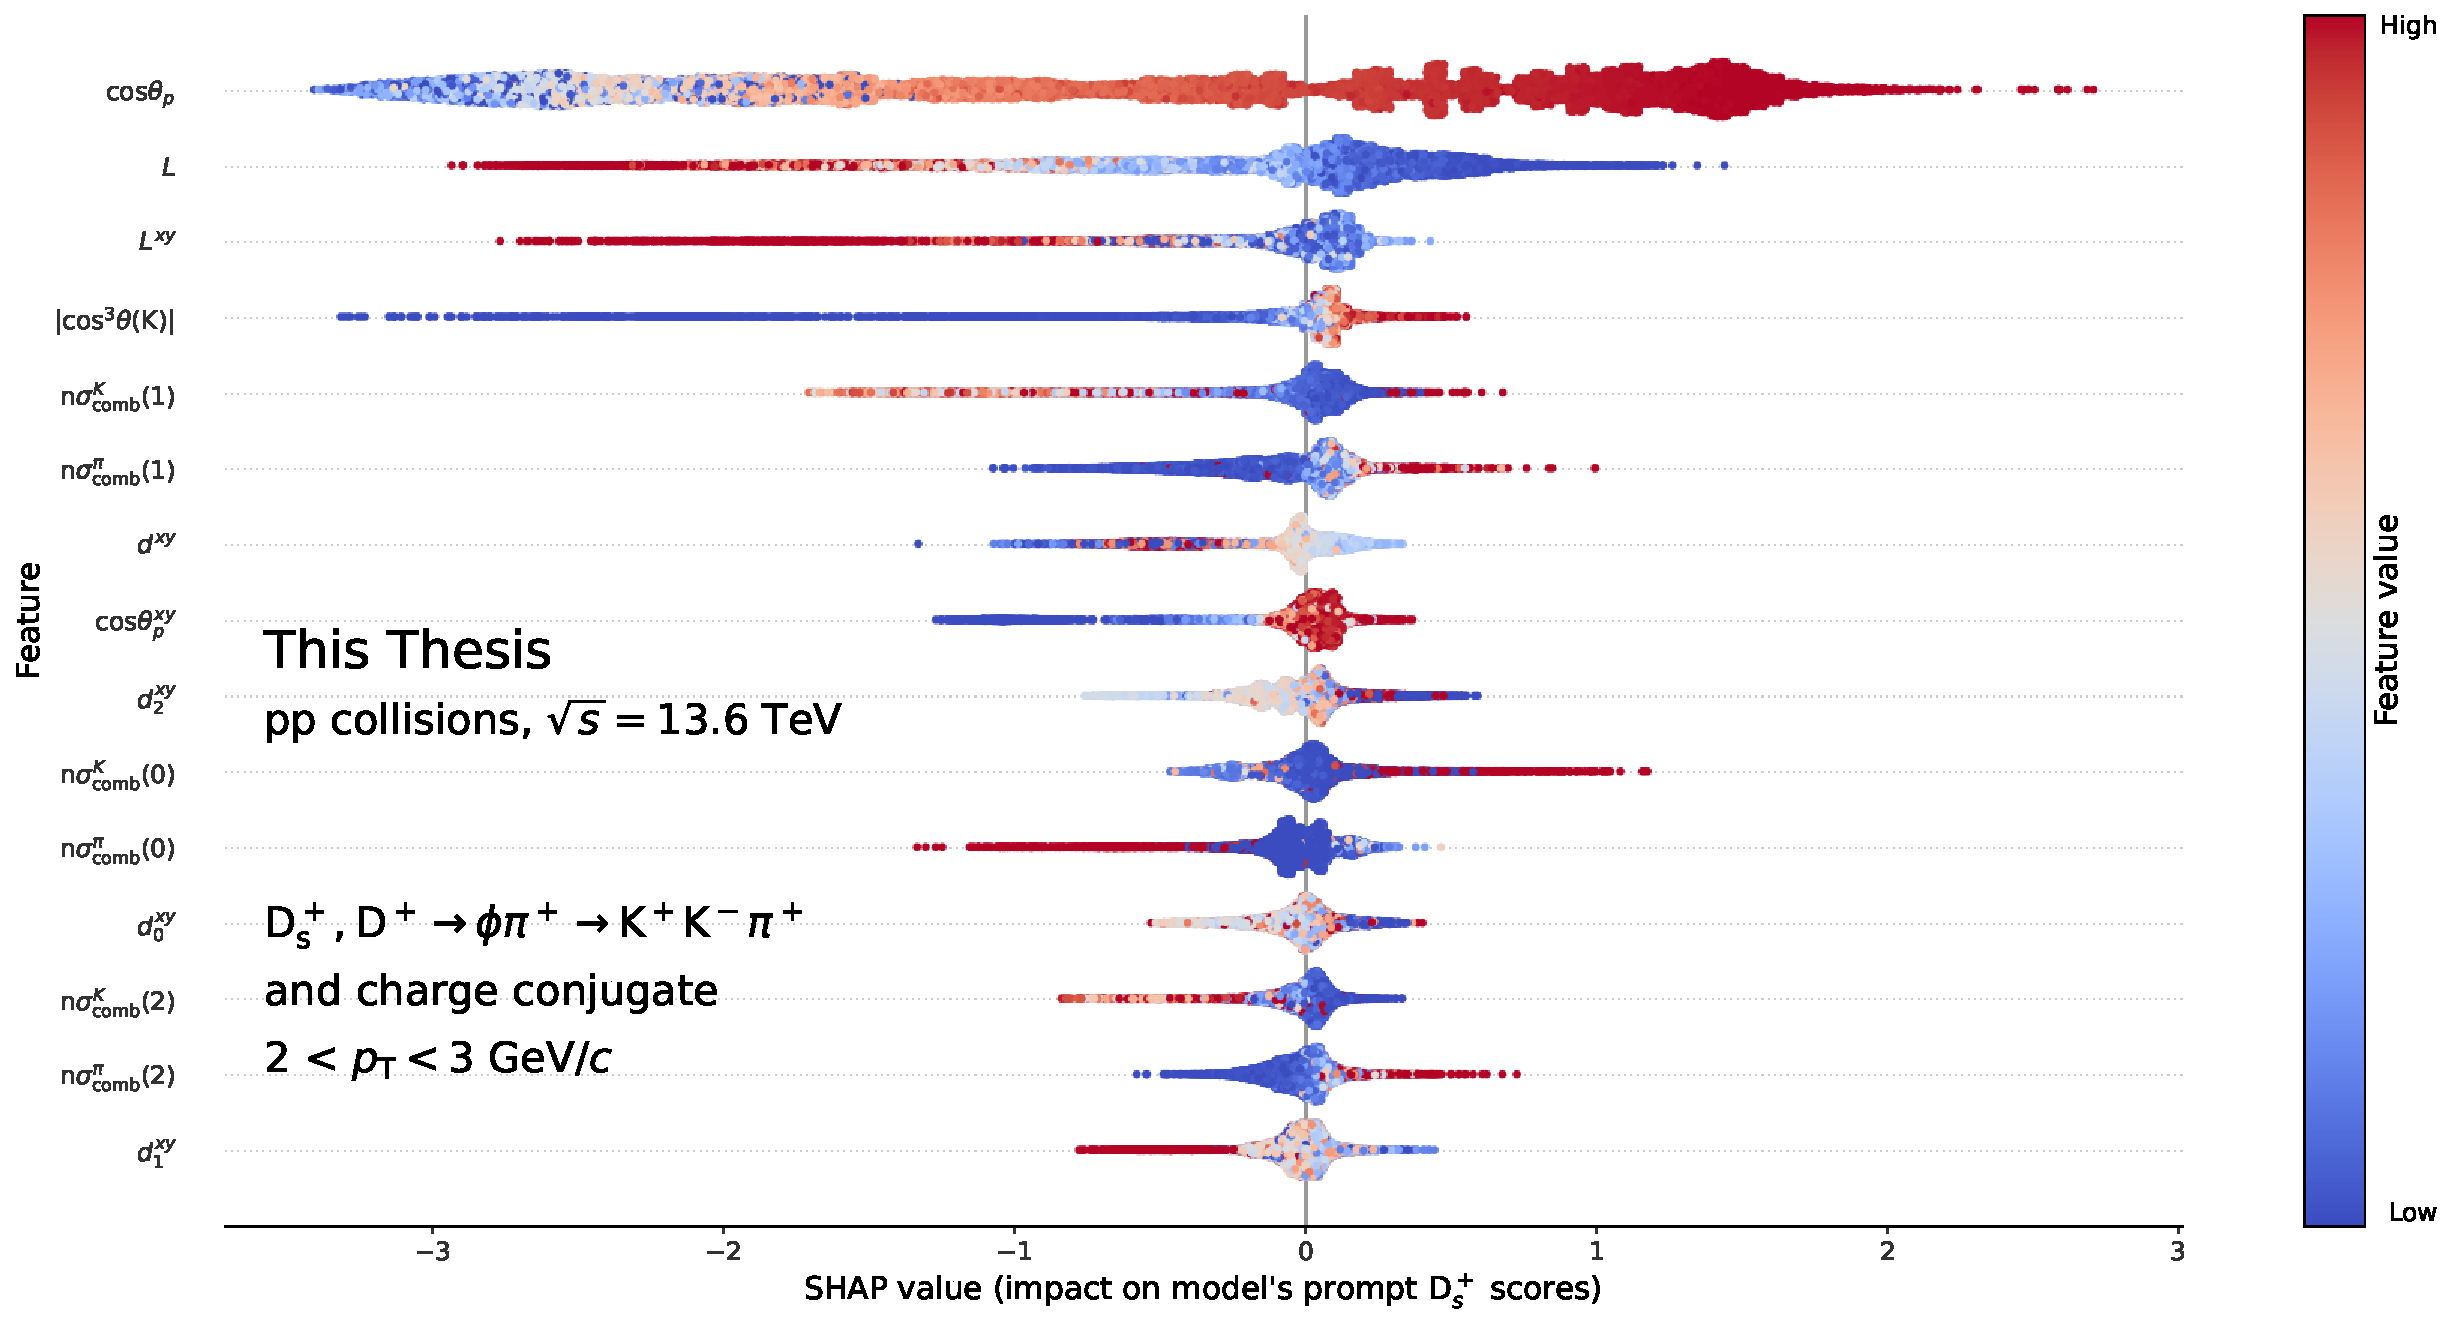
\includegraphics[width=\textwidth]{Figures/Chapter 5/shap.pdf}
    \caption{Beeswarm-style SHAP feature importance plot for the prompt \ds-meson score of the XGBoost model trained on the \mbox{$2<\pt<3$~\gevc} interval.}
    \label{fig:ml_feature_importance}
\end{figure}

For each \pt interval, the SHAP values for the different features employed in the model can be evaluated for the three classes. The overall feature impact on the model's decision can be evaluated by computing the average absolute SHAP value for each feature. The average $|\text{SHAP value}|$ feature importance for the BDT models trained on the $2<\pt<3$~\gevc and $8<\pt<12$~\gevc intervals are shown in Fig.~\ref{fig:ml_feature_importance_average}, providing insights on the evolution of the feature importance across the different \pt intervals. The features are ordered from top to bottom based on their importance, evaluated as the sum of the mean absolute SHAP values for the three classes. Consistently with Fig.~\ref{fig:ml_feature_importance}, in the \mbox{$2<\pt<3$~\gevc} interval the overall most impactful features are the cosine of pointing angle $\cos\theta_\mathrm{p}$, the decay length $L$ and the PID information on the prong 1. Differences in the feature importance order are due to the different importance for the classes other than the prompt \ds meson reported in Fig.~\ref{fig:ml_feature_importance}. In the \mbox{$8<\pt<12$~\gevc} interval, the decay length $L$ and its projection on the transverse plane acquire a significantly higher importance. This is due to the fact that at higher \pt, the decay length of the \ds mesons is larger owing to the higher Lorentz boost, and therefore the selection of both prompt and non-prompt based on their decay length becomes more effective.
\begin{figure}[htb]
    \centering
    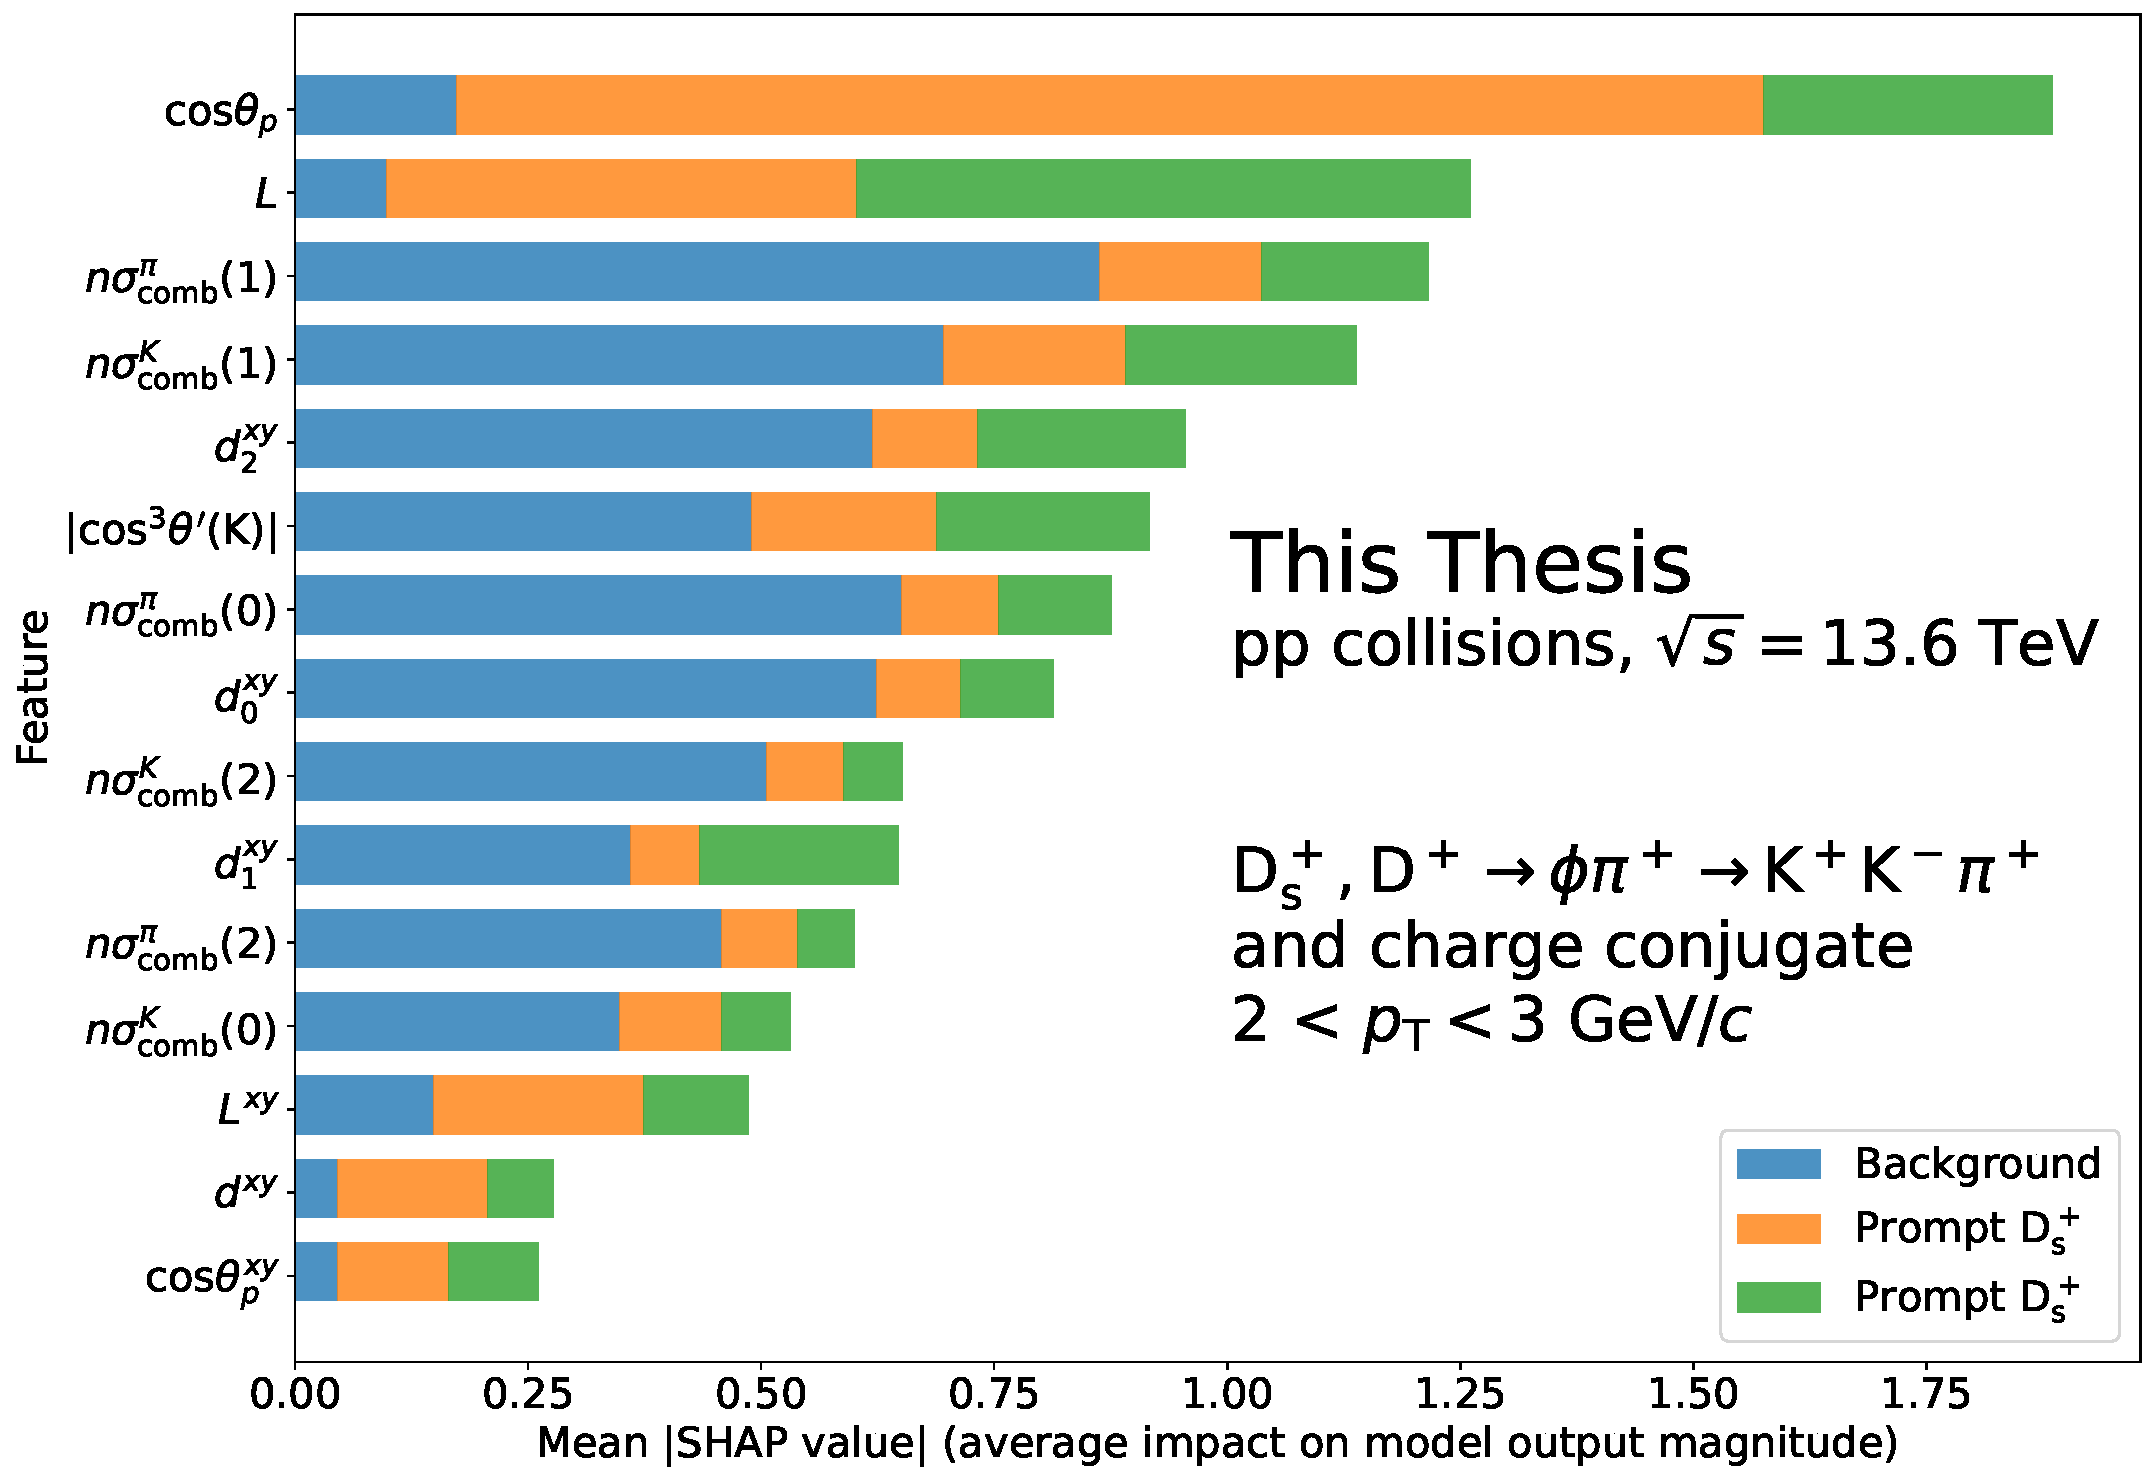
\includegraphics[width=0.48\textwidth]{Figures/Chapter 5/SHAP_summary2_3.pdf}
    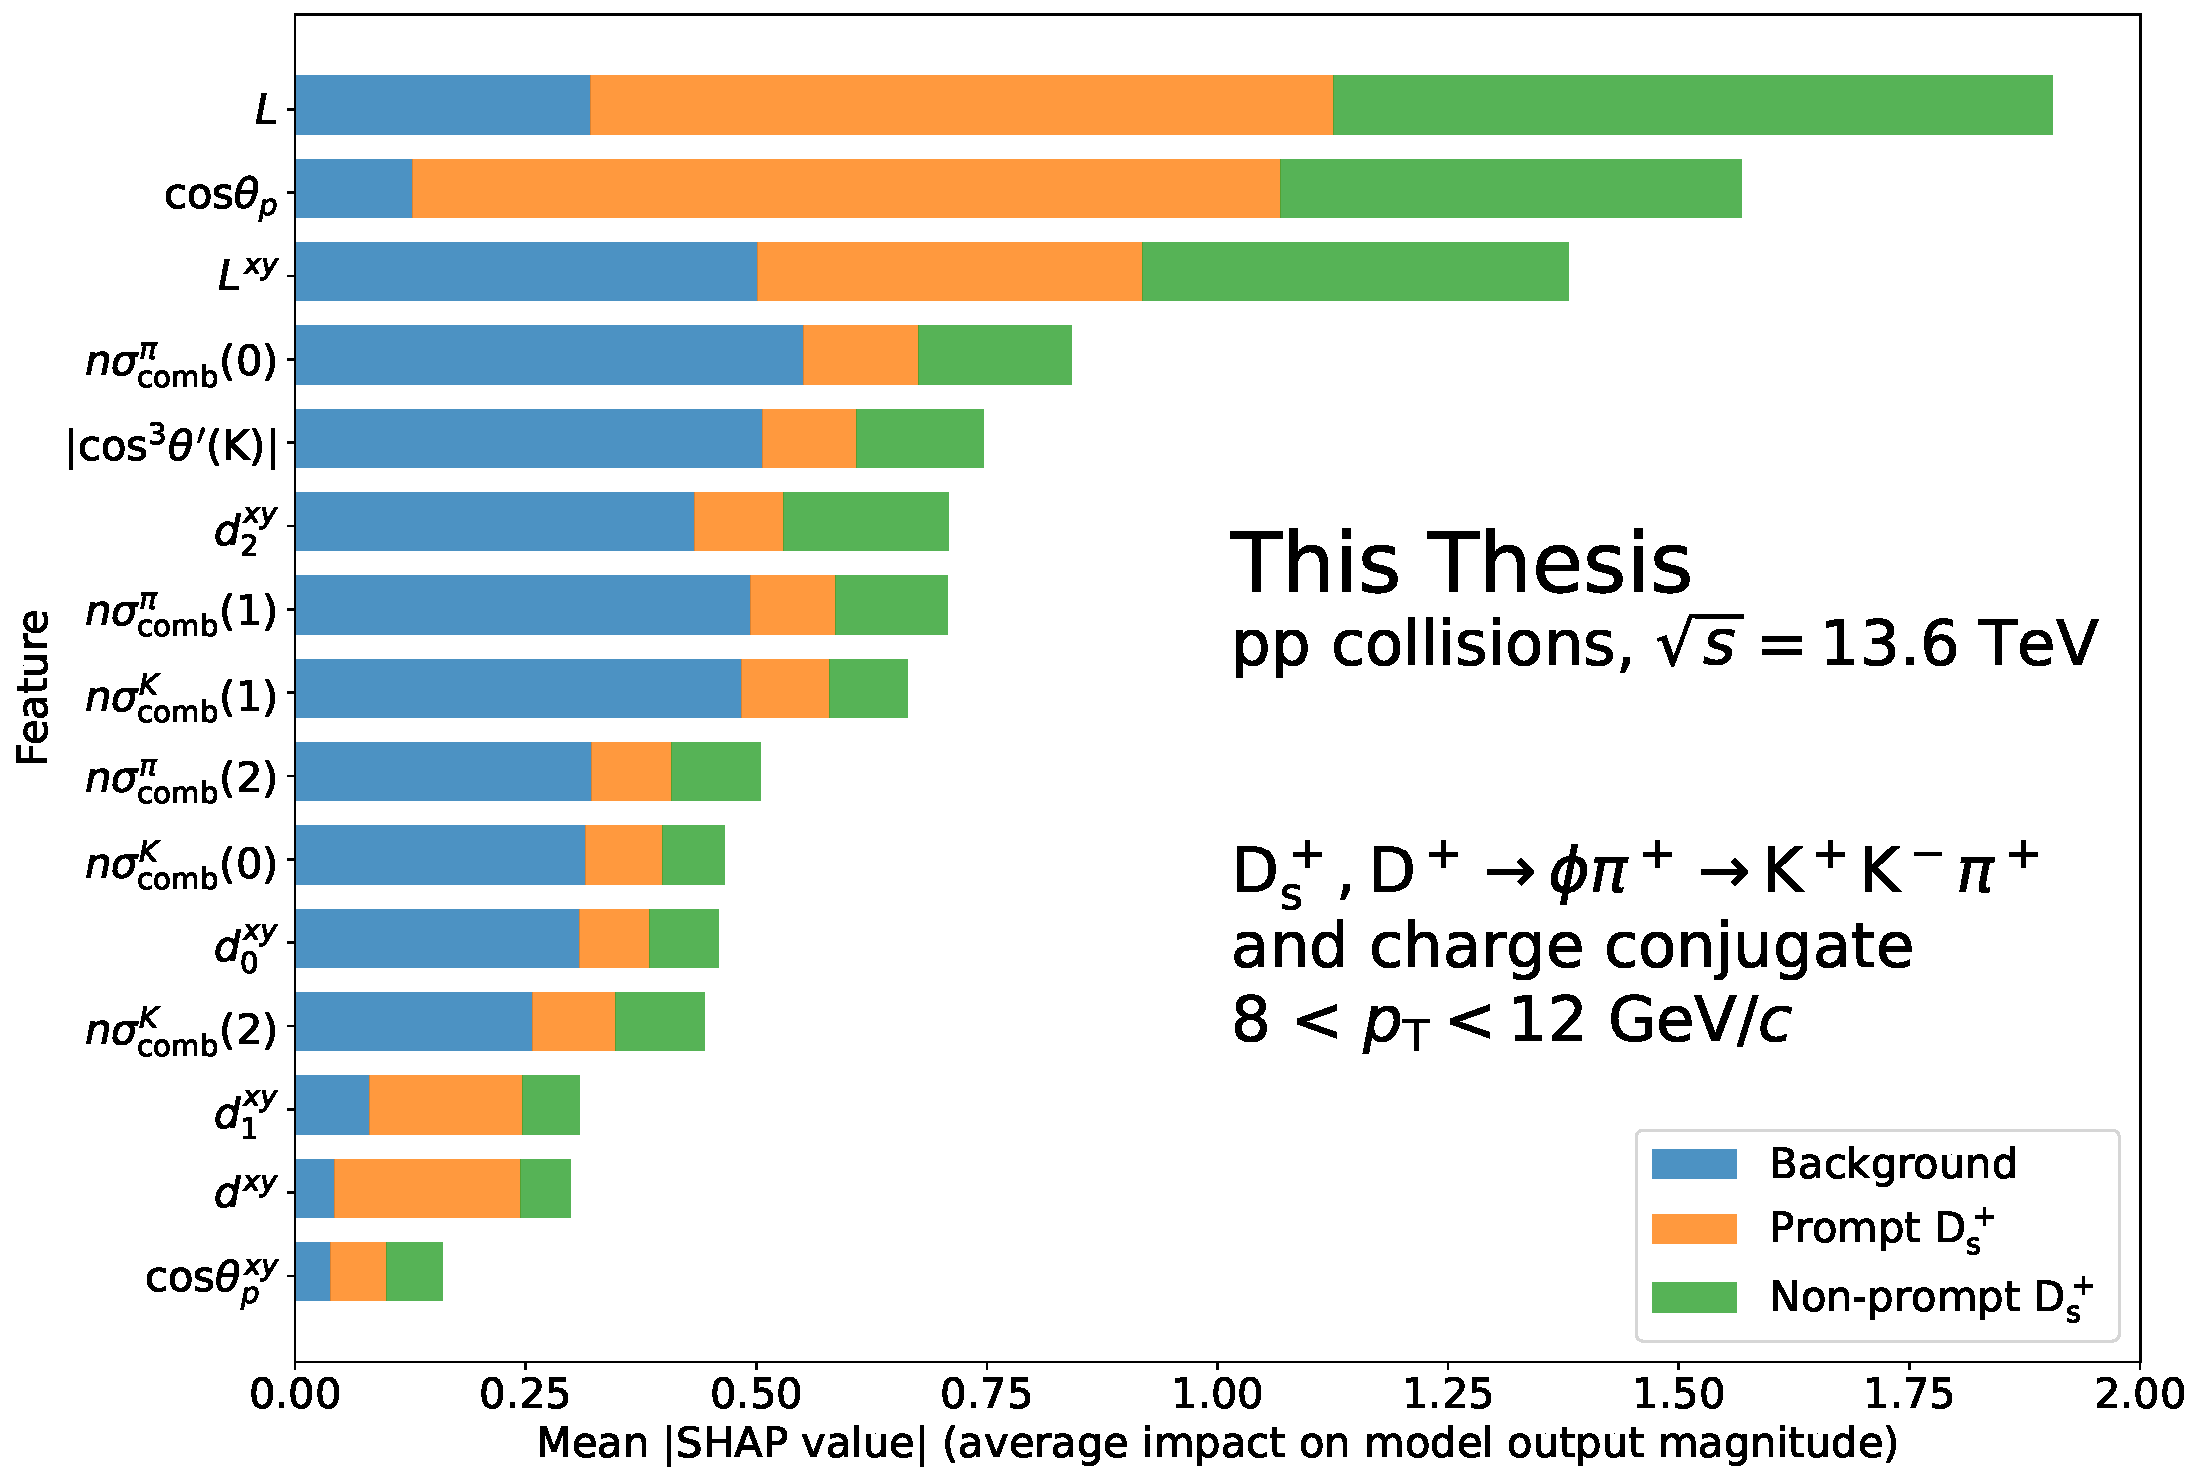
\includegraphics[width=0.48\textwidth]{Figures/Chapter 5/SHAP_summary8_12.pdf}
    \caption{Average $|\text{SHAP value}|$ feature importance for the XGBoost model trained on the \mbox{$2<\pt<3$~\gevc} (left panel) and \mbox{$8<\pt<12$~\gevc} (right panel) intervals. The feature importance for the background, prompt \ds-meson, and non-prompt \ds-meson classes are shown with blue, orange, and green bars, respectively.}
    \label{fig:ml_feature_importance_average}
\end{figure}

\subsection{Optimisation of the selection thresholds on the BDT scores}
Once the model performance has been validated, a set of selection criteria on the BDT output scores has to be chosen to select the candidates. This is a crucial step of the analysis, as it will define the signal selection efficiency and the background contamination. Since the model's output consists of a score related to the probability of belonging to each class, and the three probabilities sum up to unity, the selection criteria have a total of two degrees of freedom. A first selection is applied on the maximum probability to be a background candidate, and rejects most of the contamination from the combinatorial background. The second one is applied on the minimum probability of being a prompt \ds-meson candidate, and suppresses the signal contribution arising from non-prompt \ds-meson candidates. 

A first indication of the optimal selection criteria can be obtained by studying the model's output distributions, e.g., those reported in Fig.~\ref{fig:ml_score}. A good working point can be chosen as the point where a good separation between the three classes is achieved. For this analysis, however, the statistical significance of the extracted inclusive signal (i.e., of both prompt and non-prompt D mesons) is used to define the optimal selection criteria. For each \pt interval of the analysis, the signal $S$ and the background $B$ are evaluated by fitting the invariant mass distribution of candidates from the data passing the different ML selections considered in the optimisation process. Only a subset of the full dataset, corresponding to approximately 3\% of the available data sample is used in this process. The working point is chosen using different considerations. Firstly, the selection criteria are chosen to maximise the statistical significance of the signal, defined as $S/\sqrt{S+B}$. This definition of statistical significance is equivalent to the inverse of the relative statistical uncertainty on the signal, for a Poisson distribution of candidate counts. Thus, maximising the statistical significance corresponds to minimising the relative statistical uncertainty on the signal. In order to avoid an over-optimisation of the model to enhance the statistical significance (which could bias the results if statistical fluctuations are not properly taken into account), the considered threshold values on the BDT output scores are multiples of 0.05. Additionally, the efficiency of the selection is checked to ensure that it is kept at sufficiently high levels, to reduce possible biases in the final results due to possible imperfections in the MC description of the data. A smooth increasing trend with \pt of the efficiency is also ensured to provide consistency in the tightness of the selection criteria across the different \pt intervals. 

Usually, the maximisation of the statistical significance is avoided in the choice of the selection criteria, as it can lead to a bias in the final results. However, in this case, the optimisation is performed on a very small fraction of the data thanks to the large dataset available, and the bias is expected to be negligible. A different approach to select an optimal working point consists in the optimisation of a pseudo-significance, defined as the ratio of the expected signal and the square root of the sum of the expected signal and the expected background. For each considered selection criterion, the selection efficiency is evaluated on MC simulations, and the expected signal is estimated from the D-meson production cross section provided by FONLL~\cite{Cacciari:1998it} theoretical predictions. The expected background is estimated from a fit of the invariant mass distribution of the candidates in the sidebands of the signal region. This approach avoids the introduction of a bias in the final results, as it is blind to the candidates in the signal region. However, it relies on FONLL predictions and MC simulations. To avoid the introduction of biases in the optimisation due to shortcomings of FONLL predictions or MC simulations, the optimisation of the pseudo-significance is not performed in this analysis.

A result of the working point optimisation is presented in Fig.~\ref{fig:ml_significance} for the \mbox{$2.0<\pt<2.5$~\gevc} interval. The statistical significance of the signal is shown as a function of the BDT output score threshold for the probability of being a prompt \ds meson and a background candidate. The chosen set of selection criteria is shown with a green cross.

The optimal selection criteria for each \pt interval considered in the analysis are reported in Table~\ref{tab:working_point}. Because of the large combinatorial background and the small Lorentz boost of the \ds mesons, which results in a small decay length and a less effective selection based on the displaced topology, the selection criteria in the lowest \pt intervals are chosen to be stringent to extract the signal with a large enough signal-to-background ratio. At higher \pt, the selection criteria are loosened, as the larger decay length of the \ds mesons results in a more effective separation between signal and background candidates. In addition, at higher \pt the combinatorial background is reduced, and the selection criteria can be loosened to increase the signal efficiency. The threshold on the prompt \ds-meson probability is kept at around 0.2 for all \pt intervals. This selection allows a significant reduction of the contamination from non-prompt D mesons in the selected sample, while it does not considerably influence the statistical significance of the signal. In the \mbox{$5.5<\pt<6.0$~\gevc} interval, the threshold is increased to 0.25 to guarantee an increasing trend of the efficiency with \pt.

\begin{figure}
    \centering
    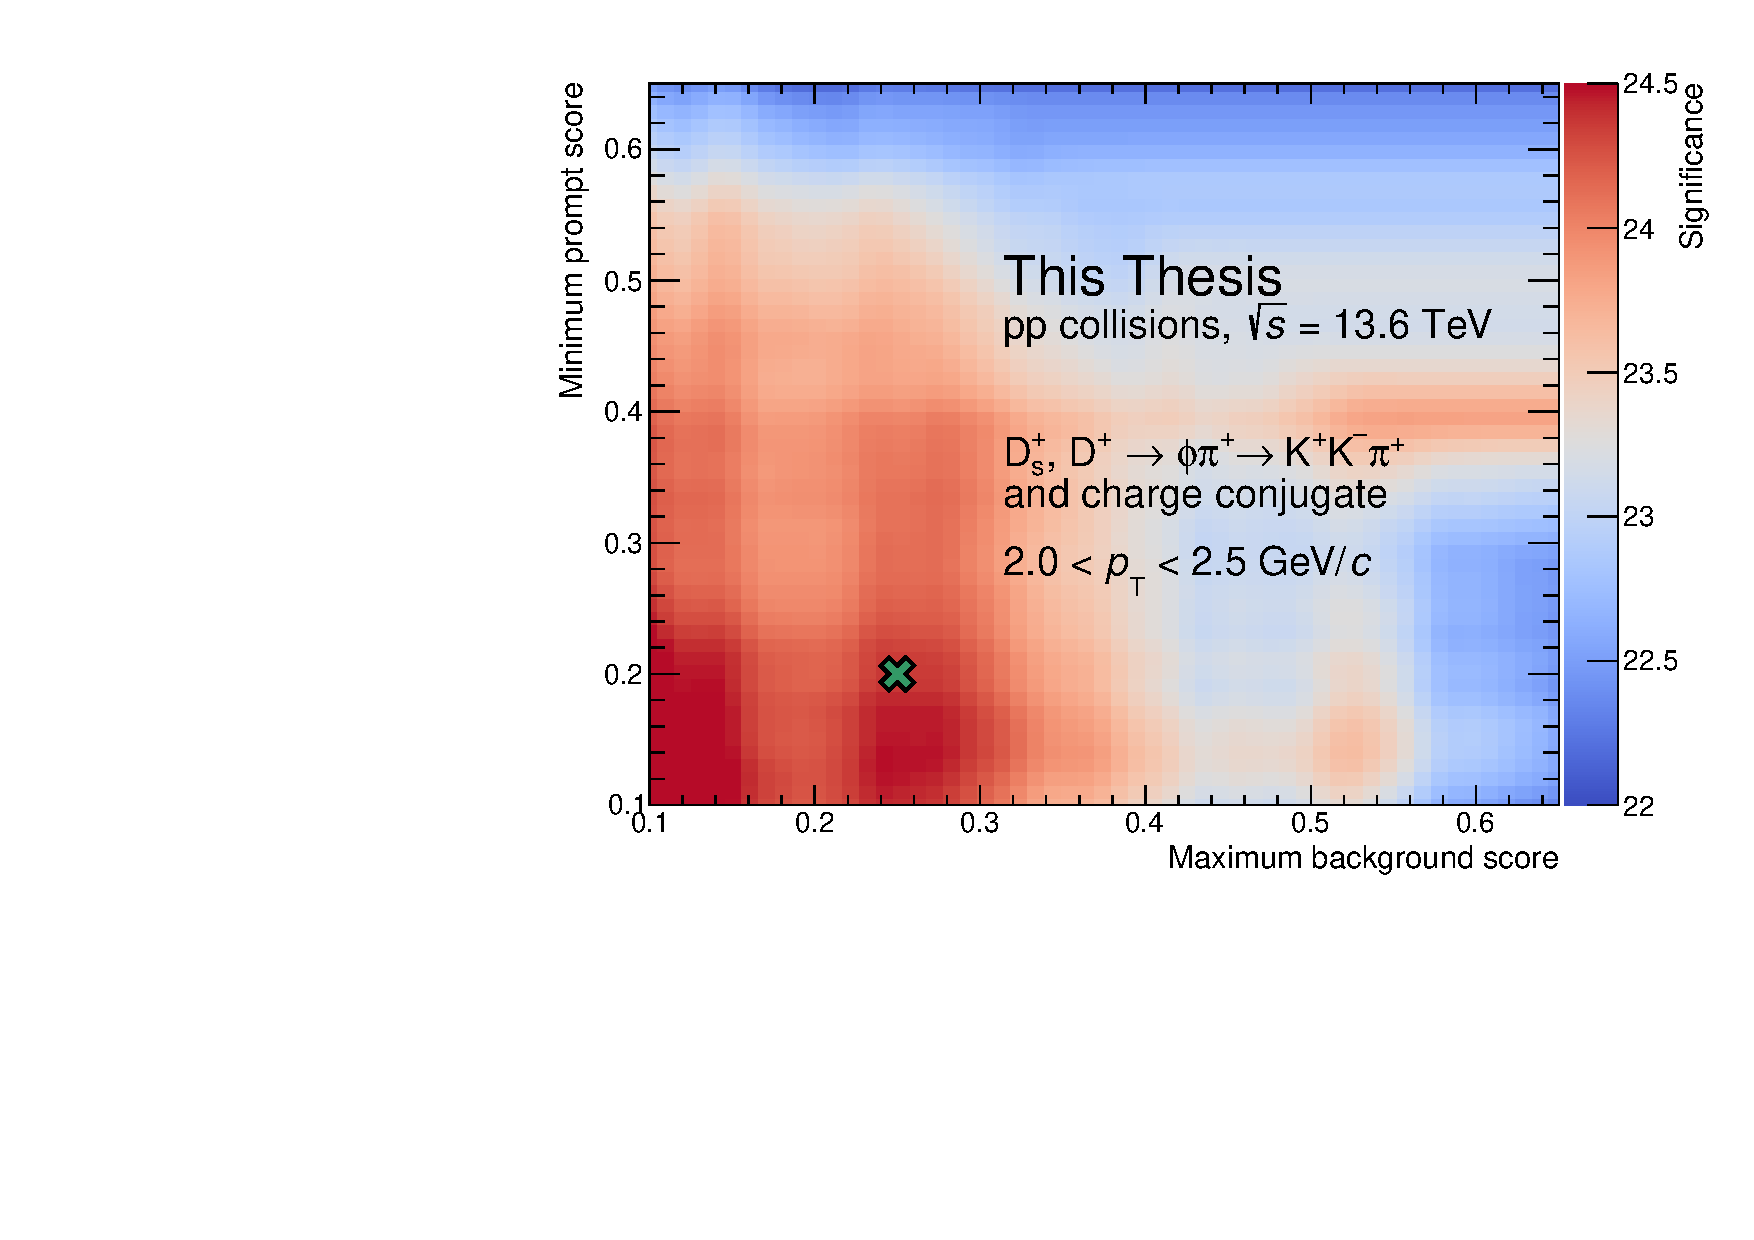
\includegraphics[width=0.7\textwidth]{Figures/Chapter 5/Significance_Scan_2_2p5.pdf}
    \caption{Statistical significance of the signal as a function of the selection criteria applied to the model output for the $2.0<\pt<2.5$~\gevc interval. The chosen set of selection criteria is shown with a green cross.}
    \label{fig:ml_significance}
\end{figure}

\begin{table}[b!]
    \centering
    \caption{Selection criteria applied to enhance the significance of the $\ds$ meson signal in the $\pt$ intervals considered for the analysis.}
    \label{tab:working_point}
    \vspace*{0.3cm}
    \resizebox{\columnwidth}{!}{%
    \begin{tabular}{c|cc}
    \toprule
         \pt interval (\gevc) & Probability to be background $<$ & Probability to be prompt \ds meson $>$  \\
         \midrule
         0.5$-$1.0 & 0.01 & 0.20 \\
         1.0$-$1.5 & 0.05 & 0.20 \\
         1.5$-$2.0 & 0.15 & 0.20 \\
         2.0$-$2.5 & 0.25 & 0.20 \\
         2.5$-$3.0 & 0.30 & 0.20 \\
         3.0$-$3.5 & 0.20 & 0.20 \\
         3.5$-$4.0 & 0.20 & 0.20 \\
         4.0$-$4.5 & 0.20 & 0.20 \\
         4.5$-$5.0 & 0.20 & 0.20 \\
         5.0$-$5.5 & 0.30 & 0.20 \\
         5.5$-$6.0 & 0.30 & 0.25 \\
         6$-$8   & 0.45 & 0.20 \\
         8$-$12  & 0.50 & 0.20 \\
         12$-$24 & 0.55 & 0.20 \\
        \bottomrule
    \end{tabular}%
    }
\end{table}

\section{\texorpdfstring{\ds and \dpl raw-yield extraction}{Ds+ and D+ mesons raw-yield extraction}}

After the working point for the BDT algorithm has been defined, the raw yields of \ds and \dpl mesons are extracted in each \pt interval. They are defined as the sum of particles and antiparticles and are measured in 14 \pt intervals in the range $0.5<\pt<24$~\gevc. The raw yield is extracted by fitting the invariant mass distribution of the selected candidates. 

In several analyses performed by the ALICE Collaboration during the Run~2 data-taking period~\cite{ALICE:2021mgk,ALICE:2023sgl,ALICE:2021kfc}, the raw yield of \ds mesons was extracted by fitting the invariant mass distribution of selected candidates with a probability density function constructed as the sum of a function describing the shape of the combinatorial background (usually an exponential function or a low-order ($<3$) polynomial) and of two Gaussian distributions to model the \ds- and \dpl-meson peaks. The raw yields for the two D-meson species are then obtained by integrating the signal function. 

Figure~\ref{fig:old_fit} shows the fit to the invariant mass distribution of the selected candidates in the \mbox{$1.5<\pt<2.0$~\gevc} interval using the approach described above. Due to the concavity-changing shape of the background, the function chosen to describe the background is a third-order polynomial. This change in the concavity of the background invariant-mass distribution was not observed in previous analyses performed on pp collisions data collected during the LHC Run~2 data-taking period. With the upgrade of the ALICE experimental apparatus, the amount of data collected during the ongoing LHC Run~3 data-taking period is significantly larger than that collected during Run~2, as described in Chapter~\ref{chap:ALICE}. With the increased number of candidates available, the statistical precision of the data sample is higher, and the concavity-changing shape of the background becomes more evident. The small number of candidates available in the Run~2 data sample did not allow for the observation of this feature, as statistical uncertainties covered the shape of the background. On top of the previously-unobserved peculiar shape of the background, the fitting function is not able to describe the data accurately between the two peaks, overestimating the data in this invariant mass region.

\begin{figure}[htb]
    \centering
    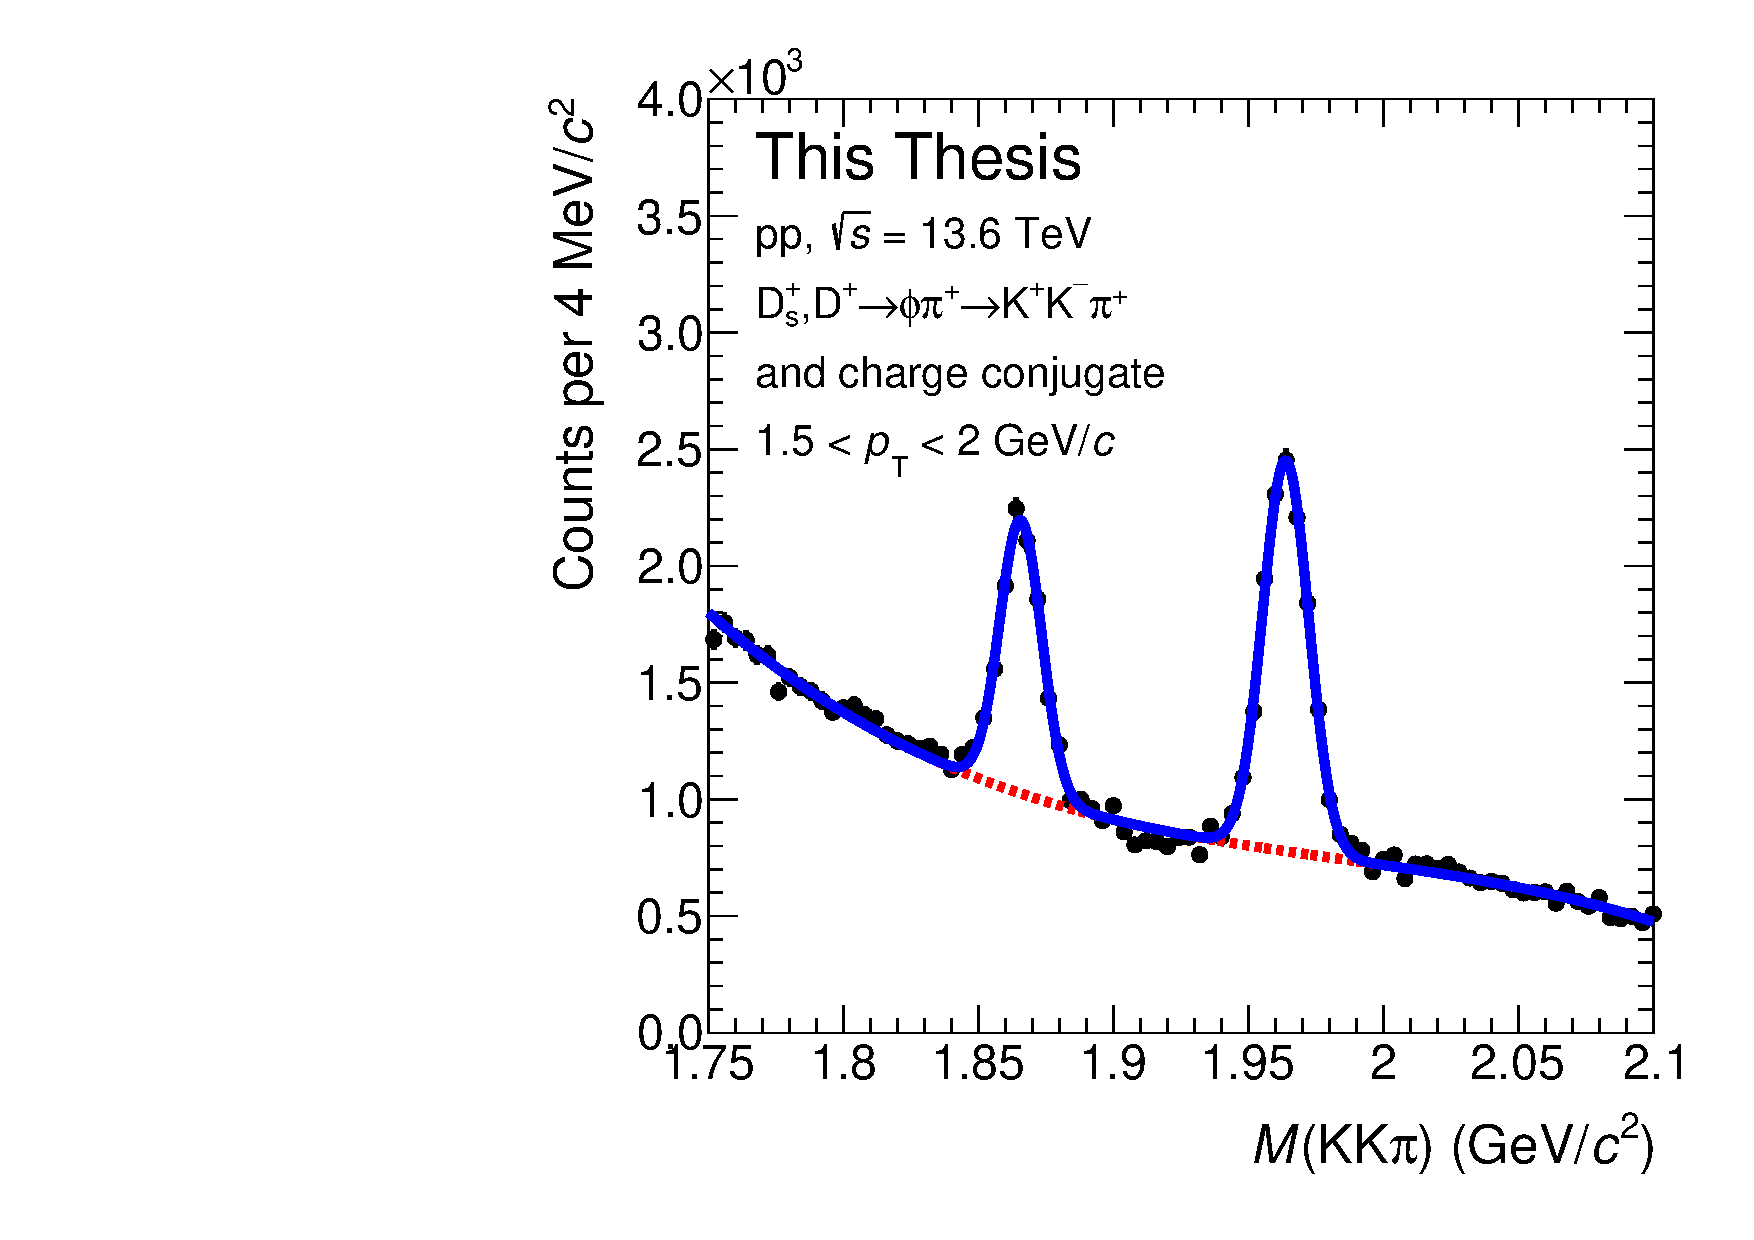
\includegraphics[width=0.7\textwidth]{Figures/Chapter 5/InvMassFitDs1p5_2.pdf}
    \caption{Fit to the invariant mass distribution of selected candidates in the \mbox{$1.5<\pt<2.0$~\gevc} interval. The fit function is shown as a solid line, while the signal and background components are shown as dashed lines. The background is modelled with a third-order polynomial function.}
    \label{fig:old_fit}
\end{figure}

These two features can be understood as due to the fact that the background does not solely arise from the combination of independent tracks, i.e., the combinatorial background. Other physics processes can contribute to the contamination of the data sample, giving rise to a \emph{correlated background}. One such process is the decay of \dpl mesons into the $\dpl\rightarrow\mathrm{\pi^+K^-\pi^+}$ decay channel, where one of the pions is misidentified as a kaon. Despite being suppressed by the applied PID and ML selections, this contribution can give rise to a noticeable contribution due to the large BR of $9.38\%$~\cite{pdg}.

\begin{sloppypar}
To validate this hypothesis, a simulation of \dpl-meson decays into \mbox{$\dpl\rightarrow\mathrm{\pi^+K^-\pi^+}$} was run using \textsc{Pythia}~8~\cite{Bierlich:2022pfr}. Ten billion \dpl mesons were produced with a uniformly distributed \pt spectrum in the $0<\pt<24$~\gevc interval. The \dpl mesons were then forced to decay into the $\dpl\rightarrow\mathrm{\pi^+K^-\pi^+}$ decay channel. For each decay, two invariant masses were evaluated, by assigning the kaon mass to one of the two pions to simulate the misidentification of one pion, while the correct masses were assigned to the other two prongs. The invariant mass distributions obtained from the simulation are shown in Fig.~\ref{fig:DplusSimulations} for different \pt intervals. The distribution is characterised by a peak at $\sim 2$~\gevcc, well inside the fit range used to extract the raw yield of \ds and \dpl mesons in Fig~\ref{fig:old_fit}. In addition, the invariant mass distribution evolves with the \pt of the \dpl meson, with a tail towards higher invariant masses for higher \pt values. This follows naturally from the kinematic properties of the decay. Other sources of correlated background can be present (e.g., from \lc decays), but their contribution was found to be negligible.
\end{sloppypar}

\begin{figure}[htbp]
    \centering
    \includegraphics[width=\textwidth]{Figures/Chapter 5/Dplus_Corr_Bkg_simulation.pdf}
    \caption{Invariant-mass distribution of simulated decays of \dpl mesons into \mbox{$\dpl\rightarrow\mathrm{\pi^+K^-\pi^+}$}, where one of the pions produced in the decay is misidentified as a kaon. Distributions for different \pt intervals are shown. }
    \label{fig:DplusSimulations}
\end{figure}

To account for this contribution, a template contribution is included in the fit function, in addition to the combinatorial background and the two signal peaks. This method involves fitting the invariant mass distribution using a predefined template to model the misidentified $\dpl\rightarrow\mathrm{\pi^+K^-\pi^+}$ decay, whose shape is fixed, and the only adjustable parameter is the normalisation. The shape of the template is taken from the same simulation used to train the BDT model, as described in Sec.~\ref{sec:ml_data_preparation}, where $\dpl\rightarrow\mathrm{\pi^+K^-\pi^+}$ mesons reconstructed as $\dpl\rightarrow\mathrm{K^+K^-\pi^+}$, passing PID selections as $\mathrm{K^+K^-\pi^+}$, are selected. The distribution is fixed to that obtained before applying any ML model, as it was studied that the applied ML selections do not affect the shape of the correlated background. This allows for reducing statistical fluctuations in the template shape. The final fit function is then constructed as the sum of a parabolic function to describe the combinatorial background, the template function described above for the correlated $\dpl\rightarrow\mathrm{\pi^+K^-\pi^+}$ background source, and two Gaussian functions to describe the \ds- and \dpl-meson peaks. The signal parameters (mean, width, normalisation), as well as the parameters of the combinatorial background and the normalisation of the template fit are left free in the fit in the \pt intervals below 8~\gevc. Because of the observed momentum resolution worsening at higher \pt, and because of the smaller number of candidates available in the high-\pt intervals, for the $\pt>8$~\gevc range the widths of the \dpl-meson signal peaks are fixed to those of the \ds meson divided by a factor 1.2, which is the observed ratio of the peak widths at low \pt, with a flat trend with \pt, as illustrated in Fig.~\ref{fig:sigma_ratio}. In the left panel, the evolution of the peak widths of the \ds and \dpl mesons as a function of \pt is shown for both data and MC simulations. A clear increasing trend of the peak widths with \pt is observed because of the degrading momentum resolution due to the decreasing track curvature. MC simulations underestimate the peak widths extracted from the data for both \ds and \dpl mesons, across the studied \pt range. In the right panel of Fig.~\ref{fig:sigma_ratio}, the ratio between the peak widths of the \ds and \dpl mesons is shown as a function of \pt, for both data and MC simulations. The ratio is observed to be almost constant across the analysed \pt range, with a value of $\sim 1.2$. The ratio is underestimated by the MC simulations, which predict a value of $\sim 1.1$ across the studied \pt range.

In the \pt interval above 8~\gevc, where the peak width of the \dpl meson is fixed to that of the \ds meson divided by a factor of 1.2, a first fit is performed by keeping both peak widths as free parameters. Then, the \dpl-meson peak width is fixed to that of the \ds divided by 1.2, and the fit is repeated, keeping the remaining parameters free. Additionally, in order to correctly describe the background shape, the fit is performed in the invariant mass range \mbox{$1.73<M(\mathrm{KK\pi})<2.15$~\gevcc} for \mbox{$\pt>5$~\gevc}, while a narrower invariant mass window, \mbox{$1.75<M(\mathrm{KK\pi})<2.1$~\gevcc}, is used at lower \pt. The invariant-mass bin width has been fixed to 2~\mevcc. The fits to the invariant mass distributions of selected D-meson candidates are performed using the \code{flarefly} package~\cite{grosa_2023_7579657}, which provides a flexible Python interface for performing fits. 

\begin{figure}[htb]
    \centering
    \includegraphics[width=0.48\textwidth]{Figures/Chapter 5/SigmaDs_Dplus.pdf}
    \includegraphics[width=0.48\textwidth]{Figures/Chapter 5/SigmaDsOverDplusMC.pdf}
    \caption{Left panel: peak width of the \ds and \dpl mesons as a function of \pt, before fixing the width of the \dpl meson to that of the \ds meson divided by a factor of 1.2 for $\pt>8~\gevc$. Both the peak widths from fits to data and MC simulations are reported. Right panel: ratio of the peak widths of the \ds and \dpl mesons as a function of \pt, for both data and MC simulations.}
    \label{fig:sigma_ratio}
\end{figure}


The fit to the invariant mass distribution of candidates passing the ML selections is shown in Fig.~\ref{fig:new_fit} for one representative \pt interval of $2.0<\pt<2.5$~\gevc. The total fit function is shown as a solid blue line, the signal contributions are shown as filled green and azure areas for \dpl and \ds mesons, respectively, the combinatorial background is represented with a solid red line, while the correlated background is shown as a dashed violet line. The fit is able to describe the data accurately, as can be deduced from the distribution of the difference between the data and the background fit function, shown in the bottom panels for the two \pt bins. 

\begin{figure}[htb]
    \centering
    \includegraphics[width=0.7\textwidth]{Figures/Chapter 5/invmassfit_2_2p5.pdf}
    \caption{Fit to the invariant mass distribution of selected candidate in the \mbox{$2.0<\pt<2.5$~\gevc} interval. The total fit function is shown as a solid blue line, while background components are shown as solid red lines (correlated background) and dashed violet lines (dashed violet lines). The signal contributions are shown as filled green and azure areas for \dpl and \ds mesons, respectively. The bottom panels show the distribution of the difference between the data and the background fit function.}
    \label{fig:new_fit}
\end{figure}

The complete set of fits to the invariant mass distributions in the 14 studied \pt intervals is shown in Fig.~\ref{fig:new_fit_all}. All the fits present a good level of agreement between the data and the fit function. Figure~\ref{fig:new_fit_all} also shows that the contribution of the correlated $\dpl\rightarrow\mathrm{\pi^+K^-\pi^+}$ background evolves with \pt, with a larger contribution at lower \pt values. The raw yield of \ds and \dpl mesons is then extracted by integrating the signal function.

\begin{sidewaysfigure}[p]
    \centering
    \includegraphics[width=0.2\textwidth]{Figures/Chapter 5/inv_mass/pt_0.5_1.0.pdf}
    \includegraphics[width=0.2\textwidth]{Figures/Chapter 5/inv_mass/pt_1.0_1.5.pdf}
    \includegraphics[width=0.2\textwidth]{Figures/Chapter 5/inv_mass/pt_1.5_2.0.pdf}
    \includegraphics[width=0.2\textwidth]{Figures/Chapter 5/inv_mass/pt_2.0_2.5.pdf}
    \includegraphics[width=0.2\textwidth]{Figures/Chapter 5/inv_mass/pt_2.5_3.0.pdf}
    \includegraphics[width=0.2\textwidth]{Figures/Chapter 5/inv_mass/pt_3.0_3.5.pdf}
    \includegraphics[width=0.2\textwidth]{Figures/Chapter 5/inv_mass/pt_3.5_4.0.pdf}
    \includegraphics[width=0.2\textwidth]{Figures/Chapter 5/inv_mass/pt_4.0_4.5.pdf}
    \includegraphics[width=0.2\textwidth]{Figures/Chapter 5/inv_mass/pt_4.5_5.0.pdf}
    \includegraphics[width=0.2\textwidth]{Figures/Chapter 5/inv_mass/pt_5.0_5.5.pdf}
    \includegraphics[width=0.2\textwidth]{Figures/Chapter 5/inv_mass/pt_5.5_6.0.pdf}
    \includegraphics[width=0.2\textwidth]{Figures/Chapter 5/inv_mass/pt_6.0_8.0.pdf}
    \includegraphics[width=0.2\textwidth]{Figures/Chapter 5/inv_mass/pt_8.0_12.0.pdf}
    \includegraphics[width=0.2\textwidth]{Figures/Chapter 5/inv_mass/pt_12.0_24.0.pdf}
    \caption{Fit to the invariant mass distribution of selected candidate in the 14 studied \pt intervals in the \mbox{$0.5<\pt<24$~\gevc} range. The total fit function is shown as a solid blue line, while background components are shown as solid red lines (correlated background) and dashed violet lines (dashed violet lines). The signal contributions are shown as filled green and azure areas for \dpl and \ds mesons, respectively.}
    \label{fig:new_fit_all}
\end{sidewaysfigure}

The evolution of the mean and width of the \ds and \dpl meson peaks as a function of \pt is shown in Fig.~\ref{fig:mean_width}. In the left panel, the means of the Gaussian functions used to describe the \ds- and \dpl-meson peaks are shown as a function of \pt. They present an increasing trend with \pt lying below the values reported in the PDG~\cite{pdg}, represented with dashed lines. The shift of the mass values observed in data from those reported in the PDG is common to all analyses of D mesons due to an imperfect description of the detector misalignments in MC simulations. In the right panel, the peak widths of the \ds and \dpl mesons, defined as the standard deviation of the Gaussian functions used to describe their invariant mass distributions, are shown as a function of \pt. An increasing trend with \pt is observed for both mesons, as detailed above for Fig.~\ref{fig:sigma_ratio}, with the peak width of the \ds meson being larger than that of the \dpl meson across the studied \pt range.

\begin{figure}[htb]
    \centering
    \includegraphics[width=0.48\textwidth]{Figures/Chapter 5/Mean.pdf}
    \includegraphics[width=0.48\textwidth]{Figures/Chapter 5/Sigma.pdf}
    \caption{Evolution of the mean (left panel) and width (right panel) of the Gaussian functions used to describe the \ds and \dpl meson peaks as a function of \pt. The dashed lines in the left panel represent the mass values reported in the PDG~\cite{pdg} for the two D-meson species.}
    \label{fig:mean_width}
\end{figure}

The relative contribution of the $\dpl\rightarrow\mathrm{\pi^+K^-\pi^+}$ correlated background to the total fitting function is shown in the left panel of Fig.~\ref{fig:frac_signif} as a function of \pt. At low \pt, where the PID is more effective, the contribution of the correlated background is observed to be smaller. It then increases up to 2~\gevc and then decreases due to the kinematic properties of the decay as expected from Fig.~\ref{fig:DplusSimulations}. Some residual contribution is observed at higher \pt, related to fluctuations in the fitting procedure. In the right panel of Fig.~\ref{fig:frac_signif}, the statistical significance of the extracted \ds- and \dpl-meson signals is shown as a function of \pt. Due to the large combinatorial background at low \pt, the statistical significance presents a decreasing trend with decreasing \pt for $\pt\lesssim2$~\gevc, for both D mesons. The maximum statistical significance is observed in the $2.5<\pt<3.0$~\gevc interval for the \ds meson and in the $2.0<\pt<2.5$~\gevc range for the \dpl meson, where significances of 99 and 50 are reached for the two meson species, respectively. At higher \pt, the statistical significance decreases due to the smaller number of produced D mesons, and the larger peak widths of the \ds and \dpl mesons, which result in a larger background contribution in the signal region. A sudden increase in the statistical significance is observed in the $6<\pt<8$~\gevc interval, and is due to an increase of the width of the \pt interval for the signal extraction, from 0.5~\gevc to 2~\gevc, which results in a larger number of candidates available in the signal region.

\begin{figure}[htb]
    \centering
    \includegraphics[width=0.48\textwidth]{Figures/Chapter 5/Frac.pdf}
    \includegraphics[width=0.48\textwidth]{Figures/Chapter 5/Significance.pdf}
    \caption{Evolution of the $\dpl \rightarrow \mathrm{\pi^+K^-\pi^+}$ relative contribution to the fitting function (left panel) and statistical significance of the extracted \ds- and \dpl-meson signal (right panel) as a function of \pt.}
    \label{fig:frac_signif}
\end{figure}



The extraction of the raw yields is affected by several arbitrary choices, for example, the functional description of the background, the choice of the fit range, the choice of fixing the \dpl width at high \pt, and the invariant-mass bin width. Changes in these choices can lead to variations in the extracted raw yields. To estimate the effect of such arbitrary choices in the final observable (the \ds/\dpl production-yield ratio), and estimate a systematic uncertainty associated with the raw yield extraction procedure, the fit is repeated several times by varying the fit range, the bin width, and the functional form of the background. In the low \pt region ($\pt<4~\gevc$), the lower fit limit is varied between 1.71 and 1.77~\gevcc, while the upper limit is varied between 2.08 and 2.14~\gevcc. The functions considered to describe the background are a second-order polynomial and an exponential function. At higher \pt (up to 8~\gevc), where the signal peaks become broader, the lower limit is varied between 1.71 and 1.75~\gevcc, while the maximum mass is varied between 2.13 and 2.19~\gevcc. The functions considered to describe the background are a second- and a third-order polynomial, as the exponential function was observed not to reproduce the background distribution. The bin width is varied between 1 and 4~\mevcc across the studied \pt interval. At $\pt>8$~\gevcc, where the \dpl-meson peak width is fixed to that of the \ds-meson divided by 1.2, the peak width of the \dpl meson is changed by varying the dividing factor by $\pm10\%$. For each possible combination of these variations, the signal is extracted for the two D-meson species, and the ratio between them is calculated. This results in 128, 96, and 288 trials for the $0.5<\pt<4$~\gevc, $4<\pt<8$~\gevc, and $8<\pt<24$~\gevc intervals, respectively. As a quality check, trials with a $\chi^2/\mathrm{ndf}$ greater than 2 are discarded. The distribution of the \ds/\dpl raw-yield ratio is then obtained for the different trials, and the mean and standard deviation are calculated. The difference $\Delta$ between the mean of this distribution and the ratio extracted with the default configuration is calculated. The systematic uncertainty is then evaluated as the sum in quadrature of the standard deviation and $\Delta$: $\sqrt{\mathrm{RMS^2}+\Delta^2}$.

\begin{figure}[htb]
    \centering
    \includegraphics[width=\textwidth]{Figures/Chapter 5/RawYieldSyst.pdf}
    \caption{Results from the multi-trial approach employed for estimating the systematic uncertainty related to the raw yield extraction in the \mbox{$1.0<\pt<1.5$~\gevc} interval.}
    \label{fig:raw_yield_syst}
\end{figure}

The result of this multi-trial approach for the evaluation of the systematic uncertainty on the raw-yields extraction is shown in Fig.~\ref{fig:raw_yield_syst} for the $1.0<\pt<1.5$~\gevc interval. The complete set of figures on the results of the evaluation of the systematic uncertainty on the raw-yields extraction is provided in Appendix~\ref{app:RY}. In the top-left panel, the raw yields extracted from the fit to the invariant mass distribution are reported for the \ds and \dpl mesons for the different trials. As a cross-check, the raw yields are also extracted by summing the counts of a distribution obtained by subtracting the background fit function (composed of the function considered in the trial for the combinatorial background and of a template function for the $\dpl\rightarrow\mathrm{\pi^+K^-\pi^+}$ correlated background) from the invariant mass distribution of the candidates passing the ML selections. The bin contents are summed within 3 standard deviations from the peak mean. The extracted raw yields are stable within uncertainty across all the trials for the \dpl meson. For the \ds meson, the $3\sigma$ bin counting method presents higher raw yields when compared to the ones obtained by integrating the signal function. However, this is considered as related to fluctuations in the invariant mass distribution rather than a systematic shift of the raw yields due to a different definition of the observable. The raw yields extracted with the default configuration described above are shown as dashed lines. In the top-right panel, the $\chi^2/\mathrm{ndf}$ of the fit to the invariant mass distribution is shown for the different trials. Only trials where the signal is extracted by integration of the fitted signal function are shown in this panel. In this \pt interval, all the different trials present a $\chi^2/\mathrm{ndf}<2$, and no trial is rejected because of poor fit quality. However, at higher \pt a few trials do not survive the quality check on the $\chi^2/\mathrm{ndf}$, and are discarded. These results illustrate that the fit function is able to describe the data accurately, independently of the configuration of the fit parameters. In the bottom-left panel, the peak widths for \ds and \dpl mesons are reported, and present a stable behaviour across the different trials. The peak widths for the default configuration are also reported as dashed lines. The bottom-right panel shows the distribution of the \ds/\dpl raw-yield ratio for the different trials, obtained using the two methods previously introduced (namely, integration of the signal fit function and bin counting). The $3\sigma$ bin counting method presents a higher raw-yield ratio in this \pt interval when compared to the other method, because of the higher \ds-meson yields. The systematic uncertainty is defined as the sum in quadrature of the standard deviation of the distribution of \ds/\dpl raw-yield ratio obtained by integrating the signal function and the difference $\Delta$ between the default value reported with a dashed red line and the mean of this distribution. This quantity ranges from 1\% to 10\% of the central \ds/\dpl raw-yield ratio, depending on the considered \pt interval. The systematic uncertainty is then assigned after smoothing the \pt dependence of the obtained values. The assigned systematic uncertainty is reported in Table~\ref{tab:raw_yield_syst}.




\begin{table}[htb]
    \centering
    \caption{Systematic uncertainty on the raw-yield extraction for the ratio of the \ds and \dpl mesons yields.}
    \label{tab:raw_yield_syst}
    \vspace*{0.3cm}
    \resizebox{\columnwidth}{!}{%
    \begin{tabular}{c|cc}
    \toprule
         \pt (\gevc) & $\sqrt{\mathrm{RMS^2+\Delta^2}}$/(central \ds/\dpl) (\%) & Assigned systematic uncertainty (\%)\\
         \midrule
         0.5$-$1 & 4  & 3 \\
         1$-$1.5 & 1  & 3 \\
         1.5$-$2 & 2  & 3 \\
         2$-$2.5 & 3  & 3 \\
         2.5$-$3 & 3  & 3 \\
         3$-$3.5 & 3  & 3 \\
         3.5$-$4 & 3  & 3 \\
         4$-$4.5 & 6  & 5 \\
         4.5$-$5 & 7  & 5 \\
         5$-$5.5 & 3  & 5 \\
         5.5$-$6 & 5  & 5 \\
         6$-$8   & 8  & 8 \\
         8$-$12  & 9  & 9 \\
         12$-$24 & 10 & 10 \\
        \bottomrule
    \end{tabular}%
    }
\end{table}

\setcounter{chapter}{5}
\chapter{Evaluation of raw yield corrections}

To evaluate the ratio between the production yield ratio of the two D-meson species, a number of corrections must be applied to the extracted raw yields. These corrections are necessary to account for the acceptance of the detector, the selection efficiency of \ds and \dpl mesons, the branching ratio of the decay channels, and the feed-down from beauty-hadron decays. The prompt \ds/\dpl production yield ratio is then obtained by dividing the corrected yield of \ds by the corrected yield of \dpl:
\begin{equation}\label{eq:DsDplusRatio}
        \ds/\dpl = \frac{N_\mathrm{raw}^{\ds}\cdot \fpds}{\aeffpds \cdot \mathrm{BR}^\ds} \cdot \left(\frac{N_\mathrm{raw}^{\dpl}\cdot \fpdpl}{\aeffpdpl \cdot \mathrm{BR}^\dpl}\right)^{-1}\quad ,
\end{equation}
where \aeff is the product of the detector acceptance and the efficiency of D-meson selection, \fp is the fraction of prompt D mesons in the extracted raw yield, and BR is the branching ratio of the considered decay channel. 

In the following sections, a detailed description of the corrections applied to the raw yields is given.

\section{Acceptance and efficiency correction}\label{sec:aeff}
The first correction takes into account that of the D mesons produced at midrapidity ($\lvert y\rvert < 0.5$), only a fraction Acc can be detected by the ALICE apparatus, due to the geometry of the detector, and that only a fraction $\varepsilon$ of the detected D mesons passes the selection criteria described in Chapters~\ref{chap:reconstruction} and \ref{chap:RY}.

These corrections are evaluated using a pure sample of \ds and \dpl mesons from Monte Carlo (MC) simulations. To avoid the introduction of biases, a different data sample is used for the evaluation of the acceptance and efficiency corrections compared to the one used for the ML model training and performance evaluation. Proton-proton collisions are simulated using the \textsc{Pythia~8} event generator~\cite{Bierlich:2022pfr} with colour-reconnection Mode~2~\cite{Christiansen:2015yqa}, and the generated particles are propagated through the ALICE experimental apparatus using the \textsc{Geant4} transport simulation toolkit~\cite{GEANT4:2002zbu}. Due to the displaced topology of heavy-flavour decays and the continuous readout employed by the ALICE detector, the selection of events with charm or beauty hadrons produces ``fake'' vertices arising from the association of displaced decay tracks, affecting the reconstruction of heavy-flavour hadrons. To overcome this problem, minimum bias events are generated between charm- or beauty-injected ones (\emph{gap-triggered} approach). Studies performed using different gap sizes have shown that a gap of 5 minimum bias events between heavy-flavour-injected events reduces the number of fake vertices to an acceptable level, while keeping the simulation time reasonable.

Special care is taken to ensure that the MC simulation reproduces the experimental conditions and the reconstruction configuration used for data. To improve the description of the spatial resolution in data, a smearing of the track impact parameters is applied via a dedicated workflow (\code{track-tuner}), to reproduce that observed in data. The workflow has been tuned by comparing the impact-parameter resolution in data and MC obtained by fitting their distributions for primary particles. It is needed as a slightly worse impact-parameter resolution is obtained in data, probably due to a residual misalignment of the ITS, as shown in Fig.~\ref{fig:dca_res}, where the impact parameter resolutions in the transverse plane and along the beam direction are shown for both data and MC simulations.

\begin{figure}[tbh]
    \begin{center}
    \includegraphics[width=0.48\textwidth]{Figures/Chapter 6/sigmadcaxy_lhc22o_pass4_qm.pdf}
    \includegraphics[width=0.48\textwidth]{Figures/Chapter 6/sigmadcaz_lhc22q_pass2_lhcc.pdf}
    \caption{Impact-parameter resolution in the transverse plane (left panel) and beam direction (right panel) of primary particles in data and MC. Figure from ALICE figure repository~\cite{ALICE_figures}.} 
    \label{fig:dca_res} 
    \end{center}
\end{figure}

The \aeff factor is defined as
\begin{equation*}
    \aeff = \frac{N_\mathrm{sel.}^{\lvert y\rvert<0.5}}{N_\mathrm{gen.}^{\lvert y\rvert<0.8}}\quad ,
\end{equation*}
where $N_\mathrm{gen.}^{\lvert y\rvert<0.8}$ is the number of generated D mesons with $\lvert y\rvert<0.8$, and $N_\mathrm{sel.}^{\lvert y\rvert<0.5}$ is the number of D mesons with $\lvert y\rvert<0.5$ that pass the applied selection criteria. The \aeff factor is illustrated in Fig.~\ref{fig:Aeff} for both \ds and \dpl mesons as a function of \pt. Due to the different decay topologies of \ds and \dpl mesons, with the second decaying on average at a larger distance from the primary vertex, the acceptance times efficiency is lower for \ds mesons than for \dpl mesons. For the same reason, the \aeff factor is smaller for promptly-produced D mesons than for non-prompt ones. The correction presents a strong dependence on \pt. The larger Lorentz boost of D mesons at high \pt results in a more displaced decay vertex, facilitating the identification of \ds and \dpl mesons. To extract a significant signal at low \pt, where a larger number of background tracks (and therefore combinatorial background candidates) are present, the selection criteria are tightened, reducing the efficiency of the selection. The \aeff correction ranges from about 0.3 at the highest \pt interval down to about $7\times 10^{-4}$ at the lowest considered \pt interval.


\begin{figure}[htb]
    \begin{center}
    \includegraphics[width=0.7\textwidth]{Figures/Chapter 6/Efficiency_LHC24d3a.pdf}
    \caption{Acceptance-times-efficiency correction factor as a function of \pt for prompt and non-prompt \ds and \dpl mesons.} 
    \label{fig:Aeff} 
    \end{center}
\end{figure}

\section{Prompt fraction correction}\label{sec:fp}
The fraction of prompt \ds and \dpl mesons in the measured raw yield (\fpds and \fpdpl) is estimated using a data-driven method that involves varying the BDT probability threshold for candidate selection. This variation changes the balance between prompt and non-prompt contributions to the signal, exploiting their different trends with the BDT output score to disentangle their relative abundances in the extracted raw yield. Introduced in Run~2 in Ref.~\cite{ALICE:2021mgk}, this approach leverages the relationship between the raw yield and the number of produced prompt ($N_\mathrm{prompt}$) and non-prompt ($N_\mathrm{non\text{-}prompt}$) D mesons decaying into the considered decay channel:
\begin{equation}\label{eq:fp_rawyields}
    N_\mathrm{raw} = N_\mathrm{prompt}\times\aeffp + N_\mathrm{non\text{-}prompt} \times \aeffnp\quad .
\end{equation}
\vspace{0.1cm}
Eq.~\ref{eq:fp_rawyields} holds for every chosen BDT selection criterion, defining the \aeffp and \aeffnp correction factors. Since these factors can be determined from MC simulations (as described in the previous section), Eq.~\ref{eq:fp_rawyields} contains only two unknown variables, $N_\mathrm{prompt}$ and $N_\mathrm{non\text{-}prompt}$. They can be evaluated by varying the BDT working point, extracting the corresponding raw yield, and estimating the \aeffp and \aeffnp factors. However, a single variation of the selection criteria may lead to large uncertainties, as a small change in the \aeff correction adds limited information on $N_\mathrm{prompt}$ and $N_\mathrm{non\text{-}prompt}$. To overcome this issue, the BDT threshold values are varied several times to span a wide range of \aeffp and significantly change the \fp in the extracted raw yield. For each selection criterion i, the acceptance-times-efficiency factor is calculated for prompt $\aeffp^\mathrm{i}$ and non-prompt $\aeffnp^\mathrm{i}$ D mesons, and the raw yields $N_\mathrm{raw}^\mathrm{i}$ are extracted by fitting the invariant mass distribution of candidates passing the selections. By including the entire set of selection criteria, a system of equations can be defined:
\begin{equation*}
    \begin{cases}
        N_\mathrm{raw}^1 = N_\mathrm{prompt}\times\aeffp^1 + N_\mathrm{non\text{-}prompt} \times \aeffnp^1\\
        N_\mathrm{raw}^2 = N_\mathrm{prompt}\times\aeffp^2 + N_\mathrm{non\text{-}prompt} \times \aeffnp^2\\
        \vdots\\
        N_\mathrm{raw}^\mathrm{n} = N_\mathrm{prompt}\times\aeffp^\mathrm{n} + N_\mathrm{non\text{-}prompt} \times \aeffnp^\mathrm{n}
    \end{cases}
    \quad ,
\end{equation*}
For $\mathrm{n>2}$, the system of equations is overconstrained, and the solution can be found through a minimisation procedure. The system of equations can be written in matrix notation as
\begin{equation*}
    \begin{pmatrix}
        \aeffp^1 & \aeffnp^1\\
        \aeffp^2 & \aeffnp^2\\
        \vdots & \vdots\\
        \aeffp^\mathrm{n} & \aeffnp^\mathrm{n}
    \end{pmatrix}
    \begin{pmatrix}
        N_\mathrm{prompt}\\
        N_\mathrm{non\text{-}prompt}
    \end{pmatrix}
    -
    \begin{pmatrix}
        N_\mathrm{raw}^1\\
        N_\mathrm{raw}^2\\
        \vdots\\
        N_\mathrm{raw}^\mathrm{n}
    \end{pmatrix}
    =
    \begin{pmatrix}
        \delta^1\\
        \delta^2\\
        \vdots\\
        \delta^\mathrm{n}
    \end{pmatrix}
    \quad ,
\end{equation*}
where $\delta^\mathrm{i}$ are the residuals due to the uncertainty in the raw yield and \aeff correction factors for the i-th selection. For each selection criterion, the uncertainty on $\delta^\mathrm{i}$ is estimated by propagating the uncertainties on the raw yield and \aeff factors as

\begin{equation*}
    \sigma_\mathrm{i}^2 = \sigma_{N_\mathrm{raw}^\mathrm{i}}^2 + N_\mathrm{prompt}\times\sigma^2_{\aeffp^\mathrm{i}} + N_\mathrm{non\text{-}prompt}\times\sigma^2_{\aeffnp^\mathrm{i}}\quad .
\end{equation*}
Given that the corrected yields are unknown variables, an iterative procedure is used to define the total uncertainty: initially, 
$N_{\mathrm{prompt}}$ and $N_{\mathrm{non\text{-}prompt}}$ are set to zero and only the uncertainty on the raw yields is taken into account. From the second iteration, the corrected yields $N_{\mathrm{prompt}}$ and $N_{\mathrm{non\text{-}prompt}}$ obtained in the previous step are also used. This iteration is repeated until the difference between the corrected yields in successive iterations falls below a predefined threshold.

The solution of the system of equations is found by minimising the residuals with a least-squares method, with a $\chi^2$ defined as 
\begin{equation*}
    \chi^2 = \pmb{\delta}^\mathrm{T}\mathbf{C}^{-1}\pmb{\delta}\quad ,
\end{equation*}
where $\pmb{\delta}$ is the vector of residuals and $\mathbf{C}$ is the covariance matrix of the residuals.

In this analysis, the BDT threshold is fixed for the background score, at a tighter value than the one used to extract the central raw yields to ensure the convergence of the invariant mass fits. The minimum probability for being a non-prompt D meson is varied in different ranges for the two D mesons, to guarantee that a large enough variation in the \fnp is achieved. Because the selection criterion is increasingly tightened, the $\mathrm{i+1}$-th selected sample will be entirely contained in the $\mathrm{i}$-th one. The residuals $\delta^\mathrm{i}$ will therefore exhibit a degree of correlation. The off-diagonal elements $\sigma_\mathrm{i,j}$ of the covariance matrix $\mathbf{C}$, which are the covariance between the residuals of the i-th and j-th selection criteria, can be estimated as 
\begin{equation*}
    \sigma_\mathrm{i,j} = \rho_\mathrm{i,j}\sigma_\mathrm{i}\sigma_\mathrm{j}\quad ,
\end{equation*}
where it can be demonstrated~\cite{cowan1998statistical} that the correlation coefficient $\rho_\mathrm{i,j}$ is given by 
\begin{equation*}
    \rho_\mathrm{i,j} = \frac{\sigma_\mathrm{i}}{\sigma_\mathrm{j}}\quad 
\end{equation*}
if the measurement i is made on a dataset that is fully included in the one used for the measurement j. 

The minimisation procedure described above leads to the determination of the true number of prompt and non-prompt D mesons decaying into the considered decay channel ($N_\mathrm{prompt}$ and $N_\mathrm{non\text{-}prompt}$, respectively), which are independent of the applied selection criteria. The results for the evaluation of the \ds \fp correction factor in the $1.5<\pt<2.0$~\gevc interval are shown in Fig.~\ref{fig:fp}. In the top-left panel, the correlation factor $\rho$ between the residuals $\delta^\mathrm{i}$ is shown for the different selection criteria; in the top-right panel, the \aeff factors are shown as a function of the BDT selection criterion for both prompt and non-prompt \ds mesons; in the bottom-left panel, the relative contribution of the prompt and non-prompt components to the extracted \ds raw yields is shown as a function of the ML selections. Lastly, in the bottom-right panel, the extracted yields are fitted using a template fit, utilising the \aeffpds and \aeffnpds evolution as a function of the BDT selection criterion as input. The minimisation procedure described above can in fact be interpreted as a template fit to the extracted raw yields, where the templates are the \aeff factors. The prompt and non-prompt components of the raw yield, obtained for each BDT-based selection from the minimisation procedure as \mbox{$\aeffp\times N_\mathrm{prompt}$} and $\aeffnp\times N_\mathrm{non\text{-}prompt}$ respectively, are represented with red and blue filled histograms. Their sum is reported by the green histogram. Given the small $\chi^2$/ndf value obtained from the fit, the \fp factor is considered to be well determined. The leftmost data point of each distribution corresponds to the looser selection on the BDT non-prompt score, while the rightmost one corresponds to the strictest selection, which is expected to preferentially select non-prompt D mesons. 
\begin{figure}[htb]
    \begin{center}
    \includegraphics[width=\textwidth]{Figures/Chapter 6/DsPromptFrac.pdf}
    \caption{Results for the evaluation of the \ds \fp correction factor in the $1.5<\pt<2.0$~\gevc interval. The correlation factor $\rho$ (top-left panel), \aeff factors for both prompt and non-prompt \ds mesons (top-right panel), prompt and non-prompt fraction in the extracted \ds raw yields (bottom-left panel), and contribution of prompt and non-prompt to the extracted raw yields (bottom-right panel) are shown as a function of the BDT selection criterion.} 
    \label{fig:fp} 
    \end{center}
\end{figure}

The \fp factor is then calculated for each D-meson species and for any given selection criterion with efficiencies \aeffp and \aeffnp for prompt and non-prompt D mesons respectively, as
\begin{equation*}
    \fp = \frac{N_\mathrm{prompt}\times\aeffp}{N_\mathrm{prompt}\times\aeffp + N_\mathrm{non\text{-}prompt}\times\aeffnp}\quad .
\end{equation*}

As a cross-check, the \fp factor is also estimated using a theory-driven approach~\cite{ALICE:2017olh}, which relies on FONLL~\cite{Cacciari:1998it} predictions for beauty-hadron production and the decay kinematic description of \textsc{Pythia~8}~\cite{Bierlich:2022pfr} for estimating the \pt differential cross section of non-prompt D mesons. The \fp factor is then calculated for each D-meson species as 
\begin{equation*}
    \fp = 1-\left.\frac{\de^2\sigma}{\de\pt\de y}\right\vert_\mathrm{FONLL+\textsc{Pythia}~8}^\mathrm{non\text{-}prompt}\times\frac{\aeffnp \Delta y \Delta\pt \mathrm{BR} \mathcal{L}_\mathrm{int}}{\frac{1}{2}\times N_\mathrm{raw} }\quad ,
\end{equation*}
where $\Delta y$ and $\Delta\pt$ are the rapidity and \pt intervals, respectively, $\mathcal{L}_\mathrm{int}$ is the integrated luminosity, corresponding to \SI{1}{\per\pico\barn}, $N_\mathrm{raw}$ is the extracted raw yield of the considered D meson, and the factor 1/2 takes into account that both particle and antiparticles are selected. 

A comparison between the \fp correction factors for \ds and \dpl mesons obtained with the two methods is illustrated in Fig.~\ref{fig:fp_comparison}. A good level of agreement is observed between the two results, which result to be compatible within their uncertainties across the studied \pt range, with the exception of the highest \pt interval, where fluctuations in the yield extraction with the data-driven method lead to a small discrepancy between the two methods. For the evaluation of the central \fp values, the data-driven method is used, as it is not sensitive to possible shortcomings in the theoretical description of $\mathrm{b\overline{b}}$ production from FONLL which may affect the theory-driven approach.

\begin{figure}
    \begin{center}
    \includegraphics[width=0.7\textwidth]{Figures/Chapter 6/Compare_data_theory_frac.pdf}
    \caption{\fp correction factor for \ds (blue) and \dpl (orange) mesons as a function of \pt. The results obtained with the data-driven (filled markers) method are compared with those exploiting a theory-driven approach (void markers).} 
    \label{fig:fp_comparison} 
    \end{center}
\end{figure}

\section{Branching ratio correction}
\begin{sloppypar}

The branching ratio correction is applied to account for the fact that of the produced \ds and \dpl mesons, only those decaying into a KK$\pi$ final state are reconstructed. The values of the branching ratios for the considered decays are taken from Ref.~\cite{pdg}, and correspond to \mbox{$\mathrm{BR}(\ds) = (2.21\pm0.06)\times10^{-2}$} and \mbox{$\mathrm{BR}(\dpl) = \left((2.69^{+0.07}_{-0.08})\times10^{-3}\right)$}. Since these values are not evaluated through the analysis carried out in this Thesis, but rather taken from a global fit reported in a different publication, a systematic uncertainty is assigned to account for that provided by the PDG. The uncertainty is propagated to the \ds/\dpl production yield ratio with a gaussian approach, yielding an asymmetric $^{+3.7}_{-4.0}\%$ uncertainty on the ratio.
\end{sloppypar}

\section{Systematic uncertainties}
Measurements of ratios between different particles' production yields allow for the cancellation of some of the systematic uncertainties which have to be taken into account for the measurement of production cross sections, such as that related to luminosity. In addition, the reconstruction of \ds and \dpl mesons through the same decay channel allows for the cancellation of supplementary sources of systematic uncertainties, such as those related to tracking and PID efficiency, thereby enhancing the precision of the results. Nonetheless, the measurement is still affected by several sources of systematic uncertainties, due to arbitrary choices made in the analysis, or the need to rely on MC simulations, which could not perfectly reproduce the data. 

\subsection{BDT selection efficiency}\label{sec:BDT}
The choice of the set of BDT threshold values used to extract the raw yields is arbitrary, albeit driven by a defined criterion through the maximisation of the significance on a subsample of the analysed dataset. Variations in the ML selection criteria may lead to differences in the extracted raw yields, and therefore in the \ds/\dpl production yield ratio, due to possible imperfections in the MC description of the topological, kinematic, and PID variables used in the training of the BDT model. An imperfect MC description could in fact cause a bias in the final ratio when correcting for the efficiency terms of \ds and \dpl mesons. The systematic uncertainty on the BDT selection efficiency is assessed by repeating the analysis varying the BDT threshold values on prompt and background probabilities, independently and then simultaneously, for a total of 48 variations. Three tighter and three looser BDT thresholds on both the background and prompt D meson scores are used on top of those employed for the central case. To avoid extreme variations in the selection criteria, the \aeffp for both D-meson species is required to be within 30\% of that estimated for the central selections. In addition, to ensure a good fit quality, the $\chi^2$/ndf of the invariant mass fits is required to be below 2, and the significance of the extracted signal to be above 3 and to be larger than half of the central value, for both \ds and \dpl mesons. 

The results for the estimation of the systematic uncertainty on the BDT selection efficiency are shown in Fig.~\ref{fig:BDT_efficiency} for the \mbox{$3.0<\pt<3.5$~\gevc} \pt interval. In the top row, the raw yields of \ds and \dpl mesons, the prompt and non-prompt \ds selection efficiency, the prompt and non-prompt \dpl selection efficiency, and the prompt fraction of \ds and \dpl mesons are shown for the different BDT selections used to estimate the systematic uncertainty, normalised to their respective central values. In the bottom row, the statistical significance of the \ds and \dpl extracted signals, the signal-over-background ratio for the two meson species, and the \ds/\dpl production yield ratio are reported for the considered BDT selections. The different results are ordered such that the central value is the leftmost one (BDT selection 0). In the following seven variations, the background score threshold is fixed to the central case, while the prompt score threshold is varied through the whole set of considered values. Then, in the next 21 variations, three different tighter thresholds are applied to the background score, while the prompt score is varied. The last 21 variations are obtained by applying three looser thresholds to the background score and varying the prompt score. In the rightmost bottom panel, the distribution of the \ds/\dpl production yield ratio for the different BDT selections divided by the central value is shown. The systematic uncertainty on the BDT selection efficiency is estimated as the sum in quadrature of the standard deviation of the \ds/\dpl distribution and of the difference $(\Delta)$ between its mean and the central value. To avoid the inclusion of statistical fluctuations in the systematic uncertainty, the \pt dependence of the systematic uncertainty is smoothed. The assigned systematic uncertainty ranges from 1\% to 10\% depending on \pt.

\begin{figure}[h!]
    \begin{center}
    \includegraphics[width=\textwidth]{Figures/Chapter 6/BDTsyst.pdf}
    \caption{Results for the evaluation of the systematic uncertainty on the BDT selection efficiency for the \mbox{$3.0<\pt<3.5$~\gevc} \pt interval. In the top row, the raw yields of \ds (blue) and \dpl (orange) mesons, the prompt (filled markers) and non-prompt (void markers) \ds selection efficiency, the prompt and non-prompt \dpl selection efficiency, and the prompt fraction of \ds and \dpl mesons are shown for the different BDT selections used to estimate the systematic uncertainty, normalised to their respective central values. In the bottom row, the statistical significance of the \ds and \dpl extracted signals, the signal-over-background ratio for the two meson species, and the \ds/dpl production yield ratio are reported for the different BDT selections. A red band is shown in this last panel around the central value, and represents the RMS of the measurements. The rightmost bottom panel shows the distribution of the \ds/\dpl production yield ratio for the different BDT selections divided by the central value. A red (blue) band is shown around the central value, representing the sum in quadrature of the standard deviation of the \ds/\dpl distribution and of the difference between its mean and the central value (the assigned systematic uncertainty).} 
    \label{fig:BDT_efficiency} 
    \end{center}
\end{figure}

\subsection{Prompt fraction}
The choice of the set of selection criteria employed for evaluating the \fp correction may introduce a systematic uncertainty on the \ds/\dpl production yield ratio, due to possible imperfections in the description of the efficiency evolution as a function of the applied selections. To estimate the magnitude of this uncertainty, the \fp correction is evaluated using different sets of BDT threshold values. Of the 17 variations on the non-prompt score threshold used to estimate the prompt fraction correction as described in Sec.~\ref{sec:fp}, a subsample of 13 is used to estimate the systematic uncertainty. The \fp estimation is repeated using only the first, last, and central selections, corresponding to the loosest, tightest, and intermediate selection criteria. For each set of BDT threshold values, the \fpds and \fpdpl are extracted using the same procedure as in Sec.~\ref{sec:fp}. The correction factor applied to Eq.~\ref{eq:DsDplusRatio} is then calculated for each \pt interval as the ratio between the \fpds and \fpdpl correction factors, considering all the possible combinations of results from the four different sets of BDT selections (also the central values are considered). A total of 16 values of the \fpds/\fpdpl ratio are obtained for each \pt interval, as shown in the left panel of Fig.~\ref{fig:fp_syst}. On the right panel, the ratio of the different \fpds/\fpdpl factors to that obtained in the central case is reported. The systematic uncertainty on the \fp correction is then estimated as the standard deviation of the \fpds/\fpdpl distribution. To avoid the inclusion of statistical fluctuations in the systematic uncertainty, the \pt dependence of the systematic uncertainty is smoothed. The assigned systematic uncertainty ranges from 1\% to 4\% depending on \pt.

\begin{figure}[htb]
    \begin{center}
    \includegraphics[width=\textwidth]{Figures/Chapter 6/PromptFracSyst.pdf}
    \caption{Results for the evaluation of the systematic uncertainty on the \fp correction. In the left panel, the different \fpds/\fpdpl corrections obtained with different sets of BDT selections are shown. In the right panel, their ratio to that obtained in the central case is reported.}
    \label{fig:fp_syst} 
    \end{center}
\end{figure}

\subsection{Imperfections in the description of the tracking performance}
An imperfect description of the topological variables in the MC simulations may imply a systematic error in the determination of the selection efficiencies of \ds and \dpl mesons. Such imperfections might be related to the description of the decay topology and decay kinematics at generated level (i.e. $c\tau$ implemented in the adopted MC generator) as well as to the reproduction of the detector resolution. This source of systematic uncertainty is typically tested by varying the topological selections applied and evaluating the stability of the result against the variations, as was done in Sec.~\ref{sec:BDT}. In addition to this, the sensitivity of the measurement to the possible discrepancies in the impact parameter resolution between data and MC was evaluated by using different configurations of the track-tuner workflow. In particular, a configuration with a 10\% worse resolution than the default one was considered. Moreover, a version of the track-tuner implementing a smearing of the track \pt at the innermost update point was also used. In this case, a factor 2 worse \pt resolution was used to account for the discrepancy between the widths of the mass peaks in data and MC. The analysis was repeated using the two different configurations of the track-tuner for estimating the correction factors, and the measured \ds/\dpl production yield ratios are shown in Fig.~\ref{fig:tracktuner}, together with the ratio to the central result. The systematic uncertainty is estimated for each \pt interval as the semi-dispersion of the three results. As for the other sources of systematic uncertainty, the \pt dependence of the systematic uncertainty is smoothed. The assigned systematic uncertainty ranges from 1\% to 4\% depending on \pt.

\begin{figure}[htb]
    \begin{center}
    \includegraphics[width=\textwidth]{Figures/Chapter 6/TrackTunerSyst.pdf}
    \caption{Results for the evaluation of the systematic uncertainty on a possible imperfect description of the topological variables in MC simulations. The \ds/\dpl production yield ratio is shown in the left panel for the central result (red) and for the two different configurations of the track-tuner: with a factor 2 worse \pt resolution (blue) and a 10\% worse resolution. In the right panel, the ratio of the different \ds/\dpl factors to that obtained in the central case is reported.} 
    \label{fig:tracktuner} 
    \end{center}
\end{figure}

\subsection{\texorpdfstring{Generated Monte Carlo \pt shape}{Generated Monte Carlo pT shape}}
A non-realistic \pt shape of generated D mesons in the MC simulations could lead to a bias in the determination of the efficiency because of the efficiency variation within the \pt intervals considered in the analysis. This source of systematic uncertainty is expected to be negligible, as: i. it was observed to have almost no impact for D mesons in previous analyses(e.g., in Refs.~\cite{ALICE:2021mgk,ALICE:2023sgl}), ii. because possible biases in the \pt shape of the generated D mesons would affect both \ds and \dpl mesons in a similar way, canceling out in the ratio and iii. because very narrow \pt intervals are considered in the analysis. Nonetheless, the efficiency steeply decreases at low \pt, as shown in Fig.~\ref{fig:Aeff}. Therefore, it was checked that changes in the \pt distribution of generated D mesons in the MC simulations do not affect the results. The systematic uncertainty is estimated by changing the \pt distribution of the generated D mesons in the MC simulations used for evaluating the \aeff corrections, which are based on the \textsc{Pythia~8}~\cite{Bierlich:2022pfr} with colour-reconnection Mode~2~\cite{Christiansen:2015yqa} event generator, as described in Sec.~\ref{sec:aeff}. The \pt distribution of the generated D mesons is modified to that predicted by FONLL~\cite{Cacciari:1998it}. The \pt distributions of \ds (\dpl) mesons are shown in the top-left (top-right) panel of Fig.~\ref{fig:MCptshape} for \textsc{Pythia}~8 (filled markers) and FONLL (void markers) predictions. In the bottom-left panel, the ratio between the FONLL and PYTHIA \pt distributions is shown for \ds and \dpl mesons. Lastly, the bottom-right panel shows the ratio between the FONLL- and \textsc{Pythia}~8-based \aeffpds/\aeffpdpl factors, which is the quantity that is used to correct the \ds/\dpl production yield ratio in Eq.~\ref{eq:DsDplusRatio}. The systematic uncertainty is estimated as the difference between the central result and the one obtained with the FONLL \pt shape. It resulted to be $<1\%$ for the considered \pt intervals, with the exception of the lowest, where a $1\%$ effect is present. However, given that this uncertainty is largely covered by the other sources of systematic uncertainty, it is not considered in the final result.

\begin{figure}[htb]
    \begin{center}
    \includegraphics[width=\textwidth]{Figures/Chapter 6/PtShape.png}
    \caption{Comparison of the \pt distributions of generated \ds (left panel) and \dpl (right panel) mesons in the MC simulations used for evaluating the \aeff corrections. The distributions obtained with the \textsc{Pythia~8} event generator are shown with filled markers, while those obtained with FONLL are shown with void markers.} 
    \label{fig:MCptshape} 
    \end{center}
\end{figure}

\subsection{Summary of systematic uncertainties}
The total systematic uncertainty assigned to the different \pt intervals considered in the analysis is evaluated by summing in quadrature the contributions from the different sources of systematic uncertainty, as the sources are considered to be uncorrelated. The assigned systematic uncertainty ranges from 4\% to 13\% depending on \pt. A summary of the considered systematic uncertainties, together with the total systematic uncertainty on the \ds/\dpl production yield ratio, is reported in Table~\ref{tab:recapSyst}.

\begin{table}[htb]
    \centering
    \resizebox{\columnwidth}{!}{%
    \begin{tabular}{c|cccccccccccccc}
    \toprule
      \pt (\gevc) & 0.5$-$1 &1$-$1.5 & 1.5$-$2 & 2$-$2.5 & 2.5$-$3 & 3$-$3.5 & 3.5$-$4 & 4$-$4.5 & 4.5$-$5 & 5$-$5.5 & 5.5$-$6 & 6$-$8 & 8$-$12 & 12$-$24\\
      \midrule
      Raw yield extraction (\%) & 3 & 3 & 3 & 3 & 3 & 3 & 3 & 5 & 5 & 5 & 5 & 8 & 9 & 10\\
      BDT selection efficiency (\%) & 10 & 5 & 3 & 3 & 2 & 2 & 1 & 1 & 1 & 2 & 2 & 2 & 2 & 2\\
      FD fraction (\%) & 2 & 2 & 2 & 1 & 1 & 1 & 1 & 2 & 2 & 2 & 2 & 2 & 3 & 4\\
      Topological variables (\%) & 8 & 2 & 2 & 2 & 2 & 1 & 1 & 1 & 1 & 1 & 1 & 1 & 1 & 2\\
      \midrule 
      Tot. systematic uncertainty (\%) & 13 & 7 & 5 & 5 & 4 & 4 & 4 & 6 & 6 & 6 & 6 & 8 & 10 & 13\\
      \midrule
      \rule{0pt}{3ex}BR & \multicolumn{13}{c}{$^{+3.7}_{-4.0}$}\\
      \bottomrule
    \end{tabular}%
    }
    \caption{Summary of the assigned systematic uncertainties on the \ds/\dpl production yield ratio.}
    \label{tab:recapSyst}
\end{table}
  
\setcounter{chapter}{6}
%\chapter{\texorpdfstring{\ds/\dpl production-yield ratio}{Ds+/D+ production-yield ratio}}\label{ch:results}
The \pt-differential \ds/\dpl production-yield ratio can be evaluated using the quantities obtained in Chapters~\ref{chap:RY} and~\ref{ch:corrections}. The \ds/\dpl production-yield ratio is defined using Eq.~\ref{eq:DsDplusRatio}, here reported for convenience:
\begin{equation*}
    \ds/\dpl = \frac{N_\mathrm{raw}^{\ds}\cdot \fpds}{\aeffpds \cdot \mathrm{BR}^\ds} \cdot \left(\frac{N_\mathrm{raw}^{\dpl}\cdot \fpdpl}{\aeffpdpl \cdot \mathrm{BR}^\dpl}\right)^{-1}\quad .
\end{equation*}
Previous measurements have been performed at different centre-of-mass energies and rapidity windows, and it is therefore interesting to investigate whether the \ds/\dpl production-yield ratio depends on either of these variables. In addition, several models have been developed to describe the production of the two D-meson species, and the \ds/\dpl production-yield ratio can be used to test their validity. 

Using the factorisation theorem~\cite{Collins:1989gx}, from Eq.~\ref{eq:pp_xsec}, the \ds/\dpl production-yield ratio can be expressed as
\begin{equation*}
    \frac{\left.\frac{\de^2\sigma}{\de\pt\de y}\right\vert^\ds_\mathrm{prompt}}{\left.\frac{\de^2\sigma}{\de\pt\de y}\right\vert^\dpl_\mathrm{prompt}} \sim \frac{D_\mathrm{c\overline{c}\rightarrow \ds}(z,\mu_\mathrm{F}^2)}{D_\mathrm{c\overline{c}\rightarrow \dpl}(z,\mu_\mathrm{F}^2)}\quad ,
\end{equation*}
where $D_\mathrm{c\overline{c}\rightarrow \ds (\dpl)}(z,\mu_\mathrm{F}^2)$ are the fragmentation functions of the charm quark for the hadronisation into a \ds (\dpl) meson. These studies therefore provide information on the energy and rapidity dependence of the fragmentation functions, and, potentially, constraints for these quantities. 

\section{Dependence on centre-of-mass energy}
\begin{figure}[htb]
    \centering
    \includegraphics[width=0.7\textwidth]{Figures/Chapter 7/dsoverdpluscomparisonalice_0.pdf}
    \caption{\pt-differential \ds/\dpl production-yield ratio measured at midrapidity ($\lvert y\rvert<0.5$) in pp collisions by the ALICE Collaboration. The results obtained in this Thesis at \thirteen (red) are compared with previous measurements in pp collisions at $\sqrt{s} = 5$, 7, and 13~\tev (blue, green, and orange, respectively).}
    \label{fig:dsdplvsenergy}
\end{figure}

The phenomenon of strangeness enhancement is expected to be established when a parton-rich environment is formed. The charged-particle multiplicity of a collision is observed to increase with the centre-of-mass energy of the event~\cite{ALICE:2020swj} because the larger energy available can be used to produce more particles. Therefore, an enhancement in the production of strange hadrons can be expected with the increase in the energy available in the collision. The dependence on the centre-of-mass energy of the \ds/\dpl production-yield ratio can be studied by comparing the results obtained in this Thesis in pp collisions at \thirteen with those obtained, in the same rapidity window of \mbox{$\lvert y\rvert<0.5$}, by the ALICE Collaboration in pp collisions at the centre-of-mass energies of $\sqrt{s} = 5$, 7, and 13~\tev (taken from Refs.~\cite{ALICE:2021mgk,ALICE:2017olh,ALICE:2023sgl}, respectively). Given the small difference of a few \tev between the considered measurements, a very small effect on the \ds/\dpl production-yield ratio is expected. The results are shown in Fig.~\ref{fig:dsdplvsenergy}, with red markers being used for the measurement performed in this Thesis. The statistical uncertainties are reported using vertical bars, while the systematic uncertainties are shown as boxes. Thanks to the upgrade to the ALICE experimental apparatus~\cite{ALICE:2023udb}, a very large number of minimum-bias events was recorded. In one year of Run~3 data-taking, an integrated luminosity larger than that of the entire Run~2 was collected. In addition, previous measurements of the \ds/\dpl production-yield ratio reconstructed the \dpl meson through the $\dpl\rightarrow\pi^+\mathrm{K}^-\pi^+$ decay channel, which differs from that exploited in this analysis. Despite being characterised by a larger BR of \mbox{$(9.38\pm0.16)\times10^{-2}$}~\cite{pdg}, which leads to a larger amount of reconstructed \dpl mesons, the reconstruction through the same decay channel used for the \ds meson, $\dpl \rightarrow \mathrm{\phi\pi^+ \rightarrow K^+K^-\pi^+}$, allows for the cancellation of some of the systematic uncertainties in the \ds/\dpl ratio. Thereby, a high-precision measurement of the \ds/\dpl production-yield ratio was achieved in this Thesis. Both statistical and systematic uncertainties have been significantly reduced with respect to previous results. Moreover, the \pt reach of the measurement has been extended to lower values, down to $\pt=0.5$~\gevc, and narrower \pt intervals have been analysed. The results from this Thesis present a steeply-increasing \ds/\dpl production-yield ratio between the first two \pt intervals, followed by hints of a decreasing trend with \pt from 1 to 2.5~\gevc and an increasing one for $\pt>2.5$~\gevc. The comparison with previous measurements at midrapidity performed by the ALICE Collaboration at the centre-of-mass energies of $\sqrt{s} = 5$, 7, and 13~\tev show no significant dependence on the centre-of-mass energy, with results being compatible within uncertainties across the whole analysed \pt and \sqs ranges. The comparison with the results obtained at \mbox{$\sqs=13$~\tev} shows that a slightly larger \ds/\dpl production-yield ratio is measured at low \pt at \mbox{\thirteen}. However, the large uncertainties in the previous measurement prevent any firm conclusion on any energy dependence of the observable. In addition, large fluctuations may be present in the results obtained at $\sqrt{s} = 13$~\tev, as can be deduced from the different trends of the $\dpl/\mathrm{D^0}$ production-yield ratio compared to that measured at $\sqrt{s} = 5.02$ and 7~\tev.

\section{Dependence on rapidity}
\begin{figure} 
    \centering
    \includegraphics[width=0.7\textwidth]{Figures/Chapter 7/FONLLVsY.pdf}
    \caption{$y$-differential charm-quark production cross-section in  pp collisions at \thirteen predicted by FONLL~\cite{Cacciari:1998it} calcualations.}
    \label{fig:FONLLVsY}
\end{figure}
Measurements of the \ds/\dpl production-yield ratio in different rapidity intervals can provide further insights into the hadronisation mechanism. At forward rapidities, the production of particles closer to the beam remnants is probed. In this phase space region, more interactions between the fragments of the colliding hadrons and the partons produced in the hard-scattering processes taking place in the collision than those observed at midrapidity may occur. Therefore, the hadronisation mechanism might differ from that at midrapidity. Measurements performed at forward rapidity by colliding a beam of $\pi^\pm$, $\mathrm{K^\pm}$, or protons on a nuclear target at the low energy of 250~\gev by the E769 Collaboration at Fermilab~\cite{E769:1996jqf} indicated the presence of an asymmetric production of leading and subleading charm particles. The term \emph{leading} particle refers in this context to a charm particle that shares at least one light quark or antiquark flavour with the beam particle. On the contrary, recent measurements performed by the ALICE Collaboration demonstrated a balance in the production of particles and antiparticles~\cite{ALICE:2023ulv}. This suggests that the hadronisation mechanism may undergo a change in the vicinity of the beam remnants. At the LHC energies, rapidities of around 10 are reached by both colliding protons in the laboratory frame. FONLL calculations~\cite{Cacciari:1998it} for the $y$-differential charm-quark production cross-section in pp collisions at \thirteen predict an almost rapidity-independent cross-section for $\lvert y\rvert<4$ and a steeply-falling trend with rapidity for $\lvert y\rvert>4$, as shown in Fig.~\ref{fig:FONLLVsY}. The LHCb experimental apparatus is able to perform measurements at forward rapidity, but does not reach such large $y$ values to probe the decreasing trend of the charm-quark production cross-section. Therefore, it is not expected to observe significant differences between measurements performed at midrapidity and forward rapidity. 

\begin{figure}[tb]
    \centering
    \includegraphics[width=0.7\textwidth]{Figures/Chapter 7/dsoverdpluscomparisonlhcb.pdf}
    \caption{\pt-differential \ds/\dpl production-yield ratio measured at midrapidity ($\lvert y\rvert<0.5$) in pp collisions at \thirteen by the ALICE Collaboration (red), obtained in this Thesis, compared with previous measurement in pp collisions at $\sqs=13$~\tev performed by the LHCb Collaboration in the forward-rapidity intervals of $2.0<y<2.5$ (blue) and $2.5<y<3.0$ (green).}
    \label{fig:dsdplvsrapidity}
\end{figure}

The rapidity dependence of the \ds/\dpl produciton-yield ratio can be investigated by comparing the measurement at midrapidity ($\lvert y\rvert<0.5$) performed in this Thesis in pp collisions at \thirteen with those performed at forward rapidities by the LHCb Collaboration~\cite{LHCb:2015swx} at a similar centre-of-mass energy of $\sqs=13$~\tev. Given the energy-independence of the observable which has been discussed above, it is possible to directly compare the two measurements. Figure~\ref{fig:dsdplvsrapidity} shows the comparison between the \ds/\dpl production-yield ratio measured in this work compared to that from the LHCb Collaboration measured in pp collisions in the $2.0<y<2.5$ and $2.5<y<3.0$ rapidity intervals. Thanks to the large dataset available and the reconstruction of the two D-meson species through the same decay channel, the uncertainties of the measurement are significantly smaller than those of the LHCb results across a wide \pt range. In addition, the \pt reach of the measurement is extended to lower values. The results obtained at midrapidity and forward rapidity show a similar trend, with the three \ds/\dpl production-yield ratios compatible within uncertainties across the whole studied \pt range. The comparison between the results obtained at midrapidity and forward rapidity shows no significant dependence of the \ds/\dpl production-yield ratio on the rapidity of the measurement.


Other measurements performed at forward rapidity by the LHCb Collaboration in p--Pb collisions at $\snn=8.16$~\tev~\cite{LHCb:2023rpm} present an enhancement of the \ds/\dpl production-yield ratio as a function of the charged-particle multiplicity across the studied \mbox{$2<\pt<12$~\gevc} interval. These results were obtained by determining the charged-particle multiplicity of the collision using a detector capable of measuring the number of produced particles in the same rapidity interval studied for the analysis of the D-meson production. This may lead to possible biases in the measurement, as heavy-flavour hadrons are typically produced in jets, and auto-correlations between the charged-particle multiplicity and the D-meson production may be present. The ALICE apparatus overcomes these limitations, as the charged-particle multiplicity of events containing D mesons in the central barrel can be measured with forward-rapidity detectors, such as the FV0 and the two arrays of the FT0 detector. Therefore, future measurements of the multiplicity dependence of the \ds/\dpl production-yield ratio performed by the ALICE Collaboration are expected to provide a more accurate determination of the observable, and to be less affected by biases due to the presence of auto-correlations between the D-meson production and the charged-particle multiplicity of the collision. 
\section{Comparison to models}
\begin{figure}[htb]
    \centering
    \includegraphics[width=0.7\textwidth]{Figures/Chapter 7/dsoverdpluscomparisonmodels_0.pdf}
    \caption{\pt-differential \ds/\dpl production-yield ratio measured at midrapidity ($\lvert y\rvert<0.5$) in pp collisions at \thirteen by the ALICE Collaboration. The results obtained in this Thesis (red) are compared with different theoretical predictions.}
    \label{fig:dsdplvsmodels}
\end{figure}
The \ds/\dpl production-yield ratio can be used to test the validity of models describing the production of the two D-meson species, and set constraints on their description of the hadronisation process. Figure~\ref{fig:dsdplvsmodels} presents a comparison between the \ds/\dpl production-yield ratio measured in this Thesis at midrapidity ($\lvert y\rvert<0.5$) in pp collisions at \thirteen with the ALICE experiment (red markers) and theoretical predictions. 

Predictions from \textsc{Pythia}~8~\cite{Bierlich:2022pfr} are reported using the Monash 2013 tune~\cite{Skands:2014pea} (blue filled boxes), which tunes its hadronisation description on results from \ee collisions, and colour-reconnections beyond the leading-colour approximation~\cite{Christiansen:2015yqa}. The associated uncertainties are due to the limited amount of simulated pp collision events. Three colour reconnection modes (Mode 0,2,3) are reported in green, violet, and orange, and present similar trends with \pt, with values compatible within uncertainties. \textsc{Pythia}~8 predictions with Monash 2013 tune present a similar dependence on \pt, with a predicted \ds/\dpl production-yield ratio that is larger than that with colour-reconnections beyond the leading-colour approximation. Nonetheless, the four predictions underestimate the measured \ds/\dpl ratio, by a factor of about 1.5 at intermediate \pt. This discrepancy is also observed in the measurement of the \pt integrated $\ds/\mathrm{D^0}$ and $\dpl/\mathrm{D^0}$ production-yield ratio in pp collisions at 5.02~\tev performed by the ALICE Collaboration~\cite{ALICE:2021dhb}, where the same \textsc{Pythia}~8 predictions slightly underestimate the \ds-meson production and overestimate that of \dpl mesons.

Predictions from the Catania model~\cite{Minissale:2020bif}, which describes the production of small droplets of QGP in pp collisions, implementing both the coalescence and fragmentation mechanisms for charm quarks, are reported with a violet dashed line. The model provides a good description of the \ds/\dpl production-yield ratio, managing to reproduce both the magnitude and the general trend with transverse momentum. 

Lastly, predictions from POWLANG~\cite{Beraudo:2023nlq}, are also reported. Similarly to the Catania model, POWLANG predicts the formation of a small deconfined system in pp collisions, and the same in-medium hadronization mechanism developed for heavy-ion collisions is employed. Two sets of predictions are reported, employing transport coefficients calculated by weak-coupling~\cite{Braaten:1989mz} (Hard-Thermal-Loop, HTL) and lattice-QCD calculations~\cite{Altenkort:2023oms}, using blue and green dashed lines, respectively. Both predictions overestimate the measured \ds/\dpl production-yield ratio, by a factor of about 1.5 at intermediate \pt. In addition, a strong decreasing trend with \pt is predicted, but not observed in the data. These discrepancies are also observed in the measurements of the \pt-differential $\ds/\mathrm{D^0}$ and $\dpl/\mathrm{D^0}$ production-yield ratios in pp collisions at 5.02~\tev performed by the ALICE Collaboration~\cite{Beraudo:2023nlq}, where the POWLANG predictions overestimate the \ds-meson production, with similar differences in the description of the \pt-dependence, while an accurate description of the \dpl meson is achieved.








%\begin{table}
%    \centering
%    \begin{tabular}{c|cccccc}
%        \toprule
%        Mesone & Massa (\mevcc) & $c\tau (\SI{}{\micro\meter})$ & Canale di %decadimento & BR \\
%        \midrule
%        $\mathrm{D}^0$ & $1864.84 \pm 0.05$ & $123 \pm 3$ & $\mathrm{K}^-\pi^+$ & $%(3.947 \pm 0.030)\%$ \\ 
%        $\mathrm{D}^+$ & $1869.66 \pm 0.05$ & $310 \pm 2$ & $\pi^+\mathrm{K}^-\pi^%+$ & $(9.38 \pm 0.16)\%$ \\
%        & & & $\phi\pi^+\rightarrow \mathrm{K}^+\mathrm{K}^-\pi^+$ & $(2.69^{+0.07}_%{-0.08})\times10^{-3}$ \\
%        $\mathrm{D^+_s}$ & $1968.35 \pm 0.07$ & $150 \pm 6$ & $\phi\pi^+\rightarrow %\mathrm{K}^+\mathrm{K}^-\pi^+$ & $(2.21 \pm 0.06)\%$ \\
%        \midrule
%        $\mathrm{B^0}$ & $5279.72 \pm 0.08$ & $455 \pm 12$ & $\mathrm{D}^-\pi^+$ & $%(2.51 \pm 0.08)\times10^{-3}$ \\
%        & & & $\mathrm{D}^-\mathrm{K}^+$ & $(2.05 \pm 0.08)\times10^{-4}$ \\
%        $\mathrm{B^+}$ & $5279.41 \pm 0.07$ & $491 \pm 12$ & $\mathrm{\overline{D}}%^0\pi^+$ & $(4.61 \pm 0.10)\times10^{-3}$ \\
%        & & & $\mathrm{\overline{D}}^0\mathrm{K}^+$ & $(3.64 \pm 0.15)\times10^{-4}$ %\\
%        $\mathrm{B^0_s}$ & $5366.93 \pm 0.10$ & $456 \pm 15$ & $\mathrm{D_s^-}\pi^%+$ & $(2.98 \pm 0.14)\times10^{-3}$ \\
%        & & & $\mathrm{D_s^\mp}\mathrm{K}^\pm$ & $(2.25 \pm 0.12)\times10^{-4}$ \\
%        \bottomrule
%    \end{tabular}
%\end{table}
\setcounter{chapter}{7}
%\chapter{\texorpdfstring{\ds and \dpl mesons reconstruction in Pb--Pb collisions}{Ds+ and D+ mesons reconstruction in Pb--Pb collisions}}
The work presented in this Thesis so far has focused on the study of the \ds/\dpl production-yield ratio in pp collisions at \thirteen, which can provide information on the hadronisation of charm quarks. This serves also as a baseline for studies in pp collisions as a function of charged-particle multiplicity, to search for the effects of a possible production of small QGP droplets in small collision systems. Moreover, it also provides a precise reference for measurements in heavy-ion collisions, where an extended deconfined phase is expected to be formed. Measurements of \ds-meson production in Pb--Pb collisions have been performed by the ALICE Collaboration at the centre-of-mass energies per nucleon-nucleon collision of $\snn=5.02$~\tev~\cite{ALICE:2021kfc,ALICE:2018lyv} and $\snn=2.76$~\tev~\cite{ALICE:2015dry}. The measured \raa of prompt \ds mesons in central and semicentral Pb--Pb collisions is compatible within uncertainties with that of other non-strange D mesons ($\mathrm{D^0, D^+}$, and $\mathrm{D^{*+}}$) for $\pt\gtrsim10$~\gevc, where the hadronisation process is expected to occur mainly via fragmentation. At lower \pt, where the coalescence mechanism is expected to play a more relevant role, the measured \raa of prompt \ds mesons is systematically higher than that of non-strange D mesons, although the results are compatible within one standard deviation. In addition, while the measured production-yield ratio of non-strange over non-strange D mesons ($\mathrm{D^+/D^0}$ and $\mathrm{D^{*+}/D^0}$) is found to be compatible in Pb--Pb and pp collisions, indicating no significant modification of their relative abundances as a function of \pt and centrality, the production-yield ratio of strange over non-strange D mesons (\ds/\dpl and $\ds/\mathrm{D^0}$) is found to be larger in central (semicentral) Pb--Pb collisions than in pp collisions, but the measurements in the two systems are compatible within about 2.3 (2.4) standard deviations. The large uncertainties of the measurements in Pb--Pb collisions available so far did not allow for drawing firm conclusions on the production mechanism of \ds mesons in heavy-ion collisions. Additionally, the measurement is performed for $\pt>2$~\gevc. About 70\% of the produced D mesons have \pt below this threshold, and therefore the results cannot disentangle a possible modification of the \pt spectrum from an enhancement of the \ds meson production in Pb--Pb collisions with respect to pp collisions.

Thanks to the upgrade of the ALICE detector during the LHC Long Shutdown 2, the experiment significantly enhanced its readout rate in Pb--Pb collisions to more than 50 times that achieved during the LHC Run~2 data-taking period, and improved its spatial resolution by a factor of about 2, allowing for a better separation of displaced decay vertices~\cite{ALICE:2023udb}. These upgrades will allow for enhancing the precision of the measurements of rare probes, such as heavy-flavour hadrons, and for completely new insights into the properties of the QGP, such as the exclusive reconstruction of beauty-hadron decays. With the improvements in the detector capabilities, the strange over non-strange D-meson production-yield ratios can be measured with unprecedented precision in Pb--Pb collisions, providing more significant evidence, or the lack thereof, of the enhancement of \ds-meson production in the hadronisation of the QGP, due to the enhancement of stange-antistrange quark pairs and the hadronisation of charm quarks via recombination.

At the time of starting the work presented in this Thesis, the ALICE Collaboration was performing the first collisions of ultra-relativistic lead ions with the upgraded apparatus. Therefore, rapid feedback on the quality of the data was required. Since the upgrade of the ALICE detector mainly focused on the improvement of its capabilities for heavy-flavour measurements, particular attention was given to the performance of the reconstruction of D mesons. Hence, the first studies carried out for this Thesis were devoted to the reconstruction of D mesons in Pb--Pb collisions. In this Chapter, the analysis strategy and the results of the reconstruction of \ds and \dpl mesons in Pb--Pb collisions at $\snn=5.36$~\tev are presented.

\section{Event selection and data sample}
The analysis reported in this Chapter is performed on a dataset of Pb--Pb collisions at a centre-of-mass energy per nucleon pair of \fivenn, collected by the ALICE Collaboration during the 2023 data-taking period. Since the calibration of the tracking detectors was still ongoing at the time of the analysis, and because the reconstruction of Pb--Pb events is very resource-intensive, only a fraction of 20\% of the total data sample collected during the 2023 data-taking period was made available and therefore analysed. Only once the quality of the reconstruction of Pb--Pb events was validated, the full dataset was processed.

The data sample is collected using a Minimum-Bias trigger (the \code{Sel8} trigger), which selects events that satisfy the requirement of having a signal coincidence in the FT0-A and FT0-C detectors. The centrality of the collision is determined using the signal amplitude of the forward-rapidity FT0-C detector, which is proportional to the number of particles produced in the pseudorapidity interval $-3.3<\eta<-2.1$. The centrality classes are defined as percentiles of the inelastic cross-section and are determined starting from the charged-particle multiplicity distribution obtained with the FT0-C detector (which is calibrated for each data-taking period). Collisions in the 0--10\% centrality class are the most central, with the largest number of produced charged particles.

The analysed centrality classes are the 10--30\%, 30--50\%, and 60--90\%, but no signal was visible in the last centrality class on the small data sample used for these checks. 


\section{\texorpdfstring{\ds and \dpl mesons reconstruction}{Ds+ and D+ mesons reconstruction}}
\ds and \dpl mesons are reconstructed in the same decay channel exploited for the measurement of the \ds/\dpl production-yield ratio in pp collisions presented in the previous Chapters: 
\begin{equation*}
    \ds, \dpl \rightarrow \mathrm{\phi\pi^+ \rightarrow K^+K^-\pi^+}\quad .
\end{equation*} 
In the most central Pb--Pb collisions, around 21500 charged particles are produced on average~\cite{ALICE:2016fbt}. Therefore, the reconstruction of D mesons in ultra-relativistic heavy-ion collisions is more challenging than in pp collisions since a much larger combinatorial background from the combination of three uncorrelated tracks is produced. On the other hand, the higher number of tracks in Pb--Pb collisions allows for a more precise reconstruction of the primary vertex position. Thereby, a slight improvement in the separation of the signal from the background, by exploiting the displaced decay topology of the D mesons, is achieved as compared to pp collisions.

Furthermore, with the replacement of the TPC MultiWire Proportional Chambers readout chambers with Gas Electron Multipliers performed during the LHC Long Shutdown~2 upgrade, the amount of backflow of ions in the TPC has significantly increased as compared to the LHC Run~2 data-taking period. The residual ions in the TPC gas volume can distort the electric field, leading to a distortion of the drift paths of the electrons produced by the ionising particles that are intended to be detected. This effect is particularly relevant in the track reconstruction, as it worsens the spatial and momentum resolution and the track reconstruction efficiency. Despite a great effort in the calibration of the TPC, the backflow of ions is still not fully corrected for, and affects the track reconstruction performance. This leads to a worse quality in the reconstruction of  \ds and \dpl mesons, as the broadening of their signal peaks, due to the non-optimal momentum resolution causes a worsening of the signal to background ratio and may lead to an overlap of their invariant mass distributions given the small mass difference of about 10~\mevcc.


Lastly, at the time this work was carried out, Monte Carlo simulations of Pb--Pb collisions enriched with heavy-flavour hadrons were not available. Therefore, there was no possibility of employing Machine Learning (ML) techniques to select the D-meson candidates, as it is done for the analysis of the \ds/\dpl production yield ratio in pp collisions described in the previous Chapters, since a pure data sample of signal candidates needed to train the ML model was not available. 

Therefore, the selection of D-meson candidates is performed using rectangular selection criteria exploiting the displaced decay topology of heavy-flavour hadrons and their decay kinematics. Additionally, particle identification techniques of the decay products are employed to reduce the combinatorial background and select \ds and \dpl candidates. Selections based on the same variables used in the pp analysis, such as the decay length, pointing angle, and kinematical variables based on the production of a $\phi$ meson in the considered decay channel of the \ds and \dpl mesons ($\lvert\Delta M(\mathrm{KK})\rvert$, $\cos\left(\theta'(\mathrm K)\right)$) described in Chapter~\ref{chap:reconstruction} are applied. Since the number of particles produced in a heavy-ion collision varies drastically with the centrality of the collision, the selection criteria employed for the selection of D-meson signals were optimised independently for each centrality class.

For each centrality interval, the selection criteria are optimised by testing different sets of cut values and maximising the statistical significance of the extracted \ds-meson signal, for each considered \pt interval. This strategy is used as no physics observables are meant to be extracted from the analysis, and the main goal is to validate the reconstruction framework and provide feedback on its performance. In fact, the maximisation of the statistical significance of the signal on the same sample used for the yield extraction should not be pursued as a strategy for the selection of D-meson candidates in physics analyses, as statistical fluctuations can lead to a bias in the extracted yields. 
 
\begin{table}[htb]
    \centering
    \caption{Variation range and number of steps for the variables used in the optimisation of the selection criteria for the selection of \ds- and \dpl-meson candidates in Pb--Pb collisions at \fivenn.}
    \label{tab:selection_criteria_pbpb}
    \resizebox{\columnwidth}{!}{%
    \begin{tabular}{lcc|ccccc}
        \toprule
        \multicolumn{3}{c|}{} & \multicolumn{4}{c}{\pt (\gevc)} \\
        \midrule
        Variable & N. steps & & 2--4 & 4--6 & 6--8 & 8--12 & 12--24\\
        \midrule
        \multirow{2}{*}{$L (\si{\micro\meter}) >$} & \multirow{2}{*}{3} & min & 200 & 200 & 200 & 200 & 200 \\
        & & max & 600 & 800 & 800 & 800 & 800 \\
        \multirow{2}{*}{$\cos\theta_\mathrm{p}>$} & \multirow{2}{*}{4} & min & 0.990 & 0.998 & 0.998 & 0.980 & 0.980 \\
        & & max & 0.9990 & 0.9995 & 0.9995 & 0.9950 & 0.9950 \\
        \multirow{2}{*}{$\cos\theta_\mathrm{p}^{xy}>$} & \multirow{2}{*}{4} & min & 0.990 & 0.997 & 0.998 &0.980 & 0.980 \\
        & & max & 0.9990 & 0.9985 & 0.9995 & 0.9950 & 0.9950 \\
        \multirow{2}{*}{$\lvert\Delta M(\mathrm{KK})\rvert (\mevcc) <$} & \multirow{2}{*}{3} & min & 5 & 5 & 5 & 5 & 5 \\
        & & max & 9 & 9 & 9 & 9 & 9 \\
        \multirow{2}{*}{$\lvert\cos^3\left(\theta'(\mathrm K)\right)\rvert >$} & \multirow{2}{*}{3} & min & 0.1 & 0.1 & 0.1 & 0.1 & 0.1 \\
        & & max & 0.3 & 0.3 & 0.3 & 0.3 & 0.3 \\
        \multirow{2}{*}{$\chi^2_\mathrm{PCA} <$} & \multirow{2}{*}{4} & min & 3 & 3 & 3 & 3 & 3 \\
        & & max & 12 & 12 & 12 & 12 & 12 \\
        \bottomrule
    \end{tabular}
    }
\end{table}

The configuration used for the optimisation of the set of selection criteria employed for the selection of \ds and \dpl meson candidates is reported in Table~\ref{tab:selection_criteria_pbpb}, where the variables used, the considered variation range, and the number of intermediate steps are reported. A total of 1728 selection criteria were considered for each \pt interval of the different centrality classes. In addition to those reported in Table~\ref{tab:selection_criteria_pbpb}, a few additional variables are used to further improve the selection of \ds and \dpl mesons, but their thresholds are not optimised. The normalised decay length in the transverse plane is required to be larger than 2, and the PID information on the three daughter tracks from both the TPC and TOF detectors is exploited by requiring that the $\lvert\mathrm{n}\sigma\rvert$ with respect to the pion (kaon) expected signal is at most equal to 4. As for the analysis performed in pp collisions, the information from the TOF detector was used when available, but not required. 

Figure~\ref{fig:signif_scan_pbpb} illustrates the results for the optimisation of the \ds meson statistical significance in the 10--30\% centrality class for the 2--4~\gevc \pt interval, by reporting the statistical significance as a function of the set of applied selections identified by an index. The large steps in the statistical significance dividing the graph into three parts are due to the different thresholds applied to the candidate decay length. Smaller periodic modulations of the \ds statistical significance are also observed and are due to the different thresholds applied to the other considered variables.

\begin{figure}[htb]
    \centering
    \includegraphics[width=0.7\textwidth]{Figures/Chapter 8/SignificanceScan.pdf}
    \caption{\ds-meson signal statistical significance as a function of the selection criteria for the $2<\pt<4$~\gevc interval in the 30--50\% centrality class.}
    \label{fig:signif_scan_pbpb}
\end{figure}

The optimal selection criteria for the selection of \ds meson candidates in the 10--30\% and 30--50\% centrality classes are reported in the Tables~\ref{tab:optimal_selection_criteria_pbpb_1030} and~\ref{tab:optimal_selection_criteria_pbpb_3050}, respectively. The optimal selection criteria for the 60--90\% centrality class are not reported, as no signal was extracted in this centrality class.

\begin{table}[htb]
    \centering
    \caption{Optimal selection criteria for the selection of \ds meson candidates in the 10--30\% centrality class.}
    \label{tab:optimal_selection_criteria_pbpb_1030}
    \begin{tabular}{l|ccccc}
    \toprule
    & \multicolumn{5}{c}{\pt interval (\gevc)} \\
    Variable & 2$-$4 & 4$-$6 & 6$-$8 & 8$-$12 & 12$-$24 \\
    \midrule
    $L (\si{\micro\meter}) >$ & 600 & 200 & 500 & 200 & 200 \\
    $\cos\theta_\mathrm{p}>$ & 0.99 & 0.998 & 0.9985 & 0.98 & 0.98 \\
    $\cos\theta_\mathrm{p}^{xy}>$ & 0.999 & 0.998 & 0.998 & 0.99 & 0.995 \\
    $\lvert\Delta M(\mathrm{KK})\rvert (\mevcc) <$ & 7 & 9 & 5 & 7 & 7 \\
    $\lvert\cos^3\left(\theta'(\mathrm K)\right)\rvert >$ & 0.3 & 0.2 & 0.2 & 0.2 & 0.3 \\
    $\chi^2_\mathrm{PCA} <$ & 3.0 & 6.0 & 3.0 & 3.0 & 9.0 \\
    \bottomrule
    \end{tabular}
\end{table}

\begin{table}[htb]
    \centering
    \caption{Optimal selection criteria for the selection of \ds meson candidates in the 30--50\% centrality class.}
    \label{tab:optimal_selection_criteria_pbpb_3050}
    \begin{tabular}{l|ccccc}
    \toprule
    & \multicolumn{5}{c}{\pt interval (\gevc)} \\
    Variable & 2$-$4 & 4$-$6 & 6$-$8 & 8$-$12 & 12$-$24 \\
    \midrule
    $L (\si{\micro\meter}) >$ & 400 & 200 & 200 & 200 & 200 \\
    $\cos\theta_\mathrm{p}>$ & 0.996 & 0.998 & 0.998 & 0.98 & 0.995 \\
    $\cos\theta_\mathrm{p}^{xy}>$ & 0.996 & 0.997 & 0.998 & 0.985 & 0.98 \\
    $\lvert\Delta M(\mathrm{KK})\rvert (\mevcc) <$ & 7 & 9 & 9 & 5 & 5 \\
    $\lvert\cos^3\left(\theta'(\mathrm K)\right)\rvert >$ & 0.1 & 0.1 & 0.1 & 0.1 & 0.2 \\
    $\chi^2_\mathrm{PCA} <$ & 3.0 & 3.0 & 12.0 & 12.0 & 9.0 \\
    \bottomrule
    \end{tabular}
\end{table}

\section{Signal extraction}
Once the selection criteria are optimised for each \pt interval and centrality class, the signal is extracted by fitting the invariant mass distribution of the selected candidates. The fit function is composed of an exponential function for describing the background shape and two Gaussian functions for the \ds and \dpl signal peaks. The fit of the invariant mass distributions of the candidates passing the selection criteria described above is performed in the invariant mass range of $1.7 < M < 2.1$~\gevcc. A clear signal peak is observed in both the 10--30\% and 30--50\% centrality classes, with statistical significances ranging from 14 to 35 for \ds mesons and from 4 to 14 for \dpl mesons depending on \pt in the 10--30\% centrality interval, and from 9 to 37 for \ds mesons and from 4 to 21 for \dpl mesons in the 30--50\% centrality class. Figure~\ref{fig:inv_mass_fit_pbpb} shows the normalised invariant mass distribution of D-meson candidates passing the applied selections in the $2<\pt<4$~\gevc (top-left panel) and $6<\pt<8$~\gevc (bottom-left panel) intervals of the 10--30\% centrality class and in the $4<\pt<6$~\gevc (top-right panel) and $8<\pt<12$~\gevc (bottom-right panel) intervals of the 30--50\% centrality class. 

\begin{figure}[htbp]
    \centering
    \includegraphics[width=0.48\textwidth]{Figures/Chapter 8/ds_massfit_norm_1030.pdf}
    \includegraphics[width=0.48\textwidth]{Figures/Chapter 8/ds_massfit_norm_3050.pdf}
    \includegraphics[width=0.48\textwidth]{Figures/Chapter 8/ds_massfit_norm_10_30_6_8.pdf}
    \includegraphics[width=0.48\textwidth]{Figures/Chapter 8/ds_massfit_norm_3050_8_12.pdf}
    \caption{Normalised invariant mass distribution of the selected D-meson candidates in the $2<\pt<4$~\gevc (top-left panel) and $6<\pt<8$~\gevc (bottom-left panel) intervals of the 10--30\% centrality class and in the $4<\pt<6$~\gevc (top-right panel) and $8<\pt<12$~\gevc (bottom-right panel) intervals of the 30--50\% centrality class.}
    \label{fig:inv_mass_fit_pbpb}
\end{figure}

As mentioned above, one of the consequences of the backflow of ions in the TPC is the distortion of the drift paths of the ionised electrons, which leads to a worsening of the track momentum resolution. An increase of the peak widths with increasing \pt is already visible in Fig.~\ref{fig:inv_mass_fit_pbpb}: while the \ds and \dpl peaks are well separated in both the $2<\pt<4$~\gevc and $4<\pt<6$~\gevc intervals, at the higher \pt intervals of $6<\pt<8$~\gevc and $8<\pt<12$~\gevc the peak widths are larger, and the two peaks are partially overlapping. Nevertheless, a worsening in the resolution with increasing \pt is expected due to the reduced track curvature in the presence of the magnetic field. Therefore, to test the validity of the distortion corrections in the reconstruction framework it is useful to study the resolution of the \ds and \dpl mesons peaks, and compare it with that obtained during the LHC Run~2 data-taking period, where fewer distortions were present thanks to the reduced interaction rate and the active ion gates. Similar studies are being performed for the $\mathrm{K^0_s}\rightarrow\pi^+\pi^-$ peaks. However, the measurement of D meson widths allows the test of a different \pt range of the tracks and the effects on the charged kaon reconstruction, which is not possible with the $\mathrm{K^0_s}$ mesons.  

The resolution of the \ds and \dpl mesons peaks is extracted from the fits of the invariant mass distribution of the selected candidates as the standard deviation of the Gaussian function used to describe the D-meson signals. In Figure~\ref{fig:inv_mass_fit_res_pbpb}, the peak width of the \ds meson signal is shown for the analysis performed in this Thesis using the 30--50\% centrality class of Pb--Pb collisions recorded in the LHC Run~3 data-taking period (blue markers) as a function of \pt. A clear increasing trend of the peak width with \pt is observed, and is attributed to the worsening of the momentum resolution with increasing \pt due to the smaller curvature of high-momentum tracks. The peak widths of the \ds-meson signals extracted from the Pb--Pb collisions data collected during the LHC Run~2 data-taking period at $\snn=5.02$~\tev in the 30--50\% centrality class~\cite{ALICE:2021kfc} (shown as green markers in Fig.~\ref{fig:inv_mass_fit_res_pbpb}) are smaller than those foun for Run~3 samples. This is due to the distortions of the electric field in the TPC, which were smaller in Run~2 because the TPC ion backflow was significantly suppressed using active gating grids. Lastly, the peak widths of the \ds-meson signals extracted from pp collisions data recorded during the LHC Run~3 data-taking period at \thirteen in this Thesis (as described in Chapter~\ref{chap:RY}) are reported as a function of \pt with red markers. These results show a magnitude of the width and a trend with \pt which are consistent with what is observed in Pb--Pb collisions at \fivenn, confirming that the observed worsening of the momentum resolution is due to the backflow of ions in the TPC, which affect similarly the different samples of pp and Pb--Pb collisions collected during the LHC Run~3 data-taking period. The widths extracted in pp collisions are systematically smaller than those from Pb--Pb collisions, albeit being compatible within uncertainties. This effect may be due to a newer reconstruction performed in the pp collisions data, which may have improved the momentum resolution. Studies are currently ongoing to further improve the calibration of the reconstruction and improve the momentum resolution in both pp and Pb--Pb collisions, allowing for more precise measurements of the production of D mesons. 

\begin{figure}
    \centering
    \includegraphics[width=0.7\textwidth]{Figures/Chapter 8/Ds_widths_performance.pdf}
    \caption{Width of the \ds-meson signal peak as a function of \pt measured in Pb--Pb collisions at \fivenn in the 30--50\% centrality class and pp collisions at \thirteen recorded during the LHC Run~3 data-taking period  (blue and red markers, respectively) and in the 30--50\% centrality class of Pb--Pb collisions at $\snn=5.02$~\tev recorded during the LHC Run~2 data-taking period (green markers).}
    \label{fig:inv_mass_fit_res_pbpb}
\end{figure}

\setcounter{chapter}{8}
%\chapter{Summary, conclusions, and perspectives}\label{ch:conclusions}

This Thesis presented the measurement of the \pt-differential \ds/\dpl production-yield ratio in proton-proton collisions at \thirteen, performed with the upgraded ALICE detector and the data collected during the LHC Run~3 data-taking period. This allowed the study of the charm-quark hadronisation (i.e., the transition from a colour-charged quark into colour neutral hadrons) via strange over non-strange charm meson production-yield ratios.

The analysis was performed via the full reconstruction of displaced decay topologies through the same hadronic decay channel $\ds, \dpl \rightarrow \phi\pi^+\rightarrow\mathrm{K^+K^-\pi^+}$. Multiclass Machine Learning models using the Boosted Decision Tree algorithm provided by the XGBoost library were employed to enhance the selection efficiency of the signal candidates and to reduce the combinatorial background. Additionally, they were used to increase the relative contribution of prompt \ds and \dpl mesons (i.e., those directly produced in the hadronisation of a charm quark or through the strong decay of a directly produced excited charm-hadron or charmonium state) in the selected sample. The measurement was performed in 14 transverse-momentum intervals in the range $0.5<\pt<24$~\gevc, and extended the \pt coverage at low \pt with respect to previous measurements performed by the ALICE Collaboration at $\sqs = 5.02, 7,$ and $13$~\tev, reported in Refs.~\cite{ALICE:2021mgk,ALICE:2017olh,ALICE:2023sgl}, respectively. Additionally, thanks to the larger data sample collected during the LHC Run~3 data-taking period, and the reconstruction of both D-meson species in the same decay channel, the results presented in this Thesis significantly reduced both the statistical and systematic uncertainties of the measurement, and improved its granularity with respect to the measurements performed by both the ALICE and LHCb~\cite{LHCb:2015swx} Collaborations at mid and forward rapidities, respectively.

The measurements performed at midrapidity ($\lvert y\rvert<0.5$) at the centre-of-mass energies of  $\sqs = 5.02, 7, 13$ and 13.6~\tev by the ALICE Collaboration indicate no significant energy-dependence of the \ds/\dpl production-yield ratio. Furthermore, the comparison of the results presented in this Thesis, performed at midrapidity ($\lvert y\rvert<0.5$) at \thirteen with the ALICE experimental apparatus, with those obtained by the LHCb Collaboration in the $2.0<y<4.5$ interval at forward rapidity at $\sqs=13$~\tev, shows a good agreement within the uncertainties. This indicates no significant dependence of the \ds/\dpl ratio on the rapidity within the range covered by the ALICE and LHCb measurements. 

This measurement provides state-of-the-art results for the understanding of the hadronisation mechanisms of charm quarks in high-energy hadronic collisions. As described in Chapter~\ref{ch:openHF}, the hadronisation mechanism is expected to be modified in the presence of a deconfined medium, the Quark-Gluon Plasma (QGP), which is formed in high-energy nuclear collisions. In a thermalised deconfined medium, charmed hadrons can be produced through coalescence of charm quarks, which are produced before the QGP is formed, with light quarks from the medium. Additionally, in the presence of a QGP, the production of strange quarks is expected to be enhanced, as the high temperatures reached in the medium allow for the thermal production of strange-antistrange quark pairs. The measurement of the \ds/\dpl production-yield ratio is a powerful tool to investigate the hadronisation mechanisms of charm quarks, and is a sensitive probe to the phenomenon of strangeness enhancement. 

Several measurements confirmed the formation of the QGP in high-energy nuclear collisions, which are summarised in Refs.~\cite{ALICE:2022wpn,STAR:2005gfr,PHENIX:2004vcz}. The production of an extended QGP phase is not expected in proton-proton collisions. However, recent measurements performed at the LHC~\cite{CMS:2016fnw,CMS:2010ifv,ALICE:2019zfl} provide evidence for the presence of some effects, such as collective behaviours and strangeness enhancement, in small collision systems, as proton-proton and proton-lead collisions, which are usually associated with the formation of a QGP. The ALICE Collaboration reported the observation of a smooth increase in the strange- and multi-strange-hadron production with the charged-particle multiplicity in proton-proton collisions at $\sqs=7$~\tev~\cite{ALICE:2016fzo}, reaching, for the highest multiplicity classes, values compatible with those measured in the most central lead-lead collisions. 

\begin{figure}[tb]
    \centering
    \includegraphics[width=0.7\textwidth]{Figures/Chapter 9/DsD0Ratios_LowHighMult_V0M_Derived.pdf}
    \caption{Strange over non-strange \ds/\dz production-yield ratio as a function of \pt for two different multiplicity classes measured at midrapidity ($\lvert y\rvert<0.5$) in proton-proton collisions at $\sqs=13$~\tev by the ALICE Collaboration~\cite{ALICE:2021npz}. Figure taken from the ALICE figure repository~\cite{ALICE_figures}.}
    \label{fig:ALICE_DsD0VsMultiplicity}
\end{figure}

Previous measurements of the multiplicity-dependence of the strange over non-strange \ds/\dz production-yield ratio in different multiplicity intervals performed at midrapidity ($\lvert y\rvert<0.5$) by the ALICE Collaboration~\cite{ALICE:2021npz} did not provide a clear indication of the strangeness enhancement in proton-proton collisions at $\sqs=13$~\tev. The results are illustrated in Fig.~\ref{fig:ALICE_DsD0VsMultiplicity}, where the measured \ds/\dz production-yield ratio is shown as a function of \pt for two different multiplicity classes. The results show a slight increase of the \ds/\dz production-yield ratio with the charged-particle multiplicity, although the two \pt-differential measurements are compatible within their uncertainties. The methodologies and results presented in this Thesis provide a solid foundation for future studies of the strangeness enhancement in the heavy-flavour sector. The strategy of using the \dpl meson as a reference for the non-strange production, as well as the reconstruction of both \ds and \dpl mesons in the same hadronic decay channel allows for a significant reduction of the systematic uncertainties of the measurement. The measurement of the multiplicity dependence of the \ds/\dpl production-yield ratio along with the larger data samples that will be available from the LHC Run~3 data-taking period may provide more precise results than those achieved through the usage of the \dz meson as a reference for non-strange D meson production, and, thereby, provide a more sensitive probe to the phenomenon of strangeness enhancement in proton-proton collisions. Additionally, the much larger data sample collected during the LHC Run~3 data-taking period will allow for the extension of the measurement to lower \pt values and perform the measurement in finer intervals of \pt and multiplicity.

%\begin{figure}[tb]
%    \centering
%    \includegraphics[width=\textwidth]{Figures/Chapter 9/PromptDs_vs_PromptD_Raa_2pads_1.pdf}
%    \caption{\raa of prompt \ds meson and average \raa of prompt \dz, \dpl, and $\mathrm{D^{*+}}$ mesons %as a function of \pt for the 0--10\% (left panel) and 30--50\% (right panel) centrality classes %measured at midrapidity ($\lvert y\rvert<0.5$) in Pb--Pb collisions at \mbox{$\snn=5.02$~\tev} by the %ALICE Collaboration~\cite{ALICE:2021npz}.}
%    \label{fig:RAA_Ds}
%\end{figure}

\begin{sloppypar}
The multiplicity phase space can be further explored by measuring the strange over non-strange D meson production-yield ratio in Pb--Pb collisions, where much higher charged-particle multiplicities are reached. Previous measurements performed by the ALICE experiment at a centre-of-mass energy per nucleon pair of \mbox{$\snn=5.02$~\tev~\cite{ALICE:2021kfc}} did not allow to draw firm conclusions on the possible enhancement of strange-hadron production in the charm sector. %Figure~\ref{fig:RAA_Ds} shows the nuclear modification factor \raa of prompt \ds mesons, compared to the average \raa of prompt \dz, \dpl, and $\mathrm{D^{*+}}$ mesons, as a function of \pt. Results from the 0--10\% and 30--50\% centrality classes are shown in the left and right panels, respectively. The measured \raa of prompt \ds mesons in Pb--Pb collisions is compatible within uncertainties with that of other non-strange D mesons for $\pt\gtrsim10$\gevc, where the hadronisation process is expected to occur mainly via fragmentation. At lower \pt, where the coalescence mechanism is expected to play a more relevant role, the measured \raa of prompt \ds mesons is systematically higher than that of non-strange D mesons, although the results are compatible within one standard deviation for both central and semicentral collisions.
\end{sloppypar}


\begin{figure}[htb]
    \centering
    \includegraphics[width=0.7\textwidth]{Figures/Chapter 9/DsOverD0_pp_PbPb_5dot02TeV.png}
    \caption{\ds/\dz production-yield ratio as a function of \pt in pp collisions and in the 10\% most central \pbpb collisions at $\snn=5.02$~\tev compared to different model calculations. Figure taken from Ref.~\cite{ALICE:2022wpn}.}
    \label{fig:Double_ratio}
\end{figure}

The results from the measurement of the \ds/\dz production-yield ratios in central (0--10\%) Pb--Pb collisions compared to pp collisions are shown in Fig.~\ref{fig:Double_ratio}. While the measured ratio is consistent within the uncertainties between the two collision systems for $\pt<4$~\gevc and $\pt>8$~\gevc, the average values of the measured \ds/\dz production-yield ratio in the $2 < \pt < 8$~\gevc interval in Pb--Pb collisions are larger than those in pp collisions by about $2.3\sigma$ of the combined statistical and systematic uncertainties.

The results are also compared to different theoretical predictions. The Catania model~\cite{Plumari:2017ntm,Scardina:2017ipo}, already introduced in Chapter~\ref{ch:openHF} for pp collisions, assumes that a colour-deconfined state of matter is formed in both pp and Pb--Pb collisions and implements the heavy-quark transport via the Boltzmann equation. The hadronisation can occur via instantaneous coalescence, in addition to the fragmentation. In the TAMU~\cite{He:2019vgs} model, a combined recombination and fragmentation approach is implemented. The former is realized in Pb--Pb via the Resonance Recombination Model (RRM)~\cite{Ravagli:2007xx} where the recombination probability for the two-body case is controlled by resonance amplitudes and is expressed as a relativistic Breit-Wigner cross-section. In pp collisions, the abundances of the different charm-hadron species are instead determined with a statistical hadronisation approach~\cite{He:2019tik}. The charm-quark transport in a hydrodynamically expanding medium
is described by the Langevin equation. POWHEG~\cite{Frixione:2007nw} NLO pQCD calculations for the charm-quark productuction, matched with \textsc{Pythia}~6 to generate the parton shower are reported for pp collisions. Predictions from the GSI-Heidelberg Statistical Hadronisation Model~\cite{Andronic:2021erx} and POWLANG~\cite{Beraudo:2014boa} with transport coefficients calculated with weak-coupling calculations~\cite{Braaten:1989mz} (Hard-Thermal-Loop, HTL) are shown for Pb--Pb collisions. In the former, the \pt spectra of charm hadrons are modelled with a core-corona approach. In the low-\pt region, the charm production is dominated by the core contribution, described with a Blast Wave function, which is used to describe the velocity profile of the collectively expanding system, as introduced in Chapter~\ref{ch:QGP}. The corona contribution is parametrised from measurements in pp collisions and is relevant at high \pt. The \pt-spectra modification due to resonance decays is computed using the FastReso package~\cite{Mazeliauskas:2018irt}. In the latter, a Langevin-based transport of heavy quarks in the QGP is followed by in-medium hadronisation. At the hadronisation stage charm quarks are recombined with light thermal quark or di-quark states from the medium into colour-singlet clusters.

The Catania model reproduces within the uncertainties the measured \ds/\dz production-yield ratios both in pp and Pb--Pb collisions. The TAMU model overestimates the measured \ds/\dz ratio by a similar amount in the two colliding systems. A similar magnitude and \pt shape is predicted by the POWLANG model, while POWHEG calculations with \textsc{Pythia}~6 slightly underestimate the \ds/\dz production-yield ratio in pp collisions. The GSI-Heidelberg SHMc model provides a similar \pt shape for the \ds/\dz production-yield ratio as that provided by the TAMU and POWLANG models. The results do not allow for drawing firm conclusions on the phenomenon of strangeness enhancement in Pb--Pb collisions given the large uncertainties. However, they provide indications about the role of the charm-quark hadronisation via coalescence in the QGP.

The results discussed above do not allow for drawing firm conclusions on the phenomenon of strangeness enhancement in Pb--Pb collisions given the large uncertainties. The increase in the \ds/\dz porduction-yield ratio in the $2<\pt<8$~\gevc interval is compatible with the expectations from the modification of the charm-quark hadronisation in the presence of a deconfined medium and the phenomenon of strangeness enhancement. However, as also discussed in Chapter~\ref{ch:PbPb}, a measurement performed in the $\pt>2$~\gevc does not allow the disentanglenent of an enhancement in the \ds meson production from a difference in the momentum spectra in the two collision systems. Furthermore, the collective radial expansion of the medium may play a role in the increase of the \ds/\dz production-yield ratio in Pb--Pb collisions because of the different masses of the \ds and \dz mesons. Additionally, the studied centrality classes do not provide a complete picture of a possible trend in the production of strange hadrons as a function of the centrality of the collision (which, in turn, provides information on the partonic densities reached in the formed medium). A more comprehensive study would require to also explore both the intermediate centrality (10--30\%) and the most peripheral collisions (50--100\%), which could not be studied with the LHC Run~2 samples because of the limited number of recorded events.

The measurement of the double ratio of \ds/\dpl production-yield ratios in Pb--Pb and pp collisions will provide a clearer insight into the charm-quark hadronisation in a strangeness rich medium. This measurement would doubly benefit from the reduction of the systematic uncertainties from the reconstruction of both D meson species in the same decay channel, as the improvement would affect both the numerator (results in Pb--Pb collisions) and the denominator (results in pp collisions) of the double ratio. Additionally, the statistical uncertainties of the measurement will be significantly reduced thanks to the improved spatial resolution of the upgraded Inner Tracking System (ITS~2) and the larger data samples collected during the LHC Run~3. This will allow the extension of the measurement to lower \pt values, where the effects of the hadronisation via recombination are expected to be more pronounced, and to explore a wide multiplicity interval from pp collisions up to the most central Pb--Pb collisions. With these perspectives, the ALICE Collaboration will provide a state-of-the-art measurement of the strangeness enhancement in the heavy-flavour sector, with a comprehensive study of the hadronisation mechanisms of charm quarks in high-energy nuclear collisions.




\bibliographystyle{utphys}   % Remember we use title in the biblio
\bibliography{bibliography}

\end{document}